% !TeX root = ../Book3.tex
% 纲要标题：# 第二编　变分、曲率比较与度量空间
% 纲要位置：几何学计划纲要.md，第 2322 行。
% 正文状态：本编导读初稿；尚未正式审核。

% 纲要内容开始
% 
% 纲要内容结束

\BookPart{变分、曲率比较与度量空间}{g3:part:02}
\BookPartGuide
曲率是无穷小的量，距离和体积则来自整个区域。本编通过测地线的变分把它们连接起来：先看一条测地线附近的曲线怎样改变能量，再把二阶信息转成共轭点、距离函数和体积的比较，最后研究没有光滑坐标的度量极限。

\ProseParagraphBreak
\chapref{g3:ch:06}推导长度和能量的变分公式，建立 Jacobi 方程与指标形式。Jacobi 场描述相邻测地线的分离，也描述指数映射何时退化；Morse 指标定理把负方向的数目与共轭点联系起来。\chapref{g3:ch:07}据此发展 Rauch 比较与矩阵 Riccati 方法，把曲率界转为 Hessian 和 Laplace 比较。割迹处的距离函数不再光滑，需要以相应的支撑或弱意义解释结论。

\ProseParagraphBreak
\chapref{g3:ch:08}考察 Ricci 下界的整体后果。Bonnet--Myers 控制直径，Bishop--Gromov 控制体积比，覆盖与轨道计数再把体积增长联系到基本群。\chapref{g3:ch:09}转向截面曲率：Cartan--Hadamard 定理、空间形式商及 Toponogov 比较分别处理非正曲率、常曲率和曲率下界的三角形几何。它们的曲率方向与完备性条件应分别核对。

\ProseParagraphBreak
\chapref{g3:ch:10}以距离本身为研究对象，构造 Gromov--Hausdorff 距离、预紧性及指向极限。有限网和覆盖数控制替代坐标中的系数估计；切锥与合成曲率模型则说明，光滑流形的极限可以保留部分几何结构，同时失去原来的维数或光滑性。

\ProseParagraphBreak
阅读本编需要第一编的测地线、曲率及 Hopf--Rinow 定理，变分还使用带参数常微分方程和积分的基本运算。可以把同一个测地三角形先放在球面、再放在双曲平面中比较，随后观察细圆柱或收缩环面的极限。这样能够辨认哪些结论来自曲率，哪些结论还需要完备性、体积或覆盖数的控制。

% !TeX root = ../../Book3.tex
% 纲要标题：## 第6章　测地线变分、Jacobi 场与指标定理
% 纲要位置：几何学计划纲要.md，第 2324 行。
% 正文状态：初稿；尚未正式审核。

% 纲要内容开始
% 
% > 本章目标与证明范围：逐项导出端点项和指标形式，证明共轭点与二次变分的关系。路径空间语言只引入证明实际需要的部分，不以无限维直觉代替边值问题。
% 
% 纲要内容结束

\chapter{测地线变分、Jacobi 场与指标定理}
\label{g3:ch:06}
\BookChapterNumber{g3:ch:06}

\begin{chapterabstract}
	测地线是能量的驻定曲线，但走得足够远以后未必仍是最短曲线。本章从二参数变分逐项导出长度和能量的一、二次变分，保留固定端点与子流形端点各自的边界项。Jacobi 场描述邻近测地线的一阶变化，并把指数映射退化与共轭点联系起来。指标形式将这些微分方程与最短性连接；通过有限维分段测地线约化及共轭时刻的负定穿越，证明 Morse 指标等于开区间内共轭点重数之和。最后处理端点退化、焦点以及子流形起点的边界条件。
\end{chapterabstract}

\begin{learninggoals}
	\begin{itemize}
		\item 推导长度和能量的两次变分，说明端点项与曲率项的来源。
		\item 用 Jacobi 初值问题计算指数映射的微分、共轭点及其重数。
		\item 用指标形式检验局部极小性，区分割点与共轭点。
		\item 将分片光滑场约化到有限节点数据，计算指标跳跃与端点零空间。
		\item 从形算子导出子流形边界条件，并计算法向测地线的焦点。
	\end{itemize}
\end{learninggoals}

在圆球面上，从北极出发的不同经线最终会在南极相遇。在相遇以前，沿经线移动终点，邻近经线之间的横向间距先增大、后缩小，最后归零。这个横向间距的一阶变化由 Jacobi 场描述；归零说明指数映射失去一个可逆方向。若继续沿经线越过南极，则可以找到附近更短的连接曲线。要把这个现象变成定理，需要把测地线的微分方程与能量的二次变化放进同一个计算中。

\ProseParagraphBreak

整体最短性还有另一种失效方式。平坦圆柱上的两个点可能被绕圆柱两侧的同长测地线连接，虽然曲率为零、沿途也没有共轭点。二次变分检验的是给定曲线附近的变化，所有连接曲线的长度比较还会受到整体拓扑影响。本章先计算二次变化，再说明共轭点决定多少个下降方向，以及割点为何还可能来自另一条最短线。

\ProseParagraphBreak

直接所需基础是第一章的 Levi-Civita 联络、第二章的测地线初值问题、指数映射与完备性，以及第三章的曲率对称性；最后一小节另用第四章的第二基本形式和形算子。线性常微分方程的初值唯一性、对称矩阵的正负惯性及局部逆函数定理在使用处恢复所需内容。与本章对应的经典阅读材料是 Milnor 的第12--15节\cite[第12--15节，第70--87页]{Milnor1963Morse}；本章能量采用 \(\tfrac12\int|\dot\gamma|^2\)，其固定端点 Hessian 因而直接等于指标形式。证明只需要连续分片光滑变分及有限节点坐标，不预设路径空间上的无限维微分几何。

% !TeX root = ../../Book3.tex
% 纲要标题：### 6.1 长度与能量的变分
% 纲要位置：几何学计划纲要.md，第 2328 行。
% 正文状态：初稿；尚未正式审核。

% 纲要内容开始
% 
% * 变分场和协变导数交换
% * 第一变分及端点项
% * 第二变分和曲率项
% * 固定端点与自由端点的区别
% 
% 纲要内容结束

\section{长度与能量的变分}
\label{g3:sec:0601}

第二章用法邻域比较曲线长度，得到短测地线的极小性。现在固定一条曲线，把它向附近推开，考察长度先怎样变化、再怎样弯曲。一次变化检验曲线是否驻定，二次变化检验驻定曲线附近是否存在下降方向。端点是否允许移动会改变这两次计算的边界项，因而必须从一开始就说明允许哪些变分。

\subsection{变分场和协变导数交换}
\label{g3:subsec:0601:01}

设 \((M,g)\) 为光滑无边界黎曼流形，\(a<b\)。对光滑曲线 \(\gamma:[a,b]\to M\)，一个满足 \(F(0,t)=\gamma(t)\) 的光滑映射
\[
	F:(-\varepsilon,\varepsilon)\times[a,b]\longrightarrow M
\]
称为它的\term[quxian bianfen]{变分}[variation]。参数 \(s\) 选择附近的曲线，参数 \(t\) 沿每条曲线前进。记
\[
	T=\partial_tF,\qquad S=\partial_sF,\qquad V(t)=S(0,t).
\]
沿 \(\gamma\) 的向量场 \(V\) 称为\term[bianfen chang]{变分场}[variational vector field]。若 \(F(s,a),F(s,b)\) 分别恒等于 \(\gamma(a),\gamma(b)\)，就称变分固定端点。也允许 \(F\) 连续且在一个共同的有限 \(t\)-分割上分片光滑；每片均光滑到边界，各片的 \(s\)-导数在接缝处相同。这使变分场连续，而 \(D_tV\) 可以有跳跃。

\begin{figure}[htbp]
	\centering
	% !TeX root = ../Book3.tex
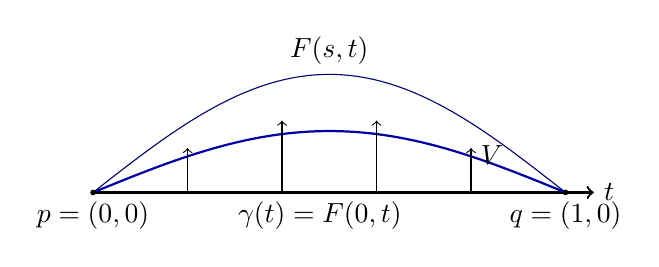
\begin{tikzpicture}[x=6cm,y=1.2cm]
	\draw[thick,->] (0,0)--(1.06,0) node[right] {\(t\)};
	\draw[blue!65!black,thick,domain=0:1,samples=60] plot (\x,{0.65*sin(180*\x)});
	\draw[blue!45!black,domain=0:1,samples=60] plot (\x,{1.25*sin(180*\x)});
	\foreach \x in {0.2,0.4,0.6,0.8}{
		\draw[->] (\x,0)--(\x,{0.8*sin(180*\x)});
	}
	\fill (0,0) circle[x radius=.006,y radius=.03];
	\fill (1,0) circle[x radius=.006,y radius=.03];
	\node[below] at (0,0) {\(p=(0,0)\)};
	\node[below] at (1,0) {\(q=(1,0)\)};
	\node[below] at (.48,0) {\(\gamma(t)=F(0,t)\)};
	\node[above] at (.5,1.25) {\(F(s,t)\)};
	\node[right] at (.8,.4) {\(V\)};
\end{tikzpicture}

	\caption{Euclid 平面上的固定端点变分 \(F(s,t)=(t,s\sin\pi t)\)。箭头表示沿水平基曲线的变分场 \(V=(0,\sin\pi t)\)，两端的场为零。}
	\label{g3:fig:fixed-endpoint-variation}
\end{figure}

沿 \(F\) 的协变导数使用拉回切丛。在任一坐标图中，若 \(Z=Z^k\partial_k|_F\)，则
\[
	(D_tZ)^k=\partial_tZ^k+\Gamma^k_{ij}(F)T^iZ^j,
	\qquad (D_sZ)^k=\partial_sZ^k+\Gamma^k_{ij}(F)S^iZ^j.
\]
因此这些运算不要求 \(F\) 是浸入，也不要求变分曲线互不相交。第二章证明 Gauss 引理时已经用过这种计算；现在还要交换两次协变导数。

\begin{proposition}\label{g3:prop:variation-commutation}
	设 \(F\) 是光滑无边界黎曼流形中的光滑二参数映射，\(T=\partial_tF\)、\(S=\partial_sF\)，\(Z\) 为沿 \(F\) 的光滑向量场。对 Levi-Civita 联络及本卷曲率约定，有
	\begin{equation}\label{g3:eq:variation-commutation}
		D_sT=D_tS,\qquad D_sD_tZ-D_tD_sZ=R(S,T)Z.
	\end{equation}
\end{proposition}
\begin{proof}
	第一式由 \(\partial_s\partial_tF^k=\partial_t\partial_sF^k\) 与 \(\Gamma^k_{ij}=\Gamma^k_{ji}\) 得到，即\eqref{g3:eq:mixed-variation-derivatives}。对第二式展开上面的两次导数，含 \(\partial_s\partial_tZ\)、一阶 \(Z\) 导数以及 \(\partial_sT^i-\partial_tS^i\) 的项相消。余项为
	\[
		\bigl(\partial_i\Gamma^k_{j\ell}-\partial_j\Gamma^k_{i\ell}
		+\Gamma^k_{ir}\Gamma^r_{j\ell}-\Gamma^k_{jr}\Gamma^r_{i\ell}\bigr)
		S^iT^jZ^\ell.
	\]
	由\eqref{g3:eq:curvature-coordinate-components}，这正是 \(R(S,T)Z\) 的第 \(k\) 个分量。
\end{proof}

任意沿 \(\gamma\) 的光滑场都能成为变分场。事实上，第二章的指数映射在零截面附近光滑；\([a,b]\) 紧，故对充分小的共同 \(s\)，可定义
\begin{equation}\label{g3:eq:exponential-field-variation}
	F(s,t)=\exp_{\gamma(t)}(sV(t)).
\end{equation}
由 \((\mathrm d\exp_x)_0=I\)，其变分场为 \(V\)。若 \(V(a)=V(b)=0\)，这个变分固定端点。连续分片光滑场也由同一公式实现为上述分片光滑变分。这里的紧性只涉及所给曲线的参数区间，无须假设整个 \(M\) 完备。

\subsection{第一变分及端点项}
\label{g3:subsec:0601:02}

对分片光滑曲线 \(c:[a,b]\to M\)，定义其\term[quxian nengliang]{能量}[energy]和长度
\begin{equation}\label{g3:eq:curve-energy-length}
	E(c)=\frac12\int_a^b|\dot c|^2\,\mathrm dt,
	\qquad L(c)=\int_a^b|\dot c|\,\mathrm dt.
\end{equation}
\symidx{\(E(c)\)：曲线能量}
长度在保向重参数化下不变，能量还记录行进速度。在固定区间上，Cauchy--Schwarz 不等式给出
\begin{equation}\label{g3:eq:energy-length-inequality}
	L(c)^2\le2(b-a)E(c),
\end{equation}
等号当且仅当速度长度几乎处处为同一个常数。特别地，若连接两端点的常速最短测地线 \(\gamma\) 存在，则
\[
	E(c)\ge \frac{L(c)^2}{2(b-a)}
	\ge\frac{d(\gamma(a),\gamma(b))^2}{2(b-a)}=E(\gamma).
\]
等号要求曲线同时最短且常速。使用能量可以保留测地线参数，又避开长度被积式在零速度处不可微的问题。

\begin{theorem}[第一变分]\label{g3:thm:curve-first-variation}
	设 \(F\) 是光滑无边界黎曼流形中光滑曲线 \(\gamma:[a,b]\to M\) 的光滑变分，\(V=\partial_sF|_{s=0}\)、\(T=\dot\gamma\)。则
	\begin{equation}\label{g3:eq:energy-first-variation}
		\left.\frac{\mathrm d}{\mathrm ds}E(F(s,\cdot))\right|_{s=0}
		=[\langle V,T\rangle]_a^b-\int_a^b\langle V,D_tT\rangle\,\mathrm dt.
	\end{equation}
	若 \(\gamma\) 正则，即 \(|T|>0\)，令 \(U=T/|T|\)，则
	\begin{equation}\label{g3:eq:length-first-variation}
		\left.\frac{\mathrm d}{\mathrm ds}L(F(s,\cdot))\right|_{s=0}
		=[\langle V,U\rangle]_a^b-\int_a^b\langle V,D_tU\rangle\,\mathrm dt.
	\end{equation}
\end{theorem}
\begin{proof}
	度量相容性和\cref{g3:prop:variation-commutation}给出
	\[
		\partial_s\tfrac12|\partial_tF|^2
		=\langle D_sT,T\rangle=\langle D_tS,T\rangle.
	\]
	对紧区间求导积分并分部积分，得到第一式。正则曲线的速度在紧区间上有正下界，所以充分小的变分也正则；此时
	\(\partial_s|T|=\langle D_tS,T/|T|\rangle\)。再次分部积分即得第二式。
\end{proof}

\begin{corollary}\label{g3:cor:energy-critical-geodesic}
	光滑无边界黎曼流形中的光滑曲线，在所有固定端点光滑变分下能量一阶导数为零，当且仅当它是仿射参数测地线。正则曲线在所有这样的变分下长度一阶导数为零，当且仅当它的弧长参数化是测地线。
\end{corollary}
\begin{proof}
	端点项为零。若第一式对所有端点为零的场 \(V\) 消失，取非负紧支函数 \(\chi\) 并用 \(V=\chi D_tT\)，得到 \(\int\chi|D_tT|^2=0\)，所以 \(D_tT=0\)。反向由公式直接成立。长度的情形以 \(D_tU\) 替代 \(D_tT\)，得到 \(D_tU=0\)。因为弧长 \(\ell\) 满足 \(\mathrm d\ell/\mathrm dt=|T|>0\)，这等价于 \(D_\ell U=0\)。
\end{proof}

对分片光滑的基曲线，逐片分部积分还会在每个内节点 \(t_i\) 出现项
\begin{equation}\label{g3:eq:energy-corner-terms}
	\langle V(t_i),T(t_i^-)-T(t_i^+)\rangle.
\end{equation}
允许独立移动节点后，能量驻定要求这些速度跳跃全部为零。长度公式则用单位切向量 \(U\) 的跳跃；它排除角点，但不要求两侧速度大小相等。这与第二章最短曲线可以按弧长参数化为光滑测地线的结论相符。

\subsection{第二变分和曲率项}
\label{g3:subsec:0601:03}

以下在仿射参数测地线处求二次变化。记 \(V'=D_tV\)，并令
\[
	A(t)=(D_sS)(0,t).
\]
\(A\) 是各条 \(s\)-曲线的协变加速度，通常并不为零。一次变分只看 \(V\)；若端点可动，二次变分还会看到端点轨迹的加速度。

\begin{theorem}[能量第二变分]\label{g3:thm:energy-second-variation}
	设 \(\gamma:[a,b]\to M\) 为光滑无边界黎曼流形中的仿射参数测地线，\(F\) 为它的光滑变分，\(V=\partial_sF|_0\)、\(A=D_s\partial_sF|_0\)、\(T=\dot\gamma\)。则
	\begin{equation}\label{g3:eq:energy-second-variation}
		E''(0)=\int_a^b\bigl(|V'|^2-\langle R(V,T)T,V\rangle\bigr)\,\mathrm dt
		+[\langle A,T\rangle]_a^b.
	\end{equation}
	若变分固定端点，最后一项为零。若变分仅沿一个共同有限分割分片光滑，且变分场连续，同式仍按各片积分成立。
\end{theorem}
\begin{proof}
	在变分上对 \(E'(s)=\int\langle D_tS,T\rangle\) 再求导，得
	\[
		E''(0)=\int_a^b\bigl(\langle D_sD_tS,T\rangle+|D_tS|^2\bigr)\big|_{s=0}\,\mathrm dt.
	\]
	交换公式将第一项写成 \(\langle D_tA+R(V,T)V,T\rangle\)。由于 \(D_tT=0\)，对 \(D_tA\) 分部积分只留下端点项。\cref{g3:prop:curvature-symmetries}的斜伴随性质给出
	\[
		\langle R(V,T)V,T\rangle=-\langle R(V,T)T,V\rangle,
	\]
	于是得到所述公式。固定端点时，端点的整条 \(s\)-曲线为常曲线，故 \(A(a)=A(b)=0\)。在分片情形，各接缝处的 \(A\) 连续，基曲线的 \(T\) 也连续，因此内节点的边界项相消。
\end{proof}

当 \(T\) 为单位向量且 \(V\perp T\) 时，曲率项为 \(K(V,T)|V|^2\)。正曲率减小二次变化，负曲率增大二次变化。这是随后共轭点与曲率比较出现相反效应的具体原因。

\ProseParagraphBreak

固定端点时，二次变化只取决于 \(V\)，与实现它的变分的二阶数据无关。极化得到对称双线性形式
\begin{equation}\label{g3:eq:index-form-introduction}
	I_\gamma(V,W)=\int_a^b\bigl(\langle V',W'\rangle
	-\langle R(V,T)T,W\rangle\bigr)\,\mathrm dt.
\end{equation}
曲率对称性保证 \(V\mapsto R(V,T)T\) 自伴，故这个形式确实对称。在固定端点的二参数变分中，混合二阶导数就是 \(I_\gamma(V,W)\)：可把前一公式用于参数平面中每条直线，再由极化恒等式恢复混合项。\secref{g3:sec:0603}将把它作为指标形式系统研究。

\begin{theorem}[长度第二变分]\label{g3:thm:length-second-variation}
	设 \(\gamma:[a,b]\to M\) 为光滑无边界黎曼流形中的单位速测地线，\(F\) 为光滑变分，\(V,A,T\) 如前一定理。令 \(V^\perp=V-\langle V,T\rangle T\)，则
	\begin{align}
		L''(0)&=\int_a^b\bigl(|V'|^2-\langle V',T\rangle^2
		-\langle R(V,T)T,V\rangle\bigr)\,\mathrm dt
		+[\langle A,T\rangle]_a^b\notag\\
		&=I_\gamma(V^\perp,V^\perp)+[\langle A,T\rangle]_a^b.
		\label{g3:eq:length-second-variation}
	\end{align}
\end{theorem}
\begin{proof}
	令 \(q(s,t)=|\partial_tF|^2\)。在 \(s=0\) 处 \(q=1\)，故
	\[
		\partial_s^2\sqrt q=\tfrac12\partial_s^2q-\tfrac14(\partial_sq)^2.
	\]
	第一项积分是能量第二变分，而 \(\partial_sq|_0=2\langle V',T\rangle\)，得到第一行。写 \(V=fT+V^\perp\)，利用 \(D_tT=0\) 可得 \(V'=f'T+(V^\perp)'\)，其中后项仍垂直于 \(T\)。又因 \(R(T,T)=0\) 及 \(R(V^\perp,T)T\perp T\)，曲率项也只看 \(V^\perp\)，于是得到第二行。
\end{proof}

例如在 Euclid 空间中取单位直线段 \(\gamma\)，令 \(f(a)=f(b)=0\)。变分 \(F(s,t)=\gamma(t+sf(t))\) 在小 \(s\) 时只是重参数化，故长度恒定；其变分场是 \(V=fT\)，能量二次变化却为 \(\int_a^b(f')^2\)。长度的切向零方向来自参数自由度，不能将这些方向误认为几何上的共轭方向。

\subsection{固定端点与自由端点的区别}
\label{g3:subsec:0601:04}

现在允许起点在光滑嵌入子流形 \(P\) 内移动、终点在光滑嵌入子流形 \(Q\) 内移动。允许的场满足
\[
	V(a)\in T_{\gamma(a)}P,\qquad V(b)\in T_{\gamma(b)}Q.
\]
这些条件也足以实现变分。为说明这一点，在 \(P,Q\) 内选端点曲线 \(p(s),q(s)\)，其初速度分别是 \(V(a),V(b)\)。先用\eqref{g3:eq:exponential-field-variation}，再在指数映射的输入中加入两端的修正：用沿 \(\gamma\) 的平行运输，把
\[
	\eta_a(s)=\exp_{\gamma(a)}^{-1}p(s)-sV(a),\qquad
	\eta_b(s)=\exp_{\gamma(b)}^{-1}q(s)-sV(b)
\]
分别延到两端的短邻域，并乘以在相应端点为1、另一端附近为0的光滑截断函数。因为 \(\eta_a,\eta_b=O(s^2)\)，修正不改变变分场，却使端点恰落在 \(P,Q\) 上。这个构造也适用于连续分片光滑场。

\begin{proposition}\label{g3:prop:submanifold-endpoint-variation}
	设 \(P,Q\) 为光滑无边界黎曼流形 \((M,g)\) 的光滑嵌入子流形。光滑曲线 \(\gamma:[a,b]\to M\) 的两端分别在 \(P,Q\) 上。它在所有端点留在 \(P,Q\) 的变分下能量驻定，当且仅当它是测地线，且
	\[
		\dot\gamma(a)\perp T_{\gamma(a)}P,\qquad
		\dot\gamma(b)\perp T_{\gamma(b)}Q.
	\]
	在这样的测地线处，第二变分为
	\begin{equation}\label{g3:eq:submanifold-endpoint-hessian}
		E''(0)=I_\gamma(V,V)
		+\langle B^Q(V(b),V(b)),T(b)\rangle
		-\langle B^P(V(a),V(a)),T(a)\rangle,
	\end{equation}
	其中 \(B^P,B^Q\) 为第四章约定的环境法丛值第二基本形式。
\end{proposition}
\begin{proof}
	先取端点为零的场，由\cref{g3:cor:energy-critical-geodesic}得到测地线方程。再独立取两个端点的任意切向量，第一变分的边界项对它们都为零恰好等价于两端的正交性。反向同样由第一变分成立。

	起点轨迹 \(p(s)\) 位于 \(P\)，由\cref{g3:prop:gauss-decomposition}，其环境加速度的法向部分为 \(B^P(V(a),V(a))\)。切向部分与 \(T(a)\) 正交，因此
	\(\langle A(a),T(a)\rangle=\langle B^P(V(a),V(a)),T(a)\rangle\)。终点同理，代入能量第二变分即得公式。
\end{proof}

若只允许起点在 \(P\) 上移动而终点固定，则边界项化为
\[
	-\langle A_{T(a)}^P V(a),V(a)\rangle.
\]
这里形算子的约定是 \(\langle A_\nu X,Y\rangle=\langle B(X,Y),\nu\rangle\)，所以负号来自下端点的减号。\secref{g3:sec:0604}的焦点边界条件将由这一项导出。若“自由端点”指端点可在整个 \(M\) 中任意移动，则能量驻定要求该端速度为零；测地线速度恒定，因而只剩常曲线。非平凡自由边界问题须指定端点所在子流形。

\begin{example}\label{g3:exm:concentric-circles-boundary-hessian}
	在 Euclid 平面中取两条同心圆，半径分别为 \(r\) 和 \(r+\ell\)，其中 \(r,\ell>0\)。径向线段 \(\gamma(t)=(r+t,0)\)、\(0\le t\le\ell\)，垂直连接两圆。旋转变分
	\[
		F(s,t)=(r+t)(\cos s,\sin s)
	\]
	保持每条曲线的长度和能量，因此二次变化为零。其场 \(V=(r+t)e_2\) 却满足 \(I_\gamma(V,V)=\ell\)。按外法向计算，两个形算子分别为 \(-I/r\)、\(-I/(r+\ell)\)，所以边界修正为 \(-(r+\ell)+r=-\ell\)，恰好抵消积分项。这一计算同时核验了两端边界项的次序及形算子的符号。
\end{example}

% !TeX root = ../../Book3.tex
% 纲要标题：### 6.2 Jacobi 场与指数映射
% 纲要位置：几何学计划纲要.md，第 2335 行。
% 正文状态：初稿；尚未正式审核。

% 纲要内容开始
% 
% * Jacobi 方程的推导
% * 初值、Wronskian 配对与解空间
% * 指数映射的微分
% * 共轭点及其重数
% 
% 纲要内容结束

\section{Jacobi 场与指数映射}
\label{g3:sec:0602}

从同一点发出的直线，初始方向稍有改变，分离量便随时间线性增长；球面上从北极发出的经线，却会在南极重新相遇。要描述这种差别，可以让测地线的初始点和初速度随一个参数变化，再对这个参数求导。得到的向量场满足一个由曲率控制的线性方程，这就是 Jacobi\footnote{Carl Gustav Jacob Jacobi（1804--1851），德国数学家，研究椭圆函数、偏微分方程和分析力学。} 方程。它既描述测地线族的一阶分离，也计算指数映射的微分。

\subsection{Jacobi 方程的推导}
\label{g3:subsec:0602:01}

本节设 \((M,g)\) 为 \(n\) 维光滑无边界黎曼流形，\(\gamma:I\to M\) 是仿射参数测地线，\(I\) 为开区间。记 \(T=\dot\gamma\)，对沿 \(\gamma\) 的场简写 \(J'=D_tJ\)、\(J''=D_t^2J\)。特别地，\(T'=0\)。先设 \(F(s,t)\) 是一个光滑测地线变分：\(F(0,t)=\gamma(t)\)，且对每个固定的 \(s\)，曲线 \(t\mapsto F(s,t)\) 都满足测地线方程。令 \(S=\partial_sF\)、\(T_s=\partial_tF\)。由\cref{g3:prop:variation-commutation}，
\[
	0=D_sD_tT_s
	=D_tD_sT_s+R(S,T_s)T_s
	=D_t^2S+R(S,T_s)T_s.
\]
在 \(s=0\) 处取值，变分场 \(J(t)=S(0,t)\) 因而满足
\begin{equation}\label{g3:eq:jacobi-equation}
	J''+R(J,T)T=0.
\end{equation}
正号由本卷 \(R(X,Y)=\nabla_X\nabla_Y-\nabla_Y\nabla_X-\nabla_{[X,Y]}\) 的约定决定。例如正曲率球面上的法向分离量将满足振子方程，而不是指数增长方程。

\begin{definition}[Jacobi 场]\label{g3:def:jacobi-field}
	设 \(\gamma:I\to M\) 是光滑黎曼流形 \((M,g)\) 中的仿射参数测地线，\(T=\dot\gamma\)，\(D_t\) 为沿线协变导数，\(R\) 为 Levi-Civita 曲率。满足 Jacobi 方程 \(D_t^2J+R(J,T)T=0\)（式\eqref{g3:eq:jacobi-equation}）的光滑沿曲线向量场 \(J\)，称为沿 \(\gamma\) 的\term[Jacobi chang]{Jacobi 场}[Jacobi field]。全体这样的场构成实向量空间，记为 \(\mathcal J(\gamma)\)。
\end{definition}
\symidx{\(\mathcal J(\gamma)\)：沿测地线的 Jacobi 场空间}

刚才已经证明，测地线变分的变分场必为 Jacobi 场。反向命题也成立：给定一个 Jacobi 场，可以改变测地线的初始数据，使它成为所得到测地线族的变分场。这个构造依赖线性方程初值的唯一性，将在下一小节完成。

\ProseParagraphBreak

方程中的线性算子 \(\mathcal R_t:V\mapsto R(V,T)T\) 有两个关键性质。由曲率反对称性，它消去 \(T\)；由\cref{g3:prop:curvature-symmetries}的两对交换对称性，
\begin{equation}\label{g3:eq:jacobi-curvature-self-adjoint}
	\langle\mathcal R_tU,V\rangle
	=\mathrm{Rm}(U,T,V,T)
	=\mathrm{Rm}(V,T,U,T)
	=\langle U,\mathcal R_tV\rangle.
\end{equation}
因此 \(\mathcal R_t\) 自伴，而且保持 \(T^\perp\)。这使切向变化与法向变化能够分开处理，也将给出两个解之间的一个守恒配对。

\subsection{初值、Wronskian 配对与解空间}
\label{g3:subsec:0602:02}

二阶方程需要同时指定位置与一阶导数。这里的“位置”是沿测地线的向量 \(J(t_0)\)，一阶导数则是 \(J'(t_0)\)，二者都属于同一个切空间。

\begin{theorem}\label{g3:thm:jacobi-initial-data}
	下文 \(\mathcal J(\gamma)\) 表示沿 \(\gamma\) 的 Jacobi 场空间，撇号表示沿线 Levi-Civita 协变导数。
	设 \(\gamma:I\to M\) 为 \(n\) 维光滑黎曼流形中的仿射参数测地线，\(t_0\in I\)。对任意 \(v,w\in T_{\gamma(t_0)}M\)，存在唯一 \(J\in\mathcal J(\gamma)\) 满足
	\[
		J(t_0)=v,\qquad J'(t_0)=w.
	\]
	该解存在于整个 \(I\)，并线性依赖 \((v,w)\)。特别地，初值映射
	\begin{equation}\label{g3:eq:jacobi-initial-isomorphism}
		\mathcal J(\gamma)\longrightarrow
		T_{\gamma(t_0)}M\oplus T_{\gamma(t_0)}M,
		\qquad J\longmapsto(J(t_0),J'(t_0))
	\end{equation}
	是线性同构，故 \(\dim\mathcal J(\gamma)=2n\)。在光滑参数族中，解在共同的紧时间区间上光滑依赖测地线及初始数据。
\end{theorem}
\begin{proof}
	把 \(T_{\gamma(t_0)}M\) 的一个正交单位基沿 \(\gamma\) 平行移动，得到平行正交标架 \(e_1(t),\ldots,e_n(t)\)。所用存在性和参数依赖是第一卷第15章第2节“沿路径的平行移动”中的平行移动定理；在开区间上，先在包含 \(t_0\) 的紧子区间上构造，再由唯一性粘合。度量相容性保证标架始终正交。若 \(J=\sum_i j^ie_i\)，则 \(J'=\sum_i(j^i)'e_i\)，方程化为
	\begin{equation}\label{g3:eq:jacobi-matrix-equation}
		j''+\mathcal R(t)j=0,
		\qquad \mathcal R_{ij}(t)=\langle R(e_j,T)T,e_i\rangle.
	\end{equation}
	矩阵 \(\mathcal R(t)\) 光滑且对称。令 \(z=(j,j')^{\mathsf T}\)，便得到一阶线性系统
	\[
		z'=\begin{pmatrix}0&I_n\\-\mathcal R(t)&0\end{pmatrix}z.
	\]
	第一卷同节的“线性方程的全区间解”引理适用于这个 \(2n\) 阶系统，给出每个紧子区间上的唯一解、线性初值依赖及光滑参数依赖。用包含 \(t_0\) 的紧子区间穷尽 \(I\)，相邻解由唯一性一致，遂得到整个 \(I\) 上的解。初值映射的双射性和维数结论随即成立。对于参数族，在参数点附近先平滑选择初始正交标架，再作平行移动；上述矩阵系统的系数便光滑依赖参数，同一引理给出最后的断言。
\end{proof}

\begin{proposition}\label{g3:prop:jacobi-geodesic-variation}
	设 \((M,g)\) 为光滑无边界黎曼流形，\(J\) 为沿仿射参数测地线 \(\gamma:I\to M\) 的 Jacobi 场，\([a,b]\subset I\) 为紧区间。则存在 \(\varepsilon>0\) 和光滑测地线变分 \(F:(-\varepsilon,\varepsilon)\times[a,b]\to M\)，其中心曲线为 \(\gamma\)，变分场为 \(J\)。
\end{proposition}
\begin{proof}
	选 \(t_0\in[a,b]\)，记 \(p=\gamma(t_0)\)、\(v=J(t_0)\)、\(w=J'(t_0)\)。取 \(p(s)=\exp_p(sv)\)，并令 \(P_s:T_pM\to T_{p(s)}M\) 为沿这条短曲线从 \(0\) 到 \(s\) 的平行移动。定义初速度
	\[
		u(s)=P_s\bigl(T(t_0)+sw\bigr).
	\]
	于是 \(p'(0)=v\)，且沿 \(p(s)\) 的协变导数满足 \(D_su(0)=w\)。由\cref{g3:thm:geodesic-ivp}，取初始点 \(p(s)\)、初速度 \(u(s)\)，在时刻 \(t_0\) 出发，得到测地线族 \(F(s,t)\)。测地线流的定义域开，中心解的参数区间 \([a,b]\) 紧，故缩小 \(\varepsilon\) 后，所有这些曲线都在整个 \([a,b]\) 上存在并联合光滑。

	变分场 \(\widetilde J\) 满足 Jacobi 方程，且 \(\widetilde J(t_0)=v\)。交换一次协变导数还给出
	\[
		\widetilde J'(t_0)
		=D_t\partial_sF(0,t_0)
		=D_s\partial_tF(0,t_0)=D_su(0)=w.
	\]
	由\cref{g3:thm:jacobi-initial-data}，\(\widetilde J=J\)。
\end{proof}

给定 Jacobi 场以后，这个实现只需改变初始点和初速度。若要求变分中的测地线全都具有单位速度，还要额外满足 \(\langle J',T\rangle=0\)；下文的切向分解会说明这个量为何恒定。

\begin{proposition}\label{g3:prop:jacobi-wronskian}
	下文 \(\mathcal J(\gamma)\) 表示沿 \(\gamma\) 的 Jacobi 场空间，撇号表示沿线 Levi-Civita 协变导数。
	设 \((M^n,g)\) 为光滑黎曼流形，\(\gamma:I\to M\) 为仿射参数测地线，\(t_0\in I\)，\(J,K\) 是沿 \(\gamma\) 的 Jacobi 场。它们的\term[Wronskian peidui]{Wronskian 配对}[Wronskian pairing]\footnote{Józef Maria Hoëné-Wroński（1776--1853），波兰裔法国数学家、哲学家，其函数展开研究涉及后来称为 Wronskian 的行列式。}定义为
	\begin{equation}\label{g3:eq:jacobi-wronskian}
		W(J,K)=\langle J',K\rangle-\langle J,K'\rangle.
	\end{equation}
	右端与参数 \(t\) 无关，并在 \(\mathcal J(\gamma)\) 上给出非退化的交替双线性配对。对任一 \(t_0\)，子空间
	\[
		\mathcal J_{t_0}(\gamma)=\{J\in\mathcal J(\gamma):J(t_0)=0\}
	\]
	维数为 \(n\)，且其中任意两个场的 \(W\) 配对均为零。
\end{proposition}
\symidx{\(W(J,K)\)：Jacobi 场的 Wronskian 配对}
\begin{proof}
	由 Jacobi 方程及式\eqref{g3:eq:jacobi-curvature-self-adjoint}，
	\[
		\frac{\mathrm d}{\mathrm dt}
		\bigl(\langle J',K\rangle-\langle J,K'\rangle\bigr)
		=\langle-\mathcal R_tJ,K\rangle+\langle J,\mathcal R_tK\rangle=0.
	\]
	交替性和双线性由定义直接得到。在初值同构\eqref{g3:eq:jacobi-initial-isomorphism}下，若 \(J\) 对应 \((v,w)\)、\(K\) 对应 \((u,z)\)，则
	\[
		W(J,K)=\langle w,u\rangle-\langle v,z\rangle.
	\]
	如果此值对所有 \(K\) 都为零，取 \((u,z)=(w,-v)\)，可得 \(|w|^2+|v|^2=0\)，故 \(J=0\)。最后，\(J(t_0)=0\) 的场由任意 \(J'(t_0)\) 唯一决定，维数为 \(n\)；当 \(J,K\) 都在 \(t_0\) 消失时，在该时刻计算 \(W\) 即得零。
\end{proof}

\begin{proposition}\label{g3:prop:jacobi-tangential-normal}
	设 \((M,g)\) 为光滑黎曼流形，\(\gamma:I\to M\) 为单位速测地线，\(T=\dot\gamma\)，\(t_0\in I\)，撇号表示沿线协变导数。每个 Jacobi 场唯一分解为
	\begin{equation}\label{g3:eq:jacobi-tangential-normal}
		J(t)=\bigl(a+b(t-t_0)\bigr)T(t)+J^\perp(t),
		\qquad J^\perp(t)\perp T(t),
	\end{equation}
	其中 \(J^\perp\) 仍为 Jacobi 场，\(a=\langle J(t_0),T(t_0)\rangle\)、\(b=\langle J'(t_0),T(t_0)\rangle\)。特别地，\(J\) 处处垂直于 \(T\)，当且仅当这两个初始内积均为零；若 \(J\) 在两个不同时刻消失，则它处处垂直于 \(T\)。
\end{proposition}
\begin{proof}
	令 \(f=\langle J,T\rangle\)。因为 \(T'=0\)、\(\mathcal R_tT=0\) 且 \(\mathcal R_t\) 自伴，
	\[
		f''=\langle J'',T\rangle=-\langle\mathcal R_tJ,T\rangle=0.
	\]
	故 \(f(t)=a+b(t-t_0)\)。场 \(fT\) 满足 Jacobi 方程，因而 \(J-fT\) 也满足，并与 \(T\) 正交。其余结论来自一次函数的初值和零点性质。
\end{proof}

\begin{example}\label{g3:exm:constant-curvature-jacobi}
	设光滑黎曼流形 \((M,g)\) 具有常截面曲率 \(k\in\mathbb R\)，\(\gamma:I\to M\) 为单位速测地线，\(0\in I\)，\(T=\dot\gamma\)，撇号表示沿线协变导数。记从 \(0\) 到 \(t\) 的平行移动为 \(P_t\)，定义
	\begin{equation}\label{g3:eq:model-jacobi-functions}
		s_k(t)=
		\begin{cases}
			\sin(\sqrt{k}\,t)/\sqrt{k},&k>0,\\
			t,&k=0,\\
			\sinh(\sqrt{-k}\,t)/\sqrt{-k},&k<0,
		\end{cases}
		\qquad c_k(t)=s_k'(t).
	\end{equation}
	若 \(J(0)=aT(0)+u\)、\(J'(0)=bT(0)+v\)，其中 \(u,v\perp T(0)\)，则
	\begin{equation}\label{g3:eq:constant-curvature-jacobi-solution}
		J(t)=(a+bt)T(t)+P_t\bigl(c_k(t)u+s_k(t)v\bigr).
	\end{equation}
	事实上，常曲率公式\eqref{g3:eq:constant-sectional-algebraic}给出
	\[
		R(V,T)T=k\bigl(V-\langle V,T\rangle T\bigr).
	\]
	法向部分在平行标架中满足 \(j''+kj=0\)，而 \(c_k,s_k\) 的初值分别为 \((1,0)\)、\((0,1)\)。验证方程与初值后，\cref{g3:thm:jacobi-initial-data}即证明所列公式。由同一起点出发时 \(u=a=0\)，法向分离量由 \(s_k(t)\) 控制：正曲率下可以再次消失，零曲率下线性增长，负曲率下则含双曲正弦因子。
\end{example}
\symidx{\(s_k,c_k\)：常曲率 Jacobi 方程的标准解}

\subsection{指数映射的微分}
\label{g3:subsec:0602:03}

固定 \(p\in M\)。第二章已经定义指数映射 \(\exp_p:\mathcal E_p\to M\)，其中 \(\mathcal E_p\subset T_pM\) 为包含零的开星形集。要对 \(\exp_p\) 在向量 \(v\) 处沿 \(w\) 求导，只须改变初速度为 \(v+sw\)。这一变化恰好属于刚才研究的测地线变分。

\begin{proposition}\label{g3:prop:exponential-differential-jacobi}
	设 \((M,g)\) 为光滑无边界黎曼流形，\(\mathcal E_p\) 为指数映射 \(\exp_p\) 的定义域，撇号表示沿线协变导数。
	设 \(p\in M\)、\(v\in\mathcal E_p\)、\(w\in T_pM\)，令 \(\gamma_v(t)=\exp_p(tv)\)，\(0\le t\le1\)。沿此测地线取初值为
	\[
		J_w(0)=0,\qquad J_w'(0)=w
	\]
	的 Jacobi 场，则
	\begin{equation}\label{g3:eq:exponential-differential-jacobi}
		J_w(t)=(\mathrm d\exp_p)_{tv}(tw),
		\qquad (\mathrm d\exp_p)_v(w)=J_w(1).
	\end{equation}
	这里通过向量空间的自然平移，把 \(T_{tv}(T_pM)\) 识别为 \(T_pM\)。更一般地，若 \(\gamma(t)=\exp_p(tu)\) 定义在含 \(0\) 的区间上，\(J_w(0)=0\)、\(J_w'(0)=w\)，则对 \(t\ne0\) 有
	\begin{equation}\label{g3:eq:exponential-differential-time-scaling}
		(\mathrm d\exp_p)_{tu}(w)=\frac1tJ_w(t).
	\end{equation}
\end{proposition}
\begin{proof}
	由 \(\mathcal E_p\) 的开性，充分小的 \(s\) 满足 \(v+sw\in\mathcal E_p\)，星形性又保证
	\[
		F(s,t)=\exp_p\bigl(t(v+sw)\bigr),\qquad 0\le t\le1,
	\]
	有定义。对固定 \(s\)，这是初始速度为 \(v+sw\) 的测地线。其变分场 \(J\) 为 Jacobi 场，且因为 \(F(s,0)=p\)，有 \(J(0)=0\)。在起点交换导数，得到
	\[
		J'(0)=D_s\partial_tF(s,0)\big|_{s=0}
		=\left.\frac{\mathrm d}{\mathrm ds}(v+sw)\right|_{s=0}=w.
	\]
	唯一性说明 \(J=J_w\)，而链式法则给出 \(J(t)=(\mathrm d\exp_p)_{tv}(tw)\)。在 \(t=1\) 处即得第二式。对一般固定的 \(t\)，在包含 \(0,t\) 的紧区间上作同样的变分，或用测地线的仿射重参数化，得到 \(J_w(t)=(\mathrm d\exp_p)_{tu}(tw)\)；再用微分的线性性即得式\eqref{g3:eq:exponential-differential-time-scaling}。
\end{proof}

因子 \(1/t\) 记录了两种参数的区别：\(J_w'(0)=w\) 改变的是初速度，而在 \(tu\) 处取微分改变的是时间 \(t\) 后的指数映射自变量。沿径向取 \(w=u\) 时，唯一的初值解是 \(J_u(t)=t\dot\gamma(t)\)，因而
\[
	(\mathrm d\exp_p)_{tu}(u)=\dot\gamma(t).
\]
所以非零径向方向始终被映为非零向量。指数映射若发生奇异，原因必来自与径向正交的方向。

\begin{example}\label{g3:exm:model-exponential-differential}
	取 \(k\in\mathbb R\)。记 \(s_k\) 为 \(s_k''+ks_k=0\)、\(s_k(0)=0\)、\(s_k'(0)=1\) 的解，\(c_k=s_k'\)、\(\operatorname{ct}_k=c_k/s_k\)，\(b_k=\pi/\sqrt k\) 当 \(k>0\)，否则 \(b_k=\infty\)。
	在常曲率 \(k\) 的流形中，令 \(u\in T_pM\) 为单位向量，\(r>0\)，且测地线 \(\gamma(t)=\exp_p(tu)\) 定义到 \(r\)。对 \(w\perp u\)、\(a\in\mathbb R\)，\cref{g3:exm:constant-curvature-jacobi}及式\eqref{g3:eq:exponential-differential-time-scaling}给出
	\begin{equation}\label{g3:eq:model-exponential-differential}
		(\mathrm d\exp_p)_{ru}(au+w)
		=P_r\left(au+\frac{s_k(r)}r w\right).
	\end{equation}
	径向伸缩率为 \(1\)，横向伸缩率为 \(s_k(r)/r\)。当 \(r\to0\) 时，这个比值趋于 \(1\)，与 \((\mathrm d\exp_p)_0=I\) 相符。半径为 \(a_0\) 的圆球面上，它等于 \(a_0\sin(r/a_0)/r\)，在首次到达对径点时为零；平坦情形恒为 \(1\)。
\end{example}

\subsection{共轭点及其重数}
\label{g3:subsec:0602:04}

若一个非零 Jacobi 场在测地线段的两端都消失，它描述了端点在一阶上保持不动的测地线变化。这是后面指标型出现零方向的来源。定义必须保留所选的测地线段：同一对点可以由不同测地线连接，它们的线性化行为未必相同。

\begin{definition}[共轭点与重数]\label{g3:def:conjugate-point}
	设 \((M,g)\) 为光滑黎曼流形，\(\gamma:I\to M\) 是仿射参数测地线，\(\mathcal J(\gamma)\) 表示沿线 Jacobi 场空间，\(a,b\in I\)、\(a\ne b\)。若存在非零 Jacobi 场 \(J\) 满足 \(J(a)=J(b)=0\)，就称 \(\gamma(a)\) 与 \(\gamma(b)\) 沿该测地线段\term[gonge dian]{共轭}[conjugate]，并把
	\begin{equation}\label{g3:eq:conjugate-multiplicity}
		m_\gamma(a,b)
		=\dim\{J\in\mathcal J(\gamma):J(a)=J(b)=0\}
	\end{equation}
	称为该\term[gonge dian chongshu]{共轭点的重数}[multiplicity of a conjugate point]。固定 \(a\) 后，满足此条件的 \(b\) 称为相对 \(a\) 的共轭时刻。
\end{definition}
\symidx{\(m_\gamma(a,b)\)：沿指定测地线段的共轭重数}

非恒定测地线可以作常数倍重参数化成为单位速度曲线，而 Jacobi 方程在这种变换下保持形式。由\cref{g3:prop:jacobi-tangential-normal}，两端消失的 Jacobi 场必为法向场；它由起点的法向导数决定，故
\[
	0\le m_\gamma(a,b)\le n-1.
\]
恒定测地线上曲率项为零，平行标架中的解是一次函数，在两个不同时刻消失就只能为零。因此恒定测地线没有共轭时刻，一维黎曼流形中也没有共轭时刻。

\begin{proposition}\label{g3:prop:conjugate-exp-singularity}
	设 \((M,g)\) 为光滑无边界黎曼流形，\(\gamma:I\to M\) 为仿射参数测地线，\(m_\gamma\) 表示式\eqref{g3:eq:conjugate-multiplicity}的共轭重数，\(0\in I\)，\(p=\gamma(0)\)、\(u=\dot\gamma(0)\)。对 \(t_0\in I\setminus\{0\}\)，点 \(\gamma(t_0)\) 与 \(p\) 沿此段共轭，当且仅当 \((\mathrm d\exp_p)_{t_0u}\) 奇异，而且
	\begin{equation}\label{g3:eq:conjugate-exp-nullity}
		m_\gamma(0,t_0)=\dim\ker(\mathrm d\exp_p)_{t_0u}.
	\end{equation}
\end{proposition}
\begin{proof}
	满足 \(J(0)=0\) 的 Jacobi 场与初始导数 \(w=J'(0)\) 一一对应。由\cref{g3:prop:exponential-differential-jacobi}，
	\[
		J_w(t_0)=(\mathrm d\exp_p)_{t_0u}(t_0w).
	\]
	乘以非零数 \(t_0\) 是 \(T_pM\) 的同构，所以两边的核同维。定义立即给出结论。
\end{proof}

在非共轭时刻，逆函数定理保证所选初速度附近的测地线可以由终点光滑参数化。共轭时刻则存在非零的初速度变化，使终点的一阶变化为零。这一结论是线性化的陈述；它本身没有断言存在一族端点严格固定的不同测地线。

\begin{corollary}\label{g3:cor:jacobi-boundary-value}
	设 \((M,g)\) 为光滑无边界黎曼流形，\(a<b\)，\(\gamma:[a,b]\to M\) 为延拓到端点邻域的测地线，且两端沿此段不共轭。对任意 \(v\in T_{\gamma(a)}M\)、\(w\in T_{\gamma(b)}M\)，存在唯一 Jacobi 场满足 \(J(a)=v\)、\(J(b)=w\)。
\end{corollary}
\begin{proof}
	先取初值为 \((v,0)\) 的 Jacobi 场 \(J_0\)。映射
	\[
		T_{\gamma(a)}M\longrightarrow T_{\gamma(b)}M,
		\qquad z\longmapsto J_z(b),\quad
		J_z(a)=0,\quad J_z'(a)=z,
	\]
	的核由共轭定义为零；源和靶都是 \(n\) 维，所以它是同构。唯一选择 \(z\) 使 \(J_z(b)=w-J_0(b)\)，即可取 \(J=J_0+J_z\)。
\end{proof}

下一结论保证，在一个有限测地线段上，按重数逐个计数共轭时刻是有限过程。证明只使用光滑系数和初值唯一性，并不要求度量解析。

\begin{proposition}\label{g3:prop:conjugate-times-isolated}
	设 \(\gamma:I\to M\) 是光滑黎曼流形中的测地线，\(0\in I\)。相对 \(0\) 的每个共轭时刻在 \(I\) 中孤立；\(0\) 的某个穿孔邻域没有共轭时刻。因此每个紧子区间 \([a,b]\subset I\) 只含有限个相对 \(0\) 的共轭时刻，各自的重数有限。
\end{proposition}
\begin{proof}
	在沿 \(\gamma\) 的平行正交标架中，取矩阵方程
	\[
		Y''+\mathcal R(t)Y=0,\qquad Y(0)=0,\qquad Y'(0)=I_n.
	\]
	其第 \(i\) 列是初始导数为第 \(i\) 个基向量、初始值为零的 Jacobi 场。于是 \(t\ne0\) 为共轭时刻当且仅当 \(Y(t)\) 奇异，重数为 \(\dim\ker Y(t)\)。由 \(Y(t)=tI_n+O(t^2)\)，矩阵 \(Y(t)/t\) 趋于 \(I_n\)，所以 \(0\) 附近没有非零的共轭时刻。

	固定一个共轭时刻 \(t_0\ne0\)，写
	\[
		K=\ker Y(t_0),\qquad L=\operatorname{im}Y(t_0),
		\qquad C=L^\perp,\qquad m=\dim K=\dim C.
	\]
	Wronskian 配对在初始时刻为零，因而对所有 \(t\) 有
	\begin{equation}\label{g3:eq:jacobi-matrix-wronskian}
		Y(t)^{\mathsf T}Y'(t)=Y'(t)^{\mathsf T}Y(t).
	\end{equation}
	若 \(u\in K\)，则对任意 \(v\in\mathbb R^n\)，此式给出
	\[
		\langle Y'(t_0)u,Y(t_0)v\rangle
		=\langle Y(t_0)u,Y'(t_0)v\rangle=0.
	\]
	故 \(Y'(t_0)K\subset C\)。若还满足 \(Y'(t_0)u=0\)，则 Jacobi 场 \(Y(t)u\) 在 \(t_0\) 的值和导数都为零，由初值唯一性它恒为零，再在 \(0\) 处求导便得 \(u=0\)。维数相同于是说明
	\begin{equation}\label{g3:eq:jacobi-kernel-cokernel-isomorphism}
		B=Y'(t_0)|_K:K\longrightarrow C
	\end{equation}
	是同构。这是控制奇异时刻的关键：在消失的方向上，一阶导数恰好补满值域缺少的方向。

	现在按定义域 \(K^\perp\oplus K\) 和值域 \(L\oplus C\) 分块，令 \(\tau=t-t_0\)，写成
	\[
		Y(t)=\begin{pmatrix}A(t)&E(t)\\ F(t)&G(t)\end{pmatrix}.
	\]
	在 \(t_0\) 处，\(A(t_0):K^\perp\to L\) 可逆，其他三块均为零。Taylor 展开及式\eqref{g3:eq:jacobi-kernel-cokernel-isomorphism}给出
	\[
		E(t)=O(\tau),\qquad F(t)=O(\tau),\qquad
		G(t)=\tau B+O(\tau^2).
	\]
	当 \(t\) 接近 \(t_0\) 时，\(A(t)\) 仍可逆。以可逆块矩阵作消元，\(Y(t)\) 可逆等价于下面的补块可逆：
	\begin{equation}\label{g3:eq:jacobi-singular-block}
		G(t)-F(t)A(t)^{-1}E(t)
		=\tau B+O(\tau^2)=\tau\bigl(B+O(\tau)\bigr).
	\end{equation}
	因为 \(B\) 可逆，对充分小的非零 \(\tau\)，此块可逆，故 \(Y(t)\) 可逆。当 \(K^\perp\) 为零空间时，直接使用 \(Y(t)=\tau B+O(\tau^2)\) 即可。于是 \(t_0\) 是孤立共轭时刻。

	最后，假如某个紧子区间含无限多个不同的共轭时刻，就有一个收敛子列，其极限仍在 \(I\) 中。极限不能为 \(0\)，因为 \(0\) 附近已经排除了共轭时刻；若极限非零，则由 \(\det Y\) 的连续性它仍为共轭时刻，与刚证的孤立性矛盾。因此数目有限，重数则由有限维核给出。
\end{proof}

\begin{example}\label{g3:exm:model-conjugate-points}
	取 \(k\in\mathbb R\)。记 \(s_k\) 为 \(s_k''+ks_k=0\)、\(s_k(0)=0\)、\(s_k'(0)=1\) 的解，\(c_k=s_k'\)、\(\operatorname{ct}_k=c_k/s_k\)，\(b_k=\pi/\sqrt k\) 当 \(k>0\)，否则 \(b_k=\infty\)。
	在半径 \(a_0\) 的圆球面 \(S^n(a_0)\)、\(n\ge2\) 上，沿单位速度测地线且以 \(0\) 为初时刻，满足 \(J(0)=0\) 且处处法向的 Jacobi 场恰为
	\[
		J(t)=a_0\sin(t/a_0)P_tv,\qquad v\perp T(0).
	\]
	因此正共轭时刻是 \(\pi a_0,2\pi a_0,3\pi a_0,\ldots\)，每个重数为 \(n-1\)。第一个对应对径点，第二个已经回到初始点；共轭关系记录的是所走的测地线段。

	在常曲率 \(k\le0\) 的模型中，\(s_k(t)\) 对 \(t\ne0\) 不为零，因而没有共轭时刻。圆周 \(S^1(a_0)\) 也没有共轭时刻，因为它没有非零法向方向；但指数映射具有周期 \(2\pi a_0\)，并非单射。这个例子说明，指数映射处处微分可逆，与它在整个切空间上单射，是两个不同的问题。
\end{example}
% 纲要条目排为编号小节标题，并进入目录与书签；说明段仍保留于纲要注释中。

% !TeX root = ../../Book3.tex
% 纲要标题：### 6.3 指标形式和最短性
% 纲要位置：几何学计划纲要.md，第 2342 行。
% 正文状态：初稿；尚未正式审核。

% 纲要内容开始
% 
% * 分段光滑场与指标形式
% * Jacobi 场的极小性质
% * 共轭点前后的符号变化
% * 割点与共轭点的关系
% 
% 纲要内容结束

\section{指标形式和最短性}
\label{g3:sec:0603}

第二变分把能量的变化写成沿测地线的一个二次式。这个式子一方面含有变分场的导数，衡量弯离原曲线的代价；另一方面含有曲率，可能抵消这种代价。Jacobi 场恰好满足相应的驻定方程。本节把这三个对象放在一起，判断二次变分何时为正、何时出现零方向，以及何时能构造真正缩短曲线的变分。

\subsection{分段光滑场与指标形式}
\label{g3:subsec:0603:01}

设 \((M,g)\) 为无边界光滑黎曼流形，\(\gamma:[0,\ell]\to M\) 是单位速测地线，\(\ell>0\)，记 \(T=\dot\gamma\)、\(V'=\mathrm D_tV=\nabla_TV\)。我们允许变分场在有限个参数值处改变导数，这样便能截断 Jacobi 场或逐段拼接它们。场本身仍须连续，否则它不能描述连续曲线的一阶变化。

\begin{definition}\label{g3:def:index-form}
	设 \((M,g)\) 为光滑无边界黎曼流形，\(\ell>0\)。沿单位速测地线 \(\gamma:[0,\ell]\to M\)，记 \(\mathcal V(\gamma)\) 为连续且在某个有限分割的各闭子区间上光滑的向量场空间，记
	\[
		\mathcal V_0(\gamma)=
		\{V\in\mathcal V(\gamma):V(0)=V(\ell)=0\}.
	\]
	记 \(T=\dot\gamma\)、\(R\) 为 Levi-Civita 曲率，撇号表示沿线协变导数。对 \(V,W\in\mathcal V(\gamma)\)，双线性形式
	\begin{equation}\label{g3:eq:index-form}
		I_\gamma(V,W)=
		\int_0^\ell
		\bigl(\langle V',W'\rangle
		-\langle R(V,T)T,W\rangle\bigr)\,\mathrm dt
	\end{equation}
	称为 \(\gamma\) 的\term[zhibiaoxingshi]{指标形式}[index form]。省略下标时写作 \(I\)，并记 \(I(V)=I(V,V)\)。\symidx{\(I_\gamma\)：沿测地线 \(\gamma\) 的指标形式}
\end{definition}

积分按共同细分逐段计算，改变分割不改变积分。由曲率的对称性\cref{g3:prop:curvature-symmetries}，算子 \(V\mapsto R(V,T)T\) 自伴，故 \(I\) 对称。对固定端点变分，\cref{g3:thm:energy-second-variation}给出
\[
	\left.\frac{\mathrm d^2}{\mathrm ds^2}\right|_{s=0}
	E(\gamma_s)=I(V),
	\qquad
	E(c)=\frac12\int_0^\ell|\dot c|^2\,\mathrm dt.
\]
对于分段光滑变分，同样的公式可在各段应用；在内部节点，基准曲线 \(\gamma\) 的速度两侧相同，节点加速度项互相抵消。任意 \(V\in\mathcal V_0(\gamma)\) 都能实现为这种变分的变分场：取
\[
	\gamma_s(t)=\exp_{\gamma(t)}(sV(t)).
\]
紧参数区间及指数映射在零截面附近的定义域保证，对统一的小 \(|s|\) 此式有定义；节点处两侧值相同，端点固定。

\begin{proposition}\label{g3:prop:index-form-integration-by-parts}
	记 \(I=I_\gamma\) 为式\eqref{g3:eq:index-form}的指标形式，\(T=\dot\gamma\)，撇号表示沿线协变导数，\(\mathcal V(\gamma)\) 为连续分段光滑沿线场，\(\mathcal V_0(\gamma)\) 为其中两端为零的场空间。
	设 \(\gamma:[0,\ell]\to M\) 是无边界光滑黎曼流形中的单位速测地线，\(V,W\in\mathcal V(\gamma)\)，并在共同分割
	\(0=t_0<t_1<\cdots<t_m=\ell\) 上光滑。记
	\([V']_j=V'(t_j+)-V'(t_j-)\)。则
	\begin{align}
		I(V,W)
		={}&\langle V'(\ell-),W(\ell)\rangle
			-\langle V'(0+),W(0)\rangle \notag\\
		&-\sum_{j=1}^{m-1}\langle[V']_j,W(t_j)\rangle
			-\sum_{j=1}^m\int_{t_{j-1}}^{t_j}
			\langle V''+R(V,T)T,W\rangle\,\mathrm dt .
		\label{g3:eq:index-form-parts}
	\end{align}
\end{proposition}
\begin{proof}
	度量相容性给出
	\[
		\frac{\mathrm d}{\mathrm dt}\langle V',W\rangle
		=\langle V'',W\rangle+\langle V',W'\rangle.
	\]
	在各段积分后相加。内节点的贡献为
	\(\langle V'(t_j-),W(t_j)\rangle-
	\langle V'(t_j+),W(t_j)\rangle\)，正是负的跳跃项；两端只各留一项，得到所述公式。
\end{proof}

\begin{proposition}\label{g3:prop:index-form-kernel}
	记 \(I=I_\gamma\) 为式\eqref{g3:eq:index-form}的指标形式，\(T=\dot\gamma\)，撇号表示沿线协变导数，\(\mathcal V(\gamma)\) 为连续分段光滑沿线场，\(\mathcal V_0(\gamma)\) 为其中两端为零的场空间。
	设 \(\gamma:[0,\ell]\to M\) 是无边界光滑黎曼流形中的单位速测地线。指标形式在 \(\mathcal V_0(\gamma)\) 上的核
	\[
		\{V\in\mathcal V_0(\gamma):I(V,W)=0
		\text{ 对所有 }W\in\mathcal V_0(\gamma)\}
	\]
	恰为满足 \(J(0)=J(\ell)=0\) 的光滑 Jacobi 场空间。
\end{proposition}
\begin{proof}
	若 \(J\) 是这样的 Jacobi 场，式\eqref{g3:eq:index-form-parts}中的积分、跳跃及端点项全部为零，故 \(J\) 属于核。反过来，在每段内部取任意紧支撑光滑测试场，核条件迫使
	\(V''+R(V,T)T=0\)。这里可在平行标架中逐分量使用连续函数的基本引理：若某分量在一点非零，则在其同号小邻域取非负测试函数即可得到非零积分。于是 \(V\) 在每段都是 Jacobi 场。再取仅在某一节点附近非零、且节点值任意的连续光滑场，式\eqref{g3:eq:index-form-parts}给出 \([V']_j=0\)。相邻两段具有相同的位置及一阶导数，Jacobi 初值唯一性使它们接成同一个光滑解。
\end{proof}

\(I(V)=0\) 与 \(V\) 属于上述核一般不能等同；若 \(I\) 半正定，则二者等价。切向与法向部分也可分开：若 \(V=fT+V^\perp\)、\(W=hT+W^\perp\)，则
\begin{equation}\label{g3:eq:index-tangential-normal-split}
	I(V,W)=\int_0^\ell f'h'\,\mathrm dt+I(V^\perp,W^\perp).
\end{equation}
这是因为 \(T'=0\)、\(R(T,T)=0\)，而法向场及其沿线导数都垂直于 \(T\)。固定端点长度第二变分为 \(I(V^\perp)\)，见\cref{g3:thm:length-second-variation}；切向变分的一部分只改变参数。

\begin{lemma}\label{g3:lem:short-interval-index-positive}
	记 \(I=I_\gamma\) 为式\eqref{g3:eq:index-form}的指标形式，\(T=\dot\gamma\)，撇号表示沿线协变导数，\(\mathcal V(\gamma)\) 为连续分段光滑沿线场，\(\mathcal V_0(\gamma)\) 为其中两端为零的场空间。
	设 \(\gamma:[a,b]\to M\) 是无边界光滑黎曼流形中的单位速测地线，沿线满足
	\[
		|\langle R(V,T)T,V\rangle|\le C|V|^2
	\]
	其中 \(C\ge0\) 为常数。若 \(h=b-a\) 且 \(Ch^2<1\)，则对两端为零的连续分段光滑场，
	\[
		I_{[a,b]}(V)\ge(1-Ch^2)\int_a^b|V'|^2\,\mathrm dt.
	\]
	特别地，非零场的指标形式严格为正。
\end{lemma}
\begin{proof}
	取沿线的平行标准正交标架，将 \(V\) 写成列向量 \(v\)。由 \(v(a)=0\) 及 Cauchy--Schwarz 不等式，
	\[
		|v(t)|^2
		=\left|\int_a^t v'(s)\,\mathrm ds\right|^2
		\le h\int_a^b|v'|^2\,\mathrm ds.
	\]
	再对 \(t\) 积分，得
	\(\int_a^b|V|^2\le h^2\int_a^b|V'|^2\)，代入指标形式即得估计。若导数积分为零，则场平行且起点为零，只能为零场。
\end{proof}

沿一条紧测地线段，曲率算子的范数有统一上界，故总能选有限分割，使每一小段满足此引理。短段正性将同时控制 Jacobi 边值问题和逐段拼接的余项。

\subsection{Jacobi 场的极小性质}
\label{g3:subsec:0603:02}

固定一个起点为零的终点值，希望在所有达到该值的变分场中找出指标形式最小的场。Jacobi 方程消去分部积分中的内部项，因而提供自然候选；要判断它是否确实极小，还须控制曲率项的符号。

\begin{theorem}\label{g3:thm:jacobi-index-lemma}
	记 \(I=I_\gamma\) 为式\eqref{g3:eq:index-form}的指标形式，\(T=\dot\gamma\)，撇号表示沿线协变导数，\(\mathcal V(\gamma)\) 为连续分段光滑沿线场，\(\mathcal V_0(\gamma)\) 为其中两端为零的场空间。
	设 \(\gamma:[0,\ell]\to M\) 是无边界光滑黎曼流形中的单位速测地线，且 \((0,\ell]\) 中没有与 \(\gamma(0)\) 沿 \(\gamma\) 共轭的时刻。则：
	\begin{enumerate}
		\item \(I\) 在 \(\mathcal V_0(\gamma)\) 上正定。
		\item 对任意 \(w\in\mathrm T_{\gamma(\ell)}M\)，存在唯一 Jacobi 场 \(J\)，满足 \(J(0)=0\)、\(J(\ell)=w\)。任意具有相同端点值的 \(V\in\mathcal V(\gamma)\) 满足
		\[
			I(V)\ge I(J),
		\]
		且等号当且仅当 \(V=J\)。
	\end{enumerate}
\end{theorem}
\begin{proof}
	取沿 \(\gamma\) 的平行标准正交标架。曲率算子写成光滑对称矩阵 \(K(t)\)，Jacobi 方程变成
	\(j''+Kj=0\)。令矩阵 \(A\) 满足
	\[
		A''+KA=0,\qquad A(0)=0,\qquad A'(0)=I_n.
	\]
	每个从零开始的 Jacobi 场都唯一写成 \(j(t)=A(t)c\)。无共轭假设等价于 \(A(t)\) 在 \(0<t\le\ell\) 可逆，故所求边值场为
	\(j(t)=A(t)A(\ell)^{-1}w\)。

	Wronskian 恒等式给出 \(A^{\mathsf T}A'=A'^{\mathsf T}A\)，也可直接求导验证两边之差恒定且初值为零。因而
	\[
		S=A'A^{-1}
	\]
	对称，并满足
	\[
		S'+S^2+K=0.
	\]
	对任意列向量场 \(v\)，在各光滑片段上计算
	\begin{equation}\label{g3:eq:index-square-completion}
		|v'|^2-\langle Kv,v\rangle
		=|v'-Sv|^2+\frac{\mathrm d}{\mathrm dt}\langle Sv,v\rangle.
	\end{equation}
	确实，展开右边并用 \(S'+S^2=-K\)，交叉项抵消后即得左边。由于 \(S,v\) 在内部节点连续，积分时各节点的边界项抵消。

	\(S\) 在 \(0\) 处有奇性，必须检查该端的极限。由矩阵方程及初值，
	\[
		A(t)=tI_n+O(t^3),\qquad
		A'(t)=I_n+O(t^2),\qquad
		S(t)=t^{-1}I_n+O(t).
	\]
	若 \(V(0)=0\)，分段光滑性给出 \(v(t)=O(t)\)，所以
	\(\langle S(t)v(t),v(t)\rangle=O(t)\to0\)。
	对 \(V\in\mathcal V_0(\gamma)\)，将式\eqref{g3:eq:index-square-completion}从 \(\varepsilon\) 积分到 \(\ell\)，再令 \(\varepsilon\downarrow0\)，得到
	\[
		I(V)=\lim_{\varepsilon\downarrow0}
		\int_\varepsilon^\ell|v'-Sv|^2\,\mathrm dt\ge0.
	\]
	若等号成立，每个远离零的闭子区间上的非负积分均为零，故 \(v'=Sv\)。于是
	\((A^{-1}v)'=0\)，有 \(v=Ac\)；终点为零及 \(A(\ell)\) 可逆迫使 \(c=0\)。这证明正定性。

	对第二项，将 \(V=J+W\)，则 \(W\in\mathcal V_0(\gamma)\)。Jacobi 方程及分部积分给出 \(I(J,W)=0\)，所以
	\[
		I(V)=I(J)+I(W).
	\]
	第一项的正定性完成证明，并给出等号条件。
\end{proof}

这个结论通常称为\term[jacobizhibiaoyinli]{Jacobi 指标引理}[Jacobi index lemma]。它比较的是变分场的指标形式；下面用同一方法把任意场化为有限个节点的数据。

\begin{proposition}\label{g3:prop:piecewise-jacobi-decomposition}
	记 \(I=I_\gamma\) 为式\eqref{g3:eq:index-form}的指标形式，\(T=\dot\gamma\)，撇号表示沿线协变导数，\(\mathcal V(\gamma)\) 为连续分段光滑沿线场，\(\mathcal V_0(\gamma)\) 为其中两端为零的场空间。
	设 \(\gamma:[0,\ell]\to M\) 是无边界光滑黎曼流形中的单位速测地线，选有限分割 \(0=t_0<\cdots<t_m=\ell\)，使每一小段满足\cref{g3:lem:short-interval-index-positive}的条件。令 \(\mathcal B\subset\mathcal V_0(\gamma)\) 为每段均为 Jacobi 场的连续场空间，令 \(\mathcal Z\subset\mathcal V_0(\gamma)\) 为在全部节点取零的场空间。则每个 \(V\in\mathcal V_0(\gamma)\) 唯一分解为
	\[
		V=J+Z,\qquad J\in\mathcal B,\quad Z\in\mathcal Z,
	\]
	其中 \(J(t_i)=V(t_i)\)，并且 \(I(\mathcal B,\mathcal Z)=0\)、\(I|_{\mathcal Z}\) 正定。\(\mathcal B\) 由内部节点值线性参数化，维数为 \(n(m-1)\)，其中 \(n=\dim M\)。限制到处处法向的场时，维数为 \((n-1)(m-1)\)。
\end{proposition}
\begin{proof}
	先看一小段。两端为零的 Jacobi 场满足 \(I(J)=0\)，短段正性使它为零。固定起点值后，从起点导数到终点值的线性部分因此单射；定义域和值域同为 \(n\) 维，故它可逆。任给两端值，都有唯一的 Jacobi 解。

	按 \(V\) 的各节点值逐段插值，得到连续的 \(J\)，再令 \(Z=V-J\)。逐段分部积分时，\(J\) 的 Jacobi 方程消去积分项，而 \(Z\) 的节点值消去全部边界项，所以 \(I(J,Z)=0\)。对 \(\mathcal Z\) 中的非零场，至少一段非零，短段正性及其余段的非负性给出 \(I(Z)>0\)。两空间的交为零，分解因而唯一。任意内部节点值均可插值，得到维数公式。法向初值的 Jacobi 解始终法向；也可由切向分量满足 \(f''=0\) 及两端法向值直接看出法向边值问题封闭。
\end{proof}

\begin{proposition}\label{g3:prop:nonconjugate-local-minimum}
	设 \(\gamma:[0,\ell]\to M\) 是无边界光滑黎曼流形中的单位速测地线，且 \((0,\ell]\) 内无与起点共轭的时刻。则在固定端点、相同参数区间的分段光滑曲线中，\(\gamma\) 是能量的严格局部极小点。这里可取一致拓扑的邻域。它在 \(C^1\) 意义下也是局部最短曲线；长度相等的近邻曲线仅相差保向重参数化。
\end{proposition}
\begin{proof}
	取足够细的有限分割，使各基准子段及其端点附近的短线落在\cref{g3:thm:strongly-convex-neighborhood}给出的邻域内，同时满足短段正性。记 \(h_i=t_i-t_{i-1}\)，固定 \(x_0=\gamma(0)\)、\(x_m=\gamma(\ell)\)，定义内部节点的光滑函数
	\[
		F(x_1,\ldots,x_{m-1})
		=\sum_{i=1}^m\frac{d(x_{i-1},x_i)^2}{2h_i}.
	\]
	距离平方及短线依赖端点的光滑性来自该强凸邻域定理。\(F\) 恰为依次连接这些节点、在每个给定时间段内常速行走所得折线的能量。

	基准折线就是光滑测地线 \(\gamma\)。第一变分的节点项因两侧速度相接而抵消，故基准节点为 \(F\) 的临界点。给节点速度 \((w_i)\)，由相应短测地线族得到分段 Jacobi 变分场 \(J\)；第二变分公式说明
	\[
		\mathrm d^2F((w_i),(w_i))=I(J).
	\]
	若节点速度不全为零，则 \(J\ne0\)，Jacobi 指标引理使右边严格为正。因此有限维函数 \(F\) 的二阶 Taylor 展开给出基准节点的严格局部极小性。

	对固定端点曲线 \(c\)，令 \(x_i=c(t_i)\)。Cauchy--Schwarz 不等式及距离定义逐段给出
	\[
		E(c|_{[t_{i-1},t_i]})
		\ge\frac{\operatorname{Len}(c|_{[t_{i-1},t_i]})^2}{2h_i}
		\ge\frac{d(x_{i-1},x_i)^2}{2h_i}.
	\]
	只要 \(c\) 一致接近 \(\gamma\)，节点就落在上述有限维极小邻域内，故 \(E(c)\ge F(x_1,\ldots,x_{m-1})\ge E(\gamma)\)。等号迫使节点为原节点，每一段又必须是原来的常速最短段，所以 \(c=\gamma\)。

	若 \(c\) 在 \(C^1\) 意义下接近单位速 \(\gamma\)，其速度处处非零，累计弧长函数及其归一化逆函数接近恒等映射。将 \(c\) 在 \([0,\ell]\) 上改成常速后，所得曲线仍一致接近 \(\gamma\)，其能量为 \(\operatorname{Len}(c)^2/(2\ell)\)。能量极小性给出 \(\operatorname{Len}(c)\ge\ell\)，等号时常速代表恰为 \(\gamma\)。
\end{proof}

\subsection{共轭点前后的符号变化}
\label{g3:subsec:0603:03}

当终点到达第一个共轭时刻，从起点为零出发的某个 Jacobi 场又回到零，其指标形式也为零。继续延长曲线后，这个场可在共轭点处截断；截断造成的导数跳跃提供一个使二次式变负的方向。

\begin{proposition}\label{g3:prop:first-conjugate-semidefinite}
	记 \(I=I_\gamma\) 为式\eqref{g3:eq:index-form}的指标形式，\(T=\dot\gamma\)，撇号表示沿线协变导数，\(\mathcal V(\gamma)\) 为连续分段光滑沿线场，\(\mathcal V_0(\gamma)\) 为其中两端为零的场空间。
	设 \(\gamma:[0,b]\to M\) 是无边界光滑黎曼流形中的单位速测地线，且 \(b>0\) 为相对于起点的第一个共轭时刻。则 \(I\) 在 \(\mathcal V_0(\gamma)\) 上半正定，并且 \(I(V)=0\) 当且仅当 \(V\) 是两端为零的 Jacobi 场。
\end{proposition}
\begin{proof}
	任取 \(V\in\mathcal V_0(\gamma)\)。对小 \(\varepsilon>0\)，令 \(V_\varepsilon=V\) 于 \([0,b-2\varepsilon]\)，在 \([b-2\varepsilon,b-\varepsilon]\) 上乘上线性下降到零的函数，此后取零。这个场在 \([0,b-\varepsilon]\) 的两端为零，该区间没有共轭时刻，故 \(I(V_\varepsilon)\ge0\)。

	由于 \(V(b)=0\)，在终点附近有 \(|V(t)|\le C(b-t)\)，而 \(|V'|\) 有界。因此截断引入的 \(\varepsilon^{-1}V\) 项仍一致有界，改变导数的区域长度至多为 \(2\varepsilon\)。于是
	\[
		\int_0^b|V_\varepsilon-V|^2\,\mathrm dt\to0,\qquad
		\int_0^b|V_\varepsilon'-V'|^2\,\mathrm dt\to0.
	\]
	曲率有界，故 \(I(V_\varepsilon)\to I(V)\)，得到半正定性。

	若 \(I(V)=0\)，对任意 \(W\) 及实数 \(s\)，
	\(0\le I(V+sW)=2sI(V,W)+s^2I(W)\)。
	令 \(s\) 从正负两侧趋于零，得 \(I(V,W)=0\)。由\cref{g3:prop:index-form-kernel}，\(V\) 为两端零的 Jacobi 场。反向结论已经由分部积分得到。
\end{proof}

\begin{proposition}\label{g3:prop:interior-conjugate-negative}
	记 \(I=I_\gamma\) 为式\eqref{g3:eq:index-form}的指标形式，\(T=\dot\gamma\)，撇号表示沿线协变导数，\(\mathcal V(\gamma)\) 为连续分段光滑沿线场，\(\mathcal V_0(\gamma)\) 为其中两端为零的场空间。
	设 \(\gamma:[0,\ell]\to M\) 是无边界光滑黎曼流形中的单位速测地线。若存在 \(0<t_*<\ell\)，使 \(\gamma(t_*)\) 与 \(\gamma(0)\) 沿 \(\gamma\) 共轭，则存在两端为零的法向分段光滑场 \(V\)，满足 \(I(V)<0\)。因此 \(\gamma\) 不是两端点间的最短曲线。
\end{proposition}
\begin{proof}
	取 \([0,t_*]\) 上非零 Jacobi 场 \(J\)，使 \(J(0)=J(t_*)=0\)。其切向分量满足 \(f''=0\)，两端为零，故 \(J\) 法向。初值唯一性说明 \(a=J'(t_*)\ne0\)。定义连续截断场
	\[
		U(t)=
		\begin{cases}
			J(t),&0\le t\le t_*,\\
			0,&t_*\le t\le\ell.
		\end{cases}
	\]
	分部积分给出 \(I(U)=0\)，但 \(U\) 的导数在 \(t_*\) 发生跳跃。选光滑法向场 \(W\)，在两端为零，且 \(W(t_*)=-a\)；例如将 \(a\) 沿线平行延拓后乘以一个支撑在内部、在 \(t_*\) 为 \(-1\) 的光滑函数。此时
	\[
		I(U,W)=\langle J'(t_*),W(t_*)\rangle=-|a|^2.
	\]
	所以对充分小的 \(\varepsilon>0\)，
	\[
		I(U+\varepsilon W)
		=-2\varepsilon|a|^2+\varepsilon^2I(W)<0.
	\]
	这便是所需场。

	用本节开始的指数变分实现它。第一能量变分为零，第二变分为负，因此小的非零变分参数给出 \(E(\gamma_s)<E(\gamma)=\ell/2\)。又有
	\[
		\operatorname{Len}(\gamma_s)^2
		\le \ell\int_0^\ell|\partial_t\gamma_s|^2\,\mathrm dt
		=2\ell E(\gamma_s)<\ell^2,
	\]
	故得到真正较短的连续分段光滑曲线。
\end{proof}

\begin{example}\label{g3:exm:sphere-index-sign}
	在半径 \(a>0\) 的圆球面 \(S_a^n\)、\(n\ge2\) 上，沿单位速大圆取平行单位法向场 \(E\)。曲率算子为 \(R(E,T)T=a^{-2}E\)。令
	\[
		V(t)=\sin(\pi t/\ell)E(t).
	\]
	直接积分得
	\[
		I(V)=\frac{\ell}{2}
		\left(\frac{\pi^2}{\ell^2}-\frac1{a^2}\right).
	\]
	在 \(\ell=\pi a\) 时，\(V\) 是两端为零的 Jacobi 场；当 \(\ell>\pi a\) 时，同一试探场给出负值。半大圆仍然最短，却有由大圆方向变化产生的零方向；越过半大圆后，负方向使长度下降。
\end{example}

\subsection{割点与共轭点的关系}
\label{g3:subsec:0603:04}

共轭点由沿单条测地线的线性变分检测，割点则记录这条线从指定起点出发何时不再整体最短。内部共轭点能破坏最短性，另一条竞争测地线也能先做到这一点。

\begin{theorem}\label{g3:thm:cut-point-alternative}
	设 \((M,g)\) 连通、完备、无边界，\(p\in M\)、\(u\in\mathrm T_pM\)、\(|u|=1\)，并令 \(\gamma(t)=\exp_p(tu)\)。记 \(c=c_p(u)\) 为割时，\(\tau\) 为相对于 \(p\) 的第一个正共轭时刻；没有共轭时刻时令 \(\tau=\infty\)。则
	\[
		c\le\tau.
	\]
	若 \(c<\infty\)，在 \(q=\gamma(c)\) 处至少发生下列一件事：
	\begin{enumerate}
		\item \(q\) 沿 \(\gamma\) 与 \(p\) 共轭；
		\item 从 \(p\) 到 \(q\) 存在另一条不同的单位速最短测地线。
	\end{enumerate}
	若第二种情形不发生，则 \(c=\tau\)。
\end{theorem}
\begin{proof}
	共轭时刻在起点附近不存在，且在任意紧参数区间内只有有限个，见\cref{g3:prop:conjugate-times-isolated}；因此存在正共轭时刻时，第一个时刻有定义。由割时的定义及端点距离的连续性，\(\gamma|_{[0,c]}\) 在 \(c<\infty\) 时仍最短，且每个 \(t>c\) 满足 \(d(p,\gamma(t))<t\)。若 \(c>\tau\)，取 \(\tau<b<c\)，则 \(\gamma|_{[0,b]}\) 内部有共轭点，却为最短线，与\cref{g3:prop:interior-conjugate-negative}矛盾，故 \(c\le\tau\)。

	有限割时的二择正是\cref{g3:prop:cut-endpoint-alternative}在 Jacobi 场语言下的表述。为看清完备性和局部可逆性的作用，恢复其紧性论证。假设从 \(p\) 到 \(q\) 的最短线唯一，且 \(c\) 不是共轭时刻。由\cref{g3:prop:conjugate-exp-singularity}，\((\mathrm d\exp_p)_{cu}\) 可逆。取 \(t_j>c\)、\(t_j\downarrow c\)，记 \(q_j=\gamma(t_j)\)。Hopf--Rinow 定理提供从 \(p\) 到 \(q_j\) 的最短线，故可选初向量 \(v_j\in\mathrm T_pM\)，满足
	\[
		\exp_p(v_j)=q_j,\qquad |v_j|=d(p,q_j)<t_j.
	\]
	距离连续性给出 \(|v_j|\to c\)。有限维切空间中的有界序列有收敛子列，设 \(v_j\to v\)；则 \(|v|=c\)、\(\exp_p(v)=q\)，其径向线实现距离。唯一性迫使 \(v=cu\)。指数映射在 \(cu\) 的某个邻域内为微分同胚，故最终同在此邻域内的 \(v_j,t_ju\) 因像相同而必须相等。这与 \(|v_j|<t_j\) 矛盾。

	因此最短线唯一时，割端点必共轭。再结合 \(c\le\tau\) 与第一个共轭时刻的定义，得到 \(c=\tau\)。
\end{proof}

\begin{example}\label{g3:exm:cylinder-cut-before-conjugate}
	取 \(a>0\)，考虑平坦圆柱 \(M=(\mathbb R/2\pi a\mathbb Z)\times\mathbb R\)，度量为 \(\mathrm dx^2+\mathrm dz^2\)。沿闭合的水平单位速测地线，曲率为零，Jacobi 方程在平行标架中为 \(J''=0\)，所以没有正共轭时刻。绕到半圈时却已有两条长度为 \(\pi a\) 的半圆弧；由提升到平面的距离计算，其割时为 \(\pi a\)。因此
	\[
		c=\pi a<\tau=\infty.
	\]
	在半圈之后但不足一圈的测地线段上，指标形式仍对固定端点非零场严格为正，能量仍局部极小，然而反向短弧具有更小的总长度。这具体区分了 Jacobi 指标引理的局部结论与整体最短性。
\end{example}

有限割时的两种机制可以同时发生：圆球面对径点既共轭，也由多条半大圆到达。第一共轭端点处的半正定性允许最短性保留至端点；只有把共轭点放到区间内部，才由截断场的跳跃必然得到负方向。
% 纲要条目排为编号小节标题，并进入目录与书签；说明段仍保留于纲要注释中。

% !TeX root = ../../Book3.tex
% 纲要标题：### 6.4 Morse 指标定理
% 纲要位置：几何学计划纲要.md，第 2349 行。
% 正文状态：初稿；尚未正式审核。

% 纲要内容开始
% 
% * 有限维分段测地线约化
% * 共轭时刻的指标跳跃
% * 指标等于共轭点重数之和
% * 端点退化与零空间
% * 焦点和子流形边界条件
% 
% ---
% 
% 纲要内容结束

\section{Morse 指标定理}
\label{g3:sec:0604}

一个共轭点给出一个两端为零的 Jacobi 场，越过它以后又会出现负的第二变分。若测地线依次经过多个共轭点，这些负方向怎样累积？Morse 指标定理\footnote{Marston Morse（1892--1977），美国数学家，发展了临界点理论与大范围变分法。}把答案写成一个计数公式：每个内部共轭时刻贡献其重数个负方向，末端的共轭只贡献零空间。证明的核心是先把指标形式约化到有限个节点，再计算终点移动时有限维对称矩阵怎样穿过零。

\subsection{有限维分段测地线约化}
\label{g3:subsec:0604:01}

固定光滑无边界黎曼流形 \((M,g)\) 中一条单位速测地线 \(\gamma:[0,L]\to M\)，其中 \(L>0\)。记 \(T=\dot\gamma\)、\(V'=\nabla_TV\)，以 \(\mathcal V_0[0,L]\) 表示连续、分段光滑且满足 \(V(0)=V(L)=0\) 的沿线向量场。所有场的分段数均有限；比较两个场时取它们的共同细分。沿用上一节的指标形式
\[
	I_L(V,W)=\int_0^L\bigl(\langle V',W'\rangle-\langle R(V,T)T,W\rangle\bigr)\,\mathrm dt.
\]
其\term[Morse zhibiao]{Morse 指标}[Morse index] \(\operatorname{ind}I_L\) 是使 \(I_L\) 负定的线性子空间维数的上确界。零空间及零度分别为
\[
	\ker I_L=\{V:I_L(V,W)=0\text{ 对所有 }W\in\mathcal V_0[0,L]\},
	\qquad \operatorname{nul}I_L=\dim\ker I_L.
\]
这里零空间要求与所有测试场的配对都为零，只要求 \(I_L(V,V)=0\) 得到的集合一般不是线性空间。

\begin{proposition}\label{g3:prop:morse-finite-reduction}
	设 \(\gamma:[0,L]\to(M^n,g)\) 为光滑无边界黎曼流形中的单位速测地线，\(L>0\)。存在细分
	\(0=s_0<s_1<\cdots<s_N=L\)，使连续分段 Jacobi 场空间
	\[
		\mathcal J_{\mathcal P}=
		\{J\in\mathcal V_0[0,L]:J\text{ 在每个 }[s_{i-1},s_i]\text{ 上是 Jacobi 场}\}
	\]
	由内部节点值 \((J(s_1),\ldots,J(s_{N-1}))\) 唯一确定，维数为 \(n(N-1)\)。令 \(B_{\mathcal P}\) 为 \(I_L\) 在该空间上的限制，则
	\[
		\operatorname{ind}I_L=\operatorname{ind}B_{\mathcal P},\qquad
		\operatorname{nul}I_L=\operatorname{nul}B_{\mathcal P}.
	\]
	若把相邻节点用短测地线连接，则 \(B_{\mathcal P}\) 正是这些节点所定义的有限维能量函数在 \(\gamma\) 处的 Hessian。
\end{proposition}
\begin{proof}
	沿紧区间取充分细的划分，使\cref{g3:lem:short-interval-index-positive}在每个子段成立，并使相邻端点的短测地线光滑依赖于端点；后一条件由\cref{g3:lem:uniform-normal-neighborhood}保证。短段两端为零的 Jacobi 场由分部积分满足 \(I(J,J)=0\)，于是短段正定性迫使它为零。Jacobi 初值空间维数为 \(2n\)，两端取值映射到 \(2n\) 维空间既单射就双射。因此每组节点值恰有一个分段 Jacobi 插值。

	记 \(\mathcal Z_{\mathcal P}\) 为所有节点都取零值的场。\cref{g3:prop:piecewise-jacobi-decomposition}给出
	\[
		\mathcal V_0[0,L]=\mathcal J_{\mathcal P}\oplus\mathcal Z_{\mathcal P},\qquad
		I_L(J,Z)=0,\qquad I_L(Z,Z)>0\quad(Z\ne0).
	\]
	在每个子段分部积分即可看出正交性：Jacobi 方程使内部积分为零，节点上的 \(Z\) 又为零。任意负定子空间向 \(\mathcal J_{\mathcal P}\) 的投影单射；若 \(V=J+Z\ne0\) 来自这个子空间，则
	\(B_{\mathcal P}(J,J)=I_L(V,V)-I_L(Z,Z)<0\)。故投影所得仍是负定子空间，维数不变，指标至多为有限维指标。反向包含直接给出等号。若 \(V=J+Z\) 属于 \(\ker I_L\)，用 \(Z\) 作测试场即得 \(Z=0\)，余下条件恰为 \(J\in\ker B_{\mathcal P}\)，零度也相等。

	令 \(h_i=s_i-s_{i-1}\)，在内部节点 \(q_i=\gamma(s_i)\) 的乘积邻域中定义
	\[
		\mathcal E_{\mathcal P}(q_1,\ldots,q_{N-1})
		=\frac12\sum_{i=1}^N\frac{d(q_{i-1},q_i)^2}{h_i},
		\qquad q_0=\gamma(0),\quad q_N=\gamma(L).
	\]
	每项是相应短测地线在时间 \(h_i\) 内的能量，且由短测地线随端点光滑变化而光滑。第一变分在内部节点的项为左右速度之差；在原测地线上它为零。因此原节点是临界点。节点变分产生的沿线变分场分段满足 Jacobi 方程，具有给定节点值，故就是上述插值。由\cref{g3:thm:energy-second-variation}，第二变分的端点加速度项在内部节点因左右速度相等而相消，外端点固定，遂得到 \(\operatorname{Hess}\mathcal E_{\mathcal P}=B_{\mathcal P}\)。
\end{proof}

约化中的正定补空间包含所有保持节点不动的弯曲方式。因此负方向的数目由节点的移动完全记录。继续加密节点会扩大有限维空间，但只增加正定方向，指标与零度不变。

\subsection{共轭时刻的指标跳跃}
\label{g3:subsec:0604:02}

现在固定起点，只让终点沿 \(\gamma\) 前进。不同长度的向量场空间不是同一个空间；有限节点约化提供了比较它们的共同坐标。下面先说明有限维二次型在一个退化时刻附近的变化。

\begin{lemma}\label{g3:lem:negative-crossing-inertia}
	设 \(B(t)\) 是一个固定有限维实向量空间上光滑依赖 \(t\) 的对称双线性型，\(t_0\) 为参数区间的内点。若 \(K=\ker B(t_0)\) 且 \(\dot B(t_0)|_K\) 负定，令 \(m=\dim K\)、\(q=\operatorname{ind}B(t_0)\)，则对充分小的 \(\varepsilon>0\)，
	\[
		\operatorname{ind}B(t)=
		\begin{cases}
		q,&t_0-\varepsilon<t\le t_0,\\
		q+m,&t_0<t<t_0+\varepsilon.
		\end{cases}
	\]
	在该邻域中，\(t\ne t_0\) 时 \(B(t)\) 非退化；若 \(K=0\)，指标在 \(t_0\) 附近恒定。
\end{lemma}
\begin{proof}
	给空间选一个辅助内积，并按 \(K\oplus K^\perp\) 写矩阵
	\[
		B(t)=\begin{pmatrix}A(t)&C(t)\\C(t)^{\mathsf T}&D(t)\end{pmatrix}.
	\]
	在 \(t_0\) 处，\(A=C=0\)，而 \(D\) 非退化。连续性保证附近的 \(D(t)\) 可逆，且其正、负惯性数不变：可在 \(D(t_0)\) 的正负特征子空间上分别保留严格的正、负界。配方给出与 \(B(t)\) 合同的块对角矩阵
	\[
		\begin{pmatrix}S(t)&0\\0&D(t)\end{pmatrix},\qquad
		S(t)=A(t)-C(t)D(t)^{-1}C(t)^{\mathsf T}.
	\]
	有 \(S(t_0)=0\)、\(\dot S(t_0)=\dot A(t_0)=\dot B(t_0)|_K\)。有限维单位球紧，所以负定性给出统一常数 \(c>0\)，使 \(\dot S(t_0)\le-c\operatorname{id}\)。Taylor 展开
	\(S(t)=(t-t_0)\dot S(t_0)+o(|t-t_0|)\)
	说明它在左侧正定、右侧负定，而 \(D(t)\) 始终贡献 \(q\) 个负方向。合同变换保留惯性数，结论随之得到。
\end{proof}

\begin{proposition}\label{g3:prop:morse-crossing-form}
	设 \(\gamma\) 是光滑无边界黎曼流形 \((M,g)\) 中的单位速测地线，在包含 \([0,t_0]\) 的开区间上有定义，\(t_0>0\)。可在 \(t_0\) 附近用同一个有限维节点空间表示 \(I_t\) 的约化 \(B(t)\)。在核与两端为零的 Jacobi 场的自然对应下，
	\begin{equation}\label{g3:eq:morse-crossing-form}
		\dot B(t_0)(J,K)=-\langle J'(t_0),K'(t_0)\rangle,
		\qquad J,K\in\ker I_{t_0}.
	\end{equation}
	特别地，若 \(t_0\) 是重数为 \(m\) 的共轭时刻，指标从左侧到右侧增加 \(m\)，而在 \(t_0\) 本身仍取左侧的值。
\end{proposition}
\begin{proof}
	选取固定节点 \(0=s_0<\cdots<s_{N-1}<t_0\)，把末节点改为变量 \(t\)。令所有子段充分短，并把 \(t\) 限制在 \(t_0\) 的小邻域，使末段长度仍为正且短段正定性一致成立。内部节点空间
	\(F=\bigoplus_{i=1}^{N-1}\mathrm T_{\gamma(s_i)}M\)
	与 \(t\) 无关。对 \(u\in F\)，令 \(V_t(u)\) 是节点为 \(u\)、两端为零的分段 Jacobi 插值。Jacobi 方程的初值解光滑依赖参数，而短段两端取值映射可逆，故插值与
	\(B(t)(u,w)=I_t(V_t(u),V_t(w))\)
	均光滑依赖 \(t\)。

	若 \(u\in\ker B(t_0)\)，由\cref{g3:prop:index-form-kernel}，\(J=V_{t_0}(u)\) 是整个区间上的 Jacobi 场。沿移动末段使用平行标架，记固定内部参数时的导数为 \(\dot V=\partial_tV_t(u)|_{t=t_0}\)。所有固定节点处 \(\dot V=0\)。由恒等式 \(V_t(u)(t)=0\) 求导，得到
	\[
		\dot V(t_0)+J'(t_0)=0.
	\]
	这一步同时计入了场的变化与终点的移动。对积分求导，末端的曲率项因 \(J(t_0)=0\) 消失，故
	\[
		\left.\frac{\mathrm d}{\mathrm dt}B(t)(u,u)\right|_{t=t_0}
		=|J'(t_0)|^2+2I_{t_0}(J,\dot V).
	\]
	这里 \(\dot V\) 虽然末端不为零，仍可代入同一积分表达式。对每段分部积分，内部积分由 Jacobi 方程为零；各内部节点的边界项因 \(J'\) 连续而相消，于是
	\[
		I_{t_0}(J,\dot V)=\langle J'(t_0),\dot V(t_0)\rangle=-|J'(t_0)|^2.
	\]
	两式合起来给出二次型版本，再经极化得到式\eqref{g3:eq:morse-crossing-form}。若 \(J(t_0)=J'(t_0)=0\)，Jacobi 初值唯一性推出 \(J=0\)，所以穿越形式在核上严格负定。最后应用\cref{g3:lem:negative-crossing-inertia}。
\end{proof}

末端的积分上限变化贡献了 \(+|J'|^2\)，边界条件的变化贡献了 \(-2|J'|^2\)。只有把两者合并，才得到指标增加所需的负号。

\subsection{指标等于共轭点重数之和}
\label{g3:subsec:0604:03}

记 \(m(s)\) 为 \(\gamma(s)\) 相对于起点 \(\gamma(0)\) 的共轭重数；非共轭时令 \(m(s)=0\)。初值唯一性还说明，两端为零的 Jacobi 场必垂直于 \(T\)：\(\langle J,T\rangle\) 是关于参数的仿射函数，两端为零就恒为零。因此共轭计数来自横向场，切向重参数化不会额外贡献负方向。

\begin{theorem}[Morse 指标定理]\label{g3:thm:morse-index}
	设 \((M^n,g)\) 为光滑无边界黎曼流形，\(\gamma:[0,L]\to M\) 为单位速测地线，\(L>0\)。在连续分段光滑、两端为零的沿线向量场空间上，指标形式满足
	\begin{equation}\label{g3:eq:morse-index-count}
		\operatorname{ind}I_L=\sum_{0<s<L}m(s),\qquad
		\operatorname{nul}I_L=m(L).
	\end{equation}
	该和有限，且无需假设 \(M\) 完备。
\end{theorem}
\begin{proof}
	由\cref{g3:prop:conjugate-times-isolated}，起点附近没有共轭时刻，正的共轭时刻孤立，因而 \((0,L]\) 中只有有限个。对充分小的 \(t>0\)，\cref{g3:lem:short-interval-index-positive}给出 \(I_t\) 正定，所以指标初值为零。

	在一个非共轭时刻附近作\cref{g3:prop:morse-finite-reduction}的局部约化。其核为两端零的 Jacobi 场，因而约化矩阵非退化；有限维惯性数局部不变。每越过一个内部共轭时刻 \(s\)，\cref{g3:prop:morse-crossing-form}说明指标恰增加 \(m(s)\)。沿区间从左到右累加这些有限次跳跃，就得到第一式。若 \(L\) 恰为共轭时刻，穿越引理说明在该时刻新方向还处于核中，负指标仍取左极限，所以求和条件为严格的 \(s<L\)。第二式由\cref{g3:prop:index-form-kernel}直接得到。

	以上步骤只使用给定测地线的紧参数段及其局部延拓。即使流形不完备，端点处的测地线初值定理仍提供一个稍长的定义区间，以便作局部参数比较。
\end{proof}

\begin{corollary}\label{g3:cor:index-nonpositive-curvature}
	在截面曲率非正的光滑无边界黎曼流形中，任意非平凡测地线段的固定端点指标形式正定，指标与零度均为零。
\end{corollary}
\begin{proof}
	把场分为 \(V=fT+V^\perp\)。曲率对称性给出
	\(\langle R(V,T)T,V\rangle=\langle R(V^\perp,T)T,V^\perp\rangle\le0\)，故
	\(I_L(V,V)\ge\int_0^L|V'|^2\,\mathrm dt\)。若右侧为零，场平行，而固定端点条件迫使它恒为零。
\end{proof}

这一推论只控制第二变分。全局上两点之间是否存在其他同样短的测地线，还取决于覆盖与拓扑；平坦环面的不同绕行已经显示这两类信息的区别。

\subsection{端点退化与零空间}
\label{g3:subsec:0604:04}

在第一个共轭点，指标尚未变为正，但零度已经非零。将指标和零度分开记录，正是为了保留这种临界情形。

\begin{proposition}\label{g3:prop:index-endpoint-nullity}
	设 \(\gamma:[0,L]\to M\) 为光滑无边界黎曼流形中的单位速测地线，\(L>0\)。对其固定端点指标形式，令 \(\mathcal N\) 遍历使 \(I_L\) 非正的线性子空间，则
	\[
		\max\dim\mathcal N=\operatorname{ind}I_L+\operatorname{nul}I_L
		=\sum_{0<s\le L}m(s).
	\]
	特别地，\(I_L\) 半正定当且仅当 \((0,L)\) 内没有共轭时刻；它正定当且仅当 \((0,L]\) 内没有共轭时刻。
\end{proposition}
\begin{proof}
	作有限节点正交分解 \(V=J+Z\)。若 \(I_L\) 在 \(\mathcal N\) 上非正，向分段 Jacobi 空间的投影仍单射，因为非零 \(Z\) 的平方值严格为正。投影后的二次型非正，其维数至多为有限维 \(B_{\mathcal P}\) 的负惯性数与零度之和。取 \(B_{\mathcal P}\) 的负特征子空间与核的直和即达到此界，故最大值存在。代入指标定理即得求和式。若没有负方向，有限维约化半正定；再排除核便正定，正定补空间不会改变这些结论。
\end{proof}

在半径 \(a\) 的圆球面上，长度恰为 \(\pi a\) 的大圆弧有指标零、零度 \(n-1\)。旋转经过一对对径点的大圆，给出一族等长极小段，其变分场恰形成这个零空间；末端稍越过对径点时，这 \(n-1\) 个方向全部转为负方向。一般情形中的退化只说明 Hessian 出现核，是否存在真正的等能量曲线族还需要更高阶信息。

\subsection{焦点和子流形边界条件}
\label{g3:subsec:0604:05}

把起点限制在子流形 \(P\) 上移动，第一变分的起端项就要求测地线垂直于 \(P\)。第二变分还会记录 \(P\) 本身的弯曲。以下令 \(P^k\subset(M^n,g)\) 为无边界光滑嵌入子流形，\(k<n\)，\(p\in P\)，\(v\in N_pP\) 为单位向量，\(\gamma(t)=\exp_p(tv)\)。记 \(B^P\) 为 \(P\) 在 \(M\) 中的第二基本形式，按\cref{g3:def:shape-operator}约定
\[
	\langle A_vx,y\rangle=\langle B^P(x,y),v\rangle.
\]
允许的场空间为
\[
	\mathcal V_P[0,L]=\{V:V\text{ 连续分段光滑},\ V(0)\in\mathrm T_pP,\ V(L)=0\}.
\]

\begin{proposition}\label{g3:prop:submanifold-index-boundary}
	设 \((M^n,g)\) 为光滑无边界黎曼流形，\(P^k\subset M\) 为无边界光滑嵌入子流形，\(k<n\)，\(p\in P\)，\(v\in N_pP\) 为单位向量。设 \(L>0\)，且 \(\gamma(t)=\exp_p(tv)\) 在 \([0,L]\) 上有定义。从 \(P\) 到固定点 \(\gamma(L)\) 的能量在 \(\gamma\) 处为临界，其 Hessian 为
	\begin{equation}\label{g3:eq:submanifold-index-form}
		I_{P,L}(V,W)=I_L(V,W)-\langle A_vV(0),W(0)\rangle.
	\end{equation}
	其零空间恰由满足下列边界条件的 Jacobi 场组成：
	\begin{equation}\label{g3:eq:p-jacobi-boundary}
		J(0)\in\mathrm T_pP,\qquad
		(J'(0))^\top=-A_vJ(0),\qquad J(L)=0,
	\end{equation}
	其中 \({}^\top\) 为向 \(\mathrm T_pP\) 的正交投影。
\end{proposition}
\begin{proof}
	这是\cref{g3:prop:submanifold-endpoint-variation}在终端子流形为一个点时的情形。第一变分为 \(-\langle V(0),v\rangle=0\)。对起点曲线 \(p(s)\in P\)，令 \(a=p'(0)=V(0)\)。第二变分的起端加速度项是
	\[
		-\langle\nabla_s p'(0),v\rangle
		=-\langle B^P(a,a),v\rangle=-\langle A_va,a\rangle.
	\]
	末端固定，所以没有末端加速度项；于是得到式\eqref{g3:eq:submanifold-index-form}的平方版本，极化后得到双线性版本。每个允许的分段光滑场都能由这类变分实现：使用\cref{g3:prop:submanifold-endpoint-variation}之前给出的端点修正构造，在起点选取具有所需初速度的 \(P\) 内曲线；修正量为变分参数的二阶项，因此既保持变分场，又使端点准确落在 \(P\) 上。

	若 \(V\) 属于核，以支集在一个光滑段内部的场作测试并分部积分，得到 \(V''+R(V,T)T=0\)。在节点附近取任意节点值的连续测试场，边界配对迫使左右导数相等。故 \(V=J\) 是整个区间上的光滑 Jacobi 场。对任意允许的 \(W\)，分部积分给出
	\[
		I_{P,L}(J,W)
		=-\langle J'(0)+A_vJ(0),W(0)\rangle,
	\]
	因为末端 \(W(L)=0\)。\(W(0)\) 可遍历 \(\mathrm T_pP\)，故核条件正是式\eqref{g3:eq:p-jacobi-boundary}；反向也由这条等式立即成立。
\end{proof}

\begin{definition}\label{g3:def:focal-point}
	设 \((M,g)\) 为光滑无边界黎曼流形，\(P\subset M\) 为无边界光滑嵌入子流形，\(\gamma\) 为从 \(p\in P\) 垂直出发的单位速测地线。满足 Jacobi 方程和初端条件
	\(J(0)\in\mathrm T_pP\)、\((J'(0))^\top=-A_{\dot\gamma(0)}J(0)\)
	的场称为 \(P\)-Jacobi 场。若存在非零的 \(P\)-Jacobi 场在 \(s>0\) 处为零，则称 \(\gamma(s)\) 为沿 \(\gamma\) 的 \(P\) 的\term[jiaodian]{焦点}[focal point]，\(s\) 为焦时，其重数 \(f_P(s)\) 是此类场构成的空间的维数。非焦时的重数记为零。
\end{definition}

初值可以任意选择 \(J(0)=a\in\mathrm T_pP\) 和 \((J'(0))^\perp\in N_pP\)，切向部分已经由 \(-A_va\) 决定，因此 \(P\)-Jacobi 场空间的维数是 \(k+(n-k)=n\)。当 \(P=\{p\}\) 时，初端条件就是 \(J(0)=0\)，焦点定义回到共轭点定义。

\begin{proposition}\label{g3:prop:focal-normal-exponential}
	设 \((M,g)\) 为光滑无边界黎曼流形，\(P\subset M\) 为无边界光滑嵌入子流形，定义其法指数映射
	\[
		\exp^\perp:\mathcal E\cap NP\longrightarrow M,\qquad(q,w)\longmapsto\exp_qw.
	\]
	若 \(v\in N_pP\) 为单位向量且 \(s>0\) 满足 \((p,sv)\in\mathcal E\)，则
	\[
		\dim\ker(\mathrm d\exp^\perp)_{(p,sv)}=f_P(s).
	\]
	特别地，焦点对应法指数映射微分奇异的时刻。
\end{proposition}
\begin{proof}
	用环境联络把 \(\mathrm T_{(p,sv)}NP\) 中一个向量写成 \((a,b)\)：取代表曲线 \((q(u),w(u))\in NP\)，令 \(a=q'(0)\)、\(b=\nabla_u w(0)\)。由于 \(w(u)\) 始终垂直于 \(P\)，式\eqref{g3:eq:weingarten-formula}给出
	\[
		a\in\mathrm T_pP,\qquad b^\top=-sA_va.
	\]
	反过来，\(a\) 与 \(b^\perp\) 可由法丛的局部标架任意指定，所以这是该切空间的完整描述。

	对测地线变分
	\(F(u,r)=\exp_{q(u)}(r w(u)/s)\)，\(0\le r\le s\)，其变分场满足
	\[
		J(0)=a,\qquad J'(0)=b/s,\qquad
		(\mathrm d\exp^\perp)_{(p,sv)}(a,b)=J(s).
	\]
	前两个等式恰给出全部 \(P\)-Jacobi 初值，而且对应关系是线性同构。因此微分的核与末端为零的 \(P\)-Jacobi 场同构。法丛总空间与 \(M\) 都是 \(n\) 维，故非零核等价于微分奇异。
\end{proof}

\begin{theorem}\label{g3:thm:submanifold-morse-index}
	设 \((M^n,g)\) 为光滑无边界黎曼流形，\(P^k\subset M\) 为无边界光滑嵌入子流形，\(k<n\)，\(\gamma:[0,L]\to M\) 为从 \(P\) 垂直出发的单位速测地线，\(L>0\)。则 \((0,L]\) 中只有有限个焦时，并且在 \(\mathcal V_P[0,L]\) 上
	\begin{equation}\label{g3:eq:submanifold-morse-count}
		\operatorname{ind}I_{P,L}=\sum_{0<s<L}f_P(s),\qquad
		\operatorname{nul}I_{P,L}=f_P(L).
	\end{equation}
\end{theorem}
\begin{proof}
	先控制很短的区间，随后给出有限维约化并计算跳跃。沿 \([0,L]\) 取平行正交标架，令 \(C\) 为 \(W\mapsto R(W,T)T\) 的算子范数的上界，\(a=\lVert A_v\rVert\)。当 \(V(t)=0\) 时，Cauchy--Schwarz 不等式给出
	\[
		|V(r)|^2\le(t-r)\int_r^t|V'(u)|^2\,\mathrm du,
	\]
	所以
	\[
		|V(0)|^2\le t\int_0^t|V'|^2,\qquad
		\int_0^t|V|^2\le\frac{t^2}{2}\int_0^t|V'|^2.
	\]
	代入指标形式，得到
	\begin{equation}\label{g3:eq:submanifold-short-index-bound}
		I_{P,t}(V,V)\ge\left(1-at-\frac{Ct^2}{2}\right)\int_0^t|V'|^2.
	\end{equation}
	充分小的 \(t>0\) 使括号严格为正；积分为零又迫使 \(V\) 平行且恒为零。因此初始指标、零度都为零，起点附近无焦时。

	对一般 \(t\) 选择短段细分。给定首节点 \(u_0\in\mathrm T_pP\)、内部节点 \(u_i\in\mathrm T_{\gamma(s_i)}M\) 和末节点零，仍用普通 Jacobi 方程在各子段插值。首节点不附加导数条件；这个条件将在求核时自动出现。由短段两端问题的唯一可解性，分段 Jacobi 空间维数为 \(k+n(N-1)\)。节点全为零的补空间仍严格正定，并与插值空间正交：积分边界项中的节点值为零，额外的形算子项也因首节点为零而消失。因此与\cref{g3:prop:morse-finite-reduction}完全相同的投影论证给出指标、零度的有限维约化。约化矩阵的核由\cref{g3:prop:submanifold-index-boundary}识别为末端零的 \(P\)-Jacobi 场。

	在任意 \(t_0>0\) 附近固定所有非末端节点，包括首节点空间 \(\mathrm T_pP\)，只移动末节点 \(t\)。所得矩阵 \(B_P(t)\) 光滑。对 \(u\in\ker B_P(t_0)\)，令 \(J=V_{t_0}(u)\)；仍有 \(\dot V(t_0)=-J'(t_0)\)，且固定首节点使 \(\dot V(0)=0\)。边界形算子项的参数导数于是为零。逐项求导及分部积分与式\eqref{g3:eq:morse-crossing-form}相同，给出
	\[
		\dot B_P(t_0)(u,u)=-|J'(t_0)|^2.
	\]
	也可直接使用自然初端条件消去初端配对。初值唯一性说明这个穿越形式在核上负定。因此每个焦时都孤立，且越过重数为 \(f_P(t_0)\) 的焦时恰增加该数目的负方向；在焦时本身仍取左侧指标。

	还须排除孤立焦时在有限区间内聚集。每个 \(t_0>0\) 附近都有上述固定维数的矩阵表示；若焦时序列趋于 \(t_0\)，行列式连续性迫使 \(B_P(t_0)\) 奇异，但负定穿越已保证它附近除 \(t_0\) 外没有其他奇异时刻，产生矛盾。结合起点附近无焦时，紧区间内的焦时数目有限。最后从短时的零指标开始累加跳跃，得到第一式；末端核的刻画给出第二式。
\end{proof}

对 Euclid 空间中半径 \(a\) 的球面取内向单位法向，则本书的形算子为 \(A_v=a^{-1}\operatorname{id}\)。沿内法线，切向初值 \(x\) 给出 \(P\)-Jacobi 场 \(J(t)=(1-t/a)x\)。它们在球心同时为零，形成重数 \(n-1\) 的焦点；越过球心以后，从球面到该终点的这条法线段便有 \(n-1\) 个负方向。这里环境曲率处处为零，焦点来自初始子流形的弯曲。这个算例也核验了式\eqref{g3:eq:submanifold-index-form}中形算子前的负号。


\begin{chaptersummary}
	一次变分给出测地线方程和端点正交条件；二次变分把速度场的变化、曲率及边界形算子组合为一个对称二次型。固定端点的能量 Hessian 是指标形式，长度 Hessian 则消去纯重参数化的切向变化。端点可在子流形上移动时，形算子项保留了边界自身的弯曲。

	\ProseParagraphBreak

	Jacobi 场由初值唯一确定，Wronskian 配对守恒；从基点为零的解恢复指数映射微分，便把共轭重数识别为边值问题的核维数。短区间的指标形式正定，Jacobi 插值使任意场分解为有限节点部分与正定余项。共轭点之前保持局部极小，内部共轭点产生负方向，而割点还可能由不同最短线相遇形成。

	\ProseParagraphBreak

	移动终点经过共轭时刻时，有限节点二次型在核上的导数为负定，每个共轭方向贡献一个新增负方向。因此指标计算开区间内的共轭点，终点共轭方向归入零空间。子流形起点对应带形算子的边界条件，焦点与法指数映射退化相对应；同样的约化和穿越计算给出相应的焦点计数。这些结果为下一章的曲率比较提供可直接使用的变分工具。
\end{chaptersummary}

\BookExercises

\begin{exercise}\label{g3:ex:energy-reparametrization-unbounded}
	设 \((M,g)\) 为光滑黎曼流形，以 \(E(c)=\tfrac12\int_0^1|\dot c|_g^2\,\mathrm dt\) 定义能量。设 \(\sigma:[0,L]\to M\) 是光滑单位速曲线，\(L>0\)。对光滑严格递增微分同胚 \(\phi:[0,1]\to[0,1]\)，令 \(c_\phi(t)=\sigma(L\phi(t))\)。求所有 \(E(c_\phi)\) 的最小值及等号条件，并构造一列这样的重参数化，使长度始终为 \(L\) 而能量趋于无穷。
\end{exercise}
\begin{solution}
	有 \(|\dot c_\phi|=L\phi'\)，故
	\[
		L(c_\phi)=L,\qquad E(c_\phi)=\frac{L^2}{2}\int_0^1(\phi')^2\,\mathrm dt.
	\]
	由 \(\int_0^1\phi'=1\) 及 Cauchy--Schwarz，最小值为 \(L^2/2\)，等号要求 \(\phi'=1\)，也就是 \(\phi(t)=t\)。

	取非负光滑函数 \(\chi\)，支集包含在 \((-1,1)\)，且 \(\int\chi=1\)。对 \(0<\varepsilon<1/4\)，设
	\[
		q_\varepsilon(t)=\frac12\left(1+\frac1\varepsilon\chi\left(\frac{t-1/2}{\varepsilon}\right)\right),
		\qquad \phi_\varepsilon(t)=\int_0^t q_\varepsilon(u)\,\mathrm du.
	\]
	由于 \(q_\varepsilon\ge1/2\) 且积分为1，\(\phi_\varepsilon\) 是所需微分同胚。直接展开得到
	\[
		\int_0^1q_\varepsilon^2\,\mathrm dt
		=\frac34+\frac1{4\varepsilon}\int_{-1}^1\chi(u)^2\,\mathrm du\longrightarrow\infty.
	\]
	因此几何轨迹和长度不变时，集中行进速度仍可使能量任意大。
\end{solution}

\begin{exercise}\label{g3:ex:parabola-endpoint-degenerate-minimum}
	在 Euclid 平面中固定 \(p=(0,h)\)、\(h>0\)，允许终点在抛物线 \(Q=\{(x,ax^2/2):x\in\mathbb R\}\) 上移动，其中 \(a>0\)。在参数区间 \([0,1]\) 上考虑 \(\gamma(t)=(0,h(1-t))\)。用从 \(p\) 到 \((s,as^2/2)\) 的直线段变分计算能量的二次及四次项，并从边界第二变分公式核对二次项。说明 \(ah<1\)、\(ah=1\)、\(ah>1\) 三种情形的极小性；特别说明零的二次变化是否必然排除严格极小。
\end{exercise}
\begin{solution}
	直线段变分为 \(F(s,t)=(ts,(1-t)h+tas^2/2)\)，其速度恒定，故
	\[
		E(s)=\tfrac12\bigl(s^2+(as^2/2-h)^2\bigr)
		=\frac{h^2}{2}+\frac{1-ah}{2}s^2+\frac{a^2}{8}s^4.
	\]
	基曲线在终点垂直于 \(Q\)，所以驻定。变分场为 \(V=te_1\)，其指标积分为1；在原点，\(B^Q(e_1,e_1)=ae_2\)、\(T(1)=-he_2\)，故终点项为 \(-ah\)，得到 \(E''(0)=1-ah\)。

	当 \(ah<1\) 时，\(s=0\) 为严格极小；当 \(ah=1\) 时，四次项仍严格为正，所以依然严格极小，但二次形式在这个方向退化；当 \(ah>1\) 时，小的非零 \(s\) 使能量下降。对给定终点，常速直线段的能量不大于其他连接曲线，故前两种情形的结论也适用于全部允许的竞争曲线，而不只上述直线段族。等号时必须是同一终点、同一常速直线段。二阶退化本身不能决定更高阶的极小性。
\end{solution}

\begin{exercise}\label{g3:ex:periodic-variation-nonpositive-curvature}
	设 \(\gamma:[0,\ell]\to M\) 是光滑无边界黎曼流形中的闭单位速测地线，\(\gamma(0)=\gamma(\ell)\)、\(\dot\gamma(0)=\dot\gamma(\ell)\)，只考虑光滑周期变分，记 \(T=\dot\gamma\)、\(R\) 为曲率，\(I_\gamma\) 为式\eqref{g3:eq:index-form}的积分形式。证明能量 Hessian 仍由积分形式 \(I_\gamma\) 给出。若 \(M\) 截面曲率非正，证明它半正定，且零空间由满足 \(D_tV=0\)、\(R(V,T)T=0\) 的周期场组成。若沿 \(\gamma\) 的所有含 \(T\) 的二维平面曲率严格为负，证明零空间只有 \(V=cT\)；在平坦标准 \(n\) 维环面的直线闭测地线上求其零空间维数。
\end{exercise}
\begin{solution}
	周期条件使两个端点的 \(V,A,T\) 分别相同，故一、二次变分的边界差均为零。于是 Hessian 为 \(I_\gamma\)。当截面曲率非正时，\(-\langle R(V,T)T,V\rangle\ge0\)，所以积分的两项都非负。若 \(I_\gamma(V,V)=0\)，连续的非负被积项分别为零，得到 \(V'=0\) 和 \(\langle R(V,T)T,V\rangle=0\)。算子 \(-R(\cdot,T)T\) 自伴半正定，用正交特征基展开知其二次型为零等价于算子作用为零。因此这些条件也保证对每个周期场 \(W\) 都有 \(I_\gamma(V,W)=0\)，恰为双线性形式的零空间。

	严格负曲率使第二项只有在 \(V^\perp=0\) 时为零；再由平行性得到 \(V=cT\)，其中 \(c\) 是常数。这一方向对应闭曲线参数原点的移动。在标准平坦环面中，所有常系数场都下降为周期平行场，曲率恒零，因此零空间维数为 \(n\)。这是周期边界的结论，与固定两端点时常场通常不被允许的情形不同。
\end{solution}

\begin{exercise}\label{g3:ex:jacobi-conjugate-boundary-compatibility}
	设 \(\gamma:[a,b]\to M\) 为光滑黎曼流形中的测地线，延拓到端点邻域，令
	\[
		\mathcal N=\{K\in\mathcal J(\gamma):K(a)=K(b)=0\},
		\qquad m=\dim\mathcal N.
	\]
	给定 \(u\in T_{\gamma(a)}M\)、\(v\in T_{\gamma(b)}M\)。证明存在满足 \(J(a)=u\)、\(J(b)=v\) 的 Jacobi 场，当且仅当
	\[
		\langle v,K'(b)\rangle=\langle u,K'(a)\rangle
		\quad\text{对每个 }K\in\mathcal N\text{ 成立}.
	\]
	若有解，证明全体解是一个以 \(\mathcal N\) 为平移方向的 \(m\) 维仿射空间。由此解释“共轭”怎样改变 Jacobi 边值问题，而不改变初值问题的唯一性。
\end{exercise}
\begin{solution}
	若 \(J\) 是所求解，对 \(K\in\mathcal N\) 在两端计算恒定配对，得到
	\[
		W(J,K)|_a=-\langle u,K'(a)\rangle,
		\qquad W(J,K)|_b=-\langle v,K'(b)\rangle,
	\]
	所以给定条件必要。

	证明充分性。取 \(J_0(a)=u\)、\(J_0'(a)=0\) 的唯一 Jacobi 场。令 \(J_z\) 的初值为 \((0,z)\)，并记终值映射
	\[
		E:T_{\gamma(a)}M\to T_{\gamma(b)}M,\qquad E(z)=J_z(b).
	\]
	映射 \(K\mapsto K'(a)\) 将 \(\mathcal N\) 同构到 \(\ker E\)，故 \(\dim\operatorname{im}E=n-m\)。另一方面，\(K\mapsto K'(b)\) 在 \(\mathcal N\) 上单射：若值和导数在 \(b\) 都为零，初值唯一性便迫使 \(K=0\)。因此
	\[
		D=\{K'(b):K\in\mathcal N\}\subset T_{\gamma(b)}M
	\]
	是 \(m\) 维子空间。对任意 \(z\) 和 \(K\in\mathcal N\)，\(W(J_z,K)\) 在 \(a\) 处为零，在 \(b\) 处等于 \(-\langle E(z),K'(b)\rangle\)，所以 \(\operatorname{im}E\subset D^\perp\)。维数相同给出 \(\operatorname{im}E=D^\perp\)。

	又由 \(W(J_0,K)|_a=W(J_0,K)|_b\)，
	\[
		\langle J_0(b),K'(b)\rangle=\langle u,K'(a)\rangle.
	\]
	题设相容条件于是等价于 \(v-J_0(b)\in D^\perp=\operatorname{im}E\)。选 \(z\) 使 \(E(z)=v-J_0(b)\)，则 \(J_0+J_z\) 为所求解。任意两解之差属于 \(\mathcal N\)，任意一解加上 \(\mathcal N\) 中的场仍为解，所以全体解正是该仿射空间。共轭时 \(m>0\)，边值可能不相容，即使相容也不唯一；初值 \((J(a),J'(a))\) 则仍唯一决定一个解。
\end{solution}

\begin{exercise}\label{g3:ex:product-spheres-conjugate-times}
	给 \(M=S^2(r_1)\times S^2(r_2)\) 乘积度量。设 \(\sigma_i\) 是第 \(i\) 个球面上的单位速度大圆，\(c_1,c_2>0\)、\(c_1^2+c_2^2=1\)，令
	\[
		\gamma(t)=\bigl(\sigma_1(c_1t),\sigma_2(c_2t)\bigr).
	\]
	求相对 \(t=0\) 的全部正共轭时刻及其重数，并判断何时存在重数为 \(2\) 的共轭时刻。再说明若允许 \(c_2=0\)、\(c_1=1\)，结论如何改变。
\end{exercise}
\begin{solution}
	乘积联络逐因子求导，乘积曲率也逐因子作用，参见\cref{g3:prop:product-connection,g3:prop:product-curvature}。因此 \(\gamma\) 是单位速度测地线，沿它的场 \(J=(J_1,J_2)\) 满足 Jacobi 方程，当且仅当每个 \(J_i\) 满足对应因子测地线的 Jacobi 方程。

	记 \(U_i(t)=\dot\sigma_i(c_it)\) 为单位切向量，并沿第 \(i\) 个因子取平行单位法向量 \(N_i(t)\)。此处的法向是在该二维球面的切空间内相对 \(U_i\) 而言。若 \(J_i(0)=0\)，则它的一般形式为
	\[
		J_i(t)=b_itU_i(t)
		+d_i\frac{r_i}{c_i}\sin\left(\frac{c_it}{r_i}\right)N_i(t).
	\]
	这是因为实际速度为 \(c_iU_i\)，法向方程为 \(j_i''+(c_i^2/r_i^2)j_i=0\)，切向方程为 \(f_i''=0\)。在任一 \(t_0>0\) 要求 \(J_i(t_0)=0\)，先迫使 \(b_i=0\)；法向初值 \(d_i\) 可以非零，当且仅当 \(t_0\in(\pi r_i/c_i)\mathbb N_{>0}\)。

	所以全部正共轭时刻是
	\[
		\left\{\frac{m\pi r_1}{c_1}:m\ge1\right\}
		\ \cup\
		\left\{\frac{\ell\pi r_2}{c_2}:\ell\ge1\right\}.
	\]
	仅属于其中一个集合的时刻重数为 \(1\)，同时属于两个集合的时刻重数为 \(2\)。有共同正时刻，当且仅当
	\[
		\frac{r_1/c_1}{r_2/c_2}=\frac{r_1c_2}{r_2c_1}\in\mathbb Q.
	\]
	两个因子的变分独立，所以重合时确实把两个一维核相加，而不会产生额外的切向核。

	若 \(c_2=0\)，第二因子曲线恒定，方程变为 \(J_2''=0\)；在两个不同时刻消失只可能为零。第一因子的正共轭时刻为 \(m\pi r_1\)，重数均为 \(1\)。此时不能把含 \(1/c_2\) 的表达式直接作为一个新的共轭时刻序列。
\end{solution}

\begin{exercise}\label{g3:ex:sphere-rotation-jacobi-fields}
	设 \(\gamma\) 是圆球面 \(S^n(a)\subset\mathbb R^{n+1}\)、\(n\ge2\) 上的单位速度测地线，\(p=\gamma(0)\)、\(u=\dot\gamma(0)\)。对斜对称线性映射 \(A:\mathbb R^{n+1}\to\mathbb R^{n+1}\)，令 \(J_A(t)=A\gamma(t)\)。
	\begin{enumerate}
		\item 证明 \(J_A\) 是沿 \(\gamma\) 的 Jacobi 场，且 \(\langle J_A',\dot\gamma\rangle=0\)。
		\item 反过来，证明任一满足 \(\langle J',\dot\gamma\rangle=0\) 的 Jacobi 场都等于某个 \(J_A\)。提示：若 \(v=J(0)\)、\(w=J'(0)\)，应安排
		\[
			Ap=v,\qquad Au=w-\frac{\langle v,u\rangle}{a^2}p.
		\]
		\item 求这些场组成的空间维数，并说明不同的 \(A\) 何时给出相同的沿曲线场。
	\end{enumerate}
\end{exercise}
\begin{solution}
	因为 \(A\) 斜对称，\(\langle A\gamma,\gamma\rangle=0\)，故 \(J_A\) 是球面的切向场。矩阵 \(Q_s=e^{sA}\) 满足 \(Q_s^{\mathsf T}Q_s=I\)：对该乘积求导得到零，在 \(s=0\) 处取值为 \(I\)。因此 \(Q_s\) 限制为球面的等距变换，\(F(s,t)=Q_s\gamma(t)\) 为测地线变分，其变分场正是 \(J_A\)。也可直接由球面大圆的显式公式检验每条变分曲线为单位速度测地线。球面联络是环境导数的切向投影，因而
	\[
		\langle J_A',\dot\gamma\rangle
		=\langle A\dot\gamma,\dot\gamma\rangle=0.
	\]

	现设 \(J\) 满足所给条件，记 \(v=J(0)\)、\(w=J'(0)\)。于是 \(v,w\perp p\)，且 \(w\perp u\)。取正交单位向量 \(e_0=p/a\)、\(e_1=u\)，令
	\[
		N=\operatorname{span}\{e_0,e_1\}^\perp,
		\qquad \alpha=\langle v,u\rangle,
		\qquad v_N=v-\alpha e_1.
	\]
	有 \(v_N,w\in N\)。定义线性映射
	\[
		Ae_0=\frac{\alpha}{a}e_1+\frac1a v_N,
		\qquad Ae_1=-\frac{\alpha}{a}e_0+w,
		\qquad
		Az=-\frac{\langle v_N,z\rangle}{a}e_0-\langle w,z\rangle e_1
		\quad(z\in N).
	\]
	在正交分解 \(\mathbb Re_0\oplus\mathbb Re_1\oplus N\) 上逐对计算内积，立即得到 \(\langle Ax,y\rangle=-\langle x,Ay\rangle\)。它还满足题目提示的两式，所以 \(J_A(0)=v\)。沿球面的场 \(Z\) 满足
	\[
		D_tZ=\frac{\mathrm dZ}{\mathrm dt}
		+\frac{\langle Z,\dot\gamma\rangle}{a^2}\gamma,
	\]
	这是将环境导数投影到切空间的公式。因此
	\[
		J_A'(0)=Au+\frac{\langle v,u\rangle}{a^2}p=w.
	\]
	\(J_A\) 与 \(J\) 的初值相同，Jacobi 初值唯一性说明二者相等。

	条件 \(\langle J',\dot\gamma\rangle=0\) 等价于初值中的一个独立线性条件 \(\langle w,u\rangle=0\)，故所得空间维数为 \(2n-1\)。映射 \(A\mapsto J_A\) 的核由 \(Ap=Au=0\) 刻画：必要性由在 \(0\) 取值和对环境导数求值得到，充分性由 \(\gamma(t)\) 始终位于 \(\operatorname{span}\{p,u\}\) 中得到。这样的 \(A\) 恰是在 \(N\) 上任取斜对称映射、在其正交补上取零，核维数为 \((n-1)(n-2)/2\)。故两个旋转生成元给出同一场，当且仅当它们的差属于这个核；维数核验为
	\[
		\frac{n(n+1)}2-\frac{(n-1)(n-2)}2=2n-1.
	\]
\end{solution}

\begin{exercise}\label{g3:ex:euclidean-discrete-index-matrix}
	在 Euclid 空间中取一条单位速测地线，参数区间为 \([0,\ell]\)，等分为 \(m\ge2\) 段，记 \(h=\ell/m\)。对两端为零、在每一小段为 Jacobi 场的连续场 \(J\)，设内部节点值为 \(v_1,\ldots,v_{m-1}\in\mathbb R^n\)，并令 \(v_0=v_m=0\)。证明
	\[
		I(J)=\frac1h\sum_{i=1}^m|v_i-v_{i-1}|^2.
	\]
	求此二次型相对于节点上的通常 Euclid 内积的全部特征值及重数，并用逐段正交分解说明一般两端零场的指标形式严格为正。
\end{exercise}
\begin{solution}
	Euclid 空间中曲率为零，Jacobi 方程是 \(J''=0\)，故每段上的 \(J\) 为节点值之间的仿射插值，其导数为 \((v_i-v_{i-1})/h\)。积分立即给出题中公式。每个坐标分量上的矩阵为
	\[
		B=\frac1h
		\begin{pmatrix}
			2&-1&&0\\
			-1&2&\ddots&\\
			&\ddots&\ddots&-1\\
			0&&-1&2
		\end{pmatrix},
	\]
	阶数为 \(m-1\)。对 \(1\le k\le m-1\)，令
	\(b_i^{(k)}=\sin(k\pi i/m)\)、\(1\le i\le m-1\)，并补 \(b_0^{(k)}=b_m^{(k)}=0\)。由
	\[
		2\sin(i\theta)-\sin((i-1)\theta)-\sin((i+1)\theta)
		=2(1-\cos\theta)\sin(i\theta),
	\]
	得到特征值
	\[
		\lambda_k=\frac4h\sin^2\frac{k\pi}{2m}.
	\]
	它们两两不同且全为正，对应的 \(m-1\) 个非零特征向量因而线性无关，给出单个坐标块的全部谱。对 \(\mathbb R^n\) 值节点，每个 \(\lambda_k\) 重复 \(n\) 次。

	任意两端为零的连续分段光滑场可写为 \(V=J+Z\)，其中 \(J\) 取相同节点值，\(Z\) 在全部节点为零。由\cref{g3:prop:piecewise-jacobi-decomposition}，
	\[
		I(V)=I(J)+I(Z).
	\]
	第一项在非零节点数据上严格为正；第二项为 \(\int|Z'|^2\)，只有 \(Z=0\) 时为零。因此非零 \(V\) 总满足 \(I(V)>0\)。
\end{solution}

\begin{exercise}\label{g3:ex:nonpositive-curvature-index-bound}
	设 \((M,g)\) 为光滑无边界黎曼流形，\(\ell>0\)，撇号表示沿曲线协变导数。设 \(\gamma:[0,\ell]\to M\) 为单位速测地线，沿它的所有含 \(T=\dot\gamma\) 的二维平面的截面曲率均不大于零。证明沿线没有相对于起点的正共轭时刻。任给 \(w\perp T(\ell)\)，令 \(J\) 为满足 \(J(0)=0\)、\(J(\ell)=w\) 的 Jacobi 场，证明
	\[
		\langle J'(\ell),w\rangle\ge\frac{|w|^2}{\ell}.
	\]
	当 \(w\ne0\) 时，说明等号成立的充要条件是
	\[
		J(t)=\frac t\ell P_{\ell\to t}w,
		\qquad
		\sec\bigl(\operatorname{span}\{T(t),P_{\ell\to t}w\}\bigr)=0
		\quad(0\le t\le\ell),
	\]
	其中 \(P_{\ell\to t}\) 为沿 \(\gamma\) 的平行移动。
\end{exercise}
\begin{solution}
	对任意场 \(V\)，曲率项只涉及其法向部分，由假设
	\(\langle R(V,T)T,V\rangle\le0\)，所以
	\[
		I(V)\ge\int|V'|^2.
	\]
	若某个 \(b>0\) 是共轭时刻，则存在 \([0,b]\) 上两端为零的非零 Jacobi 场 \(Y\)。分部积分给出 \(I(Y)=0\)，上述估计却迫使 \(Y'=0\)，再由 \(Y(0)=0\) 得 \(Y=0\)，矛盾。因此没有正共轭时刻，所需 Jacobi 边值解由\cref{g3:thm:jacobi-index-lemma}唯一存在，且由切向分量的两端值可知它法向。

	在沿线的平行标架中写 \(J\) 为 \(j\)。利用 \(j(0)=0\)，有
	\[
		|w|^2=\left|\int_0^\ell j'\,\mathrm dt\right|^2
		\le\ell\int_0^\ell|j'|^2\,\mathrm dt.
	\]
	另一方面，Jacobi 方程及分部积分给出
	\(I(J)=\langle J'(\ell),w\rangle\)。两式与曲率项的符号相结合，得到所求不等式。

	若等号成立，Cauchy--Schwarz 的等号条件使 \(j'\) 为常向量，即
	\(J(t)=tP_{\ell\to t}w/\ell\)。曲率项的非负连续函数
	\(-\langle R(J,T)T,J\rangle\) 的积分也为零，故它处处为零。对 \(t>0\)，\(J(t)\ne0\)，于是相应截面曲率为零；连续性补上 \(t=0\)。

	反过来，若沿这些平面的曲率均为零，沿线自伴算子 \(K=R(\,\cdot\,,T)T\) 为半负定。对这样的算子，\(\langle Kv,v\rangle=0\) 推出 \(Kv=0\)：在正交特征基中，所有负特征值分量都必须为零。因此所列仿射平行场满足 \(J''=0\) 和 \(R(J,T)T=0\)，确为所需 Jacobi 场，并在所有不等式中取等号。
\end{solution}

\begin{exercise}\label{g3:ex:cylinder-energy-winding-class}
	设平坦圆柱
	\[
		M=(\mathbb R/2\pi a\mathbb Z)\times\mathbb R,\qquad
		g=\mathrm dx^2+\mathrm dz^2,\qquad a>0.
	\]
	固定 \(\pi a<b<2\pi a\)，取 \(\gamma(t)=([t],0)\)、\(0\le t\le b\)。对任意同端点连续分段光滑曲线，取从 \((0,0)\) 开始的平面提升，其终点必为 \((b+2\pi ak,0)\)，其中 \(k\in\mathbb Z\)。证明在这个整数固定的曲线类中，能量的最小值为
	\[
		\frac{(b+2\pi ak)^2}{2b},
	\]
	并求唯一的常速极小曲线。再比较 \(k=0\) 与 \(k=-1\)，说明 \(\gamma\) 的指标形式正定、在自身道路类中能量最小，却不是整体最短线。
\end{exercise}
\begin{solution}
	沿曲线把圆周坐标连续提升到实数轴，可在有限个圆周坐标片中逐段选择角度，并以 \(2\pi a\) 的整数倍调整交叠处的值。固定起点后，连续性保证提升唯一；终点与 \(b\) 相差一个 \(2\pi a\) 的整数倍。记提升为 \(\widetilde c=(x,z)\)，局部等距性使其能量与原曲线相同。由
	\[
		\widetilde c(b)-\widetilde c(0)
		=\int_0^b\dot{\widetilde c}(t)\,\mathrm dt
	\]
	及 Cauchy--Schwarz 不等式，
	\[
		E(c)=\frac12\int_0^b|\dot{\widetilde c}|^2\,\mathrm dt
		\ge\frac{(b+2\pi ak)^2}{2b}.
	\]
	等号当且仅当提升的速度为常向量，即
	\[
		\widetilde c_k(t)=
		\left(\frac{b+2\pi ak}{b}\,t,0\right).
	\]
	其投影就是所求唯一常速极小曲线。

	整数 \(k\) 在固定端点的连续道路同伦中不变，因为提升终点连续变化而只取离散的可能值。反过来，两个具有同一 \(k\) 的平面提升可作保持端点的线性插值，再投影即得同伦。因此这个整数恰好区分这里的固定端点道路类。

	\(\gamma\) 属于 \(k=0\) 的类，能量为 \(b/2\)。由于 \(0<2\pi a-b<b\)，\(k=-1\) 的反向短弧长 \(2\pi a-b\)，能量严格小于 \(b/2\)。但沿 \(\gamma\) 的曲率为零，
	\[
		I(V)=\int_0^b|V'|^2\,\mathrm dt>0
	\]
	对每个非零的两端零场成立。小的固定端点变分保持整数 \(k\)，所以指标形式测到的是同一道路类内的严格极小性；较短曲线来自另一整数类。
\end{solution}

\begin{exercise}\label{g3:ex:sphere-full-morse-index}
	设 \(n\ge2\)，\(\gamma:[0,L]\to S^n(a)\) 是半径 \(a>0\) 圆球面上的单位速测地线，允许它绕行多次。计算固定端点指标形式的指标与零度，并给出一个达到该指标维数的显式负定子空间。说明当 \(L\) 恰为 \(\pi a\) 的正整数倍时为何不能把末端重数也计入负指标。
\end{exercise}
\begin{solution}
	取沿 \(\gamma\) 的平行正交标架 \(T,E_1,\ldots,E_{n-1}\)。球面常曲率为 \(a^{-2}\)，Jacobi 方程的法向分量满足 \(j''+a^{-2}j=0\)，切向分量满足 \(f''=0\)。从零开始的法向解为 \(a\sin(t/a)w\)，其中 \(w\perp T(0)\) 按平行移动识别；切向解为 \(ctT\)。于是正共轭时刻恰为 \(k\pi a\)、\(k=1,2,\ldots\)，每个重数为 \(n-1\)。由指标定理，
	\[
		\operatorname{ind}I_L=(n-1)\left(\left\lceil\frac{L}{\pi a}\right\rceil-1\right),
		\qquad
		\operatorname{nul}I_L=
		\begin{cases}
		n-1,&L/(\pi a)\in\mathbb Z_{>0},\\
		0,&L/(\pi a)\notin\mathbb Z_{>0}.
		\end{cases}
	\]
	这里 \(\lceil L/(\pi a)\rceil-1\) 正是严格满足 \(k\pi a<L\) 的正整数个数。

	对这些整数 \(k\) 以及 \(1\le j\le n-1\)，取
	\[
		V_{k,j}(t)=\sin(k\pi t/L)E_j(t).
	\]
	正弦、余弦的区间正交性给出不同 \((k,j)\) 之间的指标配对为零，并且
	\[
		I_L(V_{k,j},V_{k,j})=
		\frac L2\left(\frac{k^2\pi^2}{L^2}-\frac1{a^2}\right)<0.
	\]
	这些场线性无关，因此它们张成所需负定子空间。当 \(L=m\pi a\) 时，\(k=m\) 的这 \(n-1\) 个场恰是末端零的 Jacobi 场，平方值为零且与所有测试场配对为零；只有 \(k<m\) 的场贡献负方向。将 \(L\) 增大一点，原来 \(k=m\) 的系数才变为负。
\end{solution}

\begin{exercise}\label{g3:ex:euclidean-focal-principal-curvatures}
	设 \(P^{n-1}\subset\mathbb R^n\) 为光滑嵌入超曲面，\(p\in P\)，\(v\) 是 \(p\) 处选定的单位法向。设本书符号下形算子 \(A_v\) 的特征值为 \(\kappa_1,\ldots,\kappa_{n-1}\)，按重数列出。对法射线 \(\gamma(t)=p+tv\)，计算所有正焦时及其重数，并求从 \(P\) 到固定点 \(\gamma(L)\) 的指标和零度。另将任意允许场分解为线性插值与两端零场，直接核验答案。
\end{exercise}
\begin{solution}
	Euclid 空间中的 Jacobi 场是仿射场。\(P\)-Jacobi 初值条件说明每个这样的场都唯一写成
	\[
		J(t)=(\operatorname{id}-tA_v)a+btv,
		\qquad a\in\mathrm T_pP,\quad b\in\mathbb R.
	\]
	在正时刻 \(s\) 令 \(J(s)=0\)，法向分量先给出 \(b=0\)，切向分量再给出 \(A_va=s^{-1}a\)。所以正焦时恰是正主曲率的倒数 \(1/\kappa_i\)，相同倒数的重数等于对应特征空间的维数。负的或零的主曲率不产生正焦时。指标定理给出
	\[
		\operatorname{ind}I_{P,L}=\#\{i:\kappa_i>L^{-1}\},\qquad
		\operatorname{nul}I_{P,L}=\#\{i:\kappa_i=L^{-1}\}.
	\]

	直接验证时，令 \(a=V(0)\)，分解
	\[
		V(t)=(1-t/L)a+Z(t),\qquad Z(0)=Z(L)=0.
	\]
	交叉项的积分为
	\(-L^{-1}\langle a,Z(L)-Z(0)\rangle=0\)。于是
	\[
		I_{P,L}(V,V)=
		\left\langle(L^{-1}\operatorname{id}-A_v)a,a\right\rangle
		+\int_0^L|Z'(t)|^2\,\mathrm dt.
	\]
	第二项严格正定，第一项在主方向上的系数为 \(L^{-1}-\kappa_i\)，直接给出同样的指标与零度。特别地，形算子的正号而非环境正曲率决定了这一例中的负方向。

	还可由端点函数看出同一矩阵。将起点 \(q\in P\) 与 \(\gamma(L)\) 用直线连接，其在时间 \(L\) 内的能量为
	\(F(q)=|q-\gamma(L)|^2/(2L)\)。对 \(q(0)=p\)、\(q'(0)=a\) 的 \(P\) 内曲线求二阶导数，有
	\[
		(F\circ q)''(0)=L^{-1}|a|^2-
		\langle v,B^P(a,a)\rangle
		=\left\langle(L^{-1}\operatorname{id}-A_v)a,a\right\rangle.
	\]
	法线正交性使一阶导数为零，所以这里确实是 \(F|_P\) 的 Hessian。
\end{solution}

\begin{exercise}\label{g3:ex:affine-free-endpoint-nullity}
	在 \(\mathbb R^n\) 中设 \(P=p+E\)、\(Q=q+F\) 为两个仿射子空间，其中 \(E,F\) 为线性子空间，\(p\ne q\)。令 \(L=|q-p|\)、\(v=(q-p)/L\)，并假设 \(v\perp E+F\)。考虑 \(\gamma(t)=p+tv\)、\(0\le t\le L\)，允许两端分别在 \(P,Q\) 上移动。求能量 Hessian 的指标与零度，并描述全部能量极小曲线。解释为何此题即使没有环境共轭点也可能有非零零度。
\end{exercise}
\begin{solution}
	仿射子空间的第二基本形式为零，且 \(\gamma\) 两端垂直，因此由式\eqref{g3:eq:submanifold-endpoint-hessian}，允许场 \(V(0)\in E\)、\(V(L)\in F\) 上的 Hessian 为
	\[
		I_{P,Q}(V,V)=\int_0^L|V'|^2\,\mathrm dt.
	\]
	它非负，故指标为零。平方值为零当且仅当 \(V\) 是常向量场，而端点条件要求这个常向量属于 \(E\cap F\)。由半正定性或直接代入配对式，这些场就是核，所以
	\[
		\operatorname{ind}I_{P,Q}=0,\qquad
		\operatorname{nul}I_{P,Q}=\dim(E\cap F).
	\]

	对一条允许曲线 \(c\)，写端点为 \(c(0)=p+a\)、\(c(L)=q+b\)，其中 \(a\in E\)、\(b\in F\)。Cauchy--Schwarz 不等式给出
	\[
		E(c)\ge\frac{|c(L)-c(0)|^2}{2L}
		=\frac{|Lv+b-a|^2}{2L}
		=\frac L2+\frac{|b-a|^2}{2L}\ge\frac L2.
	\]
	第一个等号要求速度恒定，最后一个等号要求 \(a=b\in E\cap F\)。故全部极小曲线为
	\(c_h(t)=p+h+tv\)，其中 \(h\in E\cap F\)。共同切方向允许把整条线段平移，恰形成上述零空间。固定末端时这类平移被禁止，而本题的两个端点都能移动，所以不能直接套用只允许起点在 \(P\) 上移动的焦点零度公式。
\end{solution}

% !TeX root = ../../Book3.tex
% 纲要标题：## 第7章　Rauch、Riccati 与距离函数比较
% 纲要位置：几何学计划纲要.md，第 2359 行。
% 正文状态：初稿；尚未正式审核。

% 纲要内容开始
% 
% > 本章目标与证明范围：比较定理按共同初值、有效区间、不等式方向与等号条件组织。由 Jacobi 场逐步转为 Hessian、Laplace 和体积密度，而非并列罗列四个定理。
% 
% 纲要内容结束

\chapter{Rauch、Riccati 与距离函数比较}
\label{g3:ch:07}
\BookChapterNumber{g3:ch:07}

\begin{chapterabstract}
	曲率界怎样控制从同一点发出的测地线的分离速度？本章先用指标形式的极小性比较 Jacobi 场，得到常曲率模型的 Rauch 比较及指数映射微分估计；再将二阶 Jacobi 方程改写成矩阵 Riccati 方程，通过取迹与平方和估计导出 Ricci 曲率下界所控制的量。径向算子随后被识别为距离函数的 Hessian，迹与行列式分别给出 Laplace 和体积密度比较。最后处理割迹处的光滑支撑和分布不等式，并从等号恢复局部常曲率度量。
\end{chapterabstract}

\begin{learninggoals}
	\begin{itemize}
		\item 在共同初值及有效半径内比较 Jacobi 场，判断曲率界与长度估计的方向。
		\item 推导径向 Riccati 方程、奇异初值与迹不等式，解释各个等号条件。
		\item 将径向 Jacobi 数据转成距离 Hessian、Laplace 与极坐标密度。
		\item 构造割点处的光滑上支撑，并用极坐标分部积分证明分布比较。
		\item 说明单个方向的等号控制什么，以及哪些等号足以恢复一个常曲率球。
	\end{itemize}
\end{learninggoals}

在 Euclid 平面上，两条初始夹角很小的射线，距离起点越远，彼此的横向间距越大，且一阶间距随半径线性增长。在圆球面上，从北极出发的经线却会逐渐靠拢，最终在南极相遇；双曲平面的相应间距增长得比线性更快。第六章已经用 Jacobi 方程精确计算了这三个模型。现在考虑曲率不恒定的流形：若只知道截面曲率夹在两个常数之间，还能否用这些模型夹住测地线的分离量？

\ProseParagraphBreak

比较 Jacobi 方程的系数还不够。向量的方向也会变化，区间终点可能已经越过共轭点，而距离函数还会在割点失去光滑性。我们先在同一参数长度、同类初始或端点条件下比较指标形式，再沿射线积分得到长度估计。把一族 Jacobi 场的导数乘以其值矩阵的逆，可以直接研究径向伸缩率；这一变化把二阶线性方程转成一阶矩阵 Riccati 方程。取迹以后，截面曲率的逐方向控制被 Ricci 曲率的总和控制所替代，所得结论也相应由 Hessian 比较变成 Laplace 比较。

\ProseParagraphBreak

直接所需基础是第二章的指数映射、最短线及割时，第三章的曲率与 Hessian，第六章的 Jacobi 初值问题、指标引理和共轭点判别。最后一节使用一元绝对连续函数的积分分部、Fubini 与坐标换元，并在使用处建立距离函数所需的弱导数解释。延伸阅读可查 Petersen 第三版的 Riccati 与共轭半径比较，以及 Ricci 比较的基本方程和支撑函数方法\cite[第6.4.1--6.4.2节，第7.1.1节，第7.1.3--7.1.4节]{Petersen2016}。本章始终保留第一章的非负 Laplace 约定 \(\Delta=-\operatorname{div}\operatorname{grad}\)，因此文献中以 \(\operatorname{div}\operatorname{grad}\) 表示的距离上界，在本书中写成 \(\Delta r\) 的下界。

% !TeX root = ../../Book3.tex
% 纲要标题：### 7.1 指标形式的比较方法
% 纲要位置：几何学计划纲要.md，第 2363 行。
% 正文状态：初稿；尚未正式审核。

% 纲要内容开始
% 
% * 模型 Jacobi 场
% * 相同端点条件与变分极小性
% * Rauch 比较的证明
% * 共轭半径和微分长度估计
% 
% 纲要内容结束

\section{指标形式的比较方法}
\label{g3:sec:0701}

第六章把相邻测地线的分离写成 Jacobi 方程。常曲率时，方程有正弦、线性和双曲正弦三类显式解；一般流形上的曲率随位置与方向变化，很少能直接求解。比较方法保留相同初值，用曲率界代替完整的曲率函数，进而把未知解的长度夹在模型解之间。本节证明 Rauch\footnote{Harry Ernest Rauch（1925--1979），美国数学家，研究黎曼几何与复分析，在曲率夹逼、黎曼曲面及 theta 函数理论方面作出贡献。} 比较定理与常曲率模型比较的版本。关键工具是上一章的指标极小性质：在没有共轭点的区间内，Jacobi 场使给定端点值的指标形式最小。

\subsection{模型 Jacobi 场}
\label{g3:subsec:0701:01}

本节设黎曼流形光滑、无边界，测地线均用单位速度参数，沿线的导数记为 \(V'=D_tV\)。所谓沿测地线的径向截面，是含速度 \(T=\dot\gamma\) 的二维切平面；其余生成向量可取为 \(T^\perp\) 中的单位向量。因此径向截面曲率下界 \(K\ge k\) 等价于
\[
	\langle R(V,T)T,V\rangle\ge k|V|^2
	\qquad(V\perp T),
\]
上界的表达式则反向。比较证明只用这些沿线的截面，不要求把曲率界扩大到一个尚未使用的区域。

\ProseParagraphBreak

沿用式\eqref{g3:eq:model-jacobi-functions}定义的 \(s_k,c_k\)。它们满足
\begin{equation}\label{g3:eq:model-jacobi-identities}
	s_k''+ks_k=0,\qquad s_k(0)=0,\qquad s_k'(0)=1,
	\qquad c_k=s_k',\qquad c_k^2+ks_k^2=1.
\end{equation}
最后一个恒等式可直接求导证明：其导数为 \(2c_k(c_k'+ks_k)=0\)，初值为 \(1\)。记模型的第一个正零点为
\begin{equation}\label{g3:eq:model-first-zero}
	b_k=
	\begin{cases}
		\pi/\sqrt{k},&k>0,\\
		\infty,&k\le0.
	\end{cases}
\end{equation}
在 \(0<t<b_k\) 上，\(s_k(t)>0\)，定义
\begin{equation}\label{g3:eq:model-cotangent}
	\operatorname{ct}_k(t)=\frac{c_k(t)}{s_k(t)}
	=
	\begin{cases}
		\sqrt{k}\cot(\sqrt{k}\,t),&k>0,\\
		1/t,&k=0,\\
		\sqrt{-k}\coth(\sqrt{-k}\,t),&k<0.
	\end{cases}
\end{equation}
\symidx{\(b_k\)：常曲率模型的第一个正共轭时刻}
\symidx{\(\operatorname{ct}_k\)：模型函数 \(c_k/s_k\)}
由式\eqref{g3:eq:model-jacobi-identities}，
\begin{equation}\label{g3:eq:model-cotangent-derivative}
	\operatorname{ct}_k'=-\frac1{s_k^2}
	=-k-\operatorname{ct}_k^2.
\end{equation}
在起点附近，显式解的 Taylor 展开给出
\begin{equation}\label{g3:eq:model-small-radius-expansion}
	s_k(t)=t-\frac{k}{6}t^3+O(t^5),
	\qquad \operatorname{ct}_k(t)=\frac1t-\frac{k}{3}t+O(t^3).
\end{equation}
这些式子既说明各模型在一阶上都像 Euclid 空间，也记录了曲率开始影响长度变化的阶数。

\ProseParagraphBreak

在常曲率 \(k\) 的流形中，沿单位速测地线取平行法向场 \(E\)。初值 \(J(0)=0\)、\(J'(0)=E(0)\) 对应的 Jacobi 场为 \(J(t)=s_k(t)E(t)\)。另一种更适合指标比较的归一化是固定终点值：若 \(0<b<b_k\)、\(v\perp T(b)\)，则
\begin{equation}\label{g3:eq:model-endpoint-field}
	H_v(t)=\frac{s_k(t)}{s_k(b)}P_{t\leftarrow b}v,
	\qquad 0\le t\le b,
\end{equation}
满足 \(H_v(0)=0\)、\(H_v(b)=v\)，并且
\[
	\langle H_v'(b),v\rangle=\operatorname{ct}_k(b)|v|^2.
\]
这里 \(P_{t\leftarrow b}\) 表示沿所给测地线的平行移动。式\eqref{g3:eq:model-endpoint-field}也可沿一般流形中的测地线定义，只是此时它未必满足实际的 Jacobi 方程；我们将把它作为试探场。

\subsection{相同端点条件与变分极小性}
\label{g3:subsec:0701:02}

沿单位速测地线 \(\gamma:[0,b]\to M\)，对连续分段光滑法向场记
\[
	I_\gamma(V)=\int_0^b\bigl(|V'|^2-\langle R(V,T)T,V\rangle\bigr)\,\mathrm dt,
	\qquad
	I_k(V)=\int_0^b\bigl(|V'|^2-k|V|^2\bigr)\,\mathrm dt.
\]
第一个是\cref{g3:def:index-form}的指标形式，第二个把实际径向曲率换成常数 \(k\)。在平行正交标架中，\(I_k\) 就是作用于 \(\mathbb R^{n-1}\) 值函数的模型二次式。因而径向曲率界立即给出
\begin{equation}\label{g3:eq:curvature-index-order}
	K\ge k\ \Longrightarrow\ I_\gamma(V)\le I_k(V),
	\qquad
	K\le k\ \Longrightarrow\ I_\gamma(V)\ge I_k(V).
\end{equation}
注意指标形式中曲率项前面的负号：曲率增加，给定场的指标值反而减小。

\begin{lemma}[模型指标形式的极小值]\label{g3:lem:model-index-minimum}
	设 \(\gamma:[0,b]\to M\) 是光滑无边界黎曼流形中的单位速测地线，\(k\in\mathbb R\)、\(0<b<b_k\)。在满足 \(V(0)=0\)、\(V(b)=v\perp T(b)\) 的连续分段光滑法向场中，式\eqref{g3:eq:model-endpoint-field}的场 \(H_v\) 唯一使 \(I_k\) 最小，且
	\begin{equation}\label{g3:eq:model-index-minimum}
		I_k(V)=\operatorname{ct}_k(b)|v|^2
		+\int_0^b|V'-\operatorname{ct}_kV|^2\,\mathrm dt
		\ge\operatorname{ct}_k(b)|v|^2=I_k(H_v).
	\end{equation}
	特别地，\(I_k\) 在两端为零的非零场上严格为正。
\end{lemma}
\begin{proof}
	由式\eqref{g3:eq:model-cotangent-derivative}，在 \(t>0\) 处展开平方可得
	\[
		|V'|^2-k|V|^2
		=|V'-\operatorname{ct}_kV|^2
		+\frac{\mathrm d}{\mathrm dt}
		\bigl(\operatorname{ct}_k|V|^2\bigr).
	\]
	先从 \(\varepsilon\) 积分到 \(b\)，内部各分段端点的边界项因 \(V\) 连续而相消。由 \(V(0)=0\) 及端点处的分段光滑性，\(V(t)=O(t)\)；又有 \(\operatorname{ct}_k(t)=t^{-1}+O(t)\)，所以起点的边界项趋于零。令 \(\varepsilon\downarrow0\)，即得所列恒等式。

	等号成立当且仅当 \(V'=\operatorname{ct}_kV\) 在各片上成立。在平行标架中，这等价于 \((V/s_k)'=0\)；连续性使各片的常向量相同，再由终点值确定 \(V=H_v\)。若 \(v=0\)，唯一的极小场就是零场，从而得到严格正性。
\end{proof}

实际指标形式的对应结论是\cref{g3:thm:jacobi-index-lemma}：当 \((0,b]\) 无相对起点的共轭时刻时，具有相同端点值的唯一 Jacobi 场 \(J_v\) 满足 \(I_\gamma(J_v)\le I_\gamma(V)\)，等号仅在 \(V=J_v\) 时成立。由于 \(J_v(0)=0\)、\(J_v(b)=v\perp T(b)\)，其切向分量是两端为零的一次函数，故 \(J_v\) 法向。分部积分\eqref{g3:eq:index-form-parts}还给出
\begin{equation}\label{g3:eq:jacobi-index-endpoint-value}
	I_\gamma(J_v)=\langle J_v'(b),v\rangle.
\end{equation}
所以比较指标极小值，就能比较终点的增长率。

\begin{proposition}[端点配对的模型比较]\label{g3:prop:index-endpoint-comparison}
	设 \(\gamma:[0,b]\to M\) 是 \(n\ge2\) 维光滑无边界黎曼流形中的单位速测地线，光滑延拓到端点邻域，\(k\in\mathbb R\)、\(0<b<b_k\)，\(v\perp T(b)\)。
	\begin{enumerate}
		\item 若沿 \(\gamma\) 的每个径向截面满足 \(K\ge k\)，且 \((0,b]\) 没有相对起点的共轭时刻，则唯一满足 \(J_v(0)=0\)、\(J_v(b)=v\) 的 Jacobi 场满足
		\begin{equation}\label{g3:eq:index-endpoint-upper}
			\langle J_v'(b),v\rangle\le\operatorname{ct}_k(b)|v|^2.
		\end{equation}
		\item 若沿 \(\gamma\) 的每个径向截面满足 \(K\le k\)，则 \((0,b]\) 自动没有相对起点的共轭时刻，且相同边值的唯一 Jacobi 场满足
		\begin{equation}\label{g3:eq:index-endpoint-lower}
			\langle J_v'(b),v\rangle\ge\operatorname{ct}_k(b)|v|^2.
		\end{equation}
	\end{enumerate}
	在任一情形中，若 \(v\ne0\)，相应不等式取等号，当且仅当平行场 \(E(t)=P_{t\leftarrow b}v\) 满足
	\begin{equation}\label{g3:eq:index-endpoint-equality-curvature}
		R(E(t),T(t))T(t)=kE(t)\qquad(0\le t\le b).
	\end{equation}
	此时 \(J_v(t)=s_k(t)E(t)/s_k(b)\)。
\end{proposition}
\begin{proof}
	在第一种情形，先在实际流形上使用 Jacobi 指标引理，再比较同一个模型场的两种指标值，得到
	\[
		\langle J_v'(b),v\rangle
		=I_\gamma(J_v)\le I_\gamma(H_v)
		\le I_k(H_v)=\operatorname{ct}_k(b)|v|^2.
	\]
	这里 \(J_v,H_v\) 的端点完全相同，故第一步正是固定端点值的极小性。

	第二种情形先排除共轭点。若 \(t_0\in(0,b]\) 共轭，存在非零 Jacobi 场 \(J\) 在 \(0,t_0\) 消失；由\cref{g3:prop:jacobi-tangential-normal}，它法向。分部积分使 \(I_{\gamma|_{[0,t_0]}}(J)=0\)，但曲率上界和\cref{g3:lem:model-index-minimum}给出
	\[
		0=I_{\gamma|_{[0,t_0]}}(J)\ge I_{k,[0,t_0]}(J)>0,
	\]
	矛盾。因而 Jacobi 边值场存在唯一。现在先比较同一个实际 Jacobi 场的指标值，再在模型二次式中取极小值：
	\[
		\langle J_v'(b),v\rangle
		=I_\gamma(J_v)\ge I_k(J_v)
		\ge I_k(H_v)=\operatorname{ct}_k(b)|v|^2.
	\]

	若第一种情形最终取等号，则实际指标极小性的严格性给出 \(J_v=H_v\)；若第二种情形取等号，则模型指标极小性的严格性同样给出 \(J_v=H_v\)。将这个表达式代入实际 Jacobi 方程，在 \(0<t\le b\) 上用 \(s_k(t)>0\) 除去系数，得到式\eqref{g3:eq:index-endpoint-equality-curvature}，在 \(t=0\) 由连续性成立。反过来，若该曲率算子关系成立，\(H_v\) 就满足实际 Jacobi 方程及给定端点条件，故 \(J_v=H_v\)，其端点配对恰为模型值。
\end{proof}

这两个证明中的极小化顺序不同。曲率下界让模型场在实际指标形式中成为试探场；曲率上界则让实际 Jacobi 场在模型指标形式中成为试探场。始终先确认端点相同，便能确定每一步的不等式方向。

\subsection{Rauch 比较的证明}
\label{g3:subsec:0701:03}

端点配对 \(\langle J',J\rangle\) 是 \(|J|^2/2\) 的导数。因此上面的端点比较可以积分成场长度的比较。为了让起点的归一化一致，实际场与模型场都取零初始值，并使初始导数长度相同。下面给出\term[Rauch bijiao dingli]{Rauch 比较定理}[Rauch comparison theorem]的常曲率模型版本。

\begin{theorem}[Rauch 模型比较]\label{g3:thm:rauch-model-comparison}
	设 \(\gamma:[0,L]\to M\) 是 \(n\ge2\) 维光滑无边界黎曼流形中的单位速测地线，光滑延拓到端点邻域，\(k\in\mathbb R\)、\(0<L<b_k\)。设 \(J\) 是沿 \(\gamma\) 的 Jacobi 场，满足
	\[
		J(0)=0,\qquad J'(0)=w\perp T(0),\qquad w\ne0.
	\]
	则有以下结论。
	\begin{enumerate}
		\item 若沿 \(\gamma\) 的每个径向截面满足 \(K\ge k\)，且 \((0,L]\) 没有相对起点的共轭时刻，则 \(|J(t)|/s_k(t)\) 在 \((0,L]\) 上非增，并且
		\begin{equation}\label{g3:eq:rauch-model-upper}
			|J(t)|\le s_k(t)|w|\qquad(0\le t\le L).
		\end{equation}
		\item 若沿 \(\gamma\) 的每个径向截面满足 \(K\le k\)，则 \((0,L]\) 自动没有相对起点的共轭时刻，\(|J(t)|/s_k(t)\) 在 \((0,L]\) 上非减，并且
		\begin{equation}\label{g3:eq:rauch-model-lower}
			|J(t)|\ge s_k(t)|w|\qquad(0\le t\le L).
		\end{equation}
	\end{enumerate}
	在任一情形，对给定 \(t_0\in(0,L]\)，相应长度不等式在 \(t_0\) 取等号，当且仅当 \(E(t)=P_{t\leftarrow0}w\) 满足
	\begin{equation}\label{g3:eq:rauch-directional-equality}
		R(E(t),T(t))T(t)=kE(t)\qquad(0\le t\le t_0).
	\end{equation}
	此时在整个 \([0,t_0]\) 上都有 \(J(t)=s_k(t)E(t)\)。
\end{theorem}
\begin{proof}
	由初值及\cref{g3:prop:jacobi-tangential-normal}，\(J\) 始终法向。第一种情形的无共轭假设及第二种情形的\cref{g3:prop:index-endpoint-comparison}保证：对 \(t>0\)，\(J(t)\ne0\)。于是 \(|J(t)|\) 为正的光滑函数。

	把 \(J|_{[0,t]}\) 看作终点值为 \(J(t)\) 的边值场。第一种情形由端点比较得到
	\[
		\frac{\mathrm d}{\mathrm dt}
		\log\frac{|J(t)|}{s_k(t)}
		=\frac{\langle J'(t),J(t)\rangle}{|J(t)|^2}
		-\operatorname{ct}_k(t)\le0;
	\]
	第二种情形的不等式反向。因此所得比值分别非增或非减。在沿线的平行标架中，Jacobi 方程及 \(J(0)=0\) 给出
	\[
		J(t)=tP_{t\leftarrow0}w+O(t^3).
	\]
	结合 \(s_k(t)=t+O(t^3)\)，可得
	\[
		\lim_{t\downarrow0}\frac{|J(t)|}{s_k(t)}=|w|.
	\]
	从 \(\varepsilon\) 积分上述对数导数不等式，再令 \(\varepsilon\downarrow0\)，便得到两种长度比较。

	若在某个 \(t_0>0\) 取等号，单调性和起点极限说明该比值在 \((0,t_0]\) 恒等于 \(|w|\)。故在 \(t_0\) 的端点配对比较中也取等号。\cref{g3:prop:index-endpoint-comparison}给出
	\[
		J(t)=\frac{s_k(t)}{s_k(t_0)}P_{t\leftarrow t_0}J(t_0).
	\]
	在 \(0\) 处求导，得到 \(P_{0\leftarrow t_0}J(t_0)=s_k(t_0)w\)，所以 \(J=s_kE\)。代入 Jacobi 方程即得式\eqref{g3:eq:rauch-directional-equality}。反过来，该式使 \(s_kE\) 满足实际 Jacobi 方程及初值 \((0,w)\)，初值唯一性遂给出 \(J=s_kE\)，从而各时刻均取等号。
\end{proof}

若 \(w=0\)，初值唯一性使 \(J=0\)，长度比较当然成立。非零初始导数的假设用于讨论长度比及有内容的等号条件。实际使用时，可以在测地线定义域内任取上述紧区间：曲率下界比较须同时停在实际的首个共轭时刻和模型首零 \(b_k\) 之前；曲率上界比较则由证明本身保证模型首零之前无共轭时刻。上界比较并不要求该测地线段已经实现两端之间的距离。

\begin{example}[比较方向与有效区间]\label{g3:exm:rauch-model-directions}
	在单位球面上，初始导数长度为 \(1\) 的法向 Jacobi 场、且初始值为零时，长度在 \(0\le t\le\pi\) 为 \(\sin t\)。相对于平坦模型，\(K=1\ge0\) 给出 \(\sin t\le t\)，有效的共同区间须在球面首共轭时刻 \(\pi\) 之前。曲率为 \(-1\) 的双曲模型则满足 \(K\le0\)，对应长度 \(\sinh t\ge t\)，且没有正共轭时刻。这两个显式解确认了曲率下界对应长度上界、曲率上界对应长度下界的方向。
\end{example}

\subsection{共轭半径和微分长度估计}
\label{g3:subsec:0701:04}

先把沿线结论写成共轭时刻的界。对定义在整个正半轴上的单位速测地线 \(\gamma\)，记 \(\tau_\gamma\) 为相对 \(\gamma(0)\) 的第一个正共轭时刻；没有正共轭时刻时取 \(\tau_\gamma=\infty\)。第一个时刻若存在，确实可以取到：第六章已经证明共轭时刻在起点附近不存在，并在紧参数区间内只有有限个。

\begin{proposition}[共轭半径比较]\label{g3:prop:conjugate-radius-comparison}
	设 \(\gamma:[0,\infty)\to M\) 是 \(n\ge2\) 维光滑无边界黎曼流形中的单位速测地线。
	\begin{enumerate}
		\item 若沿线的每个径向截面满足 \(K\le k\)，则 \(\tau_\gamma\ge b_k\)。特别地，\(k\le0\) 时没有正共轭时刻。
		\item 若 \(k>0\)，且在 \(0\le t\le b_k\) 上每个径向截面满足 \(K\ge k\)，则 \(\tau_\gamma\le b_k\)。
	\end{enumerate}
	这些结论对测地线已有的参数区间同样适用：第一项排除所有小于 \(b_k\) 的已有正时刻处的共轭，第二项只要求测地线存在到 \(b_k\) 及其端点邻域。
\end{proposition}
\begin{proof}
	第一项直接来自\cref{g3:prop:index-endpoint-comparison}：每个 \(0<L<b_k\) 的闭区间 \([0,L]\) 都没有共轭时刻。

	对第二项，假设 \(\tau_\gamma>b_k\)。取非零 \(w\perp T(0)\)，令 \(J\) 的初值为 \((0,w)\)。对每个 \(0<t<b_k\)，\cref{g3:thm:rauch-model-comparison}给出 \(|J(t)|\le s_k(t)|w|\)。令 \(t\uparrow b_k\)，由于 \(s_k(b_k)=0\) 以及 \(J\) 的连续性，有 \(J(b_k)=0\)。这使 \(b_k\) 成为共轭时刻，与假设矛盾。
\end{proof}

\begin{definition}[共轭半径]\label{g3:def:conjugate-radius}
	设 \((M,g)\) 是完备、无边界的黎曼流形，\(p\in M\)。对 \(u\in \mathrm{T}_pM\)、\(|u|=1\)，令 \(\gamma_u(t)=\exp_p(tu)\)。点 \(p\) 的\term[gonge banjing]{共轭半径}[conjugate radius]及流形的共轭半径分别为
	\[
		\operatorname{conj}(p)=\inf_{|u|=1}\tau_{\gamma_u},
		\qquad \operatorname{conj}(M)=\inf_{p\in M}\operatorname{conj}(p).
	\]
	所有方向都没有共轭点时，\(\operatorname{conj}(p)=\infty\)。
\end{definition}
\symidx{\(\operatorname{conj}(p),\operatorname{conj}(M)\)：点与流形的共轭半径}

完备性在此保证所有方向的测地线都能一直延拓；沿有限测地线段的比较并不需要它。在完备的 \(n\ge2\) 维流形上，全局截面曲率上界 \(K\le k\) 给出 \(\operatorname{conj}(M)\ge b_k\)；全局下界 \(K\ge k>0\) 则给出每个 \(p\) 的 \(\operatorname{conj}(p)\le b_k\)。如果 \(0<k_-\le K\le k_+\)，就有
\[
	\frac{\pi}{\sqrt{k_+}}
	\le\operatorname{conj}(p)
	\le\frac{\pi}{\sqrt{k_-}}.
\]

\ProseParagraphBreak

再将 Jacobi 长度比较转为指数映射微分的估计。写 \(v=ru\)，其中 \(|u|=1\)、\(r>0\)。切空间中的任意方向可正交分解为 \(\xi=au+w\)、\(w\perp u\)：径向部分的微分长度保持不变，横向部分则由 Jacobi 场控制。

\begin{proposition}[指数映射的微分长度比较]\label{g3:prop:exponential-length-comparison}
	设 \((M,g)\) 为 \(n\ge2\) 维光滑无边界黎曼流形，\(p\in M\)、\(u\in \mathrm{T}_pM\)、\(|u|=1\)，\(\gamma(t)=\exp_p(tu)\) 存在于 \([0,r]\) 及其端点邻域。设 \(k\in\mathbb R\)、\(0<r<b_k\)，并取 \(\xi=au+w\in \mathrm{T}_pM\)、\(w\perp u\)。
	\begin{enumerate}
		\item 若沿 \(\gamma\) 的每个径向截面满足 \(K\ge k\)，且 \((0,r]\) 无相对起点的共轭时刻，则
		\begin{equation}\label{g3:eq:exponential-length-upper}
			| (\mathrm d\exp_p)_{ru}\xi |^2
			\le a^2+\left(\frac{s_k(r)}r\right)^2|w|^2.
		\end{equation}
		\item 若沿 \(\gamma\) 的每个径向截面满足 \(K\le k\)，则该微分可逆，且
		\begin{equation}\label{g3:eq:exponential-length-lower}
			| (\mathrm d\exp_p)_{ru}\xi |^2
			\ge a^2+\left(\frac{s_k(r)}r\right)^2|w|^2.
		\end{equation}
	\end{enumerate}
	当 \(w=0\) 时恒取等号；当 \(w\ne0\) 时，相应等号当且仅当平行场 \(E(t)=P_{t\leftarrow0}w\) 满足 \(R(E,T)T=kE\) 于整个 \([0,r]\)。
\end{proposition}
\begin{proof}
	由\cref{g3:prop:exponential-differential-jacobi}，若 \(J_w(0)=0\)、\(J_w'(0)=w\)，则
	\[
		(\mathrm d\exp_p)_{ru}(w)=\frac1rJ_w(r),
		\qquad (\mathrm d\exp_p)_{ru}(u)=T(r).
	\]
	\(J_w(r)\perp T(r)\)，所以径向与横向分量的像正交，且
	\[
		| (\mathrm d\exp_p)_{ru}(au+w) |^2
		=a^2+\frac{|J_w(r)|^2}{r^2}.
	\]
	代入\cref{g3:thm:rauch-model-comparison}便得到两种不等式及等号条件。在第二种情形，\(s_k(r)/r>0\)，故非零 \(\xi\) 的像非零；源、靶同维，微分因而可逆。
\end{proof}

例如沿线有 \(k_-\le K\le k_+\)，且 \(0<r<b_{k_+}\)，曲率上界先排除共轭点，再允许同时使用两个方向，得到
\begin{equation}\label{g3:eq:exponential-length-two-sided}
	a^2+\left(\frac{s_{k_+}(r)}r\right)^2|w|^2
	\le |(\mathrm d\exp_p)_{ru}(au+w)|^2
	\le a^2+\left(\frac{s_{k_-}(r)}r\right)^2|w|^2.
\end{equation}
当 \(r\downarrow0\) 时，两端都趋于 \(|au+w|^2\)，与 \((\mathrm d\exp_p)_0=I\) 一致。

\ProseParagraphBreak

共轭半径控制的是指数映射何时可能失去微分可逆性，割时控制的则是径向测地线何时失去整体最短性。\cref{g3:thm:cut-point-alternative}给出割时不超过首共轭时刻，两者却可以严格不等。第六章的平坦圆柱就没有共轭点，指数映射在每一点的微分都保持长度，但绕圆周方向走过半圈以后已不再最短。因而上述微分估计可以在割时之后继续成立；要把它们解释为单值距离函数的估计，还须在后续各节另行限定割迹之外的区域。
% 纲要条目排为编号小节标题，并进入目录与书签；说明段仍保留于纲要注释中。

% !TeX root = ../../Book3.tex
% 纲要标题：### 7.2 矩阵 Riccati 方程
% 纲要位置：几何学计划纲要.md，第 2370 行。
% 正文状态：初稿；尚未正式审核。

% 纲要内容开始
% 
% * 径向形算子及奇异初值
% * 矩阵与标量微分不等式
% * 迹比较及其等号情形
% * 比较解的爆破与有效半径
% 
% 纲要内容结束

\section{矩阵 Riccati 方程}
\label{g3:sec:0702}

Jacobi 方程描述相邻测地线的分离量，指标比较则控制达到同一终点值的代价。若把分离量的导数除以分离量本身，就得到一个一阶方程：在一维中是对数导数，在多维中是矩阵 \(A'A^{-1}\)。这个矩阵同时记录小球面向各个方向的扩张率。它的迹把方向信息合并为体积密度的增长率，因而能将截面曲率比较降为只要求 Ricci 下界的比较。

\subsection{径向形算子及奇异初值}
\label{g3:subsec:0702:01}

设 \((M^n,g)\) 为光滑无边界黎曼流形，\(n\ge2\)，\(\gamma(t)=\exp_p(tv)\) 是单位速测地线，\(T=\dot\gamma\)。记 \(E=v^\perp\subset\mathrm T_pM\)、\(m=n-1\)，用沿 \(\gamma\) 的平行移动把 \(T(t)^\perp\) 与 \(E\) 等距识别。以下所有矩阵均相对于这个固定的 Euclid 空间书写；换一个初始正交基只会同时作正交共轭。

\ProseParagraphBreak

对每个 \(w\in E\)，令 \(J_w\) 满足 \(J_w(0)=0\)、\(J_w'(0)=w\)。由\cref{g3:thm:jacobi-initial-data,g3:prop:jacobi-tangential-normal}，这些解线性依赖 \(w\) 且始终法向。定义\term[jingxiang Jacobi zhangliang]{径向 Jacobi 张量}[radial Jacobi tensor] \(A(t)\) 使 \(J_w(t)=A(t)w\)。在上述平行识别中，它满足
\begin{equation}\label{g3:eq:radial-jacobi-tensor}
	A''+\mathcal R A=0,\qquad A(0)=0,\qquad A'(0)=\operatorname{id}_E,
	\qquad \mathcal R(t)w=R(w,T(t))T(t).
\end{equation}
这里 \(\mathcal R(t)\) 自伴，且 \(\operatorname{tr}\mathcal R(t)=\operatorname{Ric}(T(t),T(t))\)。在没有相对于 \(p\) 的共轭时刻的区间内，\(A(t)\) 可逆；定义
\[
	S(t)=A'(t)A(t)^{-1}.
\]
虽然 \(A\) 的列来自不同初始方向，\(S\) 却是在同一个末端法空间上作用的算子：若 \(J=A w\)，则 \(J'=SJ\)。

\begin{proposition}\label{g3:prop:radial-riccati}
	将法向空间沿线平行识别，径向 Jacobi 张量 \(A\) 满足 \(A''+\mathcal RA=0\)、\(A(0)=0\)、\(A'(0)=I\)，其中 \(\mathcal R=R(\cdot,\dot\gamma)\dot\gamma\)；在 \(A\) 可逆处记 \(S=A'A^{-1}\)、\(h=\operatorname{tr}S\)，\(I\) 为恒等算子。
	沿所述测地线，\(T=\dot\gamma\)，\(R\) 表示 Levi-Civita 曲率，\(P\) 表示沿线平行移动，撇号表示协变导数。
	设 \((M^n,g)\) 为光滑无边界黎曼流形，\(n\ge2\)，\(\gamma:[0,L]\to M\) 为单位速测地线，\(L>0\)，且 \((0,L]\) 内无相对于 \(\gamma(0)\) 的共轭时刻。对式\eqref{g3:eq:radial-jacobi-tensor}的法向 Jacobi 张量，\(S=A'A^{-1}\) 在 \((0,L]\) 上自伴，并满足
	\begin{equation}\label{g3:eq:radial-riccati}
		S'+S^2+\mathcal R=0.
	\end{equation}
	当 \(t\downarrow0\) 时，在算子范数意义下有
	\begin{equation}\label{g3:eq:radial-riccati-initial}
		\begin{aligned}
		A(t)&=t\operatorname{id}-\frac{t^3}{6}\mathcal R(0)+O(t^4),\\
		S(t)&=t^{-1}\operatorname{id}-\frac t3\mathcal R(0)+O(t^2).
		\end{aligned}
	\end{equation}
\end{proposition}
\begin{proof}
	对任意两列 Jacobi 场应用\cref{g3:prop:jacobi-wronskian}，其 Wronskian 在 \(0\) 处为零，故
	\[
		A^{\mathsf T}A'=A'^{\mathsf T}A.
	\]
	左乘 \((A^{-1})^{\mathsf T}\)、右乘 \(A^{-1}\)，得到
	\(A'A^{-1}=(A^{-1})^{\mathsf T}A'^{\mathsf T}\)，即 \(S=S^{\mathsf T}\)。再对乘积求导，利用 \((A^{-1})'=-A^{-1}A'A^{-1}\)，得到
	\[
		S'=A''A^{-1}-A'A^{-1}A'A^{-1}=-\mathcal R-S^2.
	\]

	初始展开须由光滑的二阶方程求出，不能把 \(S(0)\) 当作有限矩阵指定。方程给出 \(A''(0)=0\)、\(A'''(0)=-\mathcal R(0)\)，Taylor 定理因而给出
	\[
		A=t\left(\operatorname{id}-\frac{t^2}{6}\mathcal R(0)+O(t^3)\right),
		\qquad A'=\operatorname{id}-\frac{t^2}{2}\mathcal R(0)+O(t^3).
	\]
	括号在零附近可逆，其逆为 \(\operatorname{id}+t^2\mathcal R(0)/6+O(t^3)\)。相乘便得到 \(S\) 的展开。以上各余项来自光滑矩阵函数的 Taylor 展开，导数的展开也分别由 Taylor 定理取得。
\end{proof}

式\eqref{g3:eq:radial-riccati}称为\term[Riccati fangcheng]{矩阵 Riccati 方程}[matrix Riccati equation]。\footnote{Jacopo Francesco Riccati（1676--1754），意大利数学家，研究微分方程的降阶与求解；Riccati 方程以他的姓氏命名。}其奇异项 \(t^{-1}\operatorname{id}\) 具有直接的几何意义：Euclid 空间中从一点发出的距离为 \(t\) 的横向分离量是初始角度的 \(t\) 倍，对数变化率就是 \(1/t\)。曲率首先出现在下一阶的 \(-t\mathcal R(0)/3\) 中。

\ProseParagraphBreak

在指数映射的局部可逆分支上，固定 \(t\) 的角向像是一个局部超曲面。角向坐标场是从零出发的 Jacobi 场 \(J\)，与径向场 \(T\) 可交换；无挠性给出
\[
	\nabla_JT=\nabla_TJ=J'=SJ.
\]
因此 \(S(W)=\nabla_WT\) 测量径向法线的变化，常称径向形算子。这里要与第四章的形算子符号对应：按式\eqref{g3:eq:weingarten-formula}，以 \(T\) 为外法向的真正超曲面形算子为 \(A_T=-S\)。例如 Euclid 球面上 \(S=t^{-1}\operatorname{id}\)，而本书第四章的 \(A_T=-t^{-1}\operatorname{id}\)。

\subsection{矩阵与标量微分不等式}
\label{g3:subsec:0702:02}

沿用式\eqref{g3:eq:model-jacobi-functions}与式\eqref{g3:eq:model-cotangent}的模型函数，在 \(0<t<b_k\) 上
\[
	\operatorname{ct}_k(t)=\frac{c_k(t)}{s_k(t)},\qquad
	\operatorname{ct}_k'+\operatorname{ct}_k^2+k=0,\qquad
	\operatorname{ct}_k(t)=\frac1t-\frac{k}{3}t+O(t^3).
\]
这里 \(b_k\) 是式\eqref{g3:eq:model-first-zero}给出的 \(s_k\) 的首个正零点；\(k\le0\) 时取 \(b_k=\infty\)。常曲率模型中的矩阵解为 \(S_k=\operatorname{ct}_k\operatorname{id}\)。比较对称算子时使用二次型次序：\(S_1\le S_2\) 表示 \(\langle S_1w,w\rangle\le\langle S_2w,w\rangle\) 对所有 \(w\) 成立。

\begin{theorem}\label{g3:thm:riccati-matrix-comparison}
	将法向空间沿线平行识别，径向 Jacobi 张量 \(A\) 满足 \(A''+\mathcal RA=0\)、\(A(0)=0\)、\(A'(0)=I\)，其中 \(\mathcal R=R(\cdot,\dot\gamma)\dot\gamma\)；在 \(A\) 可逆处记 \(S=A'A^{-1}\)、\(h=\operatorname{tr}S\)，\(I\) 为恒等算子。
	对给定 \(k\in\mathbb R\)，记 \(s_k\) 为满足 \(s_k''+ks_k=0\)、\(s_k(0)=0\)、\(s_k'(0)=1\) 的模型函数，\(b_k=\pi/\sqrt k\)（\(k>0\)）或 \(b_k=\infty\)（\(k\le0\)），\(\operatorname{ct}_k=s_k'/s_k\) 于 \((0,b_k)\)。
	设 \((M^n,g)\) 为光滑无边界黎曼流形，\(n\ge2\)，\(\gamma:[0,L]\to M\) 为单位速测地线，\(k\in\mathbb R\)、\(0<L<b_k\)。沿 \(\gamma\) 的法向曲率算子记为 \(\mathcal R\)。
	\begin{enumerate}
		\item 若 \(\mathcal R\ge k\operatorname{id}\)，且 \((0,L]\) 内没有相对于起点的共轭时刻，则
		\[
			S(t)\le\operatorname{ct}_k(t)\operatorname{id},\qquad0<t\le L.
		\]
		\item 若 \(\mathcal R\le k\operatorname{id}\)，则 \((0,L]\) 内没有相对于起点的共轭时刻，且
		\[
			S(t)\ge\operatorname{ct}_k(t)\operatorname{id},\qquad0<t\le L.
		\]
	\end{enumerate}
\end{theorem}
\begin{proof}
	固定 \(t\le L\) 及末端法向量 \(w\)。在无共轭区间，唯一满足 \(J(0)=0\)、\(J(t)=w\) 的 Jacobi 场是
	\[
		J(r)=A(r)A(t)^{-1}w,
	\]
	其中各切空间通过平行移动识别。于是 \(J'(t)=S(t)w\)，分部积分又给出
	\[
		I_{[0,t]}(J,J)=\langle J'(t),w\rangle=\langle S(t)w,w\rangle.
	\]
	\cref{g3:prop:index-endpoint-comparison}在第一种曲率条件下给出这个端点值不超过 \(\operatorname{ct}_k(t)|w|^2\)。在第二种条件下，该命题先由模型指标形式的正定性排除 \(b_k\) 之前的共轭时刻，再给出反向的端点估计。因 \(w\) 任意，两种矩阵不等式均成立。
\end{proof}

矩阵的平方不保持一般的二次型次序，所以不能从 \(S_1\le S_2\) 直接推出 \(S_1^2\le S_2^2\)。上面的证明用边值 Jacobi 场把矩阵比较还原成指标形式比较。取迹以后，二次项可由一个标量平方控制，这时直接比较一阶微分方程就很有效。

\begin{lemma}\label{g3:lem:singular-scalar-riccati-comparison}
	对给定 \(k\in\mathbb R\)，记 \(s_k\) 为满足 \(s_k''+ks_k=0\)、\(s_k(0)=0\)、\(s_k'(0)=1\) 的模型函数，\(b_k=\pi/\sqrt k\)（\(k>0\)）或 \(b_k=\infty\)（\(k\le0\)），\(\operatorname{ct}_k=s_k'/s_k\) 于 \((0,b_k)\)。
	设 \(k\in\mathbb R\)、\(0<b\le b_k\)，\(u\in C^1((0,b))\)，满足
	\[
		u'+u^2+k\le0,\qquad u(t)=t^{-1}+O(t)\quad(t\downarrow0).
	\]
	则 \(u(t)\le\operatorname{ct}_k(t)\) 对 \(0<t<b\) 成立。若微分不等式反向，则结论也反向。
\end{lemma}
\begin{proof}
	置 \(d=u-\operatorname{ct}_k\)，则
	\[
		d'+(u+\operatorname{ct}_k)d\le0.
	\]
	由于 \(u+\operatorname{ct}_k-2/t=O(t)\)，积分因子
	\[
		\mu(t)=t^2\exp\left(\int_0^t\left(u(r)+\operatorname{ct}_k(r)-\frac2r\right)\,\mathrm dr\right)
	\]
	有定义，且 \(\mu'/\mu=u+\operatorname{ct}_k\)、\(\mu(t)=t^2(1+O(t^2))\)。因此 \((\mu d)'\le0\)。又 \(d=O(t)\)，所以 \(\mu(t)d(t)\to0\)。从 \(\varepsilon\) 积分到 \(t\) 后令 \(\varepsilon\downarrow0\)，得到 \(\mu(t)d(t)\le0\)，而 \(\mu>0\)。反向不等式的证明只需同时反转以上两处不等号。
\end{proof}

这段证明明确处理了奇异起点。直接写“\(u(0)=\operatorname{ct}_k(0)\)”没有意义；真正可用于比较的是乘以 \(\mu\) 后的边界极限。

\subsection{迹比较及其等号情形}
\label{g3:subsec:0702:03}

令 \(h=\operatorname{tr}S\)。对矩阵 Riccati 方程取迹，得到
\begin{equation}\label{g3:eq:riccati-trace-equation}
	h'+\operatorname{tr}(S^2)+\operatorname{Ric}(T,T)=0.
\end{equation}
由于 \(S\) 自伴，设其特征值为 \(\lambda_1,\ldots,\lambda_m\)，则
\begin{equation}\label{g3:eq:riccati-trace-cauchy-schwarz}
	\operatorname{tr}(S^2)-\frac{h^2}{m}
	=\sum_{i=1}^m\left(\lambda_i-\frac hm\right)^2
	=\left\lVert S-\frac hm\operatorname{id}\right\rVert_{\mathrm{HS}}^2\ge0.
\end{equation}
等号恰好表示所有横向扩张率相同，即 \(S=(h/m)\operatorname{id}\)。这比只知道它们的平均值更强。

\begin{theorem}\label{g3:thm:riccati-trace-comparison}
	将法向空间沿线平行识别，径向 Jacobi 张量 \(A\) 满足 \(A''+\mathcal RA=0\)、\(A(0)=0\)、\(A'(0)=I\)，其中 \(\mathcal R=R(\cdot,\dot\gamma)\dot\gamma\)；在 \(A\) 可逆处记 \(S=A'A^{-1}\)、\(h=\operatorname{tr}S\)，\(I\) 为恒等算子。
	沿所述测地线，\(T=\dot\gamma\)，\(R\) 表示 Levi-Civita 曲率，\(P\) 表示沿线平行移动，撇号表示协变导数。
	对给定 \(k\in\mathbb R\)，记 \(s_k\) 为满足 \(s_k''+ks_k=0\)、\(s_k(0)=0\)、\(s_k'(0)=1\) 的模型函数，\(b_k=\pi/\sqrt k\)（\(k>0\)）或 \(b_k=\infty\)（\(k\le0\)），\(\operatorname{ct}_k=s_k'/s_k\) 于 \((0,b_k)\)。
	设 \((M^n,g)\) 为光滑无边界黎曼流形，\(n\ge2\)，\(m=n-1\)，\(\gamma:[0,L]\to M\) 为单位速测地线，\(k\in\mathbb R\)、\(0<L<b_k\)。假设 \((0,L]\) 内无相对于起点的共轭时刻，且沿线有 \(\operatorname{Ric}(T,T)\ge mk\)。则径向 Jacobi 张量的对数导数满足
	\begin{equation}\label{g3:eq:riccati-trace-comparison}
		h(t)=\operatorname{tr}(A'A^{-1})(t)\le m\operatorname{ct}_k(t),\qquad0<t\le L.
	\end{equation}
\end{theorem}
\begin{proof}
	置 \(q=h/m\)，由式\eqref{g3:eq:riccati-trace-equation}及式\eqref{g3:eq:riccati-trace-cauchy-schwarz}，
	\[
		q'+q^2+k=-F,\qquad
		F=\frac1m\left\lVert S-q\operatorname{id}\right\rVert_{\mathrm{HS}}^2
		+\frac1m\operatorname{Ric}(T,T)-k\ge0.
	\]
	\cref{g3:prop:radial-riccati}给出
	\(q=t^{-1}-t\operatorname{Ric}_p(v,v)/(3m)+O(t^2)\)。故\cref{g3:lem:singular-scalar-riccati-comparison}适用，得到 \(q\le\operatorname{ct}_k\)。

	保留误差项还能看清等号的来源。令
	\[
		\mu(t)=t^2\exp\left(\int_0^t\left(q(r)+\operatorname{ct}_k(r)-\frac2r\right)\,\mathrm dr\right).
	\]
	则同样的积分因子计算给出精确恒等式
	\begin{equation}\label{g3:eq:riccati-trace-defect}
		q(t)-\operatorname{ct}_k(t)
		=-\frac1{\mu(t)}\int_0^t\mu(r)F(r)\,\mathrm dr.
	\end{equation}
	零附近 \(S-q\operatorname{id}=O(t)\)，因此 \(F\) 有界，积分收敛；左端乘以 \(\mu\) 后的初始极限为零。它表明平均扩张率的损失来自两个非负量：各方向扩张率的差异，以及 Ricci 曲率超过模型值的部分。
\end{proof}

\begin{proposition}\label{g3:prop:riccati-trace-rigidity}
	将法向空间沿线平行识别，径向 Jacobi 张量 \(A\) 满足 \(A''+\mathcal RA=0\)、\(A(0)=0\)、\(A'(0)=I\)，其中 \(\mathcal R=R(\cdot,\dot\gamma)\dot\gamma\)；在 \(A\) 可逆处记 \(S=A'A^{-1}\)、\(h=\operatorname{tr}S\)，\(I\) 为恒等算子。
	沿所述测地线，\(T=\dot\gamma\)，\(R\) 表示 Levi-Civita 曲率，\(P\) 表示沿线平行移动，撇号表示协变导数。
	对给定 \(k\in\mathbb R\)，记 \(s_k\) 为满足 \(s_k''+ks_k=0\)、\(s_k(0)=0\)、\(s_k'(0)=1\) 的模型函数，\(b_k=\pi/\sqrt k\)（\(k>0\)）或 \(b_k=\infty\)（\(k\le0\)），\(\operatorname{ct}_k=s_k'/s_k\) 于 \((0,b_k)\)。
	设 \((M^n,g)\) 为光滑无边界黎曼流形，\(n\ge2\)、\(m=n-1\)，\(k\in\mathbb R\)、\(0<L<b_k\)。设单位速测地线 \(\gamma:[0,L]\to M\) 在 \((0,L]\) 内无相对于起点的共轭时刻，且沿线满足 \(\operatorname{Ric}(T,T)\ge mk\)。记径向 Jacobi 张量为 \(A\)，\(S=A'A^{-1}\)、\(h=\operatorname{tr}S\)。若某个 \(t_0\in(0,L]\) 满足 \(h(t_0)=m\operatorname{ct}_k(t_0)\)，则沿整个 \((0,t_0]\)，在平行识别中都有
	\begin{equation}\label{g3:eq:riccati-trace-rigidity}
		S(t)=\operatorname{ct}_k(t)\operatorname{id},\qquad
		\mathcal R(t)=k\operatorname{id},\qquad A(t)=s_k(t)\operatorname{id}.
	\end{equation}
	反过来，若沿 \([0,t_0]\) 有 \(\mathcal R=k\operatorname{id}\)，则上述等式及迹比较的等号都成立。
\end{proposition}
\begin{proof}
	式\eqref{g3:eq:riccati-trace-defect}在 \(t_0\) 的左端为零。被积函数 \(\mu F\) 非负且在正时间连续，因此 \(F=0\) 在 \((0,t_0]\) 上处处成立。代回同一恒等式可得 \(q=\operatorname{ct}_k\)。而 \(F\) 的两个非负加项各自为零，所以 \(S=q\operatorname{id}\)、\(\operatorname{Ric}(T,T)=mk\)。将 \(S=\operatorname{ct}_k\operatorname{id}\) 代入矩阵 Riccati 方程，得到 \(\mathcal R=k\operatorname{id}\)。最后，\(A''+kA=0\) 的初值为 \((0,\operatorname{id})\)，由唯一性有 \(A=s_k\operatorname{id}\)。曲率在 \(0\) 的结论由连续性延伸到该点。反向也由同一个 Jacobi 初值问题直接得到。
\end{proof}

这里传播的是一条径向测地线上的等号；它确定包含 \(T\) 的截面曲率，并未给出所有其他方向的曲率。若要由等号恢复一个开区域的度量，需要一族方向上的相同信息，\secref{g3:sec:0704}将用极坐标解释这一点。

\begin{proposition}\label{g3:prop:radial-density-comparison}
	将法向空间沿线平行识别，径向 Jacobi 张量 \(A\) 满足 \(A''+\mathcal RA=0\)、\(A(0)=0\)、\(A'(0)=I\)，其中 \(\mathcal R=R(\cdot,\dot\gamma)\dot\gamma\)；在 \(A\) 可逆处记 \(S=A'A^{-1}\)、\(h=\operatorname{tr}S\)，\(I\) 为恒等算子。
	沿所述测地线，\(T=\dot\gamma\)，\(R\) 表示 Levi-Civita 曲率，\(P\) 表示沿线平行移动，撇号表示协变导数。
	对给定 \(k\in\mathbb R\)，记 \(s_k\) 为满足 \(s_k''+ks_k=0\)、\(s_k(0)=0\)、\(s_k'(0)=1\) 的模型函数，\(b_k=\pi/\sqrt k\)（\(k>0\)）或 \(b_k=\infty\)（\(k\le0\)），\(\operatorname{ct}_k=s_k'/s_k\) 于 \((0,b_k)\)。
	设 \((M^n,g)\) 为光滑无边界黎曼流形，\(n\ge2\)、\(m=n-1\)，\(k\in\mathbb R\)、\(0<L<b_k\)。设单位速测地线 \(\gamma:[0,L]\to M\) 在 \((0,L]\) 内无相对于起点的共轭时刻，且沿线满足 \(\operatorname{Ric}(T,T)\ge mk\)。记其径向 Jacobi 张量为 \(A\)，令
	\(\theta(t)=\det A(t)\)，其中行列式用平行正交标架计算。则 \(\theta>0\) 于 \((0,L]\)，并有
	\begin{equation}\label{g3:eq:radial-density-logarithm}
		\frac{\theta'(t)}{\theta(t)}=h(t),\qquad
		\frac{\mathrm d}{\mathrm dt}\log\frac{\theta(t)}{s_k(t)^m}
		=h(t)-m\operatorname{ct}_k(t)\le0.
	\end{equation}
	因此 \(\theta(t)/s_k(t)^m\) 不增，且 \(0<\theta(t)\le s_k(t)^m\)。若在某个 \(t_0\in(0,L]\) 有 \(\theta(t_0)=s_k(t_0)^m\)，则式\eqref{g3:eq:riccati-trace-rigidity}沿 \((0,t_0]\) 成立。
\end{proposition}
\begin{proof}
	初始展开给出
	\[
		\theta(t)=t^m\left(1-\frac{t^2}{6}\operatorname{Ric}_p(v,v)+O(t^3)\right).
	\]
	所以零附近 \(\theta>0\)，且 \(\theta(t)/s_k(t)^m\to1\)。无共轭条件使 \(\det A\) 始终非零，连续性保证它在整个区间为正。对行列式求导，
	\[
		\theta'=\det A\,\operatorname{tr}(A^{-1}A')=\theta\operatorname{tr}S,
	\]
	得到对数导数公式，再由迹比较得到单调性及上界。若末端比值等于一，单调函数在 \((0,t_0]\) 上既不超过一又不小于末值，故恒为一，其对数导数为零。应用\cref{g3:prop:riccati-trace-rigidity}即得等号结论。
\end{proof}

\(\theta\) 是极坐标中的径向密度。事实上，在 \(p\) 的单位切球面 \(S_pM\) 上改变初始方向，角向微分恰为 \(A(t)\)，径向微分则为单位向量 \(T\)；两者正交。因此极坐标映射 \(\Phi(t,v)=\exp_p(tv)\) 在首共轭时刻以前的局部分支上满足
\[
	\Phi^*\mu_g=\theta(t,v)\,|\mathrm dt|\,\mu_{S_pM}(v).
\]
这里 \(\mu_{S_pM}\) 是初始切空间单位球面的标准密度。若改用切空间的直角坐标，指数映射的体积 Jacobian 则为 \(\theta(t,v)/t^m\)，这个 \(t^m\) 来自切空间自身的极坐标变换。上述结论沿单条射线成立；对一个球积分时，还须确定哪些射线段构成单覆盖的极坐标区域。

\subsection{比较解的爆破与有效半径}
\label{g3:subsec:0702:04}

所有比较式都在 \(A\) 可逆且 \(s_k>0\) 的共同区间使用。前一个条件由实际共轭时刻决定，后一个条件由模型首零点 \(b_k\) 决定。还有一种不同的限制：即使 \(A\) 尚未奇异，某条射线也可能已经到达割点，使其参数不再等于到起点的距离。Riccati 方程作为沿线方程仍可继续，而把它解释为距离函数的导数时必须另查割迹。

\begin{proposition}\label{g3:prop:riccati-positive-curvature-radius}
	沿所述测地线，\(T=\dot\gamma\)，\(R\) 表示 Levi-Civita 曲率，\(P\) 表示沿线平行移动，撇号表示协变导数。
	对给定 \(k\in\mathbb R\)，记 \(s_k\) 为满足 \(s_k''+ks_k=0\)、\(s_k(0)=0\)、\(s_k'(0)=1\) 的模型函数，\(b_k=\pi/\sqrt k\)（\(k>0\)）或 \(b_k=\infty\)（\(k\le0\)），\(\operatorname{ct}_k=s_k'/s_k\) 于 \((0,b_k)\)。
	设 \((M^n,g)\) 为光滑无边界黎曼流形，\(n\ge2\)，\(k>0\)，单位速测地线 \(\gamma\) 在包含 \([0,b_k]\) 的开区间上有定义。若沿 \([0,b_k]\) 有 \(\operatorname{Ric}(T,T)\ge(n-1)k\)，则相对于 \(\gamma(0)\) 的首个正共轭时刻存在且不超过 \(b_k=\pi/\sqrt{k}\)。
\end{proposition}
\begin{proof}
	若 \((0,b_k)\) 内已经有共轭时刻，结论成立。否则 \(A\) 在此开区间内可逆，迹比较给出
	\[
		h(t)\le(n-1)\sqrt{k}\cot(\sqrt{k}\,t)
		\longrightarrow-\infty\qquad(t\uparrow b_k).
	\]
	假如 \(A(b_k)\) 也可逆，由光滑性，\(A'A^{-1}\) 在 \(b_k\) 的邻域内有界，故其迹有界，与上式矛盾。因此 \(A(b_k)\) 奇异，\(b_k\) 是共轭时刻。共轭时刻的孤立性及零附近无共轭保证可以取其中的首个时刻。
\end{proof}

\begin{proposition}\label{g3:prop:radial-riccati-blowup}
	将法向空间沿线平行识别，径向 Jacobi 张量 \(A\) 满足 \(A''+\mathcal RA=0\)、\(A(0)=0\)、\(A'(0)=I\)，其中 \(\mathcal R=R(\cdot,\dot\gamma)\dot\gamma\)；在 \(A\) 可逆处记 \(S=A'A^{-1}\)、\(h=\operatorname{tr}S\)，\(I\) 为恒等算子。
	设光滑无边界黎曼流形中的单位速测地线 \(\gamma\) 在包含 \([0,\tau]\) 的开区间上有定义，\(\tau>0\) 为相对于起点的首个共轭时刻，重数为 \(d\)。令 \(A\) 为法向径向 Jacobi 张量、\(h=\operatorname{tr}(A'A^{-1})\)。则
	\[
		h(t)=\frac{d}{t-\tau}+O(1)\longrightarrow-\infty
		\qquad(t\uparrow\tau).
	\]
	特别地，\(S=A'A^{-1}\) 在首共轭时刻不能连续延拓为有限矩阵。
\end{proposition}
\begin{proof}
	\cref{g3:prop:conjugate-times-isolated}的证明应用于法向 Jacobi 张量，给出
	\[
		A'(\tau):\ker A(\tau)\longrightarrow(\operatorname{im}A(\tau))^\perp
	\]
	为同构。按核与其正交补、像与其正交补将 \(A(t)\) 分块；非奇异块在 \(\tau\) 附近仍可逆，消元后的 \(d\) 阶补块为
	\((t-\tau)(B+O(t-\tau))\)，其中 \(B\) 可逆。各矩阵光滑，故由逐分量除以 \(t-\tau\) 的积分公式，这个括号内的矩阵实际上光滑延拓到 \(\tau\)。对块行列式取积，得到
	\[
		\det A(t)=(t-\tau)^d\rho(t),\qquad \rho\text{ 光滑},\quad\rho(\tau)\ne0.
	\]
	这也适用于非奇异块维数为零的情形。对 \(t<\tau\) 的行列式取对数导数，得
	\(h(t)=d/(t-\tau)+\rho'(t)/\rho(t)\)。第二项有界，结论成立。
\end{proof}

圆球面给出最直接的例子：\(A(t)=s_k(t)\operatorname{id}\)，在 \(b_k\) 处所有法向方向一起聚焦，\(S=\operatorname{ct}_k\operatorname{id}\) 趋向负无穷，而环境度量与曲率都光滑。爆破发生在把 Jacobi 张量求逆这一步。Euclid 与双曲模型的 \(s_k\) 则没有正零点，分别有 \(S=t^{-1}\operatorname{id}\) 和 \(S=\sqrt{-k}\coth(\sqrt{-k}\,t)\operatorname{id}\)；是否存在全局距离坐标，仍由模型以外的拓扑与割迹条件决定。

% !TeX root = ../../Book3.tex
% 纲要标题：### 7.3 Hessian 和 Laplace 比较
% 纲要位置：几何学计划纲要.md，第 2377 行。
% 正文状态：初稿；尚未正式审核。

% 纲要内容开始
% 
% * 距离函数的径向 Hessian
% * 截面界与 Hessian 比较
% * Ricci 界与迹比较
% * 径向函数的 Hessian 与 Laplace 比较
% 
% 纲要内容结束

\section{Hessian 和 Laplace 比较}
\label{g3:sec:0703}

从一点发出的径向测地线相互分开，形成距离球面。它们的横向伸缩由 Jacobi 场描述；把这些伸缩对半径求导，便得到距离函数的 Hessian。截面曲率控制每个横向方向，Ricci 曲率控制这些方向的总和。本节先确定距离函数的光滑范围，再把前两节的比较结论转成函数的二阶导数估计。

\subsection{距离函数的径向 Hessian}
\label{g3:subsec:0703:01}

沿用第三章的记号，对光滑实函数 \(f\)，令
\[
	\operatorname{Hess}f(X,Y)=H_f(X,Y)
	=(\nabla\mathrm df)(X,Y)
	=X(Yf)-(\nabla_XY)f
	=\langle\nabla_X\operatorname{grad}f,Y\rangle.
\]
Levi-Civita 联络无挠，故这个二阶协变张量对称。在坐标中它为
\(\partial_i\partial_jf-\Gamma^a_{ij}\partial_af\)。
距离函数 \(r(x)=d(p,x)\) 处处连续，但只有在其光滑范围内才能直接使用这些公式。

\begin{proposition}\label{g3:prop:distance-smooth-regular}
	设 \((M,g)\) 为连通、完备、无边界的光滑黎曼流形，\(p\in M\)，并令
	\[
		\mathcal D_p=\{0\}\cup
		\{tu:u\in\mathrm T_pM,\ |u|=1,\ 0<t<c_p(u)\}.
	\]
	则 \(\mathcal D_p\) 在 \(\mathrm T_pM\) 中开，而且
	\[
		\exp_p:\mathcal D_p\longrightarrow M\setminus\operatorname{Cut}(p)
	\]
	是微分同胚。函数 \(r=d(p,\cdot)\) 在开集
	\[
		\Omega_p=M\setminus\bigl(\operatorname{Cut}(p)\cup\{p\}\bigr)
	\]
	上光滑。若 \(q=\exp_p(bu)\)、\(0<b<c_p(u)\)，则
	\begin{equation}\label{g3:eq:distance-gradient}
		\operatorname{grad}r(q)=\dot\gamma_u(b),
		\qquad |\operatorname{grad}r|=1
		\quad\text{于 }\Omega_p.
	\end{equation}
\end{proposition}
\begin{proof}
	第二章的\cref{g3:prop:precut-injectivity}已经给出所写指数映射的集合双射，以及割点前最短线的唯一性。还须证明这个参数域是开集，逆映射在每点附近光滑。

	固定 \(q=\exp_p(v)\in\Omega_p\)，写 \(v=bu\)。由\cref{g3:thm:cut-point-alternative}，第一个共轭时刻不早于割时，所以 \(b\) 不是共轭时刻。\cref{g3:prop:conjugate-exp-singularity}使 \((\mathrm d\exp_p)_v\) 可逆。逆函数定理给出 \(v\) 的开邻域 \(U\) 和 \(q\) 的开邻域 \(O\)，使 \(\exp_p|_U:U\to O\) 为微分同胚；可缩小它们以避开零向量和点 \(p\)。

	在进一步缩小的 \(O\) 中，每条从 \(p\) 出发的最短线的初向量都落在 \(U\)。否则有 \(q_j\to q\) 及 \(v_j\notin U\)，满足
	\[
		\exp_p(v_j)=q_j,\qquad |v_j|=d(p,q_j).
	\]
	Hopf--Rinow 定理保证这样的最短初向量存在，距离连续性使其长度趋于 \(b\)。在有限维切空间内取收敛子列 \(v_j\to v_*\)，有
	\(\exp_p(v_*)=q\)、\(|v_*|=b\)，故它也给出到 \(q\) 的最短线。唯一性迫使 \(v_*=v\)，于是子列最终落在开集 \(U\)，矛盾。

	因此在这个 \(O\) 上，所有最短初向量都等于同一个光滑逆分支 \(\log_p x=(\exp_p|_U)^{-1}(x)\)。它们唯一且指数映射微分可逆，有限割时二择又说明 \(O\) 内没有割点：若某个 \(x\) 是割点，它的唯一最短初向量就必须是指数映射的奇异点。因此 \(\log_p(O)\subset\mathcal D_p\)，它是 \(v\) 的开邻域。零向量附近则由第二章的法球与径向最短性得到同样结论，包含零的一个切球属于 \(\mathcal D_p\)。这证明 \(\mathcal D_p\) 开，且其集合逆在每点附近都光滑。特别地，\(\Omega_p\) 开，且
	\[
		r(x)=|\log_p x|
	\]
	在其中光滑。

	最后取 \(q\) 附近的光滑曲线 \(x(s)\)，令 \(x(0)=q\)、\(x'(0)=V\)，并在固定区间 \([0,b]\) 上连接径向测地线
	\[
		F(s,t)=\exp_p\left(\frac t b\log_p x(s)\right).
	\]
	每条曲线长为 \(r(x(s))\)，中心曲线为单位速 \(\gamma_u\)。长度第一变分式\eqref{g3:eq:length-first-variation}中起点固定、内部项为零，因此
	\[
		\mathrm dr_q(V)=\langle\dot\gamma_u(b),V\rangle.
	\]
	这正是梯度公式。
\end{proof}

下文均在 \(\Omega_p\) 内计算，记 \(T=\operatorname{grad}r\)。由 \(|T|=1\) 和 Hessian 的对称性，
\[
	\operatorname{Hess}r(X,T)=\frac12X|T|^2=0,
	\qquad \operatorname{Hess}r(T,X)=0.
\]
所以只须研究垂直于径向的二阶导数。这里垂直方向也是距离球面的切向方向。

\begin{proposition}\label{g3:prop:distance-hessian-jacobi}
	将法向空间沿线平行识别，径向 Jacobi 张量 \(A\) 满足 \(A''+\mathcal RA=0\)、\(A(0)=0\)、\(A'(0)=I\)，其中 \(\mathcal R=R(\cdot,\dot\gamma)\dot\gamma\)；在 \(A\) 可逆处记 \(S=A'A^{-1}\)、\(h=\operatorname{tr}S\)，\(I\) 为恒等算子。
	沿所述测地线，\(T=\dot\gamma\)，\(R\) 表示 Levi-Civita 曲率，\(P\) 表示沿线平行移动，撇号表示协变导数。
	设 \((M,g)\) 为连通、完备、光滑无边界黎曼流形，\(q=\gamma(b)=\exp_p(bu)\)，其中 \(p\in M\)、\(u\in\mathrm T_pM\)、\(|u|=1\)、\(\gamma(t)=\exp_p(tu)\)，\(r=d(p,\cdot)\)、\(T=\dot\gamma\)，且\(0<b<c_p(u)\)。对 \(v,w\perp T(b)\)，令 \(J_v,J_w\) 为沿 \(\gamma|_{[0,b]}\) 的 Jacobi 场，满足
	\[
		J_v(0)=0,\quad J_v(b)=v,\qquad
		J_w(0)=0,\quad J_w(b)=w.
	\]
	则
	\begin{equation}\label{g3:eq:distance-hessian-index}
		\operatorname{Hess}r_q(v,w)
		=\langle J_v'(b),w\rangle
		=I_\gamma(J_v,J_w).
	\end{equation}
	若 \(A\) 是平行标架中满足 \(A(0)=0\)、\(A'(0)=I\) 的法向 Jacobi 张量，且 \(S=A'A^{-1}\)，则
	\[
		\operatorname{Hess}r_q(v,w)=\langle S(b)v,w\rangle.
	\]
	此处利用平行移动识别法向空间。\symidx{\(\operatorname{Hess}r\)：距离函数在光滑处的 Hessian}
\end{proposition}
\begin{proof}
	割时之前没有共轭时刻，故上述 Jacobi 边值问题由\cref{g3:cor:jacobi-boundary-value}唯一可解。取上一命题中的端点曲线 \(x(s)\)，使 \(x'(0)=v\)，其径向测地线变分场为 \(J_v\)。两端的切向分量为零，该分量沿参数仿射，故 \(J_v\) 始终法向。

	在终点，径向梯度与变分曲线的末速度满足
	\[
		T(x(s))=\frac b{r(x(s))}\,\partial_tF(s,b).
	\]
	因为 \(\mathrm dr(v)=0\)，在 \(s=0\) 处求协变导数，比例因子的导数为零。无挠性给出
	\[
		\nabla_vT
		=\left.\mathrm D_s\partial_tF\right|_{(0,b)}
		=\left.\mathrm D_t\partial_sF\right|_{(0,b)}
		=J_v'(b).
	\]
	与 \(w\) 配对得到第一式。对 Jacobi 方程分部积分，起端场为零，得
	\[
		I_\gamma(J_v,J_w)
		=\langle J_v'(b),J_w(b)\rangle.
	\]
	最后，在平行标架中 \(J_v(t)=A(t)A(b)^{-1}v\)，所以
	\(J_v'(b)=A'(b)A(b)^{-1}v=S(b)v\)。
\end{proof}

公式\eqref{g3:eq:distance-hessian-index}也直接解释了第二变分的作用。若选端点曲线 \(x(s)\) 在 \(s=0\) 处协变加速度为零，则上述径向变分的能量为 \(r(x(s))^2/(2b)\)。当 \(v\perp T\) 时，其二阶导数恰为 \(\operatorname{Hess}r(v,v)\)，而能量第二变分给出 \(I(J_v,J_v)\)。因此 Hessian 比较所比较的，正是具有相同终点值的 Jacobi 指标形式。

\ProseParagraphBreak

径向算子 \(S(X)=\nabla_XT\) 与第四章的形算子有一个负号差别：若距离球面取外法向 \(T\)，则 Weingarten 公式给出 \(A_TX=-\nabla_XT\)，所以 \(S=-A_T\)。例如 Euclid 球面的 \(S=r^{-1}I\)，而第四章约定的外法向形算子为 \(-r^{-1}I\)。

\begin{proposition}\label{g3:prop:distance-square-hessian}
	设 \((M,g)\) 为连通、完备、光滑无边界黎曼流形，固定 \(p\in M\)，并记 \(\Omega_p=M\setminus(\operatorname{Cut}(p)\cup\{p\})\)。距离平方 \(r^2=d(p,\cdot)^2\) 在 \(M\setminus\operatorname{Cut}(p)\) 上光滑，包括点 \(p\)，并且
	\begin{equation}\label{g3:eq:distance-square-hessian}
		\operatorname{Hess}\frac{r^2}{2}
		=\mathrm dr\otimes\mathrm dr+r\operatorname{Hess}r
		\quad\text{于 }\Omega_p,\qquad
		\left.\operatorname{Hess}\frac{r^2}{2}\right|_p=g_p.
	\end{equation}
\end{proposition}
\begin{proof}
	在 \(\Omega_p\) 中对 \(\mathrm d(r^2/2)=r\,\mathrm dr\) 作协变微分，便得第一式。在 \(p\) 的法坐标 \(x^i\) 中，径向最短性给出
	\(r^2=\sum_i(x^i)^2\)，因此它在中心光滑。一阶导数在 \(p\) 为零，二阶坐标导数为 \(2\delta_{ij}\)，故 Hessian 的联络修正项为零，得到中心值。维数为正时，\(r\) 本身在中心不光滑，因为沿一条穿过中心的测地线，它等于 \(|t|\)。
\end{proof}

\subsection{截面界与 Hessian 比较}
\label{g3:subsec:0703:02}

沿用前两节的模型函数 \(s_k\)、\(c_k=s_k'\) 和模型首零半径 \(b_k\)。在 \(0<t<b_k\) 上，
\[
	\operatorname{ct}_k(t)=\frac{c_k(t)}{s_k(t)}
	=
	\begin{cases}
		\sqrt{k}\cot(\sqrt{k}t),&k>0,\\
		t^{-1},&k=0,\\
		\sqrt{-k}\coth(\sqrt{-k}t),&k<0.
	\end{cases}
\]
这里 \(b_k=\pi/\sqrt{k}\) 当 \(k>0\)，否则为 \(\infty\)。模型函数的定义见式\eqref{g3:eq:model-first-zero}和\eqref{g3:eq:model-cotangent}；限制 \(t<b_k\) 保证模型 Jacobi 场尚未回到零。

把端点配对比较应用于距离函数，便得到\term[Hessian bijiao dingli]{Hessian 比较定理}[Hessian comparison theorem]。

\begin{theorem}\label{g3:thm:hessian-comparison}
	沿所述测地线，\(T=\dot\gamma\)，\(R\) 表示 Levi-Civita 曲率，\(P\) 表示沿线平行移动，撇号表示协变导数。
	对给定 \(k\in\mathbb R\)，记 \(s_k\) 为满足 \(s_k''+ks_k=0\)、\(s_k(0)=0\)、\(s_k'(0)=1\) 的模型函数，\(b_k=\pi/\sqrt k\)（\(k>0\)）或 \(b_k=\infty\)（\(k\le0\)），\(\operatorname{ct}_k=s_k'/s_k\) 于 \((0,b_k)\)。
	设 \((M^n,g)\) 为连通、完备、光滑无边界黎曼流形，\(n\ge2\)。固定 \(p\in M\)，记 \(r=d(p,\cdot)\)，\(T=\dot\gamma\)、\(J_v\) 为起端零、终端 \(v\) 的 Jacobi 场。取单位向量 \(u\in\mathrm T_pM\)，令 \(\gamma(t)=\exp_p(tu)\)、\(q=\gamma(b)\)，且
	\[
		0<b<\min\{c_p(u),b_k\}.
	\]
	假设所述曲率界沿 \(\gamma|_{[0,b]}\) 的每个含 \(\dot\gamma\) 的二维平面成立。则：
	\begin{enumerate}
		\item 若这些截面曲率均不大于 \(k\)，则在 \(q\) 处
		\begin{equation}\label{g3:eq:hessian-comparison-lower}
			\operatorname{Hess}r
			\ge\operatorname{ct}_k(b)
			\bigl(g-\mathrm dr\otimes\mathrm dr\bigr).
		\end{equation}
		\item 若这些截面曲率均不小于 \(k\)，则在 \(q\) 处
		\begin{equation}\label{g3:eq:hessian-comparison-upper}
			\operatorname{Hess}r
			\le\operatorname{ct}_k(b)
			\bigl(g-\mathrm dr\otimes\mathrm dr\bigr).
		\end{equation}
	\end{enumerate}
	二阶张量之间的不等式指对每个向量的平方值成立。在任一项的假设下，对非零 \(v\perp T(b)\) 取等号，当且仅当平行场 \(E(t)=P_{b\to t}v\) 满足
	\begin{equation}\label{g3:eq:hessian-direction-equality}
		R(E(t),T(t))T(t)=kE(t)\qquad(0\le t\le b).
	\end{equation}
	此时 \(J_v(t)=s_k(t)E(t)/s_k(b)\)。
\end{theorem}
\begin{proof}
	给定 \(v\perp T(b)\)，\cref{g3:prop:distance-hessian-jacobi}将待比较的量写成
	\(\langle J_v'(b),v\rangle\)。前一段位于割点之前，因而没有共轭点；模型半径又满足 \(b<b_k\)。所以\cref{g3:prop:index-endpoint-comparison}的端点条件、无共轭条件和模型范围全部满足。该命题在截面上界时给出
	\[
		\langle J_v'(b),v\rangle
		\ge\operatorname{ct}_k(b)|v|^2,
	\]
	在截面下界时给出反向不等式，并给出式\eqref{g3:eq:hessian-direction-equality}的等号条件。

	对任意 \(X\in\mathrm T_qM\)，分解
	\(X=\mathrm dr(X)T+X^\perp\)。Hessian 的径向及混合项均为零，而
	\[
		|X^\perp|^2
		=|X|^2-\mathrm dr(X)^2.
	\]
	将法向不等式应用于 \(X^\perp\)，即得两个张量不等式。纯径向向量在两式中总取等号，不提供曲率信息；非零法向向量的等号则由已经核实的端点比较刻画。
\end{proof}

证明中的两条方向有同一个变分含义。曲率下界使模型试探场的指标形式变小，Jacobi 极小性质给出 Hessian 上界；曲率上界使实际指标形式不小于模型指标形式，从而给出 Hessian 下界。若在一个终点的全部法向方向上取等号，沿这条射线便有 \(R(\,\cdot\,,T)T=kI\)；这是单条射线的结论，邻域中的其他方向须另行控制。

\begin{example}\label{g3:exm:model-distance-hessian}
	取 \(k\in\mathbb R\)。记 \(s_k\) 为 \(s_k''+ks_k=0\)、\(s_k(0)=0\)、\(s_k'(0)=1\) 的解，\(c_k=s_k'\)、\(\operatorname{ct}_k=c_k/s_k\)，\(b_k=\pi/\sqrt k\) 当 \(k>0\)，否则 \(b_k=\infty\)。
	在常曲率 \(k\) 的模型空间内，在光滑距离范围及 \(r<b_k\) 上，
	\[
		\operatorname{Hess}r
		=\operatorname{ct}_k(r)
		\bigl(g-\mathrm dr\otimes\mathrm dr\bigr).
	\]
	Euclid 情形的横向系数为 \(1/r\)；常曲率 \(-a^2<0\) 时为 \(a\coth(ar)\)。半径 \(a\) 的圆球面上，该系数为 \(a^{-1}\cot(r/a)\)：半球内为正，赤道处为零，越过赤道而未到对径点时为负。因此即使距离仍光滑，其横向 Hessian 也未必为正。
\end{example}

\begin{example}\label{g3:exm:flat-quotient-distance-hessian}
	令 \(M=\mathbb R^2/(a\mathbb Z\times b\mathbb Z)\)，\(a,b>0\)，取平坦商度量及原点的像 \(p\)。在中心矩形
	\[
		|x|<a/2,\qquad |y|<b/2
	\]
	内，最近的格点是原点，因此 \(r=\sqrt{x^2+y^2}\)，在去掉原点后有
	\[
		\operatorname{Hess}r
		=\frac1r\bigl(g-\mathrm dr\otimes\mathrm dr\bigr).
	\]
	曲率比较处处取 Euclid 等号，但距离在矩形边上出现不同最短线之间的切换。例如沿 \(y=0\)，在点 \(([a/2],[0])\) 附近以 \(u\) 表示水平位移，有
	\[
		r=a/2-|u|.
	\]
	此处 \(r\) 和 \(r^2\) 都不光滑，虽然指数映射的微分处处可逆。这说明距离平方在初点的光滑延拓，不会消除割迹上的另一类奇性；也说明比较等号的局部形式可以存在于非平凡平坦商上。
\end{example}

\subsection{Ricci 界与迹比较}
\label{g3:subsec:0703:03}

对完整的 Hessian 作比较需要逐个径向截面的曲率界。取迹以后，曲率只以 Ricci 收缩出现。为清楚区分迹与本书的 Laplace 符号，暂记
\[
	Lf=\operatorname{div}(\operatorname{grad}f)
	=\operatorname{tr}_g\operatorname{Hess}f,
	\qquad \Delta f=-Lf.
\]
迹公式来自\cref{g3:prop:divergence-connection-trace}；这里的 \(L\) 只是负号换算的辅助记号，\(\Delta\) 仍沿用第一章的约定。

\begin{theorem}\label{g3:thm:laplacian-comparison}
	记 \(L=\operatorname{div}_g\operatorname{grad}_g\)、\(\Delta=-L\)，即采用非负 Laplace 算子约定。
	将法向空间沿线平行识别，径向 Jacobi 张量 \(A\) 满足 \(A''+\mathcal RA=0\)、\(A(0)=0\)、\(A'(0)=I\)，其中 \(\mathcal R=R(\cdot,\dot\gamma)\dot\gamma\)；在 \(A\) 可逆处记 \(S=A'A^{-1}\)、\(h=\operatorname{tr}S\)，\(I\) 为恒等算子。
	沿所述测地线，\(T=\dot\gamma\)，\(R\) 表示 Levi-Civita 曲率，\(P\) 表示沿线平行移动，撇号表示协变导数。
	对给定 \(k\in\mathbb R\)，记 \(s_k\) 为满足 \(s_k''+ks_k=0\)、\(s_k(0)=0\)、\(s_k'(0)=1\) 的模型函数，\(b_k=\pi/\sqrt k\)（\(k>0\)）或 \(b_k=\infty\)（\(k\le0\)），\(\operatorname{ct}_k=s_k'/s_k\) 于 \((0,b_k)\)。
	设 \((M^n,g)\) 为连通、完备、光滑无边界黎曼流形，\(n\ge2\)，取 \(p\in M\)、\(u\in\mathrm T_pM\)，记 \(r=d(p,\cdot)\)、\(\gamma(t)=\exp_p(tu)\)，并令
	\(q=\gamma(b)=\exp_p(bu)\)，其中 \(|u|=1\)、
	\(0<b<\min\{c_p(u),b_k\}\)。若沿 \(\gamma|_{[0,b]}\) 有
	\[
		\operatorname{Ric}(T,T)\ge(n-1)k,
	\]
	则在 \(q\) 处
	\begin{equation}\label{g3:eq:laplacian-comparison-sign}
		Lr\le(n-1)\operatorname{ct}_k(b),
		\qquad
		\Delta r\ge-(n-1)\operatorname{ct}_k(b).
	\end{equation}
	若在该终点取等号，则沿整段的法向空间，在平行识别下有
	\[
		S(t)=\operatorname{ct}_k(t)I,\qquad
		R(\,\cdot\,,T(t))T(t)=kI,\qquad
		A(t)=s_k(t)I
		\quad(0<t\le b).
	\]
	反过来，若径向曲率算子沿该段恒为 \(kI\)，则比较取等号。
\end{theorem}
\begin{proof}
	在终点取正交单位基 \(T,e_1,\ldots,e_{n-1}\)。径向 Hessian 为零，横向部分由 \(S\) 给出，所以
	\[
		Lr=\sum_{\alpha=1}^{n-1}
		\operatorname{Hess}r(e_\alpha,e_\alpha)
		=\operatorname{tr}S.
	\]
	令 \(m=n-1\)、\(h=\operatorname{tr}S\)。径向 Riccati 方程取迹得到
	\[
		h'+\operatorname{tr}(S^2)+\operatorname{Ric}(T,T)=0,
		\qquad
		\operatorname{tr}(S^2)\ge\frac{h^2}{m}.
	\]
	因此假设正好给出
	\(h'+h^2/m+mk\le0\)。径向 Jacobi 初值还给出
	\(h(t)=m/t+O(t)\)。\cref{g3:thm:riccati-trace-comparison}针对这个奇异初值问题证明了
	\(h\le m\operatorname{ct}_k\)，有效区间是第一个共轭时刻与 \(b_k\) 之前；割时不晚于第一个共轭时刻，故此处可以应用。乘以负号便得到 \(\Delta\) 的不等式。

	若在 \(b\) 处取等号，\cref{g3:prop:riccati-trace-rigidity}使迹比较中的非负余项沿此前区间全部消失，得到所列的 \(S\)、径向曲率与 \(A\) 的表达式。反向由 Jacobi 初值方程
	\(A''+kA=0\)、\(A(0)=0\)、\(A'(0)=I\) 得到 \(A=s_kI\)，取迹即可。
\end{proof}

这称为距离函数的\term[Laplace bijiao dingli]{Laplace 比较定理}[Laplacian comparison theorem]。Ricci 下界给出的是 Hessian 的迹上界；它并不逐项控制各个横向特征值。上述证明中的
\(\operatorname{tr}(S^2)\ge h^2/(n-1)\)
恰好把横向特征值之间的差异并入一个非负余项。要恢复整个 Hessian 的等号，必须同时消去这个余项，这也是等号结论比单纯的迹等式更强的原因。

\subsection{径向函数的 Hessian 与 Laplace 比较}
\label{g3:subsec:0703:04}

本书从第一章起采用
\(\Delta=-\operatorname{div}\operatorname{grad}\)，其非负性指紧支函数的积分二次型非负。距离的点态比较应按式\eqref{g3:eq:laplacian-comparison-sign}使用：Ricci 下界对应 \(\Delta r\) 的下界。对径向复合函数，还须同时保留一阶导数的符号。

\begin{proposition}\label{g3:prop:radial-function-laplacian}
	记 \(L=\operatorname{div}_g\operatorname{grad}_g\)、\(\Delta=-L\)，即采用非负 Laplace 算子约定。
	对给定 \(k\in\mathbb R\)，记 \(s_k\) 为满足 \(s_k''+ks_k=0\)、\(s_k(0)=0\)、\(s_k'(0)=1\) 的模型函数，\(b_k=\pi/\sqrt k\)（\(k>0\)）或 \(b_k=\infty\)（\(k\le0\)），\(\operatorname{ct}_k=s_k'/s_k\) 于 \((0,b_k)\)。
	设 \((M^n,g)\) 为连通、完备、光滑无边界黎曼流形，固定 \(p\in M\)，令 \(r=d(p,\cdot)\)，\(\Omega_p=M\setminus(\operatorname{Cut}(p)\cup\{p\})\)。设 \(I\subset(0,\infty)\) 为开区间，\(f\in C^\infty(I)\)。则在 \(\Omega_p\cap r^{-1}(I)\) 上
	\begin{align}
		\operatorname{Hess}(f(r))
		&=f''(r)\,\mathrm dr\otimes\mathrm dr
			+f'(r)\operatorname{Hess}r,\label{g3:eq:radial-function-hessian}\\
		\Delta(f(r))
		&=-f''(r)-f'(r)Lr.\label{g3:eq:radial-function-laplacian}
	\end{align}
	进一步设 \(n\ge2\)、\(k\in\mathbb R\)、\(q=\exp_p(bu)\)，其中 \(|u|=1\)、\(b\in I\) 且 \(0<b<\min\{c_p(u),b_k\}\)。若沿 \(\gamma(t)=\exp_p(tu)\)、\(0\le t\le b\)，有 \(\operatorname{Ric}(\dot\gamma,\dot\gamma)\ge(n-1)k\)，则在 \(q\) 处：
	\begin{enumerate}
		\item 若 \(f'(b)\ge0\)，则
		\[
			\Delta(f(r))(q)\ge
			-f''(b)-(n-1)\operatorname{ct}_k(b)f'(b).
		\]
		\item 若 \(f'(b)\le0\)，则上式中的不等号反向。
	\end{enumerate}
	当 \(f'(b)=0\) 时，两式都成为精确等式 \(\Delta(f(r))(q)=-f''(b)\)。
\end{proposition}
\begin{proof}
	对 \(\mathrm d(f(r))=f'(r)\,\mathrm dr\) 作协变微分，得到第一式。由于 \(|\mathrm dr|=1\)，取迹得
	\(L(f(r))=f''(r)+f'(r)Lr\)，再乘以负号便得第二式。最后将
	\(Lr\le(n-1)\operatorname{ct}_k(r)\)
	乘以 \(-f'(r)\)；其符号正是两个不等号方向不同的原因。
\end{proof}

例如，取 \(f(r)=r^2\)，得到
\begin{equation}\label{g3:eq:distance-square-laplacian}
	\Delta(r^2)=-2-2rLr
	\ge-2-2(n-1)r\operatorname{ct}_k(r)
\end{equation}
其中不等式使用径向 Ricci 下界。当 \(k=0\) 时，这化为 \(\Delta(r^2)\ge-2n\)。在初点，两边的极限相容：距离平方的中心 Hessian 为 \(2g_p\)，故 \(\Delta(r^2)(p)=-2n\)。

\ProseParagraphBreak

若有更强的径向截面上界 \(K\le0\)，则 Hessian 比较给出
\[
	\operatorname{Hess}\frac{r^2}{2}
	\ge\mathrm dr\otimes\mathrm dr+
	\bigl(g-\mathrm dr\otimes\mathrm dr\bigr)=g
\]
于光滑距离范围，并在初点以等号延拓。于是对整段留在此范围内的仿射参数测地线 \(\sigma\)，函数
\(r(\sigma(t))^2/2\) 的二阶导数至少为 \(|\dot\sigma|^2\)。这比取迹后的估计包含更多方向信息。

\begin{example}\label{g3:exm:euclidean-radial-laplacian}
	在 \(\mathbb R^n\setminus\{0\}\) 中，\(Lr=(n-1)/r\)，因此
	\[
		\Delta(r^\alpha)
		=-\alpha(\alpha+n-2)r^{\alpha-2},
		\qquad
		\Delta\log r=-\frac{n-2}{r^2}.
	\]
	特别地，\(n\ge3\) 时 \(r^{2-n}\) 在原点外调和，二维时 \(\log r\) 在原点外调和。它们在原点的奇性与 \(\Delta\) 的点态公式是不同问题。在一般具有径向 Ricci 下界的流形上，把这些函数用于比较时，\(r^{2-n}\) 的导数为负，而 \(\log r\) 的导数为正，必须分别使用上一命题的两个方向。
\end{example}

所有这些经典二阶导数公式都在距离的光滑区域成立。到达割迹时，最短线可能切换或指数映射可能退化；下一节将用支撑函数和分布意义说明哪些比较仍可延续。
% 纲要条目排为编号小节标题，并进入目录与书签；说明段仍保留于纲要注释中。

% !TeX root = ../../Book3.tex
% 纲要标题：### 7.4 割迹与刚性
% 纲要位置：几何学计划纲要.md，第 2384 行。
% 正文状态：初稿；尚未正式审核。

% 纲要内容开始
% 
% * 割迹之外的光滑结论
% * 支撑函数及屏障解释
% * 分布意义下的 Laplace 比较
% * 等号传播及局部空间形式
% 
% ---
% 
% 纲要内容结束

\section{割迹与刚性}
\label{g3:sec:0704}

在割迹上，同一点可能由不同的最短线到达，距离函数因而出现折角；即使最短线唯一，指数映射也可能退化。前面的逐点 Hessian 公式不能直接在这些点取值。要保留比较结论，可以在待考察点上方放置光滑支撑函数，也可以把不等式与非负测试函数配对。本节分别建立这两种解释，并说明等号怎样从一条射线传播到整个法球。

\subsection{割迹之外的光滑结论}
\label{g3:subsec:0704:01}

设 \((M,g)\) 连通、完备、无边界，\(p\in M\)。沿用第二章的割时 \(c_p(u)\) 和开射线区域
\[
	\mathcal D_p=\{0\}\cup\{tu:u\in S_pM,\ 0<t<c_p(u)\}.
\]
\cref{g3:prop:distance-smooth-regular}已把第二章的集合双射加强为微分同胚：\(\exp_p:\mathcal D_p\to M\setminus\operatorname{Cut}(p)\)。特别地，\(\mathcal D_p\) 开，割迹闭，且 \(r=d(p,\cdot)\) 在 \(M\setminus(\{p\}\cup\operatorname{Cut}(p))\) 上光滑。这既给出前面比较定理的逐点适用区域，也使割时成为连续函数。

\begin{proposition}\label{g3:prop:cut-time-continuous}
	设 \((M,g)\) 为连通、完备、光滑无边界黎曼流形，\(p\in M\)。记 \(S_pM\) 为单位切球面、\(c_p\) 为割时函数。则 \(c_p:S_pM\to(0,\infty]\) 连续，其中趋于 \(\infty\) 按扩充实数的意义理解，并且
	\[
		\operatorname{inj}_g(p)=\inf_{u\in S_pM}c_p(u).
	\]
\end{proposition}
\begin{proof}
	第二章的\cref{g3:prop:cut-time-upper-semicontinuity}已经给出上半连续性。若 \(t<c_p(u)\)，则 \(tu\in\mathcal D_p\)。由其开性，充分接近 \(u\) 的 \(v\) 满足 \(tv\in\mathcal D_p\)，即 \(t<c_p(v)\)。对任意这样的 \(t\) 成立，故 \(c_p\) 下半连续。这也处理 \(c_p(u)=\infty\)：给定任意有限 \(t\)，邻近方向的割时最终都大于 \(t\)。

	记右侧下确界为 \(c_*\)。若 \(0<a<c_*\)，则 \(B_a(0)\subset\mathcal D_p\)，所以 \(\exp_p\) 在该球上为微分同胚，得到 \(\operatorname{inj}_g(p)\ge c_*\)。反向不等式正是\cref{g3:prop:compact-injectivity-lower-bound}在完备情形中的结论。两边允许同时为无穷。
\end{proof}

割迹在拓扑上可能相当复杂，但对体积积分有一个简单性质。下面的证明只需每条射线上恰有至多一个割时，不要求割迹是一张光滑超曲面。

\begin{proposition}\label{g3:prop:cut-locus-zero-volume}
	将法向空间沿线平行识别，径向 Jacobi 张量 \(A\) 满足 \(A''+\mathcal RA=0\)、\(A(0)=0\)、\(A'(0)=I\)，其中 \(\mathcal R=R(\cdot,\dot\gamma)\dot\gamma\)；在 \(A\) 可逆处记 \(S=A'A^{-1}\)、\(h=\operatorname{tr}S\)，\(I\) 为恒等算子。
	设 \((M^n,g)\) 为连通、完备、光滑无边界黎曼流形，\(n\ge2\)，\(p\in M\)。则 \(\operatorname{Cut}(p)\) 的黎曼体积为零。若 \(f\) 为非负可测函数，或为关于黎曼体积可积的函数，则
	\begin{equation}\label{g3:eq:polar-cut-integration}
		\int_M f\,\mu_g
		=\int_{S_pM}\int_0^{c_p(u)}
		f(\exp_p(tu))\,\theta(t,u)\,\mathrm{d}t\,\mathrm{d}\sigma(u),
	\end{equation}
	其中 \(\mathrm{d}\sigma\) 为单位切球面的标准面积密度，\(\theta(t,u)=\det A_u(t)>0\) 为径向 Jacobi 张量的行列式。
\end{proposition}
\begin{proof}
	在 \(S_pM\times(0,\infty)\) 中考虑有限割时的图
	\[
		\Gamma_p=\{(u,t):t=c_p(u)<\infty\}.
	\]
	连续性使这个集合可测；每条竖直纤维与它相交于至多一个点。对球面的有限坐标覆盖及有界时间区间使用 Fubini 定理，得 \(\Gamma_p\) 的 \(n\) 维乘积测度为零。映射 \(F(u,t)=\exp_p(tu)\) 光滑。在源、靶的相对紧坐标片内，其导数有界，因此为 Lipschitz 映射。这样的同维映射把零测集映成零测集：用总体积任意小的立方体覆盖原集，每个像可被边长至多为原边长固定倍数的立方体覆盖，即得所需外测度估计。取可数坐标覆盖，便知 \(F(\Gamma_p)=\operatorname{Cut}(p)\) 零测。

	在 \(0<t<c_p(u)\) 上，\(F\) 是到割迹补集去掉 \(p\) 的微分同胚。角向初始变化 \(w\in u^\perp\) 对应 \(J_w(0)=0\)、\(J_w'(0)=w\) 的 Jacobi 场，故角向微分为 \(A_u(t)w\)。径向微分为单位向量 \(T\)，由 Gauss 引理与所有角向微分正交。因此体积密度为
	\[
		F^*\mu_g=|\det A_u(t)|\,\mathrm{d}t\,\mathrm{d}\sigma(u).
	\]
	因 \(A_u(t)=tI+O(t^3)\)，行列式在起点附近为正；割时前没有共轭点，故其间不经过零，绝对值可去掉。坐标换元给出式\eqref{g3:eq:polar-cut-integration}，零测的割迹和单点 \(p\) 不影响体积积分。非负函数用单调收敛拼合，可积函数再分解正负部分。
\end{proof}

这里的零测结论允许计算普通体积积分；它不允许在分布导数中删除割迹。函数沿一个零测超曲面的导数跳跃，仍能产生集中在该处的测度。后面的分部积分会直接显示这一项的符号。

\subsection{支撑函数及屏障解释}
\label{g3:subsec:0704:02}

最短线的一个内部点可以替代原基点。这样得到的距离加上已经走过的长度，总在原距离上方；关键是新距离在终点确实光滑。

\begin{lemma}\label{g3:lem:shifted-distance-smooth}
	设 \((M,g)\) 为连通、完备、光滑无边界黎曼流形，\(\gamma:[0,\ell]\to M\) 是从 \(p\) 到 \(q\ne p\) 的单位速最短测地线。对任意 \(0<\varepsilon<\ell\)，记 \(r=d(p,\cdot)\)，令 \(p_\varepsilon=\gamma(\varepsilon)\)。则 \(q\notin\operatorname{Cut}(p_\varepsilon)\)，且
	\begin{equation}\label{g3:eq:shifted-distance-support}
		r_\varepsilon(x)=\varepsilon+d(p_\varepsilon,x)
	\end{equation}
	在 \(q\) 的某邻域内光滑，满足 \(r_\varepsilon\ge r\)、\(r_\varepsilon(q)=r(q)\) 及 \(\nabla r_\varepsilon(q)=\dot\gamma(\ell)\)。
\end{lemma}
\begin{proof}
	若存在另一条从 \(p_\varepsilon\) 到 \(q\) 的最短线，将它与 \(\gamma|_{[0,\varepsilon]}\) 拼接，长度仍为 \(\ell=d(p,q)\)。\cref{g3:lem:corner-shortening}迫使拼接处的速度相同；测地线初值唯一性便使两条后段相同。因此从 \(p_\varepsilon\) 到 \(q\) 的最短线唯一。

	再排除该段两端共轭。若存在非零 Jacobi 场 \(J\)，满足 \(J(\varepsilon)=J(\ell)=0\)，把它在 \([0,\varepsilon]\) 上补成零场，得连续分段光滑场 \(V\)。Jacobi 方程与分部积分给出 \(I_{[0,\ell]}(V,V)=0\)。整段最短，故它在相同时间区间内也使能量最小：任意竞争曲线 \(c\) 满足 \(E(c)\ge\operatorname{Len}(c)^2/(2\ell)\ge\ell/2\)。第二变分因而说明 \(I_{[0,\ell]}\) 半正定。于是对任意固定端点场 \(W\)，将 \(I(V+sW)\ge0\) 分别用于正负小数 \(s\)，得 \(I(V,W)=0\)。由\cref{g3:prop:index-form-kernel}，\(V\) 是整个区间上的光滑 Jacobi 场；它在一个非空区间恒为零，初值唯一性迫使它恒为零，与 \(J\ne0\) 矛盾。

	这条后段最短、唯一且无端点共轭，\cref{g3:thm:cut-point-alternative}遂排除 \(q\) 是 \(p_\varepsilon\) 的割点。距离的光滑性与梯度公式由\cref{g3:prop:distance-smooth-regular}得到。最后，三角不等式给出
	\[
		d(p,x)\le d(p,p_\varepsilon)+d(p_\varepsilon,x)=r_\varepsilon(x),
	\]
	而在 \(q\) 处，最短线的可加性使等号成立。
\end{proof}

\begin{figure}[htbp]
	\centering
	% !TeX root = ../Book3.tex
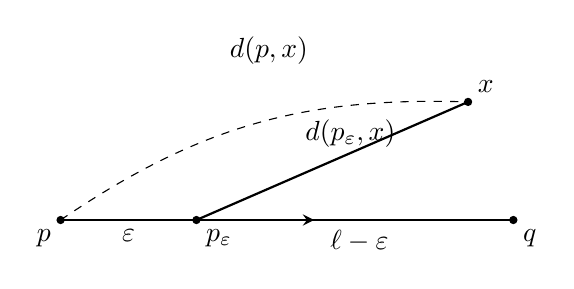
\begin{tikzpicture}[x=1.15cm,y=1cm,>=stealth]
	\coordinate (p) at (0,0);
	\coordinate (e) at (1.5,0);
	\coordinate (q) at (5,0);
	\coordinate (x) at (4.5,1.5);
	\draw[thick] (p)--(q);
	\draw[thick,->] (1.9,0)--(2.8,0);
	\draw[dashed] (p) to[bend left=18] (x);
	\draw[thick] (e)--(x);
	\node[above] at (2.3,1.85) {\(d(p,x)\)};
	\node[above,sloped] at (3.2,.8) {\(d(p_\varepsilon,x)\)};
	\node[below] at (.75,0) {\(\varepsilon\)};
	\node[below] at (3.3,0) {\(\ell-\varepsilon\)};
	\foreach \a in {p,e,q,x} {\fill (\a) circle (1.5pt);}
	\node[below left] at (p) {\(p\)};
	\node[below right] at (e) {\(p_\varepsilon\)};
	\node[below right] at (q) {\(q\)};
	\node[above right] at (x) {\(x\)};
\end{tikzpicture}

	\caption[移动基点构造距离的上支撑]{沿一条最短线把基点从 \(p\) 移到 \(p_\varepsilon\)。从 \(p\) 经 \(p_\varepsilon\) 到 \(x\) 的路线给出 \(r(x)\le\varepsilon+d(p_\varepsilon,x)\)，在 \(q\) 处取等号。图中的直线和弧线仅示意连接关系。}
	\label{g3:fig:distance-support}
\end{figure}

为准确说明“在割点仍成立”，暂记 \(L=\operatorname{div}\operatorname{grad}=-\Delta\)。若连续函数 \(f\) 在 \(q\) 附近满足：对每个 \(\eta>0\)，都有光滑函数 \(h\ge f\)，使 \(h(q)=f(q)\) 且 \(Lh(q)\le b+\eta\)，就称 \(Lf(q)\le b\) 在\term[shangzhicheng yiyi]{上支撑意义}[upper support sense]下成立，也称为相应的\term[pingzhang yiyi]{屏障意义}[barrier sense]。Hessian 的上支撑比较类似定义，以双线性型不等式 \(\operatorname{Hess}h(q)\le B+\eta g_q\) 代替迹不等式。支撑函数只需在 \(q\) 的一个邻域定义，邻域可以随 \(\eta\) 改变。

\begin{theorem}\label{g3:thm:distance-barrier-comparison}
	记 \(L=\operatorname{div}_g\operatorname{grad}_g\)、\(\Delta=-L\)，即采用非负 Laplace 算子约定。
	对给定 \(k\in\mathbb R\)，记 \(s_k\) 为满足 \(s_k''+ks_k=0\)、\(s_k(0)=0\)、\(s_k'(0)=1\) 的模型函数，\(b_k=\pi/\sqrt k\)（\(k>0\)）或 \(b_k=\infty\)（\(k\le0\)），\(\operatorname{ct}_k=s_k'/s_k\) 于 \((0,b_k)\)。
	设 \((M^n,g)\) 连通、完备、光滑且无边界，\(n\ge2\)，\(p\in M\)，\(r=d(p,\cdot)\)，\(k\in\mathbb R\)。若 \(\operatorname{Ric}\ge(n-1)kg\)，则在 \(0<r(q)<b_k\) 的每一点，包括割点，
	\[
		Lr(q)\le(n-1)\operatorname{ct}_k(r(q))
	\]
	在上支撑意义下成立；按本书符号，这就是相应的 \(\Delta r\ge-(n-1)\operatorname{ct}_k(r)\) 屏障估计。若更强地有截面曲率 \(K\ge k\)，选任一从 \(p\) 到 \(q\) 的单位速最短线的末速度 \(v\)，还得到上支撑意义下
	\[
		\operatorname{Hess}r(q)\le\operatorname{ct}_k(r(q))
		\bigl(g_q-v^\flat\otimes v^\flat\bigr).
	\]
\end{theorem}
\begin{proof}
	记 \(\ell=r(q)\)，应用上一引理。\(q\) 距新基点 \(p_\varepsilon\) 为 \(\ell-\varepsilon\)，且在其割迹之外。\cref{g3:thm:laplacian-comparison}给出
	\[
		Lr_\varepsilon(q)\le(n-1)\operatorname{ct}_k(\ell-\varepsilon).
	\]
	因为 \(0<\ell<b_k\)，右边在 \(\varepsilon\downarrow0\) 时趋于 \((n-1)\operatorname{ct}_k(\ell)\)。对给定 \(\eta>0\) 选足够小的 \(\varepsilon\)，即可得到定义要求的上支撑函数。截面曲率下界时，\cref{g3:thm:hessian-comparison}同样给出
	\[
		\operatorname{Hess}r_\varepsilon(q)
		\le\operatorname{ct}_k(\ell-\varepsilon)
		\bigl(g_q-v^\flat\otimes v^\flat\bigr).
	\]
	张量 \(g_q-v^\flat\otimes v^\flat\) 的算子范数为1，故系数的收敛也给出任意小的 \(\eta g_q\) 误差。
\end{proof}

这个构造在 \(\Delta=-L\) 的约定下仍使用距离的上支撑，而支撑函数的 \(\Delta\) 满足下界。它也给出一个便于辨认方向的测试：若光滑 \(\psi\le r\) 在 \(q\) 与 \(r\) 接触，则 \(\psi\le r_\varepsilon\) 且接触值相同，故 \(L\psi(q)\le Lr_\varepsilon(q)\)；取极限得到同一个上界。相反，截面曲率上界所给的光滑区域 Hessian 下界一般不能穿过割迹，因为割迹处的折角可能向下。

\subsection{分布意义下的 Laplace 比较}
\label{g3:subsec:0704:03}

屏障估计是逐点的接触陈述。积分论证还需要分布意义：把可能不光滑的函数与光滑紧支测试函数配对，将导数移到测试函数上。这里直接处理距离函数所需的情形。

\begin{lemma}\label{g3:lem:lipschitz-weak-gradient}
	记 \(L=\operatorname{div}_g\operatorname{grad}_g\)、\(\Delta=-L\)，即采用非负 Laplace 算子约定。
	设 \((M,g)\) 为光滑无边界黎曼流形，\(U\subset M\) 开，\(f:U\to\mathbb R\) 局部 Lipschitz，并在某个闭零测集 \(Z\) 之外光滑。则 \(f\) 的弱梯度由 \(U\setminus Z\) 上的经典梯度几乎处处给出。具体地，对任意光滑紧支向量场 \(X\) 及任意 \(\phi\in C_c^\infty(U)\)，
	\[
		\int_U f\operatorname{div}X\,\mu_g
		=-\int_U\langle\nabla f,X\rangle\,\mu_g,
		\qquad
		\int_U f\Delta\phi\,\mu_g
		=\int_U\langle\nabla f,\nabla\phi\rangle\,\mu_g.
	\]
\end{lemma}
\begin{proof}
	在相对紧坐标盒中，黎曼距离和坐标 Euclid 距离局部互相控制，因此 \(f\) 在坐标中也 Lipschitz。固定除 \(x^i\) 外的坐标，所得一元函数 Lipschitz，因而绝对连续：不交小区间上的函数增量绝对值之和至多为 Lipschitz 常数乘总长度。绝对连续函数的微积分基本定理给出该直线上的积分分部公式，其导数几乎处处存在且有界。

	由 Fubini，几乎每条坐标直线与 \(Z\) 相交于一维零测集。在其余点，刚才的一元导数等于光滑函数的 \(\partial_i f\)。再次用 Fubini，对紧支光滑 \(a\) 有
	\[
		\int f\,\partial_i a\,\mathrm{d}x
		=-\int (\partial_i f)a\,\mathrm{d}x.
	\]
	在此式中取 \(a=\sqrt{\det G}\,X^i\)，求和并使用第一章的散度坐标公式，便得坐标盒内的第一个等式。用有限个从属坐标片的光滑权重分解 \(X\)，额外的权重导数因和为1而相消，得到全局式。最后取 \(X=\nabla\phi\)，再用 \(\Delta=-\operatorname{div}\nabla\)，即得第二个等式。
\end{proof}

对局部可积的 \(f\)，定义分布 \(\Delta f\) 在测试函数 \(\phi\) 上的值为 \(\int f\Delta\phi\,\mu_g\)。若对每个非负 \(\phi\in C_c^\infty(U)\) 都有
\[
	\int_U f\Delta\phi\,\mu_g\ge\int_U b\phi\,\mu_g,
\]
就称 \(\Delta f\ge b\) 在\term[fenbu yiyi]{分布意义}[distributional sense]下成立。上一引理把这个定义转化为一阶导数的积分，因而可以用于1-Lipschitz 的距离函数。非负测试函数和不等式方向都是定义的一部分。

\begin{theorem}\label{g3:thm:distributional-laplacian-comparison}
	记 \(L=\operatorname{div}_g\operatorname{grad}_g\)、\(\Delta=-L\)，即采用非负 Laplace 算子约定。
	对给定 \(k\in\mathbb R\)，记 \(s_k\) 为满足 \(s_k''+ks_k=0\)、\(s_k(0)=0\)、\(s_k'(0)=1\) 的模型函数，\(b_k=\pi/\sqrt k\)（\(k>0\)）或 \(b_k=\infty\)（\(k\le0\)），\(\operatorname{ct}_k=s_k'/s_k\) 于 \((0,b_k)\)。
	设 \((M^n,g)\) 连通、完备、光滑且无边界，\(n\ge2\)，\(\operatorname{Ric}\ge(n-1)kg\)，\(p\in M\)。令 \(r=d(p,\cdot)\)、\(U_k=\{x:0<r(x)<b_k\}\)。则在 \(U_k\) 上
	\begin{equation}\label{g3:eq:distributional-laplacian-comparison}
		\Delta r\ge-(n-1)\operatorname{ct}_k(r)
	\end{equation}
	在分布意义下成立。等价地，对每个非负 \(\phi\in C_c^\infty(U_k)\)，
	\[
		\int_{U_k}\langle\nabla r,\nabla\phi\rangle\,\mu_g
		\ge-\int_{U_k}(n-1)\operatorname{ct}_k(r)\phi\,\mu_g.
	\]
\end{theorem}
\begin{proof}
	距离为1-Lipschitz，且在闭零测集 \(\{p\}\cup\operatorname{Cut}(p)\) 外光滑，故上一引理适用。取 \(0<a<R<b_k\)，使 \(\phi\) 的支集包含于 \(\{a<r<R\}\)，并把 \(R\) 取得严格大于支集上的最大距离。在式\eqref{g3:eq:polar-cut-integration}中写
	\[
		\Phi(t,u)=\phi(\exp_p(tu)),\qquad
		\tau(u)=\min\{c_p(u),R\}.
	\]
	当 \(0<t<c_p(u)\) 时，\(\nabla r=\partial_t\)，所以
	\[
		\int\langle\nabla r,\nabla\phi\rangle\,\mu_g
		=\int_{S_pM}\int_0^{\tau(u)}\partial_t\Phi\,\theta\,\mathrm{d}t\,\mathrm{d}\sigma(u).
	\]
	对每条射线作一元分部积分。起端项为零，因为 \(\Phi=0\) 于支集以前；末端在 \(\tau=R\) 时同样为零，在有限割时 \(\tau=c_p(u)<R\) 时为
	\(\Phi(c_p(u),u)\theta(c_p(u),u)\ge0\)。这里 \(A_u\) 光滑延拓至割时，\(\theta\) 从正值趋于非负值；若该端点共轭，行列式就是零。因此
	\begin{equation}\label{g3:eq:cut-boundary-flux}
		\int\langle\nabla r,\nabla\phi\rangle\,\mu_g
		=\mathcal B_p(\phi)-\int_{S_pM}\int_0^{\tau(u)}\Phi\,\partial_t\theta\,\mathrm{d}t\,\mathrm{d}\sigma,
		\qquad \mathcal B_p(\phi)\ge0.
	\end{equation}
	这些积分和端点极限可以按方向积分：在紧集 \(S_pM\times[0,R]\) 上，Jacobi 方程的光滑依赖给出 \(\theta\)、\(\partial_t\theta\) 的共同界，而 \(c_p\) 可测，测试函数又有紧支集。

	在割时之前，由\cref{g3:thm:riccati-trace-comparison}和行列式求导，
	\[
		\partial_t\theta=h\theta
		\le(n-1)\operatorname{ct}_k(t)\theta.
	\]
	由于 \(\Phi\ge0\)，将此式代入 \eqref{g3:eq:cut-boundary-flux}并保留非负末端项，得到
	\[
		\int\langle\nabla r,\nabla\phi\rangle\,\mu_g
		\ge-\int_{S_pM}\int_0^{\tau(u)}
		(n-1)\operatorname{ct}_k(t)\Phi\theta\,\mathrm{d}t\,\mathrm{d}\sigma.
	\]
	再用极坐标换元，右端就是所要求的积分。这个证明同时说明：割迹的贡献在 \(Lr\) 中为非正，在本书的 \(\Delta r\) 中为非负。
\end{proof}

常曲率的逐点公式不能照搬为越过割迹的分布等式。例如平坦圆柱上，距离在一条割线上由两支光滑函数取较小者；两支的一阶导数在那里发生向下跳跃。因此即使所有光滑点都满足模型等式，分布中仍会多出割线项。章末习题将计算这一项。

\subsection{等号传播及局部空间形式}
\label{g3:subsec:0704:04}

比较中的等号记录了证明里各个非负量同时消失。Rauch 比较的单一方向等号控制一条 Jacobi 场；Ricci 迹比较的等号还使径向形算子各特征值相同。只有在一族方向上获得这些信息，才会确定一个开区域的度量。

\begin{proposition}\label{g3:prop:radial-metric-evolution}
	将法向空间沿线平行识别，径向 Jacobi 张量 \(A\) 满足 \(A''+\mathcal RA=0\)、\(A(0)=0\)、\(A'(0)=I\)，其中 \(\mathcal R=R(\cdot,\dot\gamma)\dot\gamma\)；在 \(A\) 可逆处记 \(S=A'A^{-1}\)、\(h=\operatorname{tr}S\)，\(I\) 为恒等算子。
	沿所述测地线，\(T=\dot\gamma\)，\(R\) 表示 Levi-Civita 曲率，\(P\) 表示沿线平行移动，撇号表示协变导数。
	对给定 \(k\in\mathbb R\)，记 \(s_k\) 为满足 \(s_k''+ks_k=0\)、\(s_k(0)=0\)、\(s_k'(0)=1\) 的模型函数，\(b_k=\pi/\sqrt k\)（\(k>0\)）或 \(b_k=\infty\)（\(k\le0\)），\(\operatorname{ct}_k=s_k'/s_k\) 于 \((0,b_k)\)。
	设 \((M^n,g)\) 为光滑无边界黎曼流形，\(p\in M\)，且 \(\exp_p\) 在切球 \(B_R(0)\) 上为微分同胚。令 \(F(t,u)=\exp_p(tu)\)，\(0<t<R\)、\(u\in S_pM\)。则
	\[
		F^*g=\mathrm{d}t^2+G_t,
	\]
	其中 \(G_t\) 是单位切球面上的度量族。若沿每条射线有 \(S(t)=\operatorname{ct}_k(t)I\)，且 \(R\le b_k\)，则
	\begin{equation}\label{g3:eq:model-polar-metric-rigidity}
		G_t=s_k(t)^2g_{S_pM}.
	\end{equation}
\end{proposition}
\begin{proof}
	Gauss 引理给出径向与角向的正交分解。对 \(u^\perp=\mathrm{T}_uS_pM\) 中的 \(a,b\)，令 \(J_a,J_b\) 为对应角向 Jacobi 场，则
	\[
		G_t(a,b)=\langle J_a(t),J_b(t)\rangle.
	\]
	径向形算子满足 \(J_a'=SJ_a\)，故
	\[
		\partial_tG_t(a,b)
		=\langle SJ_a,J_b\rangle+\langle J_a,SJ_b\rangle.
	\]
	当 \(S=\operatorname{ct}_k I\) 时，右端为 \(2\operatorname{ct}_kG_t(a,b)\)，于是 \(\partial_t(s_k^{-2}G_t)=0\)。另一方面，\(J_a(t)=tP_ta+O(t^3)\)、\(s_k(t)/t\to1\)，因此 \(s_k(t)^{-2}G_t(a,b)\to\langle a,b\rangle\)。常数只能是单位切球面的标准度量，得到式\eqref{g3:eq:model-polar-metric-rigidity}。
\end{proof}

\begin{theorem}\label{g3:thm:laplacian-equality-local-space-form}
	记 \(L=\operatorname{div}_g\operatorname{grad}_g\)、\(\Delta=-L\)，即采用非负 Laplace 算子约定。
	对给定 \(k\in\mathbb R\)，记 \(s_k\) 为满足 \(s_k''+ks_k=0\)、\(s_k(0)=0\)、\(s_k'(0)=1\) 的模型函数，\(b_k=\pi/\sqrt k\)（\(k>0\)）或 \(b_k=\infty\)（\(k\le0\)），\(\operatorname{ct}_k=s_k'/s_k\) 于 \((0,b_k)\)。
	设 \((M^n,g)\) 连通、完备、光滑且无边界，\(n\ge2\)，\(\operatorname{Ric}\ge(n-1)kg\)，\(p\in M\)，\(r=d(p,\cdot)\)。设 \(0<R<\min\{\operatorname{inj}_g(p),b_k\}\)。若对每个 \(u\in S_pM\)，在 \(q=\exp_p(Ru)\) 处都有
	\[
		\Delta r(q)=-(n-1)\operatorname{ct}_k(R),
	\]
	则 \(B(p,R)\) 与常截面曲率 \(k\) 的标准模型中半径 \(R\) 的球等距，且等距可取为指定起点切空间线性等距所诱导的指数坐标对应。
\end{theorem}
\begin{proof}
	沿任意固定方向 \(u\)，所给等号就是 \(h(R)=(n-1)\operatorname{ct}_k(R)\)。由\cref{g3:prop:riccati-trace-rigidity}，该方向上全部 \(0<t\le R\) 满足 \(S=\operatorname{ct}_k I\)。其证明中的等号分别使 \(\operatorname{Ric}(T,T)=(n-1)k\) 和无迹部分 \(S-hI/(n-1)\) 为零；因此得到的是整个径向算子的结论。对所有方向应用上一命题，便有
	\[
		F^*g=\mathrm{d}t^2+s_k(t)^2g_{S_pM}.
	\]
	在标准常曲率模型上，\cref{g3:exm:constant-curvature-jacobi}给出同样的角向 Jacobi 场和同样的极坐标度量。任选两起点切空间间的线性等距，先在切球中对应向量，再分别使用指数映射，就得到穿孔球上的等距。该对应本身在中心光滑，其微分为所选线性等距，所以由度量的连续性，中心处也保持度量。\(R\) 小于两侧的指数单射半径，故该对应是整个球的微分同胚与等距。
\end{proof}

这里只需在整张半径 \(R\) 的测地球面上取得迹等号，就能沿各射线向内恢复整个球的度量。若只在一个方向取得等号，结论相应限于这一条射线；若只知道一支 Jacobi 场的长度达到 Rauch 等号，控制的方向还要更少。下一章将把径向密度的不等式沿方向积分，得到球体积比较，并继续分析整体几何受到的限制。
% 纲要条目排为编号小节标题，并进入目录与书签；说明段仍保留于纲要注释中。


\begin{chaptersummary}
	指标形式的端点极小性给出曲率与径向伸缩的比较，积分后便是 Rauch 长度估计。较大的截面曲率使共同初始导数的法向 Jacobi 场受到更强的约束；比较必须在模型函数为正并满足所需非共轭条件的区间内进行。指数映射微分的估计是局部长度信息，不能单独保证全局单射或最短性。

	\ProseParagraphBreak

	矩阵 \(S=A'A^{-1}\) 同时描述 Jacobi 场的相对增长和测地球面的径向变化。Riccati 方程取迹后，\(\operatorname{tr}S^2\ge(\operatorname{tr}S)^2/(n-1)\) 把 Ricci 下界变为迹上界；无迹部分是否消失决定了等号。距离 Hessian 是这个算子的几何表达，极坐标密度的对数导数则是它的迹。

	\ProseParagraphBreak

	割迹外的光滑比较可用移动基点延伸为上支撑估计，也可用极坐标分部积分延伸为分布不等式；后者保留了割点处符号确定的边界贡献。等号先沿射线向内传播，若整张测地球面的迹都达到模型值，就能恢复球内的极坐标度量。下一章将进一步沿方向和半径积分，研究体积、直径与整体拓扑约束。
\end{chaptersummary}

\BookExercises

\begin{exercise}\label{g3:ex:rauch-equality-single-geodesic}
	在 \(M=\mathbb R\times S^2(a)\) 上取乘积度量，固定 \(p=(0,q)\)，令 \(u\) 为实直线因子的正向单位向量，\(\gamma(t)=(t,q)\)。
	\begin{enumerate}
		\item 证明 \(M\) 的截面曲率非负，但沿 \(\gamma\) 的每个径向截面曲率都为零。
		\item 求沿 \(\gamma\) 满足 \(J(0)=0\) 的所有 Jacobi 场，并证明对每个 \(t>0\)，\((\mathrm d\exp_p)_{tu}\) 都是线性等距。
		\item 证明 \(\gamma\) 的任一点都没有与 Euclid 空间局部等距的邻域。由此说明，在一条固定的径向测地线上，所有初始法向方向都达到 Rauch 平坦模型的等号，仍不足以确定邻域的度量。
	\end{enumerate}
\end{exercise}
\begin{solution}
	设 \(X=(x,X_S)\)、\(Y=(y,Y_S)\) 为乘积中的切向量。由\cref{g3:prop:product-curvature}，
	\[
		\langle R(X,Y)Y,X\rangle
		=\frac1{a^2}\bigl(|X_S|^2|Y_S|^2-\langle X_S,Y_S\rangle^2\bigr)\ge0.
	\]
	若 \(X=u\)，其球面分量为零，曲率分子为零；故含 \(u\) 的每个截面曲率均为零。事实上，乘积曲率公式还给出 \(R(V,u)u=0\) 对任意 \(V\) 成立。

	于是沿 \(\gamma\) 的 Jacobi 方程为 \(J''=0\)。若 \(P_t\) 为从 \(0\) 到 \(t\) 的平行移动，所有初始值为零的解恰为
	\[
		J_w(t)=tP_tw,\qquad w\in \mathrm{T}_pM.
	\]
	由指数映射的微分公式，
	\[
		(\mathrm d\exp_p)_{tu}(w)=\frac1tJ_w(t)=P_tw,
	\]
	所以微分是线性等距。这也说明沿该线无共轭时刻。

	另一方面，每点的球面因子切平面都有截面曲率 \(a^{-2}>0\)。局部等距保持曲率，而 Euclid 空间所有截面曲率为零，因此任一点附近都不可能与 Euclid 空间局部等距。该例在固定的一条径向线上取等号，却没有在从 \(p\) 出发的一个开集方向上给出同样信息；邻域刚性需要这样的额外方向条件。
\end{solution}

\begin{exercise}\label{g3:ex:normal-coordinate-bilipschitz}
	设 \((M,g)\) 为光滑无边界黎曼流形，\(p\in M\)，\(\kappa>0\)，且 \(0<\rho<\pi/\sqrt\kappa\)。假设 \(\exp_p\) 把切空间开球 \(B(0,\rho)\) 微分同胚地映到 \(U\)，并且每条从 \(p\) 出发、参数小于 \(\rho\) 的径向测地线上的径向截面曲率都满足 \(-\kappa\le K\le\kappa\)。令
	\[
		\alpha=\frac{\sin(\sqrt\kappa\,\rho)}{\sqrt\kappa\,\rho},
		\qquad
		\beta=\frac{\sinh(\sqrt\kappa\,\rho)}{\sqrt\kappa\,\rho}.
	\]
	证明法坐标中的拉回度量满足
	\[
		\alpha^2|\xi|^2
		\le (\exp_p^*g)_v(\xi,\xi)
		\le\beta^2|\xi|^2
		\qquad(v\in B(0,\rho),\ \xi\in \mathrm{T}_pM).
	\]
	记 \(d_U\) 为只允许曲线留在 \(U\) 内所定义的路径距离。进一步证明
	\[
		\alpha|v-w|
		\le d_U(\exp_pv,\exp_pw)
		\le\beta|v-w|.
	\]
	说明为何一般不能直接把中间的 \(d_U\) 换成 \(M\) 的距离，以及强凸性为何足以允许这种替换。
\end{exercise}
\begin{solution}
	设 \(v=ru\ne0\)、\(|u|=1\)，写 \(\xi=bu+z\)、\(z\perp u\)。由\cref{g3:prop:exponential-length-comparison}的双边形式，
	\[
		b^2+\left(\frac{s_\kappa(r)}r\right)^2|z|^2
		\le(\exp_p^*g)_v(\xi,\xi)
		\le b^2+\left(\frac{s_{-\kappa}(r)}r\right)^2|z|^2.
	\]
	其中曲率上界先保证 \(r<\pi/\sqrt\kappa\) 时没有共轭点，故两个方向均可用。

	为取得整个坐标球上的常数，注意
	\[
		\frac{\mathrm d}{\mathrm dr}\frac{s_k(r)}r
		=\frac1{r^2}\int_0^r\bigl(c_k(r)-c_k(t)\bigr)\,\mathrm dt.
	\]
	在 \((0,\pi/\sqrt\kappa)\) 上，\(c_\kappa(t)=\cos(\sqrt\kappa\,t)\) 递减，故 \(s_\kappa(r)/r\) 递减；\(c_{-\kappa}(t)=\cosh(\sqrt\kappa\,t)\) 递增，故 \(s_{-\kappa}(r)/r\) 递增。二者在 \(0\) 的极限都为 \(1\)，因而
	\[
		0<\alpha\le\frac{s_\kappa(r)}r\le1
		\le\frac{s_{-\kappa}(r)}r\le\beta.
	\]
	代入即可得到度量估计，在 \(v=0\) 处由 \((\mathrm d\exp_p)_0=I\) 成立。

	任取 \(U\) 中连接 \(\exp_pv\) 与 \(\exp_pw\) 的分段光滑曲线，拉回为球中的曲线 \(c\)，度量下界给出
	\[
		\operatorname{Len}_g(\exp_p\circ c)
		\ge\alpha\operatorname{Len}_{g_p}(c)
		\ge\alpha|v-w|.
	\]
	取下确界得到距离下界。为得上界，用切空间中的直线段连接 \(v,w\)；开球凸，所以整段仍在球内。度量上界给出其像的长度至多为 \(\beta|v-w|\)。

	流形距离允许连接曲线离开 \(U\)，因此一般只有 \(d_M\le d_U\)，上述下界不能自动传给 \(d_M\)。如果 \(U\) 强凸，每对点之间的全局最短测地线都留在 \(U\)，故 \(d_M=d_U\)，两边的估计便同时成立。
\end{solution}

\begin{exercise}\label{g3:ex:first-conjugate-upper-bound-rigidity}
	取 \(k\in\mathbb R\)。记 \(s_k\) 为 \(s_k''+ks_k=0\)、\(s_k(0)=0\)、\(s_k'(0)=1\) 的解，\(c_k=s_k'\)、\(\operatorname{ct}_k=c_k/s_k\)，\(b_k=\pi/\sqrt k\) 当 \(k>0\)，否则 \(b_k=\infty\)。
	设 \(\gamma:[0,b_k]\to M\) 是 \(n\ge2\) 维光滑无边界黎曼流形中的单位速测地线，延拓到端点邻域，其中 \(k>0\)、\(b_k=\pi/\sqrt k\)。假设沿线每个径向截面满足 \(K\ge k\)。证明以下两项等价：
	\begin{enumerate}
		\item 相对起点的第一个正共轭时刻恰为 \(b_k\)。
		\item 在 \(0\le t\le b_k\) 上，对所有 \(V\perp\dot\gamma(t)\) 都有 \(R(V,\dot\gamma)\dot\gamma=kV\)。
	\end{enumerate}
	证明此时 \(b_k\) 处的共轭重数为 \(n-1\)。进一步说明，若某个内时刻存在径向截面曲率严格大于 \(k\)，则首共轭时刻必严格小于 \(b_k\)。提示：使用首个共轭端点处指标形式的半正定性，以及两端为零的模型试探场。
\end{exercise}
\begin{solution}
	先假设第一个正共轭时刻为 \(b_k\)。取任意平行单位法向场 \(E\)，令 \(V(t)=s_k(t)E(t)\)。由于 \(s_k(0)=s_k(b_k)=0\)，场 \(V\) 两端为零。\cref{g3:prop:first-conjugate-semidefinite}给出 \(I_\gamma(V)\ge0\)，而曲率下界给出
	\[
		I_\gamma(V)\le I_k(V)
		=\int_0^{b_k}\bigl((s_k')^2-ks_k^2\bigr)\,\mathrm dt
		=[s_ks_k']_0^{b_k}=0.
	\]
	因此两个指标值都为零，且
	\[
		0=I_k(V)-I_\gamma(V)
		=\int_0^{b_k}s_k(t)^2
		\bigl(\langle R(E,T)T,E\rangle-k\bigr)\,\mathrm dt.
	\]
	被积函数连续、非负，而 \(s_k>0\) 于内部，故 \(\langle R(E,T)T,E\rangle=k\) 在整个内部成立，在端点由连续性成立。任一时刻的任意单位法向量都可平行延拓成这样的 \(E\)，所以曲率算子的二次型在法空间上恒为 \(k|V|^2\)。算子自伴，由极化便得到 \(R(V,T)T=kV\)。

	反过来，若第二项成立，所有法向零初值 Jacobi 场都为
	\[
		J_w(t)=s_k(t)P_{t\leftarrow0}w,
		\qquad w\perp T(0).
	\]
	它们在 \(0<t<b_k\) 处没有非零场消失，在 \(b_k\) 处则全部消失。切向零初值解为 \(atT\)，在正时刻不能再次消失，除非 \(a=0\)。因此首共轭时刻正是 \(b_k\)，重数为法空间维数 \(n-1\)。

	最后，\cref{g3:prop:conjugate-radius-comparison}已经保证首共轭时刻不超过 \(b_k\)。若在某个内时刻有径向截面曲率严格大于 \(k\)，第二项不成立，刚证的等价性排除首时刻等于 \(b_k\)，故必严格小于 \(b_k\)。
\end{solution}

\begin{exercise}\label{g3:ex:riccati-higher-radial-expansion}
	设 \((M^n,g)\) 为光滑无边界黎曼流形，\(n\ge2\)，\(\gamma(t)=\exp_p(tv)\) 为单位速测地线，\(m=n-1\)。记 \(\mathcal R=R(\cdot,\dot\gamma)\dot\gamma\) 为法向曲率算子，\(A\) 为满足 \(A(0)=0,A'(0)=I\) 的径向 Jacobi 张量，\(S=A'A^{-1}\)、\(\theta=\det A\)。在沿线平行标架中记 \(\mathcal R_0=\mathcal R(0)\)、\(\mathcal R_1=\mathcal R'(0)\)。将式\eqref{g3:eq:radial-riccati-initial}再展开一阶，求 \(A(t)\) 的四次项、\(S(t)\) 的二次项以及 \(\theta(t)/t^m\) 的三次项。说明把初始方向 \(v\) 改为 \(-v\) 时，最后一个三次项怎样变化。
\end{exercise}
\begin{solution}
	对 \(A''=-\mathcal R A\) 连续求导并在零处代入 \(A(0)=0\)、\(A'(0)=\operatorname{id}\)，得到
	\[
		A''(0)=0,\qquad A'''(0)=-\mathcal R_0,\qquad A^{(4)}(0)=-2\mathcal R_1.
	\]
	所以光滑性和 Taylor 定理给出
	\[
		\begin{aligned}
		A(t)&=t\operatorname{id}-\frac{t^3}{6}\mathcal R_0-\frac{t^4}{12}\mathcal R_1+O(t^5),\\
		A'(t)&=\operatorname{id}-\frac{t^2}{2}\mathcal R_0-\frac{t^3}{3}\mathcal R_1+O(t^4),\\
		A(t)^{-1}&=t^{-1}\left(\operatorname{id}+\frac{t^2}{6}\mathcal R_0+\frac{t^3}{12}\mathcal R_1+O(t^4)\right).
		\end{aligned}
	\]
	将后两式相乘，二次以上的小矩阵相互乘积只影响 \(S\) 的三次及更高次项，故
	\[
		S(t)=t^{-1}\operatorname{id}-\frac t3\mathcal R_0-\frac{t^2}{4}\mathcal R_1+O(t^3).
	\]
	另一方面，\(\det(\operatorname{id}+X)=1+\operatorname{tr}X+O(\lVert X\rVert^2)\)，且此处 \(X=O(t^2)\)。因此
	\[
		\frac{\theta(t)}{t^m}
		=1-\frac{t^2}{6}\operatorname{Ric}_p(v,v)
		-\frac{t^3}{12}(\nabla_v\operatorname{Ric})_p(v,v)+O(t^4).
	\]
	迹与沿线协变导数可交换，而 \(v\) 沿测地线平行，这说明 \(\operatorname{tr}\mathcal R_1=(\nabla_v\operatorname{Ric})(v,v)\)。反向射线的 \(\operatorname{Ric}_p(-v,-v)=\operatorname{Ric}_p(v,v)\)，但
	\((\nabla_{-v}\operatorname{Ric})_p(-v,-v)=-(\nabla_v\operatorname{Ric})_p(v,v)\)，故二次项不变、三次项变号。点处密度在相反方向的首个可能差异出现在这一奇次项。
\end{solution}

\begin{exercise}\label{g3:ex:product-strict-trace-comparison}
	在乘积 \(M=\mathbb H^2(-a^2)\times\mathbb R\) 上取乘积度量，其中 \(a>0\)，第一因子的常曲率为 \(-a^2\)。设单位速测地线 \(\gamma\) 完全沿第一因子行走。求它的法向径向 Jacobi 张量 \(A\)、\(S=A'A^{-1}\)、\(h=\operatorname{tr}S\) 和密度 \(\theta=\det A\)。用迹比较说明，对每个 \(t>0\)，
	\[
		a\coth(at)+\frac1t<\sqrt2\,a\coth\left(\frac{at}{\sqrt2}\right),
		\qquad
		\frac{t\sinh(at)}a<\frac2{a^2}\sinh^2\left(\frac{at}{\sqrt2}\right).
	\]
	解释为什么沿线 \(\operatorname{Ric}(T,T)\) 恰好等于模型下界，比较却仍严格。
\end{exercise}
\begin{solution}
	取第一因子中与 \(T\) 垂直的平行单位场 \(E_1\)，以及第二因子的单位场 \(E_2\)。\cref{g3:prop:product-curvature}的乘积曲率公式给出
	\(\mathcal R=\operatorname{diag}(-a^2,0)\)。分别解两个标量 Jacobi 初值问题，得到
	\[
		A(t)=\begin{pmatrix}\sinh(at)/a&0\\0&t\end{pmatrix},\qquad
		S(t)=\begin{pmatrix}a\coth(at)&0\\0&1/t\end{pmatrix}.
	\]
	于是
	\[
		h(t)=a\coth(at)+\frac1t,\qquad
		\theta(t)=\frac{t\sinh(at)}a.
	\]
	两项分离量对 \(t>0\) 都不为零，故不存在正共轭时刻。这里 \(m=2\)、\(\operatorname{Ric}(T,T)=-a^2=mk\)，应选 \(k=-a^2/2\)。模型迹与密度正是题设两个右端，\cref{g3:thm:riccati-trace-comparison,g3:prop:radial-density-comparison}给出不严格比较。

	对 \(x>0\)，函数 \(x\cosh x-\sinh x\) 在零处为零，导数为 \(x\sinh x>0\)。因此 \(x\coth x>1\)，从而 \(S\) 的两个特征值始终不相等。式\eqref{g3:eq:riccati-trace-cauchy-schwarz}的差值严格为正。尽管 Ricci 误差项为零，式\eqref{g3:eq:riccati-trace-defect}中的 \(F\) 仍处处为正，故迹比较严格。密度比的对数导数严格为负，且比值在起点趋于一，所以密度比较也严格。这个例子显示，Ricci 等于模型值并不保证各个方向的扩张率相同。
\end{solution}

\begin{exercise}\label{g3:ex:regular-riccati-focusing}
	设 \(m\ge1\)，\(\mathcal R(t)\) 是定义于 \([0,\infty)\) 的光滑实对称 \(m\) 阶矩阵函数，且 \(\operatorname{tr}\mathcal R(t)\ge0\)。设实对称矩阵解 \(S\) 满足
	\[
		S'+S^2+\mathcal R=0,\qquad \operatorname{tr}S(0)=-\alpha<0.
	\]
	证明：\(S\) 不能作为有限光滑矩阵解存在到时刻 \(m/\alpha\)。说明这与径向解在零处的奇异初值问题有何不同，并给出达到这一时间上界的 Euclid 法线聚焦模型。
\end{exercise}
\begin{solution}
	令 \(h=\operatorname{tr}S\)。迹方程与 Cauchy--Schwarz 不等式给出
	\[
		h'=-\operatorname{tr}(S^2)-\operatorname{tr}\mathcal R
		\le-\frac{h^2}{m}.
	\]
	因此 \(h\) 不增，始终不大于 \(-\alpha\)，可以取倒数。对存在区间内的每个 \(t\ge0\)，有
	\[
		\left(\frac1h\right)'=-\frac{h'}{h^2}\ge\frac1m,
		\qquad
		\frac1{h(t)}\ge-\frac1\alpha+\frac tm.
	\]
	若有限矩阵解存在到 \(t=m/\alpha\)，右端非负，而左端严格为负，矛盾。对 \(0\le t<m/\alpha\) 还可写为
	\[
		h(t)\le-\frac{\alpha}{1-\alpha t/m}.
	\]
	为解释有限端点处的发散，取线性系统 \(A''+\mathcal R A=0\)、\(A(0)=\operatorname{id}\)、\(A'(0)=S(0)\) 的全区间解；其存在性由\cref{g3:thm:jacobi-initial-data}证明中的线性系统方法得到。在 \(S\) 的存在区间内，令 \(Z=A'-SA\)，则 \(Z'=-SZ\)、\(Z(0)=0\)，故 \(A'=SA\) 且 \(\det A(t)=\exp(\int_0^t h)\)。若最大存在区间右端 \(\tau\) 有限而 \(S\) 有界，则该行列式在 \(\tau\) 仍有正的极限，所以 \(A'A^{-1}\) 在 \(\tau\) 附近光滑并延拓 \(S\)，矛盾。因此有限端点确实伴随矩阵失去有界性。

	令 \(b=m/\alpha\)，取 \(\mathcal R=0\)、\(S(t)=-(b-t)^{-1}\operatorname{id}\)，则方程成立，初始迹为 \(-m/b=-\alpha\)，并恰在 \(b\) 处爆破。它是 \(\mathbb R^{m+1}\) 中半径 \(b\) 球面的内法线族：沿法线的切向分离张量为
	\(A(t)=(1-t/b)\operatorname{id}\)，在球心同时消失。这里初始截面是一个具有有限形算子的超曲面，\(S(0)=-b^{-1}\operatorname{id}\) 有限；从单点发出的径向族则有 \(A(0)=0\)、\(S(t)\sim t^{-1}\operatorname{id}\)，不能把本题的有限初值直接放到那个奇异起点上。
\end{solution}

\begin{exercise}\label{g3:ex:model-radial-potential}
	取 \(k\in\mathbb R\)。记 \(s_k\) 为 \(s_k''+ks_k=0\)、\(s_k(0)=0\)、\(s_k'(0)=1\) 的解，\(c_k=s_k'\)、\(\operatorname{ct}_k=c_k/s_k\)，\(b_k=\pi/\sqrt k\) 当 \(k>0\)，否则 \(b_k=\infty\)。
	设 \((M^n,g)\) 为光滑无边界黎曼流形，\(p\in M\)，\(r=d(p,\cdot)\)，\(c_p\) 为割时函数，\(T\) 为单位径向速度。定义
	\[
		\Phi_k(t)=\int_0^t s_k(u)\,\mathrm du.
	\]
	求 \(\Phi_k\) 的显式表达式，证明对任意黎曼流形的局部距离函数 \(r=d(p,\cdot)\)，\(\Phi_k(r)\) 在初点 \(p\) 光滑，且
	\(\operatorname{Hess}\Phi_k(r)|_p=g_p\)。
	在 \(0<r<\min\{c_p(u),b_k\}\) 上，分别从径向截面上界 \(K\le k\)、下界 \(K\ge k\) 推出它的 Hessian 比较；再从径向 Ricci 下界 \(\operatorname{Ric}(T,T)\ge(n-1)k\) 推出本书符号下的 Laplace 比较，并核对常曲率模型中的等号。
\end{exercise}
\begin{solution}
	积分得到
	\[
		\Phi_k(t)=
		\begin{cases}
			(1-\cos(\sqrt{k}t))/k,&k>0,\\
			t^2/2,&k=0,\\
			(\cosh(\sqrt{-k}t)-1)/(-k),&k<0.
		\end{cases}
	\]
	三个表达式在零附近都有收敛的偶次幂展开
	\[
		\Phi_k(t)=\frac{t^2}{2}-\frac{kt^4}{24}+O(t^6).
	\]
	在法坐标中 \(r^2=\sum_i(x^i)^2\)，因此把该收敛级数写成 \(r^2\) 的光滑函数，就得到初点处的光滑性；二次项给出中心 Hessian 为 \(g_p\)。

	因为 \(\Phi_k'=s_k\)、\(\Phi_k''=c_k\)，链式公式给出
	\[
		\operatorname{Hess}\Phi_k(r)
		=c_k(r)\,\mathrm dr\otimes\mathrm dr
		+s_k(r)\operatorname{Hess}r.
	\]
	在 \(0<r<b_k\) 中 \(s_k(r)>0\)，故截面上界给出
	\[
		\operatorname{Hess}\Phi_k(r)
		\ge c_k(r)\,\mathrm dr\otimes\mathrm dr+
		s_k(r)\operatorname{ct}_k(r)
		\bigl(g-\mathrm dr\otimes\mathrm dr\bigr)
		=c_k(r)g.
	\]
	截面下界给出反向不等式。这里乘以的是正数 \(s_k\)，即使 \(k>0\) 且 \(c_k\) 已变负，不等号方向也不改变。

	在 Ricci 下界下，由 \(\Phi_k'=s_k>0\) 得
	\[
		\Delta\Phi_k(r)
		\ge-c_k(r)-(n-1)s_k(r)\operatorname{ct}_k(r)
		=-n c_k(r).
	\]
	常曲率模型中 \(\operatorname{Hess}r=\operatorname{ct}_k(r)(g-\mathrm dr\otimes\mathrm dr)\)，所以
	\(\operatorname{Hess}\Phi_k(r)=c_k(r)g\)、
	\(\Delta\Phi_k(r)=-n c_k(r)\)。
	在初点 \(c_k(0)=1\)，所有公式与中心 Hessian 及 \(\Delta\Phi_k(r)(p)=-n\) 相容。
\end{solution}

\begin{exercise}\label{g3:ex:model-radial-harmonic-comparison}
	取 \(k\in\mathbb R\)。记 \(s_k\) 为 \(s_k''+ks_k=0\)、\(s_k(0)=0\)、\(s_k'(0)=1\) 的解，\(c_k=s_k'\)、\(\operatorname{ct}_k=c_k/s_k\)，\(b_k=\pi/\sqrt k\) 当 \(k>0\)，否则 \(b_k=\infty\)。
	设 \((M^n,g)\) 为光滑无边界黎曼流形，\(p\in M\)，\(r=d(p,\cdot)\)，\(T\) 为单位径向速度，\(\Delta=-\operatorname{div}_g\operatorname{grad}_g\)，\(n\ge2\)、\(0<R<b_k\)，在 \(0<t\le R\) 上定义
	\[
		G_{k,R}(t)=\int_t^R s_k(u)^{-(n-1)}\,\mathrm du.
	\]
	证明在常曲率 \(k\) 的模型中，\(G_{k,R}(r)\) 在相应穿孔球内调和。若一般流形沿从 \(p\) 出发的有关最短径向线满足
	\(\operatorname{Ric}(T,T)\ge(n-1)k\)，证明在
	\(0<r<R\) 且未到割点的范围内，
	\[
		\Delta G_{k,R}(r)\le0.
	\]
	写出 \(k=0\) 时 \(n=2\) 与 \(n>2\) 的表达式，并解释为何这里的不等号与 \(\Delta r\) 的比较方向不同。
\end{exercise}
\begin{solution}
	记 \(m=n-1\)。有
	\[
		G_{k,R}'(t)=-s_k(t)^{-m},\qquad
		G_{k,R}''(t)
		=m\operatorname{ct}_k(t)s_k(t)^{-m}
		=-m\operatorname{ct}_k(t)G_{k,R}'(t).
	\]
	因此它满足模型径向调和方程
	\(G''+m\operatorname{ct}_kG'=0\)。
	模型中 \(Lr=m\operatorname{ct}_k(r)\)，代入径向 Laplace 公式得到 \(\Delta G(r)=0\)。

	一般情形中直接保留导数的符号计算：
	\[
		\Delta G(r)
		=-G''(r)-G'(r)Lr
		=-G'(r)\bigl(Lr-m\operatorname{ct}_k(r)\bigr).
	\]
	由 Ricci 比较，括号不大于零；而 \(-G'>0\)，所以右边不大于零。等价地，这是\cref{g3:prop:radial-function-laplacian}中递减径向函数所用的方向。

	当 \(k=0\) 时，
	\[
		G_{0,R}(t)=
		\begin{cases}
			\log(R/t),&n=2,\\
			\bigl(t^{2-n}-R^{2-n}\bigr)/(n-2),&n>2.
		\end{cases}
	\]
	这些函数都递减，而 \(t\mapsto t\) 递增；链式公式中的系数 \(-f'\) 因而相反。上述调和与比较均在穿孔光滑区域内逐点成立。
\end{solution}

\begin{exercise}\label{g3:ex:ricci-bound-not-hessian-bound}
	以 \(L=\operatorname{div}_g\operatorname{grad}_g\) 记正号迹算子。利用第三章的曲率局部实现命题，构造 \(\mathbb R^3\) 上一个完备光滑度量 \(g\)，使原点附近 \(\operatorname{Ric}>0\)，但从原点沿某条单位速测地线 \(\gamma\) 出发时，存在平行单位法向场 \(E\)，对所有充分小的 \(t>0\) 满足
	\[
		\operatorname{Hess}r_{\gamma(t)}(E(t),E(t))>\frac1t,
		\qquad r=d_g(0,\cdot).
	\]
	同时证明对这些充分小的正数仍有 \(Lr\le2/t\)。说明这排除了从径向 Ricci 非负直接推出
	\(\operatorname{Hess}r\le r^{-1}(g-\mathrm dr\otimes\mathrm dr)\)
	的推理。
\end{exercise}
\begin{solution}
	在原点的标准正交基 \(e_1,e_2,e_3\) 下，取\cref{g3:exm:ricci-positive-sectional-negative}中的代数曲率张量：
	\[
		K(e_1,e_2)=-1,\qquad
		K(e_1,e_3)=K(e_2,e_3)=2,
	\]
	其曲率算子在相应外积基下对角，Ricci 张量为
	\(\operatorname{diag}(1,1,4)\)。
	由\cref{g3:prop:curvature-local-realization}，它由原点邻域中的某个光滑度量 \(g_{\mathrm{loc}}\) 实现，且 \(g_{\mathrm{loc}}(0)\) 为 Euclid 内积。Ricci 正定是开条件，缩小邻域后它在该邻域内处处成立。

	取一个满足 \(0\le\chi\le1\) 的光滑截断函数 \(\chi\)，在原点的较小邻域等于 \(1\)，支撑紧含于 \(g_{\mathrm{loc}}\) 的定义域。令
	\[
		g=\chi g_{\mathrm{loc}}+(1-\chi)g_{\mathrm{Eucl}}
	\]
	于该定义域，并在其外取 Euclid 度量。凸组合正定，且靠近粘合边界时已经等于 Euclid 度量，故得到整体光滑度量。它在某个紧集外为 Euclid 度量，在该紧集上的最小特征值又有正下界，所以存在常数 \(c>0\) 使 \(g\ge c^2g_{\mathrm{Eucl}}\)。一个 \(g\)-Cauchy 序列因而为 Euclid Cauchy 序列，有 Euclid 极限；在极限附近用光滑度量的局部上下界比较，又知它按 \(g\) 距离收敛。因此 \(g\) 完备。

	令 \(\gamma'(0)=e_1\)，将 \(e_2\) 平行延拓为 \(E\)。对充分小的 \(t>0\)，曲线留在 Ricci 正定邻域，且处在法球内。由\cref{g3:prop:radial-riccati}的奇异初值展开，法向空间平行识别后有
	\[
		S(t)=\frac1tI-\frac t3R_0+O(t^2),
		\qquad R_0(v)=R(v,e_1)e_1.
	\]
	因 \(\langle R_0e_2,e_2\rangle=-1\)，
	\[
		\operatorname{Hess}r(E,E)
		=\langle S(t)E,E\rangle
		=\frac1t+\frac t3+O(t^2)>\frac1t
	\]
	对充分小的 \(t>0\) 成立。另一法向方向的初始曲率为 \(2\)，其 Hessian 为
	\(t^{-1}-2t/3+O(t^2)\)。两项相加得到
	\[
		Lr=\frac2t-\frac t3+O(t^2),
	\]
	与径向 Ricci 下界给出的严格小于或等于 \(2/t\) 相容。直接应用\cref{g3:thm:laplacian-comparison}、取 \(k=0\)，也得到 \(Lr\le2/t\)。

	此构造只要求正在比较的短径向段上 Ricci 非负；它不要求截断过渡区仍保持该曲率条件。一条横向方向比 Euclid 模型展开得更快，另一条方向的减小仍可使总迹满足比较，这正是迹估计与逐方向估计的区别。
\end{solution}

\begin{exercise}\label{g3:ex:cylinder-cut-laplacian-measure}
	设 \(C=(\mathbb R/L\mathbb Z)\times\mathbb R\)、\(L>0\)，取平坦乘积度量，\(p=([0],0)\)。以 \(-L/2\le x\le L/2\) 表示第一坐标，令 \(b=L/2\)，则 \(r=d(p,\cdot)=\sqrt{x^2+y^2}\)，割迹为识别后的直线 \(\Sigma=\{[b]\}\times\mathbb R\)。证明对任意 \(\phi\in C_c^\infty(C\setminus\{p\})\)，有
	\[
		\langle\Delta r,\phi\rangle
		=-\int_C\frac{\phi}{r}\,\mathrm{d}x\,\mathrm{d}y
		+\int_{\mathbb R}\frac{2b}{\sqrt{b^2+y^2}}\phi([b],y)\,\mathrm{d}y.
	\]
	据此说明，割迹零体积为何不能使分布 Laplace 等于其光滑部分。
\end{exercise}
\begin{solution}
	在基本条带内部，\(\nabla r=(x/r,y/r)\)，且 \(\operatorname{div}\nabla r=1/r\)。把测试函数提升为关于 \(x\) 周期的函数；其支集避开原点。对条带上的向量场 \(\phi\nabla r\) 分部积分，\(y\) 方向因紧支性没有边界项。在右边 \(x=b\)，外法向为 \(e_x\)，通量为 \(b\phi(b,y)/\sqrt{b^2+y^2}\)；在左边 \(x=-b\)，外法向为 \(-e_x\)，通量同样为 \(b\phi(-b,y)/\sqrt{b^2+y^2}\)。两边测试值相同，因此
	\[
		\int_C\langle\nabla r,\nabla\phi\rangle
		=\int_{\mathbb R}\frac{2b}{\sqrt{b^2+y^2}}\phi([b],y)\,\mathrm{d}y
		-\int_C\frac{\phi}{r}.
	\]
	左端就是本书约定下的分布 \(\Delta r\)。所以在每个光滑点都有 \(\Delta r=-1/r\)，但整个分布还带有集中在 \(\Sigma\) 上的正测度。对非负测试函数，这一项恰好保持 \(\Delta r\ge-1/r\) 的比较方向；它记录两侧法向导数的跳跃，不能由普通体积积分看见。
\end{solution}

\begin{exercise}\label{g3:ex:radial-potential-weak-sign}
	设 \((M^n,g)\) 连通、完备、光滑、无边界且 \(\operatorname{Ric}\ge0\)，\(p\in M\)，\(r=d(p,\cdot)\)。当 \(n\ge3\) 时令 \(F=r^{2-n}\)，当 \(n=2\) 时令 \(F=-\log r\)。用极坐标分部积分证明，在 \(M\setminus\{p\}\) 上 \(\Delta F\le0\) 在分布意义下成立，包括割迹处。说明为何这一步不能只在光滑区域代入链式法则后就结束。
\end{exercise}
\begin{solution}
	两种情形都可写为 \(F=f(r)\)，其中 \(f'<0\)，且
	\[
		f''(t)+\frac{n-1}{t}f'(t)=0.
	\]
	在避开 \(p\) 的紧集上，\(F\) 局部 Lipschitz，弱梯度为 \(f'(r)\nabla r\)，见\cref{g3:lem:lipschitz-weak-gradient}。取非负紧支光滑 \(\phi\)，沿用式\eqref{g3:eq:cut-boundary-flux}的射线截断，将积分中的 \(\theta\) 换为 \(f'\theta\)，得到
	\[
		\langle\Delta F,\phi\rangle
		=\int_{S_pM}\bigl[\Phi f'\theta\bigr]_0^{\tau(u)}\,\mathrm{d}\sigma
		-\int_{S_pM}\int_0^{\tau(u)}\Phi(f'\theta)'\,\mathrm{d}t\,\mathrm{d}\sigma.
	\]
	测试函数避开起点，起端项为零。若末端落在割点，则 \(\Phi\ge0\)、\(\theta\ge0\)、\(f'<0\)，故末端项非正；若截断在支集之后，它为零。在割时以前，\(h=\theta'/\theta\le(n-1)/t\)，所以
	\[
		(f'\theta)'=(f''+f'h)\theta
		\ge\left(f''+\frac{n-1}{t}f'\right)\theta=0.
	\]
	两部分均非正，证明了所需分布不等式。光滑链式法则只能得到积分中的这一项；割时处的非正末端项需要另行保留，才完成越过割迹的结论。
\end{solution}

\begin{exercise}\label{g3:ex:sphere-area-equality-rigidity}
	取 \(k\in\mathbb R\)。记 \(s_k\) 为 \(s_k''+ks_k=0\)、\(s_k(0)=0\)、\(s_k'(0)=1\) 的解，\(c_k=s_k'\)、\(\operatorname{ct}_k=c_k/s_k\)，\(b_k=\pi/\sqrt k\) 当 \(k>0\)，否则 \(b_k=\infty\)。
	设 \((M^n,g)\) 连通、完备、光滑且无边界，\(n\ge2\)，\(\operatorname{Ric}\ge(n-1)kg\)，\(p\in M\)。令 \(\omega_{n-1}\) 为 Euclid 单位 \((n-1)\) 维球面的面积，取 \(0<R<\min\{\operatorname{inj}_g(p),b_k\}\)。若测地球面的面积满足
	\[
		\operatorname{Area}(\partial B(p,R))=\omega_{n-1}s_k(R)^{n-1},
	\]
	证明 \(B(p,R)\) 与常曲率 \(k\) 的模型球等距。这里给定的只是一个面积等式，应说明它怎样逐步产生每个方向的迹等号。
\end{exercise}
\begin{solution}
	因为 \(R\) 小于注入半径，\(u\mapsto\exp_p(Ru)\) 参数化光滑测地球面，其面积密度为 \(\theta(R,u)\)。由\cref{g3:prop:radial-density-comparison}，
	\[
		0<\theta(R,u)\le s_k(R)^{n-1},\qquad
		\operatorname{Area}(\partial B(p,R))=\int_{S_pM}\theta(R,u)\,\mathrm{d}\sigma.
	\]
	连续非负函数 \(s_k(R)^{n-1}-\theta(R,u)\) 的积分为零，故它在每个方向都为零。固定 \(u\)，比值 \(\theta(t,u)/s_k(t)^{n-1}\) 在 \((0,R]\) 非增，且在 \(t\downarrow0\) 时趋于1；如今它在 \(R\) 处仍为1，故在整个区间恒为1。对其对数求导得到 \(h(t,u)=(n-1)\operatorname{ct}_k(t)\)。于是所有方向在任意内半径上都有迹等号，\cref{g3:thm:laplacian-equality-local-space-form}或其证明中的径向度量恢复给出半径 \(R\) 的模型度量。面积这一标量条件之所以足够，是因为先有逐方向同向的不等式，使积分等号不能由正负误差相互抵消。
\end{solution}

% !TeX root = ../../Book3.tex
% 纲要标题：## 第8章　Ricci 曲率、体积比较与基本群
% 纲要位置：几何学计划纲要.md，第 2393 行。
% 正文状态：初稿；尚未正式审核。

% 纲要内容开始
% 
% > 本章目标与证明范围：完整建立直径和体积比较及其覆盖应用。Cheeger–Gromoll 分裂的证明移到已具备弱最大值和 Bochner 工具的位置，不在这里隐藏分析先修。
% 
% 纲要内容结束

\chapter{Ricci 曲率、体积比较与基本群}
\label{g3:ch:08}
\BookChapterNumber{g3:ch:08}

\begin{chapterabstract}
	Ricci 曲率只记录截面曲率的某些方向和，却能限制最短线的长度、测地球的体积及覆盖空间中的点数。本章先由指标形式的正弦试探场证明 Bonnet--Myers 直径界和基本群有限性，再将径向密度在割时之后截断，建立 Bishop--Gromov 体积比单调性及最大体积的球刚性。随后通过换球心与不交小球计数，证明非紧非负 Ricci 流形至少线性的体积增长，以及基本群每个有限生成子群的多项式增长上界。最后用曲率与塌缩模型辨明这些结论的范围，并构造无穷远距离函数，为后续分裂定理准备弱 Laplace 不等式。
\end{chapterabstract}

\begin{learninggoals}
	\begin{itemize}
		\item 从固定端点指标形式推导统一正 Ricci 下界所给的直径界，并把它提升到万有覆盖。
		\item 说明极坐标密度为何必须在割时截断，证明球体积比单调性、球壳比较与等号刚性。
		\item 用换中心比较获得非紧流形的线性体积下界，用覆盖轨道的小球计数控制群增长。
		\item 区分逐点正性与统一正下界、Ricci 与截面条件，以及局部小尺度和塌缩尺度。
		\item 构造射线的无穷远距离函数，并准确指出整体分裂所需的弱最大值与正则性步骤。
	\end{itemize}
\end{learninggoals}

球面上，正曲率使从一点发出的测地线逐渐靠拢；这既限制最短线的长度，也减少一个给定半径球能容纳的体积。第七章已把这种直观表达为 Jacobi 场、径向形算子和体积密度的比较。本章进一步沿方向及半径求和、积分，考察局部微分不等式究竟能决定哪些整体事实。

\ProseParagraphBreak

直径与体积使用两种不同的求和。直径证明把一条最短线上的所有法向指标形式相加，使曲率项变为 Ricci 曲率。体积证明则先比较每条射线上的 Jacobian，再对方向与半径积分。后者必须同时处理最短性的终止：径向参数越过割时以后，指数映射的像还存在，却已经不能按原样用来计算距离球。把密度在割时之后置零，便将最短域的几何信息保留在积分中。

\ProseParagraphBreak

这两种整体估计还能作用于覆盖空间。曲率与完备性通过黎曼覆盖传递，统一的正 Ricci 下界使万有覆盖紧；非负 Ricci 下界则控制其中大球的体积，从而限制彼此分离的轨道点数。由此得到的拓扑结论具有不同强度：前者给出整个基本群有限，后者给出每个有限生成子群的增长估计。

\ProseParagraphBreak

直接先修是第二章的完备性与割时、第六章的第二变分，以及第七章的径向密度和分布 Laplace 比较。覆盖空间的道路提升与万有覆盖构造在使用处回顾。阅读对照可查 Petersen 第三版的直径估计、体积比较、基本群有限性以及射线与无穷远距离函数\cite[第6.3.1节，第7.1.2节，第7.2.1节，第7.3.1--7.3.2节]{Petersen2016}。本章保留 \(\Delta=-\operatorname{div}\nabla\)；最后一节另固定沿射线增加的无穷远距离函数符号，以便核对弱不等式的方向。

% !TeX root = ../../Book3.tex
% 纲要标题：### 8.1 Bonnet–Myers 定理
% 纲要位置：几何学计划纲要.md，第 2397 行。
% 正文状态：初稿；尚未正式审核。

% 纲要内容开始
% 
% * 测试变分场与指标估计
% * 直径界和紧性
% * 万有覆盖上的应用
% * 基本群有限性
% 
% 纲要内容结束

\section{Bonnet–Myers 定理}
\label{g3:sec:0801}

上一章的逐方向比较使用截面曲率界。若只有 Ricci 曲率下界，单个法向 Jacobi 场未必服从相同的长度比较，但所有正交法向方向的指标形式之和仍受到控制。沿一条很长的最短测地线，同时向这些方向作正弦形变分，导数项的代价会随长度减小，而统一的正 Ricci 曲率持续提供负项。\term[BonnetMyersdingli]{Bonnet--Myers 定理}[Bonnet--Myers theorem]正是利用这两项的不相容来限制最短线的长度。
\footnote{Pierre Ossian Bonnet（1819--1892），法国数学家，研究曲面微分几何、测地曲率与曲率积分公式。Sumner Byron Myers（1910--1955），美国数学家，研究微分几何与拓扑，建立了 Ricci 曲率正下界对直径和基本群的限制。}

\subsection{测试变分场与指标估计}
\label{g3:subsec:0801:01}

先固定一条单位速最短测地线 \(\gamma:[0,\ell]\to M\)，其中 \(\ell>0\)，记 \(T=\dot\gamma\)。沿线的场导数写作 \(V'=\mathrm{D}_tV\)。对任意固定端点的分段光滑曲线 \(c:[0,\ell]\to M\)，长度与能量的关系给出
\[
	E(c)=\frac12\int_0^\ell|\dot c|^2\,\mathrm{d}t
	\ge\frac{\operatorname{Len}(c)^2}{2\ell}
	\ge\frac{\ell}{2}=E(\gamma).
\]
因此 \(\gamma\) 在固定端点变分下的能量第二导数非负。由\cref{g3:thm:energy-second-variation}，对两端为零的光滑场 \(V\) 有
\[
	I_\gamma(V)=\int_0^\ell
	\bigl(|V'|^2-\langle R(V,T)T,V\rangle\bigr)\,\mathrm{d}t\ge0.
\]
这里任意这样的场均可由式\eqref{g3:eq:exponential-field-variation}实现为固定端点变分。最短性给出的是半正定性，终点可以恰为首个共轭点。

\begin{lemma}\label{g3:lem:myers-index-test}
	设 \(\gamma:[0,\ell]\to M\) 是 \(n\ge2\) 维光滑无边界黎曼流形中的单位速最短测地线，\(\ell>0\)。对任意光滑实函数 \(f:[0,\ell]\to\mathbb R\)，若 \(f(0)=f(\ell)=0\)，则
	\begin{equation}\label{g3:eq:myers-weighted-index-inequality}
		\int_0^\ell f(t)^2\operatorname{Ric}(T,T)\,\mathrm{d}t
		\le(n-1)\int_0^\ell f'(t)^2\,\mathrm{d}t.
	\end{equation}
	特别地，若沿此线 \(\operatorname{Ric}(T,T)\ge(n-1)k\)，其中 \(k>0\)，则 \(\ell\le\pi/\sqrt{k}\)。
\end{lemma}
\begin{proof}
	在 \(T(0)^\perp\) 中选正交单位基，沿 \(\gamma\) 平行移动，得到平行正交单位法向场 \(E_1,\ldots,E_{n-1}\)。它们存在于整个参数区间，且始终垂直于平行场 \(T\)。对 \(V_i=fE_i\)，两端均为零，前面的第二变分论证说明 \(I_\gamma(V_i)\ge0\)。于是
	\begin{align}
		0\le\sum_{i=1}^{n-1}I_\gamma(V_i)
		&=\int_0^\ell\left((n-1)(f')^2
		-f^2\sum_{i=1}^{n-1}\langle R(E_i,T)T,E_i\rangle\right)\,\mathrm{d}t\notag\\
		&=\int_0^\ell\bigl((n-1)(f')^2
		-f^2\operatorname{Ric}(T,T)\bigr)\,\mathrm{d}t.
		\label{g3:eq:myers-index-trace}
	\end{align}
	最后一步使用 Ricci 曲率的正交迹定义；把 \(T\) 加入正交基时，新增项 \(\langle R(T,T)T,T\rangle\) 为零。由此得到第一式。

	若有给定的正下界，取
	\[
		f(t)=\sin\frac{\pi t}{\ell}.
	\]
	直接计算得
	\[
		\int_0^\ell f^2\,\mathrm{d}t=\frac\ell2,
		\qquad
		\int_0^\ell(f')^2\,\mathrm{d}t=\frac{\pi^2}{2\ell}.
	\]
	代入式\eqref{g3:eq:myers-index-trace}，得到
	\begin{equation}\label{g3:eq:myers-sine-estimate}
		0\le\sum_{i=1}^{n-1}I_\gamma(V_i)
		\le\frac{n-1}{2}\left(\frac{\pi^2}{\ell}-k\ell\right).
	\end{equation}
	因为 \(n-1>0\)、\(\ell>0\)，必有 \(k\ell^2\le\pi^2\)，即所求长度界。
\end{proof}

试探函数在两端为零，所以变分不移动端点；它在中间展开，恰好使两个积分都能明确计算。证明不要求每个 \(\langle R(E_i,T)T,E_i\rangle\) 分别为正，只要求它们的和有统一正下界。这是 Ricci 条件可以替代截面条件的具体位置。

\subsection{直径界和紧性}
\label{g3:subsec:0801:02}

局部的曲率条件已经限制了每一条已有最短测地线的长度。要限制所有点之间的距离，还需要最短测地线存在；要从距离有界得到紧性，还需要闭有界集紧。这两步都由完备性和 Hopf--Rinow 定理提供。

\begin{theorem}[Bonnet--Myers]\label{g3:thm:bonnet-myers}
	设 \((M,g)\) 为连通、完备、无边界的 \(n\ge2\) 维光滑黎曼流形。若存在常数 \(k>0\)，使
	\begin{equation}\label{g3:eq:myers-ricci-lower-bound}
		\operatorname{Ric}_g(v,v)\ge(n-1)k\,g(v,v)
		\qquad(p\in M,\ v\in\mathrm{T}_pM),
	\end{equation}
	则 \(M\) 紧，且其\term[zhijing]{直径}[diameter]满足
	\begin{equation}\label{g3:eq:bonnet-myers-diameter}
		\operatorname{diam}(M,g)
		=\sup_{p,q\in M}d_g(p,q)\le\frac\pi{\sqrt{k}}.
	\end{equation}
\end{theorem}
\symidx{\(\operatorname{diam}(M,g)\)：黎曼流形的直径}
\begin{proof}
	任取不同的 \(p,q\in M\)。由\cref{g3:thm:hopf-rinow}，存在从 \(p\) 到 \(q\) 的最短测地线；将其按单位速度参数化，定义域为 \([0,\ell]\)，其中 \(\ell=d_g(p,q)\)。沿线 \(|T|=1\)，所以式\eqref{g3:eq:myers-ricci-lower-bound}给出 \(\operatorname{Ric}(T,T)\ge(n-1)k\)。\cref{g3:lem:myers-index-test}于是说明 \(d_g(p,q)\le\pi/\sqrt{k}\)。对所有点对取上确界，得到直径界。

	固定 \(p\in M\)，令 \(D=\pi/\sqrt{k}\)。直径界说明 \(M=\overline B(p,D)\)。完备性再由 Hopf--Rinow 定理给出该闭有界球紧，因此 \(M\) 紧。
\end{proof}

\begin{example}\label{g3:exm:myers-sharp-sphere}
	半径 \(a\) 的圆球面 \(S_a^n\)、\(n\ge2\)，满足
	\[
		\operatorname{Ric}=(n-1)a^{-2}g,
		\qquad\operatorname{diam}(S_a^n)=\pi a.
	\]
	曲率公式见\cref{g3:exm:space-form-curvature}，直径由\cref{g3:exm:sphere-multiple-minimizers}的球面距离公式得到。因此取 \(k=a^{-2}\) 时达到定理的上界，常数 \(\pi\) 不能减小。这里展示的是达到等号的模型；证明一般流形达到最大直径时必须是什么空间，还需要额外的刚性论证。
\end{example}

完备性不能删去。例如单位球面的开半球仍满足 \(\operatorname{Ric}=(n-1)g\)，却非紧；一条走向赤道的单位速大圆在有限时间内离开这个流形。正数 \(k\) 也不能换成零：Euclid 空间完备且 \(\operatorname{Ric}=0\)，但非紧、直径无限。维数限制同样参与证明；在一维，\(n-1=0\)，题设变成 \(\operatorname{Ric}\ge0\)，实直线就满足它，而法向试探场的求和已经没有任何项。

\ProseParagraphBreak

全部论证只沿一条区间选平行正交标架，没有使用流形的定向。因而结论同样适用于不可定向流形。例如带标准商度量的 \(\mathbb{RP}^2\) 满足正 Ricci 下界；其覆盖和距离已在\cref{g3:exm:projective-cut-locus}中计算。接下来正是通过这样的覆盖，把紧性转化为对基本群的限制。

\subsection{万有覆盖上的应用}
\label{g3:subsec:0801:03}

给光滑覆盖 \(\pi:\widetilde M\to M\) 赋予拉回度量 \(\widetilde g=\pi^*g\)，就是令
\[
	\widetilde g_{\widetilde p}(v,w)
	=g_{\pi(\widetilde p)}\bigl(\mathrm{d}\pi_{\widetilde p}v,
	\mathrm{d}\pi_{\widetilde p}w\bigr).
\]
这里光滑覆盖指局部微分同胚的覆盖映射；微分可逆保证拉回张量正定。这样 \(\pi\) 在每张覆盖片上成为局部等距。称具有这一性质的覆盖为\term[liman fugai]{黎曼覆盖}[Riemannian covering]。第二章已证明覆盖空间完备能够推出基空间完备；当前还要把基空间的完备性提升到覆盖空间。

\begin{proposition}[黎曼覆盖的完备性]\label{g3:prop:riemannian-cover-complete}
	设 \(\pi:(\widetilde M,\widetilde g)\to(M,g)\) 为连通光滑无边界黎曼流形之间的覆盖映射，且处处局部等距。则 \(M\) 完备当且仅当 \(\widetilde M\) 完备。局部等距还保持曲率及其收缩，特别有
	\begin{equation}\label{g3:eq:covering-ricci-pullback}
		\operatorname{Ric}_{\widetilde g}=\pi^*\operatorname{Ric}_g.
	\end{equation}
\end{proposition}
\begin{proof}
	先说明测地线方程怎样通过 \(\pi\) 传递。在一张覆盖片上，把基空间的 Levi-Civita 联络通过局部等距拉回，所得联络仍度量相容且无挠。由 Levi-Civita 联络的唯一性，它就是 \(\widetilde g\) 的联络。因此局部等距及其局部逆都保持测地线方程。将联络用于曲率定义的三项，再用 \(\mathrm{d}\pi\) 识别切空间，得到两侧曲率算子相同；对对应的正交基取迹即得式\eqref{g3:eq:covering-ricci-pullback}。

	设 \(M\) 完备。给定 \(\widetilde M\) 上的初值 \((\widetilde p,\widetilde v)\)，将它投影到 \((p,v)=(\pi(\widetilde p),\mathrm{d}\pi_{\widetilde p}\widetilde v)\)。Hopf--Rinow 定理给出定义于整个 \(\mathbb R\) 的基空间测地线 \(\gamma\)。第一卷第5章第3节的道路提升定理适用于覆盖 \(\pi\)：在每个紧区间 \([-N,N]\) 上，分别从 \(0\) 向正、负方向提升 \(\gamma\)，起点指定为 \(\widetilde p\)。提升唯一性使不同 \(N\) 得到的曲线在公共区间一致，故它们粘合成全时曲线 \(\widetilde\gamma:\mathbb R\to\widetilde M\)。

	在每张覆盖片内，\(\widetilde\gamma\) 等于光滑局部逆与 \(\gamma\) 的复合，所以光滑，且由第一段满足测地线方程。投影等式在 \(0\) 处求导，给出初速度 \(\widetilde v\)。这样每组初值都具有全时测地线解，\(\widetilde M\) 测地完备，再由 Hopf--Rinow 定理得到度量完备。

	反过来，设 \(\widetilde M\) 完备。对 \(M\) 中任意初值 \((p,v)\)，选 \(\widetilde p\in\pi^{-1}(p)\)，并以 \((\mathrm{d}\pi_{\widetilde p})^{-1}v\) 为初速度。在 \(\widetilde M\) 中求全时测地线，再投影到 \(M\)，便得到所给初值的全时解。因此 \(M\) 测地完备，也就度量完备。这也恢复了\cref{g3:prop:riemannian-covering-distance}中的完备性方向。
\end{proof}

从基空间向上提升时，覆盖条件保证整条道路都能提升。仅有局部等距并不够，例如通常度量下的包含映射 \((0,1)\to\mathbb R\) 局部等距，目标完备而源不完备。

\begin{proposition}\label{g3:prop:riemannian-universal-cover}
	设 \((M,g)\) 为连通光滑无边界黎曼流形。它有连通单连通的光滑万有覆盖 \(\pi:\widetilde M\to M\)，且拉回度量使 \(\pi\) 成为黎曼覆盖。每个覆盖变换都是 \((\widetilde M,\pi^*g)\) 的等距变换。若 \(M\) 完备，则这个万有覆盖也完备。
\end{proposition}
\begin{proof}
	流形有可缩的坐标球，因此局部道路连通、半局部单连通；连通性又推出道路连通性。第一卷第5章第4节“道路类构造万有覆盖”定理给出拓扑万有覆盖。对基空间的坐标图 \((U,x)\)，限制到均匀覆盖邻域，并在每张覆盖片上使用 \(x\circ\pi\) 作坐标。换坐标就是基空间的光滑换坐标，因此这些图确定光滑结构，使 \(\pi\) 为局部微分同胚。

	还须核对这个覆盖属于本书使用的 Hausdorff、第二可数流形。不同投影的两点可用基空间的分离邻域区分；投影相同的不同点则落在同一均匀覆盖邻域的不同片中，故也可分离。第二可数性可由道路类模型说明：连通第二可数流形的基本群至多可数，所需可数道路分段论证已经在\cref{g3:thm:holonomy-lie-group}的证明中给出。其做法是选可数坐标球、每对球的交集分支中的代表点与连接路径，再把任意环路同伦为这些已选路径的有限拼接。交集分支至多可数，有限字也只有可数个，所以基本群可数。固定一条从基点到 \(x\) 的道路，前置基点环路便把 \(\pi_1(M)\) 与道路类覆盖的纤维 \(\pi^{-1}(x)\) 双射。因此，每个坐标球上方只有可数张片。取基空间的可数坐标球覆盖，再取各片的可数坐标基，就得到总空间的可数基。

	拉回度量正定光滑，且按定义使 \(\pi\) 局部等距。若 \(h\) 是覆盖变换，则它在覆盖片内由局部逆与 \(\pi\) 复合表示，因而光滑，逆也光滑；又有
	\[
		h^*(\pi^*g)=(\pi\circ h)^*g=\pi^*g.
	\]
	所以 \(h\) 是等距变换。

	第一卷第5章第4节“正规化子与覆盖变换”定理在平凡子群 \(H=\{1\}\) 的情形给出 \(\operatorname{Deck}(\widetilde M/M)\cong\pi_1(M,p)\)，且覆盖变换群在每个纤维上传递。自由性也可直接由提升唯一性看出：两个覆盖变换若在一个点相等，沿从该点出发的任意道路都相等，故在连通覆盖上相等。最后的完备性断言由\cref{g3:prop:riemannian-cover-complete}得到。
\end{proof}

现在若 \(M\) 满足 Bonnet--Myers 的假设，其万有覆盖也连通、完备、无边界，且由式\eqref{g3:eq:covering-ricci-pullback}满足同一个常数的 Ricci 下界。再次应用\cref{g3:thm:bonnet-myers}，得到
\begin{equation}\label{g3:eq:myers-universal-cover-compact}
	\widetilde M\text{ 紧},\qquad
	\operatorname{diam}(\widetilde M,\pi^*g)\le\frac\pi{\sqrt{k}}.
\end{equation}
这一步来自覆盖度量的完备性与曲率下界；基空间紧本身并不能推出无限叶覆盖紧，圆周的覆盖 \(\mathbb R\to S^1\) 就说明了这一点。

\subsection{基本群有限性}
\label{g3:subsec:0801:04}

万有覆盖的一个纤维记录了基于同一点的不同环路类。上面的紧性使这个离散集合不能再有无限多个点，因此 Ricci 曲率的正下界同时限制了基本群。

\begin{corollary}\label{g3:cor:myers-finite-fundamental-group}
	设 \((M,g)\) 是连通、完备、无边界的 \(n\ge2\) 维光滑黎曼流形，并存在 \(k>0\)，使 \(\operatorname{Ric}_g\ge(n-1)k g\)。则对任意基点 \(p\in M\)，基本群 \(\pi_1(M,p)\) 有限；其万有覆盖为有限叶紧黎曼覆盖。
\end{corollary}
\begin{proof}
	取\cref{g3:prop:riemannian-universal-cover}给出的万有覆盖。式\eqref{g3:eq:myers-universal-cover-compact}说明 \(\widetilde M\) 紧。纤维 \(F=\pi^{-1}(p)\) 是紧空间中的闭子集，因为 \(M\) Hausdorff、\(\{p\}\) 闭而 \(\pi\) 连续，所以 \(F\) 紧。另一方面，均匀覆盖邻域的每张片与 \(F\) 恰交于一点，这说明 \(F\) 的子空间拓扑离散。由各单点组成的开覆盖只有在 \(F\) 有限时才有有限子覆盖，因此 \(F\) 有限。

	由\cref{g3:prop:riemannian-universal-cover}，覆盖变换群同构于 \(\pi_1(M,p)\)，并在 \(F\) 上自由传递。固定 \(\widetilde p\in F\)，求值映射
	\[
		\operatorname{Deck}(\widetilde M/M)\longrightarrow F,
		\qquad h\longmapsto h(\widetilde p)
	\]
	于是为双射。因此 \(|\pi_1(M,p)|=|F|<\infty\)。覆盖的各个纤维由道路提升一一对应，故叶数就是这个有限数目。
\end{proof}

有限性不等于平凡性：\(\mathbb{RP}^2\) 的标准度量满足定理，万有覆盖却是二叶球面覆盖，基本群有两个元素。另一方面，紧流形上的处处正 Ricci 曲率自动具有统一正下界：在紧单位切球丛上取连续函数 \(v\mapsto\operatorname{Ric}(v,v)\) 的正最小值即可。因而任何基本群无限的紧连通无边界流形，都不能承载处处正 Ricci 曲率的度量；这一限制约束的是所有可能度量，而不只是某一个已选度量。
% 纲要条目排为编号小节标题，并进入目录与书签；说明段仍保留于纲要注释中。

% !TeX root = ../../Book3.tex
% 纲要标题：### 8.2 Bishop–Gromov 体积比较
% 纲要位置：几何学计划纲要.md，第 2404 行。
% 正文状态：初稿；尚未正式审核。

% 纲要内容开始
% 
% * 极坐标 Jacobian 和割点截断
% * 径向密度单调性
% * 球体积比及球壳比较
% * 等号与刚性
% 
% 纲要内容结束

\section{Bishop–Gromov 体积比较}
\label{g3:sec:0802}

上一章的密度比较沿每条测地射线成立。要计算一个球的体积，还须知道射线走到哪里停止计数：超过割点以后，指数映射可能重复覆盖已经到达的区域。把径向密度在割时截断，再沿初始方向积分，便能把一维的单调性变成球体积的单调性。这就是 Bishop–Gromov 体积比较的基本机制。\footnote{Richard L. Bishop（1931--2019），美国微分几何学家，研究黎曼比较几何与测地度量空间。Mikhail Leonidovich Gromov（1943--），俄裔法国数学家，研究度量几何、整体几何及几何群论。}

\subsection{极坐标 Jacobian 和割点截断}
\label{g3:subsec:0802:01}

设 \((M^n,g)\) 连通、完备、光滑且无边界，\(n\ge2\)，固定 \(p\in M\)。记 \(S_pM\) 为 \(\mathrm T_pM\) 中的单位球面，\(\mathrm d\sigma\) 为它的标准面积密度。为区分单位球与单位球面，记
\[
	\omega_n=\operatorname{Vol}_{\mathbb R^n}(B(0,1)),\qquad
	\sigma_{n-1}=\operatorname{Vol}(S^{n-1})=n\omega_n.
\]
沿方向 \(u\in S_pM\) 令 \(\gamma_u(t)=\exp_p(tu)\)，以 \(c_p(u)\in(0,\infty]\) 表示割时。记 \(m=n-1\)，\(A_u\) 为法向径向 Jacobi 张量，\(\theta_p(t,u)=\det A_u(t)\)。在 \(0<t<c_p(u)\) 上无共轭点，因而 \(\theta_p(t,u)>0\)。

\ProseParagraphBreak

\cref{g3:prop:cut-time-continuous}说明 \(c_p\) 连续；\cref{g3:prop:cut-locus-zero-volume}说明割迹零测，并给出式\eqref{g3:eq:polar-cut-integration}的极坐标积分。为把积分写在固定的乘积区域上，定义\term[geshi jieduan midu]{割时截断密度}[cut-off radial density]
\begin{equation}\label{g3:eq:cut-truncated-radial-density}
	\overline\theta_p(t,u)=
	\begin{cases}
		\theta_p(t,u),&0<t<c_p(u),\\
		0,&t\ge c_p(u).
	\end{cases}
\end{equation}
在 \(t=c_p(u)\) 处取零，是为了将下文的单调性写成每个时刻都成立的命题；改变这一个端点值不影响径向积分。这个函数可测，因为未截断的 Jacobi 张量光滑依赖 \((t,u)\)，而集合 \(\{(t,u):t<c_p(u)\}\) 开。

\begin{proposition}\label{g3:prop:ball-volume-radial-density}
	对单位切向量 \(u\in S_pM\)，沿 \(\gamma_u(t)=\exp_p(tu)\) 的平行法向标架取 Jacobi 张量 \(A_u\)，初值为 \(A_u(0)=0,A_u'(0)=I\)。记割前密度 \(\theta_p(t,u)=\det A_u(t)\)，并令 \(\overline\theta_p=\theta_p\) 于 \(0<t<c_p(u)\)、其余处为零，其中 \(c_p\) 为割时函数。
	设 \((M^n,g)\) 连通、完备、光滑且无边界，\(n\ge2\)，\(p\in M\)。定义
	\[
		V_p(r)=\operatorname{Vol}_g(B(p,r)),\qquad
		a_p(t)=\int_{S_pM}\overline\theta_p(t,u)\,\mathrm d\sigma(u).
	\]
	则每个有限半径的球体积有限，且
	\begin{equation}\label{g3:eq:ball-volume-radial-integral}
		V_p(r)=\int_0^r a_p(t)\,\mathrm dt\qquad(r>0).
	\end{equation}
	特别地，\(V_p\) 在有界半径区间上绝对连续，几乎处处有 \(V_p'(r)=a_p(r)\)。每个距离球面 \(\{x:d(p,x)=r\}\) 的 \(n\) 维体积为零，所以开球与闭球具有相同体积。
\end{proposition}
\begin{proof}
	完备性与\cref{g3:thm:hopf-rinow}使闭有界球紧，光滑体积密度在有限坐标覆盖下可积，故体积有限。将非负函数 \(\mathbf1_{B(p,r)}\) 代入式\eqref{g3:eq:polar-cut-integration}。割时以前有 \(d(p,\exp_p(tu))=t\)，所以
	\[
		V_p(r)=\int_{S_pM}\int_0^{\min\{r,c_p(u)\}}\theta_p(t,u)\,\mathrm dt\,\mathrm d\sigma(u).
	\]
	按式\eqref{g3:eq:cut-truncated-radial-density}补零，再交换非负积分，得到式\eqref{g3:eq:ball-volume-radial-integral}。有限体积说明 \(a_p\) 在有界区间上可积，由积分的基本性质得到绝对连续性及几乎处处的导数公式。对距离球面示性函数使用相同极坐标公式，每条射线的有效参数集至多为单点 \(t=r\)，其一维测度为零，因此距离球面的体积为零。
\end{proof}

\(a_p(t)\) 是由球体积导数确定的球面密度；在没有割点的半径上，它就是光滑测地球面的面积。一般半径处允许它跳变，所以后面的论证直接使用积分，不预先假定所有距离球面光滑。

\ProseParagraphBreak

沿用第七章的 \(s_k\) 与模型首零点 \(b_k\)。定义常曲率 \(k\) 的模型球体积
\begin{equation}\label{g3:eq:model-ball-volume}
	V_{k,n}(r)=\sigma_{n-1}\int_0^r s_k(t)^{n-1}\,\mathrm dt,
	\qquad 0\le r<b_k.
\end{equation}
\symidx{\(V_{k,n}(r)\)：常曲率模型球体积}
\symidx{\(\omega_n,\sigma_{n-1}\)：Euclid 单位球体积与单位球面面积}
当 \(k\le0\) 时，\(b_k=\infty\)；当 \(k>0\) 时，\(b_k=\pi/\sqrt{k}\)。这个公式来自模型中的极坐标密度 \(s_k^{n-1}\)，并有
\[
	V_{0,n}(r)=\omega_n r^n,\qquad
	V_{k,n}(r)=\omega_n r^n(1+O(r^2))\quad(r\downarrow0).
\]

\subsection{径向密度单调性}
\label{g3:subsec:0802:02}

从现在起假设 \(\operatorname{Ric}\ge(n-1)kg\)。在割时以前，\cref{g3:prop:radial-density-comparison}说明 \(\theta_p(t,u)/s_k(t)^m\) 不增。割时以后的补零操作只可能使它向下跳，不会破坏这个方向。

\begin{proposition}\label{g3:prop:cut-density-monotonicity}
	对单位切向量 \(u\in S_pM\)，沿 \(\gamma_u(t)=\exp_p(tu)\) 的平行法向标架取 Jacobi 张量 \(A_u\)，初值为 \(A_u(0)=0,A_u'(0)=I\)。记割前密度 \(\theta_p(t,u)=\det A_u(t)\)，并令 \(\overline\theta_p=\theta_p\) 于 \(0<t<c_p(u)\)、其余处为零，其中 \(c_p\) 为割时函数。
	取 \(k\in\mathbb R\)。记 \(s_k\) 为 \(s_k''+ks_k=0\)、\(s_k(0)=0\)、\(s_k'(0)=1\) 的解，\(b_k=\pi/\sqrt k\) 当 \(k>0\)，否则 \(b_k=\infty\)。
	设 \((M^n,g)\) 连通、完备、光滑且无边界，\(n\ge2\)，\(\operatorname{Ric}\ge(n-1)kg\)，\(p\in M\)，\(m=n-1\)。记 \(a_p(t)=\int_{S_pM}\overline\theta_p(t,u)\,\mathrm d\sigma(u)\)，\(\sigma_{n-1}=\int_{S_pM}\mathrm d\sigma\)，其中 \(\mathrm d\sigma\) 是单位切球面的面积密度。对每个 \(u\in S_pM\)，函数
	\[
		\beta_p(t,u)=\frac{\overline\theta_p(t,u)}{s_k(t)^m},\qquad0<t<b_k,
	\]
	不增，满足 \(0\le\beta_p\le1\)，且 \(\beta_p(t,u)\to1\) 当 \(t\downarrow0\)。因此
	\begin{equation}\label{g3:eq:spherical-density-ratio}
		f_p(t)=\frac{a_p(t)}{\sigma_{n-1}s_k(t)^m}
		=\frac1{\sigma_{n-1}}\int_{S_pM}\beta_p(t,u)\,\mathrm d\sigma(u)
	\end{equation}
	也在 \((0,b_k)\) 上不增，满足 \(0\le f_p\le1\)，并在零处趋于一。
\end{proposition}
\begin{proof}
	若 \(0<t_1<t_2<c_p(u)\) 且 \(t_2<b_k\)，径向密度比较给出 \(\beta_p(t_2,u)\le\beta_p(t_1,u)\)。若 \(t_1<c_p(u)\le t_2\)，后者非负而前者为零；若 \(c_p(u)\le t_1\)，两者都为零。三种情形覆盖所有参数位置，故截断后仍不增。

	每个方向的割时严格为正，而 \(A_u(t)=t\operatorname{id}+O(t^3)\)、\(s_k(t)=t+O(t^3)\)，因此 \(\beta_p(t,u)\to1\)。不增性随即给出它在 \([0,1]\) 中取值。对方向积分保留不等式，故 \(f_p\) 不增。单位切球面面积有限，\(\beta_p\) 又由可积常数一控制，支配收敛定理给出 \(f_p(t)\to1\)。
\end{proof}

这个证明中，局部曲率和整体割点分别起作用。曲率下界控制割时以前的密度衰减，割点截断控制不同射线竞争同一区域造成的体积损失。即使曲率恒为零，后者也可能使比较严格；平坦圆柱和环面便是这样的例子。

\subsection{球体积比及球壳比较}
\label{g3:subsec:0802:03}

球体积比是球面密度比的一个加权平均。设
\[
	w_k(t)=\sigma_{n-1}s_k(t)^m>0\qquad(0<t<b_k),
\]
则式\eqref{g3:eq:ball-volume-radial-integral}化为
\[
	\frac{V_p(r)}{V_{k,n}(r)}
	=\frac{\int_0^r f_p(t)w_k(t)\,\mathrm dt}{\int_0^r w_k(t)\,\mathrm dt}.
\]
扩大积分区间时，新加入部分的 \(f_p\) 不超过先前部分，因此平均值下降。下面把这句话写成可直接使用的不等式。

\termidx[Bishop Gromov tiji bijiao]{Bishop--Gromov 体积比较定理}
\foreignidx{Bishop--Gromov volume comparison theorem}
\begin{theorem}[Bishop–Gromov 体积比较]\label{g3:thm:bishop-gromov}
	记 \(V_p(r)=\operatorname{Vol}_g B(p,r)\)，\(\sigma_{n-1}\) 为 Euclid 单位球面的面积，\(V_{k,n}(r)=\sigma_{n-1}\int_0^r s_k(t)^{n-1}\,\mathrm dt\) 为常曲率模型球体积。
	取 \(k\in\mathbb R\)。记 \(s_k\) 为 \(s_k''+ks_k=0\)、\(s_k(0)=0\)、\(s_k'(0)=1\) 的解，\(b_k=\pi/\sqrt k\) 当 \(k>0\)，否则 \(b_k=\infty\)。
	设 \((M^n,g)\) 连通、完备、光滑且无边界，\(n\ge2\)，\(k\in\mathbb R\)，并满足 \(\operatorname{Ric}\ge(n-1)kg\)。对任意 \(p\in M\)，函数
	\[
		r\longmapsto\frac{\operatorname{Vol}_g(B(p,r))}{V_{k,n}(r)}
	\]
	在 \((0,b_k)\) 上不增，且当 \(r\downarrow0\) 时趋于一。特别地，对 \(0<r<R<b_k\)，
	\begin{equation}\label{g3:eq:bishop-gromov-ratio}
		\frac{V_p(r)}{V_p(R)}\ge\frac{V_{k,n}(r)}{V_{k,n}(R)},
		\qquad V_p(R)\le V_{k,n}(R).
	\end{equation}
\end{theorem}
\begin{proof}
	对 \(s\in(0,r)\)、\(t\in(r,R)\)，有 \(f_p(s)\ge f_p(t)\)。乘以正权 \(w_k(s)w_k(t)\) 后积分，得到
	\[
		\left(\int_0^r f_pw_k\right)\left(\int_r^R w_k\right)
		\ge\left(\int_r^R f_pw_k\right)\left(\int_0^r w_k\right).
	\]
	将右侧区间的加权平均记为 \(Q_{r,R}\)，左侧的记为 \(Q_{0,r}\)，这说明 \(Q_{r,R}\le Q_{0,r}\)。而 \(Q_{0,R}\) 是这两个平均值以各自权重积分为权的凸组合，所以 \(Q_{0,R}\le Q_{0,r}\)。按球体积积分式辨认这些平均值，就得到比值单调性。

	由 \(f_p(t)\to1\)，给定 \(\varepsilon>0\)，充分小的 \(r\) 使 \(1-\varepsilon\le f_p(t)\le1\) 对 \(0<t<r\) 成立。加权平均也落在同一区间，故体积比趋于一。单调性给出比值不超过一，再交叉相乘得到式\eqref{g3:eq:bishop-gromov-ratio}。球体积均严格为正，分母合法。
\end{proof}

\begin{proposition}\label{g3:prop:relative-annulus-volume}
	记 \(V_p(r)=\operatorname{Vol}_g B(p,r)\)，\(\sigma_{n-1}\) 为 Euclid 单位球面的面积，\(V_{k,n}(r)=\sigma_{n-1}\int_0^r s_k(t)^{n-1}\,\mathrm dt\) 为常曲率模型球体积。
	取 \(k\in\mathbb R\)。记 \(s_k\) 为 \(s_k''+ks_k=0\)、\(s_k(0)=0\)、\(s_k'(0)=1\) 的解，\(b_k=\pi/\sqrt k\) 当 \(k>0\)，否则 \(b_k=\infty\)。
	设 \((M^n,g)\) 连通、完备、光滑且无边界，\(n\ge2\)、\(k\in\mathbb R\)，\(\operatorname{Ric}\ge(n-1)kg\)，\(p\in M\)。记
	\(\mathcal A_p(a,b)=\{x:a<d(p,x)<b\}\)，其中 \(0\le a<b<b_k\)。若
	\(0\le a<b<b_k\)、\(0\le c<d<b_k\)，且 \(a\le c\)、\(b\le d\)，则
	\begin{equation}\label{g3:eq:relative-annulus-comparison}
		\frac{\operatorname{Vol}_g(\mathcal A_p(c,d))}{V_{k,n}(d)-V_{k,n}(c)}
		\le
		\frac{\operatorname{Vol}_g(\mathcal A_p(a,b))}{V_{k,n}(b)-V_{k,n}(a)}.
	\end{equation}
	此外，对 \(0\le r<R<b_k\)，有
	\begin{equation}\label{g3:eq:relative-annulus-upper}
		\operatorname{Vol}_g(\mathcal A_p(r,R))
		\le\left(1-\frac{V_{k,n}(r)}{V_{k,n}(R)}\right)V_p(R).
	\end{equation}
\end{proposition}
\begin{proof}
	距离球面零测，所以壳体积为 \(V_p(b)-V_p(a)=\int_a^b f_pw_k\)，归一壳体积就是 \(f_p\) 在该区间的加权平均。若 \(b\le c\)，前一区间的每个函数值都不小于后一区间的每个函数值，对两个区间作双重积分即得式\eqref{g3:eq:relative-annulus-comparison}。若 \(c<b\)，先从 \((a,b)\) 删除左端 \((a,c)\)：被删去的值不小于留下的值，所以平均值不增。再给 \((c,b)\) 添上右端 \((b,d)\)：新添的值不大于原有的值，所以平均值仍不增。端点重合时省略相应操作，即覆盖所有情形。

	当 \(r>0\) 时，式\eqref{g3:eq:bishop-gromov-ratio}给出
	\(V_p(r)\ge V_p(R)V_{k,n}(r)/V_{k,n}(R)\)。从 \(V_p(R)\) 中减去这一项，得到式\eqref{g3:eq:relative-annulus-upper}。\(r=0\) 时两侧都等于 \(V_p(R)\)，因为单点的体积为零。
\end{proof}

\begin{corollary}\label{g3:cor:ricci-nonnegative-doubling}
	设 \((M^n,g)\) 连通、完备、光滑且无边界，\(n\ge2\)，\(\operatorname{Ric}\ge0\)。记 \(V_p(r)=\operatorname{Vol}_g B(p,r)\)。则任意 \(p\in M\)、\(r>0\)、\(\lambda\ge1\) 满足
	\[
		V_p(\lambda r)\le\lambda^nV_p(r).
	\]
	特别地，\(V_p(2r)\le2^nV_p(r)\)。
\end{corollary}
\begin{proof}
	在\cref{g3:thm:bishop-gromov}中取 \(k=0\)，此时 \(b_0=\infty\)、\(V_{0,n}(r)=\omega_n r^n\)，直接代入比值比较即可。
\end{proof}

这里的\term[tiji beizeng]{体积倍增}[volume doubling]控制扩大半径后的相对增长，并不给出与流形无关的正体积下界。一个方向很短的平坦环面仍满足相同倍增常数。

\ProseParagraphBreak

当 \(k>0\) 时，以上公式首先在 \(r<b_k\) 使用。在 \(b_k\) 处可以取极限，将模型体积定义为整个半径 \(1/\sqrt{k}\) 圆球面的体积；再对 \(r\ge b_k\) 将它保持为常数。\cref{g3:thm:bonnet-myers}给出 \(\operatorname{diam}M\le b_k\)，而距离球面零测，所以此时 \(V_p(r)=\operatorname{Vol}_g(M)\) 对 \(r\ge b_k\) 成立。采用这两个饱和值，体积比在端点及以后连续延伸为常数。首零点以后的模型球已经覆盖整个球面，此后的球壳体积为零。

\subsection{等号与刚性}
\label{g3:subsec:0802:04}

若一个球的体积达到模型上界，积分中就没有留下任何密度损失。但积分等号最初只排除了几乎处处的损失；为了恢复整个球，还要利用方向连续性，把一个方向上的异常放大成正测度方向上的严格缺口。

\begin{theorem}\label{g3:thm:volume-equality-rigidity}
	记 \(V_p(r)=\operatorname{Vol}_g B(p,r)\)，\(\sigma_{n-1}\) 为 Euclid 单位球面的面积，\(V_{k,n}(r)=\sigma_{n-1}\int_0^r s_k(t)^{n-1}\,\mathrm dt\) 为常曲率模型球体积。
	取 \(k\in\mathbb R\)。记 \(s_k\) 为 \(s_k''+ks_k=0\)、\(s_k(0)=0\)、\(s_k'(0)=1\) 的解，\(b_k=\pi/\sqrt k\) 当 \(k>0\)，否则 \(b_k=\infty\)。
	设 \((M^n,g)\) 连通、完备、光滑且无边界，\(n\ge2\)、\(k\in\mathbb R\)，\(\operatorname{Ric}\ge(n-1)kg\)，\(p\in M\)。若 \(0<R<b_k\) 且
	\[
		\operatorname{Vol}_g(B(p,R))=V_{k,n}(R),
	\]
	则所有方向的割时均满足 \(c_p(u)\ge R\)，并且开球 \(B(p,R)\) 与常截面曲率 \(k\) 的单连通标准模型中半径 \(R\) 的开球黎曼等距。任意指定的起点切空间线性等距，都诱导一个这样的指数坐标对应。
\end{theorem}
\begin{proof}
	整个证明分两步：先用积分等号排除内割点和严格密度缺口，再用径向等号恢复度量。由极坐标积分及模型体积公式，假设等价于
	\begin{equation}\label{g3:eq:volume-equality-defect-integral}
		0=V_{k,n}(R)-V_p(R)
		=\int_{S_pM}\int_0^R
		s_k(t)^m\bigl(1-\beta_p(t,u)\bigr)\,\mathrm dt\,\mathrm d\sigma(u).
	\end{equation}
	被积函数非负。

	假如某方向 \(u_0\) 满足 \(c_p(u_0)<R\)，选择 \(c_p(u_0)<a<b<R\)。割时连续性给出 \(u_0\) 的非空开邻域 \(U\subset S_pM\)，使 \(c_p(u)<a\) 对所有 \(u\in U\) 成立。因此在 \(U\times(a,b)\) 上 \(\beta_p=0\)。球面上的非空开集面积严格为正，而 \(s_k(t)^m>0\)，所以式\eqref{g3:eq:volume-equality-defect-integral}右端至少为
	\[
		\operatorname{Vol}(U)\int_a^b s_k(t)^m\,\mathrm dt>0,
	\]
	矛盾。故每个 \(c_p(u)\ge R\)。

	于是 \((0,R)\times S_pM\) 完全位于割时以前，\(\beta_p=\theta_p/s_k^m\) 在这里联合光滑。若存在 \(t_0\in(0,R)\)、\(u_0\in S_pM\) 使 \(\beta_p(t_0,u_0)<1\)，连续性给出一个乘积小邻域及 \(\varepsilon>0\)，使 \(1-\beta_p\ge\varepsilon\) 在该邻域内成立。再次积分得到严格正的缺口，矛盾。因此
	\[
		\theta_p(t,u)=s_k(t)^m
		\qquad(0<t<R,\ u\in S_pM).
	\]
	对每个方向及每个 \(r<R\)，\cref{g3:prop:radial-density-comparison}的等号结论给出 \(A_u(t)=s_k(t)\operatorname{id}\) 于 \(0<t\le r\)，其中使用平行识别。于是所有 \(0<t<R\) 上，角向度量都是 \(s_k(t)^2g_{S_pM}\)，径向与角向正交，得到
	\[
		\Phi^*g=\mathrm dt^2+s_k(t)^2g_{S_pM}.
	\]

	还须检查这个坐标描述覆盖整个球且没有多值。由 \(c_p(u)\ge R\)，切空间开球 \(B(0,R)\) 包含于割前域 \(\mathcal D_p\)。\cref{g3:prop:distance-smooth-regular}说明指数映射在此域为微分同胚；完备性保证每个 \(q\in B(p,R)\) 都可由长度 \(d(p,q)<R\) 的最短线到达，所以其限制恰是 \(B(0,R)\to B(p,R)\) 的微分同胚。

	在标准模型中，\(R<b_k\) 保证同样的指数坐标覆盖半径 \(R\) 的球，模型极坐标度量也为 \(\mathrm dt^2+s_k(t)^2g_{S^{n-1}}\)。任选起点切空间的线性等距 \(L:\mathrm T_oM_k^n\to\mathrm T_pM\)，则
	\[
		F=\exp_p\circ L\circ(\exp_o^{M_k^n})^{-1}
	\]
	是两个开球之间的微分同胚，并由上述度量公式在穿孔球上保持度量。指数映射在零处的微分为恒等，故 \(F\) 在中心也光滑，\(\mathrm dF_o=L\)；连续性保证中心处同样保持度量。这完成整个开球的黎曼等距。
\end{proof}

这条定理没有预先要求 \(R<\operatorname{inj}_g(p)\)：体积等号本身已经排除了所有半径小于 \(R\) 的割点。半径恰为 \(R\) 的边界仍可能出现割点，例如平坦商在首次出现不同最短线的半径上；结论因此自然表述为开球的等距。这里比较的是开球上的黎曼度量及其内在长度度量；若允许连接两点的曲线离开这个球，环境距离还可能受到球外的捷径影响。

% !TeX root = ../../Book3.tex
% 纲要标题：### 8.3 增长、覆盖和基本群
% 纲要位置：几何学计划纲要.md，第 2411 行。
% 正文状态：初稿；尚未正式审核。

% 纲要内容开始
% 
% * 非紧流形的体积增长
% * 覆盖空间中的体积计数
% * 有限生成子群的增长约束
% * Euclid、双曲及乘积模型
% 
% 纲要内容结束

\section{增长、覆盖和基本群}
\label{g3:sec:0803}

非负 Ricci 曲率给出球体积的上界，但非紧流形中的球也必须不断容纳新的点。将体积比较的球心移向无穷远，可以把这种非紧性变成定量的体积下界。另一方面，在万有覆盖中，同一点的不同提升彼此分离；每个提升周围都放入一个小球，便能用大球体积估计这些提升的数目。这是体积比较与基本群增长之间的联系。

\subsection{非紧流形的体积增长}
\label{g3:subsec:0803:01}

记 \(V_p(R)=\operatorname{Vol}_g B(p,R)\)，并沿用上一节的约定：\(\omega_n\) 是 \(\mathbb R^n\) 中单位球的体积，\(\sigma_{n-1}=n\omega_n\) 是单位球面的面积。由\cref{g3:thm:bishop-gromov}，若 \(\operatorname{Ric}\ge0\)，则 \(V_p(R)/R^n\) 不增。结合小球体积的 Euclid 极限，立即得到 \(V_p(R)\le\omega_nR^n\)。要取得下界，我们先构造一条在任意长时间上都保持最短的测地线。

\begin{definition}\label{g3:def:geodesic-ray}
	设 \((M,g)\) 为光滑黎曼流形。若单位速测地线 \(\gamma:[0,\infty)\to M\) 满足
	\[
		d_g(\gamma(s),\gamma(t))=t-s
		\qquad(0\le s\le t),
	\]
	则称 \(\gamma\) 为一条\term[cedishexian]{测地射线}[geodesic ray]。因此，射线的每个有限子段都实现其端点距离。
\end{definition}

\begin{lemma}\label{g3:lem:complete-noncompact-ray}
	设 \((M,g)\) 为连通、完备、非紧、无边界的有限维光滑黎曼流形。对每个 \(p\in M\)，都存在从 \(p\) 出发的测地射线。
\end{lemma}
\begin{proof}
	由\cref{g3:thm:hopf-rinow}，闭有界集紧。因此 \(M\) 关于 \(p\) 无界，否则 \(M\) 本身就是一个紧的闭有界集。可取 \(q_j\in M\)，使 \(L_j=d_g(p,q_j)\to\infty\)。同一定理给出从 \(p\) 到 \(q_j\) 的单位速最短测地线
	\[
		\gamma_j(t)=\exp_p(tu_j),\qquad
		0\le t\le L_j,\qquad |u_j|=1.
	\]
	单位球面 \(S_pM\subset\mathrm T_pM\) 紧，故取子列后可设 \(u_j\to u\)，其中 \(|u|=1\)。完备性使 \(\gamma(t)=\exp_p(tu)\) 对所有 \(t\ge0\) 有定义；\cref{g3:thm:geodesic-ivp}的初值光滑依赖给出每个固定 \(t\) 处的 \(\gamma_j(t)\to\gamma(t)\)。

	固定 \(0\le s\le t\)。当 \(j\) 足够大时，\(L_j\ge t\)，而最短线的子段仍最短，所以
	\[
		d_g(\gamma_j(s),\gamma_j(t))=t-s.
	\]
	距离函数连续，取极限即得 \(d_g(\gamma(s),\gamma(t))=t-s\)。由于 \(s,t\) 任意，\(\gamma\) 是所需射线。
\end{proof}

\begin{theorem}\label{g3:thm:noncompact-volume-growth}
	设 \((M^n,g)\) 为连通、完备、非紧、光滑无边界黎曼流形，\(n\ge2\)，且 \(\operatorname{Ric}\ge0\)。对任意 \(p\in M\)，有
	\begin{equation}\label{g3:eq:noncompact-linear-volume}
		\frac{V_p(1)}{4n}R
		\le V_p(R)\le\omega_nR^n
		\qquad(R\ge5).
	\end{equation}
	特别地，\(M\) 的总体积无限。
\end{theorem}
\begin{proof}
	上界已由 Bishop--Gromov 比较及 \(V_p(r)/(\omega_nr^n)\to1\) 得到。下界的关键是换球心：在从 \(p\) 出发的射线上取一个远点，固定球 \(B(p,1)\) 就落在以该远点为中心的薄球壳中。

	由\cref{g3:lem:complete-noncompact-ray}取射线 \(\gamma\)。给定 \(s\ge2\)，令 \(q=\gamma(s)\)，于是 \(d_g(p,q)=s\)。对每个 \(x\in B(p,1)\)，三角不等式及其反向形式给出
	\[
		s-1<d_g(q,x)<s+1.
	\]
	因此
	\[
		B(p,1)\subset B(q,s+1)\setminus B(q,s-1).
	\]
	在球心 \(q\) 应用\cref{g3:prop:relative-annulus-volume}的 \(k=0\) 情形，得到
	\[
		V_p(1)
		\le\left[1-\left(\frac{s-1}{s+1}\right)^n\right]V_q(s+1).
	\]
	对 \(0\le z\le1\)，恒等式
	\(1-(1-z)^n=z\sum_{j=0}^{n-1}(1-z)^j\le nz\)
	说明方括号不超过 \(2n/(s+1)\)。又由
	\(B(q,s+1)\subset B(p,2s+1)\)，有
	\[
		V_p(2s+1)\ge\frac{s+1}{2n}V_p(1).
	\]
	令 \(R=2s+1\)，则 \(R\ge5\)，且
	\[
		V_p(R)\ge\frac{R+1}{4n}V_p(1)
		\ge\frac{R}{4n}V_p(1).
	\]
	小球体积 \(V_p(1)\) 严格为正，故令 \(R\to\infty\) 即得总体积无限。
\end{proof}

\begin{figure}[htbp]
	\centering
	% !TeX root = ../Book3.tex
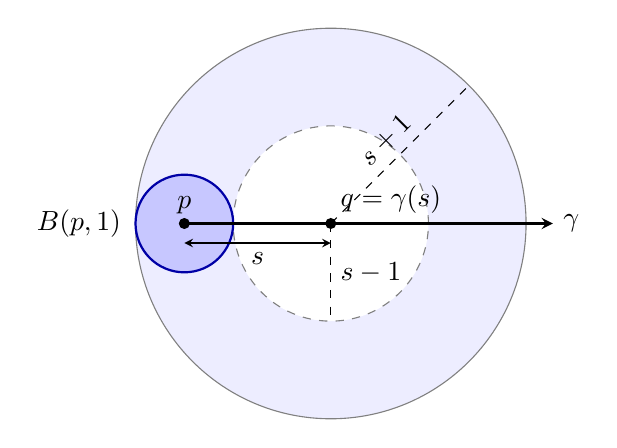
\begin{tikzpicture}[x=.62cm,y=.62cm,>=stealth]
	\fill[blue!7] (0,0) circle (4);
	\fill[white] (0,0) circle (2);
	\draw[gray] (0,0) circle (4);
	\draw[gray,dashed] (0,0) circle (2);
	\filldraw[fill=blue!22,draw=blue!65!black,thick] (-3,0) circle (1);
	\draw[thick,->] (-3,0)--(4.55,0) node[right] {\(\gamma\)};
	\draw[dashed] (0,0)--(2.828,2.828) node[midway,above,sloped] {\(s+1\)};
	\draw[dashed] (0,0)--(0,-2) node[midway,right] {\(s-1\)};
	\draw[<->] (-3,-.4)--(0,-.4) node[midway,below] {\(s\)};
	\fill (-3,0) circle (2pt) node[above] {\(p\)};
	\fill (0,0) circle (2pt) node[above right] {\(q=\gamma(s)\)};
	\node[left] at (-4.1,0) {\(B(p,1)\)};
\end{tikzpicture}

	\caption{把中心移到射线远点 \(q=\gamma(s)\) 后，固定小球落入半径 \(s-1\) 与 \(s+1\) 之间的球壳。图中的圆示意测地球，包含关系由三角不等式保证。}
	\label{g3:fig:ray-annulus}
\end{figure}

\cref{g3:fig:ray-annulus}显示了换球心的作用：小球本身未变，但容纳它的球壳厚度固定为2，相对半径却越来越小。球壳比较因此迫使大球体积随半径增长。下界的常数保留了 \(V_p(1)\)：非负 Ricci 曲率并不为单位球提供一个只依赖维数的正体积下界。例如，将平坦环面的周长缩小，\(\mathbb R\times T^{n-1}\) 的单位球体积也会变小。

\subsection{覆盖空间中的体积计数}
\label{g3:subsec:0803:02}

设 \(\pi:\widetilde M\to M\) 为万有覆盖，赋予 \(\widetilde M\) 拉回度量 \(\widetilde g=\pi^*g\)。由\cref{g3:prop:riemannian-cover-complete}，基流形完备时，覆盖空间也完备。覆盖变换群 \(\Gamma\) 的每个元素都是等距映射，因为 \(\pi\circ h=\pi\) 蕴含 \(h^*\widetilde g=\widetilde g\)。它在每条纤维上自由且传递，因而给定 \(\widetilde p\in\pi^{-1}(p)\) 后，群元素与轨道点 \(h\widetilde p\) 一一对应。

\begin{proposition}\label{g3:prop:covering-orbit-count}
	设 \((M^n,g)\) 为连通、完备、光滑无边界黎曼流形，\(\pi:(\widetilde M,\widetilde g)\to(M,g)\) 为带拉回度量的万有覆盖，\(\Gamma\) 为覆盖变换群。固定 \(\widetilde p\in\widetilde M\)。存在 \(\varepsilon>0\)，使开球族
	\[
		\{B_{\widetilde g}(h\widetilde p,\varepsilon):h\in\Gamma\}
	\]
	两两不交。记 \(v_\varepsilon=\operatorname{Vol}_{\widetilde g}B(\widetilde p,\varepsilon)\)，以及
	\[
		N_{\widetilde p}(R)
		=\#\{h\in\Gamma:
		d_{\widetilde g}(\widetilde p,h\widetilde p)\le R\}.
	\]
	则 \(0<v_\varepsilon<\infty\)，每个 \(N_{\widetilde p}(R)\) 有限，并且
	\begin{equation}\label{g3:eq:covering-volume-packing}
		N_{\widetilde p}(R)v_\varepsilon
		\le\operatorname{Vol}_{\widetilde g}B(\widetilde p,R+\varepsilon)
		\qquad(R\ge0).
	\end{equation}
	若进一步有 \(n\ge2\) 且 \(\operatorname{Ric}_g\ge0\)，则
	\begin{equation}\label{g3:eq:covering-polynomial-orbit}
		N_{\widetilde p}(R)
		\le\frac{\omega_n}{v_\varepsilon}(R+\varepsilon)^n.
	\end{equation}
\end{proposition}
\begin{proof}
	取 \(p=\pi(\widetilde p)\) 的连通均匀覆盖邻域 \(U\)，并令 \(W\) 是 \(\pi^{-1}(U)\) 中含 \(\widetilde p\) 的那一层。对任意 \(h\in\Gamma\)，集合 \(hW\) 也是一层。若 \(hW=W\)，则 \(\pi|_W\) 的单射性与 \(\pi\circ h=\pi\) 给出 \(h|_W=\mathrm{id}\)。覆盖变换由一点的像唯一确定，所以此时 \(h=\mathrm{id}\)。因此不同覆盖变换给出的层 \(hW\) 两两不交。

	距离拓扑等于流形拓扑，可以选 \(\varepsilon>0\)，使 \(B(\widetilde p,\varepsilon)\subset W\)。等距性给出
	\[
		B(h\widetilde p,\varepsilon)
		=hB(\widetilde p,\varepsilon)\subset hW,
	\]
	故这些小球两两不交，体积都等于 \(v_\varepsilon\)。光滑正体积密度保证 \(v_\varepsilon>0\)；覆盖空间完备，其闭有界球紧，故 \(v_\varepsilon<\infty\)。

	当 \(d(\widetilde p,h\widetilde p)\le R\) 时，三角不等式给出
	\[
		B(h\widetilde p,\varepsilon)
		\subset B(\widetilde p,R+\varepsilon).
	\]
	对满足此条件的任意有限个群元素，把相应小球的体积相加，所得结果不超过右侧大球的体积。后者有限而 \(v_\varepsilon>0\)，所以这样的群元素总数必然有限，并得到\eqref{g3:eq:covering-volume-packing}。

	最后，局部等距保持 Ricci 曲率及度量不等式，所以 \(\operatorname{Ric}_{\widetilde g}\ge0\)。在完备的覆盖空间上应用\cref{g3:thm:bishop-gromov}，得
	\[
		\operatorname{Vol}_{\widetilde g}B(\widetilde p,R+\varepsilon)
		\le\omega_n(R+\varepsilon)^n.
	\]
	代回即得\eqref{g3:eq:covering-polynomial-orbit}。
\end{proof}

这里计数的是覆盖空间中的轨道，右端也必须使用覆盖空间的体积。基流形中的大球会把不同提升识别为同一点，其体积通常不能替代\eqref{g3:eq:covering-volume-packing}的右端。平坦乘积的例子将显示，这一区别会改变增长的次数。

\subsection{有限生成子群的增长约束}
\label{g3:subsec:0803:03}

体积估计控制的是几何位移。为了把它用于抽象群，需选定有限个生成元，并记录至多使用多少个生成元能够到达一个元素。

\begin{definition}\label{g3:def:word-growth}
	设 \(G\) 为群，\(S\subset G\) 为有限对称生成集，即 \(S^{-1}=S\) 且 \(S\) 生成 \(G\)。元素 \(h\in G\) 的\term[zichang]{字长}[word length]定义为
	\[
		|h|_S=\min\{m\ge0:h=s_1\cdots s_m,\ s_i\in S\},
	\]
	其中空乘积表示单位元。记
	\[
		\mathcal B_S(m)=\{h\in G:|h|_S\le m\},
		\qquad \beta_S(m)=\#\mathcal B_S(m).
	\]
	若存在 \(C>0\)，使所有整数 \(m\ge0\) 都满足
	\(\beta_S(m)\le C(m+1)^d\)，则称 \(G\) 具有次数至多为 \(d\) 的\term[duoxiangshizengzhang]{多项式增长}[polynomial growth]。
\end{definition}

这一性质不依赖有限生成集的选择。事实上，若 \(T\) 是另一有限对称生成集，取
\[
	A=\max\bigl(\{1\}\cup\{|s|_T:s\in S\}\bigr),
\]
把每个 \(S\) 中的字母换成至多 \(A\) 个 \(T\) 中的字母，便得到
\(\mathcal B_S(m)\subset\mathcal B_T(Am)\)。交换 \(S,T\) 得到反向的线性尺度比较。因此，多项式上界的次数可以保持，常数则随生成集变化。

\begin{theorem}\label{g3:thm:fundamental-subgroup-growth}
	设 \((M^n,g)\) 为连通、完备、光滑无边界黎曼流形，\(n\ge2\)，且 \(\operatorname{Ric}\ge0\)。则 \(\pi_1(M,p)\) 的每个有限生成子群 \(G\)，相对于任意有限对称生成集 \(S\)，都满足
	\[
		\beta_S(m)\le C_S(m+1)^n
		\qquad(m=0,1,2,\ldots),
	\]
	其中 \(C_S\) 可以依赖流形、基点、子群和生成集。
\end{theorem}
\begin{proof}
	利用万有覆盖的覆盖变换群与基本群的同构，将 \(G\) 看成覆盖变换群 \(\Gamma\) 的子群。选定 \(\widetilde p\in\pi^{-1}(p)\)。若 \(G\) 为平凡群，结论由 \(\beta_S(m)=1\) 得到；以下设 \(G\) 非平凡，并在生成集中删去单位元。令
	\[
		L=\max_{s\in S}d_{\widetilde g}(\widetilde p,s\widetilde p)>0.
	\]
	覆盖变换等距，因此任意 \(g,h\in\Gamma\) 满足
	\[
		d(\widetilde p,gh\widetilde p)
		\le d(\widetilde p,g\widetilde p)
		+d(g\widetilde p,gh\widetilde p)
		=d(\widetilde p,g\widetilde p)
		+d(\widetilde p,h\widetilde p).
	\]
	反复应用可知，若 \(|h|_S\le m\)，则
	\(d(\widetilde p,h\widetilde p)\le mL\)。不同群元素作用于 \(\widetilde p\) 得到不同点，所以
	\[
		\beta_S(m)\le N_{\widetilde p}(mL).
	\]
	应用\cref{g3:prop:covering-orbit-count}，得到
	\[
		\beta_S(m)
		\le\frac{\omega_n}{v_\varepsilon}(mL+\varepsilon)^n
		\le\frac{\omega_n(L+\varepsilon)^n}{v_\varepsilon}(m+1)^n.
	\]
	取最后一个系数为 \(C_S\) 即可。
\end{proof}

定理的量词逐个作用于有限生成子群。证明中，有限生成性恰好用于取得生成元位移的有限上界 \(L\)；所得估计本身没有给出整个基本群的一组有限生成元。另一个直接用途是排除增长过快的子群。例如，自由群 \(F_2=\langle a,b\rangle\) 相对于 \(\{a,a^{-1},b,b^{-1}\}\)，长度恰为 \(m\ge1\) 的约化字有 \(4\cdot3^{m-1}\) 个：第一个字母有四种选择，此后每次排除前一字母的逆元，尚有三种选择。因此 \(F_2\) 不可能作为上述基本群的子群。

\subsection{Euclid、双曲及乘积模型}
\label{g3:subsec:0803:04}

模型计算同时检验小尺度和大尺度。光滑 \(n\) 维度量的小球都有 \(n\) 维 Euclid 主项；大球则会反映曲率累积以及紧方向被填满之后的变化。

\begin{example}\label{g3:exm:euclidean-hyperbolic-volume-growth}
	在 Euclid 空间 \(\mathbb R^n\) 中，
	\[
		V_p(R)=\omega_nR^n
	\]
	对所有 \(R>0\) 成立。对曲率为 \(-a^2\) 的双曲模型，取 \(a>0\)、\(n\ge2\)，其全局极坐标度量为
	\[
		g=\mathrm dr^2+
		\left(\frac{\sinh(ar)}a\right)^2g_{S^{n-1}}.
	\]
	这里全局坐标可由双曲面
	\[
		-x_0^2+|x|^2=-a^{-2},\qquad x_0>0
	\]
	上的参数式
	\[
		x_0=a^{-1}\cosh(ar),\qquad
		x=a^{-1}\sinh(ar)u,\qquad u\in S^{n-1},
	\]
	直接得到：将其微分代入 \(-\mathrm dx_0^2+|\mathrm dx|^2\)，径向项为 \(\mathrm dr^2\)，角向项为 \((\sinh(ar)/a)^2g_{S^{n-1}}\)，交叉项为零。每条从中心到半径 \(r\) 的曲线长度至少为 \(r\)，因为离开中心后其速度长度不小于径向速度的绝对值；径向曲线达到此下界。故坐标半径就是中心距离，球体积为
	\begin{equation}\label{g3:eq:hyperbolic-volume-growth}
		V_{-a^2,n}(R)
		=\frac{\sigma_{n-1}}{a^{n-1}}
		\int_0^R\sinh(at)^{n-1}\,\mathrm dt.
	\end{equation}
	当 \(R\downarrow0\) 时，\(\sinh(at)/a=t+O(t^3)\)，所以
	\[
		V_{-a^2,n}(R)=\omega_nR^n\bigl(1+O(R^2)\bigr).
	\]
	当 \(R\to\infty\) 时，
	\[
		\sinh(aR)^{n-1}
		\sim 2^{-(n-1)}e^{(n-1)aR}.
	\]
	将积分与 \(e^{(n-1)aR}\) 的比求极限，或对这个渐近式积分，得到
	\begin{equation}\label{g3:eq:hyperbolic-volume-asymptotic}
		V_{-a^2,n}(R)
		\sim
		\frac{\sigma_{n-1}}{2^{n-1}(n-1)a^n}
		e^{(n-1)aR}.
	\end{equation}
	例如 \(n=2\) 时可直接积分：
	\[
		V_{-a^2,2}(R)=\frac{2\pi}{a^2}\bigl(\cosh(aR)-1\bigr).
	\]
	这里的指数增长说明，非负 Ricci 假设对多项式体积上界具有实质作用。
\end{example}

\begin{example}\label{g3:exm:flat-product-volume-growth}
	设 \(a,b\ge1\) 为整数，\(T^b=\mathbb R^b/\Lambda\) 为平坦环面，赋予
	\[
		M=\mathbb R^a\times T^b
	\]
	乘积度量。其总维数为 \(n=a+b\)，曲率恒为零。记环面直径为 \(D>0\)、体积为 \(v_T>0\)，固定中心 \((0,y_0)\)。

	先核对距离。任意从 \((0,y_0)\) 到 \((x,y)\) 的分片光滑曲线 \((\alpha,\beta)\) 都满足
	\[
		\int\sqrt{|\dot\alpha|^2+|\dot\beta|^2}
		\ge
		\sqrt{\left(\int|\dot\alpha|\right)^2+
		\left(\int|\dot\beta|\right)^2}
		\ge\sqrt{|x|^2+d_T(y_0,y)^2}.
	\]
	第一个不等式是对向量值函数
	\((|\dot\alpha|,|\dot\beta|)\) 的积分三角不等式。反过来，分别取两个因子中的最短线，并将它们参数化在 \([0,1]\) 上，使速度长度恒为各自端点距离，便达到下界。因此
	\[
		d_M((0,y_0),(x,y))^2=|x|^2+d_T(y_0,y)^2.
	\]
	两个因子均完备，距离公式又说明乘积中的 Cauchy 序列逐分量收敛，所以 \(M\) 完备。

	用乘积体积密度逐纤维积分，可得对所有 \(R>0\) 都成立的精确公式
	\begin{equation}\label{g3:eq:flat-product-volume-formula}
		V_{(0,y_0)}(R)
		=\omega_a\int_{T^b}
		\bigl(R^2-d_T(y_0,y)^2\bigr)_+^{a/2}\,\mu_T(y),
	\end{equation}
	其中 \(s_+=\max\{s,0\}\)。因为 \(0\le d_T(y_0,y)\le D\)，当 \(R>D\) 时，
	\begin{equation}\label{g3:eq:flat-product-volume-bounds}
		\omega_av_T(R^2-D^2)^{a/2}
		\le V_{(0,y_0)}(R)
		\le\omega_av_TR^a.
	\end{equation}
	特别地，对 \(R\ge2D\)，有
	\[
		\left(\frac34\right)^{a/2}\omega_av_TR^a
		\le V_{(0,y_0)}(R)
		\le\omega_av_TR^a,
	\]
	而令 \(R\to\infty\) 得到
	\[
		V_{(0,y_0)}(R)\sim\omega_av_TR^a.
	\]

	小尺度却仍是 \(n=a+b\) 维的。设
	\(\rho=\frac12\min_{\lambda\in\Lambda\setminus\{0\}}|\lambda|>0\)。
	当 \(0<R<\rho\) 时，覆盖映射
	\(\mathbb R^{a+b}\to\mathbb R^a\times T^b\)
	在 Euclid 半径 \(R\) 的球上限制为到上述球的微分同胚，并保持黎曼度量：任意 \(y\) 的最短代表可由使 \(|\widetilde y+\lambda|\) 最小的格点给出，距离公式保证满射；两个球内点若相差非零格向量，其距离小于 \(2R<2\rho\)，又与格向量长度下界矛盾。因此
	\[
		V_{(0,y_0)}(R)=\omega_{a+b}R^{a+b}
		\qquad(0<R<\rho).
	\]
	公式\eqref{g3:eq:flat-product-volume-formula}描述了从小尺度到大尺度的整个过渡。当 \(a=1\) 时，大球体积恰为线性量级，说明\cref{g3:thm:noncompact-volume-growth}的线性下界在一般情形下不能提高到更大的幂次。
\end{example}

上述乘积的万有覆盖是 \(\mathbb R^{a+b}\)，覆盖变换沿环面因子的格点作平移。因此，基流形的大球按 \(R^a\) 增长，覆盖空间的大球却按 \(R^{a+b}\) 增长。覆盖体积计数使用后一个增长率，正是因为它需要把所有不同提升的小球分别容纳进去。
% 纲要条目排为编号小节标题，并进入目录与书签；说明段仍保留于纲要注释中。

% !TeX root = ../../Book3.tex
% 纲要标题：### 8.4 曲率比较的适用范围
% 纲要位置：几何学计划纲要.md，第 2418 行。
% 正文状态：初稿；尚未正式审核。

% 纲要内容开始
% 
% * 非负 Ricci 与非负截面曲率的区别
% * 塌缩时体积信息的变化
% * Busemann 函数与分裂定理
% 
% ---
% 
% 纲要内容结束

\section{曲率比较的适用范围}
\label{g3:sec:0804}

本章的比较把曲率信息逐步变成长度、体积与群的计数。取迹和积分使这些结论适用范围很广，也会丢失某些方向与尺度的信息。本节用具体模型辨别这些损失，再考察从距离比较走向整体乘积分解还需要哪些工具。

\subsection{非负 Ricci 与非负截面曲率的区别}
\label{g3:subsec:0804:01}

若 \(T,e_1,\ldots,e_{n-1}\) 是一点处的正交单位基，则
\[
	\operatorname{Ric}(T,T)=\sum_{i=1}^{n-1}K(T\wedge e_i).
\]
因此 \(K\ge k\) 推出 \(\operatorname{Ric}\ge(n-1)kg\)。二维只有一个截面，\(\operatorname{Ric}=Kg\)，这两个条件等价；从三维起，一个方向的负截面曲率可以被其他方向的正曲率补偿。

例如\cref{g3:exm:ricci-positive-sectional-negative}给出的三维代数曲率张量满足
\[
	K(e_1\wedge e_2)=-1,\qquad
	K(e_1\wedge e_3)=K(e_2\wedge e_3)=2,
	\qquad \operatorname{Ric}=\operatorname{diag}(1,1,4).
\]
\Cref{g3:prop:curvature-local-realization}把它实现为一点附近的光滑度量，严格正的 Ricci 与指定的负截面在足够小的邻域中同时保留。这说明即使在局部，正 Ricci 也不能替代逐截面的正性；该构造本身没有给出全局的 Ricci 下界。第七章的迹比较正好体现这个区别：它控制径向形算子的迹，而不能分别控制其全部特征值。只有达到模型等号时，平方和估计的等号才进一步迫使各个特征值相等。

另一种容易混淆的条件是“处处严格为正”和“有统一的正常数下界”。后者是本章直径定理真正使用的条件。

\begin{example}\label{g3:exm:positive-paraboloid}
	考虑 Euclid 空间中的抛物面
	\[
		P=\{(x,y,z)\in\mathbb R^3:z=x^2+y^2\},
	\]
	赋予诱导度量。用水平极坐标 \((\rho,\theta)\) 表示，得到
	\[
		g=(1+4\rho^2)\,\mathrm d\rho^2+\rho^2\,\mathrm d\theta^2.
	\]
	在全局图坐标 \((x,y)\) 中，\(g=\mathrm dx^2+\mathrm dy^2+4(x\,\mathrm dx+y\,\mathrm dy)^2\ge g_{\mathrm E}\)。所以任一 \(g\)-Cauchy 序列在 Euclid 坐标中收敛；在极限点的紧坐标邻域中，\(g\le Cg_{\mathrm E}\)，它也按 \(g\) 收敛。这证明 \(P\) 完备。全局图坐标又表明它非紧。

	令 \(s(\rho)=\int_0^\rho\sqrt{1+4u^2}\,\mathrm du\)，把度量写成 \(\mathrm ds^2+f(s)^2\mathrm d\theta^2\)，其中 \(f(s)=\rho\)。于是
	\[
		f'(s)=\frac1{\sqrt{1+4\rho^2}},\qquad
		f''(s)=-\frac{4\rho}{(1+4\rho^2)^2}.
	\]
	由\cref{g3:prop:warped-product-curvature}，在 \(\rho>0\) 处
	\[
		K=-\frac{f''}{f}=\frac4{(1+4\rho^2)^2}>0.
	\]
	在顶点处由光滑性取极限仍得 \(K=4\)。因此 \(\operatorname{Ric}=Kg\) 处处正定，但 \(K\to0\) 于无穷远，不能选取本章直径定理所需的统一 \(k>0\)。
\end{example}

这个例子也把两个尺度联系起来：每一点附近都有正曲率的局部几何，远处越来越小的曲率却容许测地线无限延伸。章末将直接计算其球面积，得到介于线性与二次之间的增长。

\subsection{塌缩时体积信息的变化}
\label{g3:subsec:0804:02}

体积比较给出上界以及不同半径之间的比值控制。它是否同时给出某个固定半径球的一致正体积下界？以下平坦例子说明，还必须指定一个不退化的体积尺度。

\begin{example}\label{g3:exm:collapsing-flat-tori}
	设 \(n\ge2\)、\(0<\varepsilon\le1\)，取平坦乘积
	\[
		T_\varepsilon=(\mathbb R/\mathbb Z)^{n-1}
		\times(\mathbb R/\varepsilon\mathbb Z).
	\]
	它的曲率恒为零，基本区域的体积为 \(\varepsilon\)。乘积距离由各个圆周的最短弧长平方求和得到，故
	\[
		\operatorname{diam}T_\varepsilon
		=\frac12\sqrt{n-1+\varepsilon^2},\qquad
		\operatorname{inj}(T_\varepsilon)=\frac\varepsilon2.
	\]
	最后一式也可从格商看出：长度最短的非零格向量为 \(\varepsilon\)，指数映射在半径小于其一半时单射，在一半处遇到相反的最短弧。

	固定一点 \(p\)，仍以 \(\omega_j\) 表示 Euclid 单位 \(j\) 维球体积。若 \(r<\varepsilon/2\)，则 \(B(p,r)\) 是 Euclid 球，体积恰为 \(\omega_n r^n\)。若 \(\varepsilon/2<r<1/2\)，短圆周上的所有点距离基点都不超过 \(\varepsilon/2\)，于是
	\begin{equation}\label{g3:eq:collapsed-ball-estimate}
		\varepsilon\omega_{n-1}(r^2-\varepsilon^2/4)^{(n-1)/2}
		\le\operatorname{Vol}_g B(p,r)
		\le\varepsilon\omega_{n-1}r^{n-1}.
	\end{equation}
	确切地说，球内含半径 \(\sqrt{r^2-\varepsilon^2/4}\) 的底空间球与整条短圆周的乘积，并包含于半径 \(r\) 的底空间球与短圆周的乘积；在 \(r<1/2\) 时这些底空间球均为 Euclid 球。这就证明了两侧体积估计。

	固定 \(0<r<1/2\) 并令 \(\varepsilon\downarrow0\)，有
	\[
		\operatorname{Vol}_g B(p,r)\longrightarrow0,
		\qquad
		\frac{\operatorname{Vol}_g B(p,r)}\varepsilon
		\longrightarrow\omega_{n-1}r^{n-1}.
	\]
	投影 \(\pi:T_\varepsilon\to(\mathbb R/\mathbb Z)^{n-1}\) 还满足
	\[
		d(\pi x,\pi y)\le d(x,y)
		\le\sqrt{d(\pi x,\pi y)^2+\varepsilon^2/4}
		\le d(\pi x,\pi y)+\varepsilon/2.
	\]
	因此短圆周方向在固定尺度的距离测量中逐渐消失；体积趋零和距离趋近低一维空间发生在同一模型中。
\end{example}

这种有些方向的长度尺度趋零、相应体积退化的现象称为\term[tasuo]{塌缩}[collapse]。在上例中，先固定 \(\varepsilon\) 再令 \(r\downarrow0\)，总能看到 \(n\) 维 Euclid 体积；先固定 \(r\) 再令 \(\varepsilon\downarrow0\)，却会失去一个方向。小球的局部维数与一族度量在固定尺度下的退化因而是不同问题。

给定尺度上的一致正体积下界通常称为该尺度的\term[fei tansuo]{非塌缩}[noncollapse]条件。体积比较能够把已有的这种下界传到邻近中心及更小半径。

\begin{proposition}\label{g3:prop:noncollapse-propagation}
	记 \(V_p(r)=\operatorname{Vol}_g B(p,r)\)，\(\sigma_{n-1}\) 为 Euclid 单位球面的面积，\(V_{k,n}(r)=\sigma_{n-1}\int_0^r s_k(t)^{n-1}\,\mathrm dt\) 为常曲率模型球体积。
	取 \(k\in\mathbb R\)。记 \(s_k\) 为 \(s_k''+ks_k=0\)、\(s_k(0)=0\)、\(s_k'(0)=1\) 的解，\(b_k=\pi/\sqrt k\) 当 \(k>0\)，否则 \(b_k=\infty\)。
	设 \((M^n,g)\) 连通、完备、光滑且无边界，\(n\ge2\)，\(\operatorname{Ric}\ge(n-1)kg\)。设 \(p,q\in M\)、\(d(p,q)\le D\)，且 \(r_0>0\)、\(\operatorname{Vol}_g B(p,r_0)\ge v_0>0\)。若 \(0<r\le D+r_0<b_k\)，则
	\[
		\operatorname{Vol}_g B(q,r)
		\ge\frac{V_{k,n}(r)}{V_{k,n}(D+r_0)}v_0.
	\]
\end{proposition}
\begin{proof}
	三角不等式给出 \(B(p,r_0)\subset B(q,D+r_0)\)。把\cref{g3:thm:bishop-gromov}用于中心 \(q\) 以及半径 \(r,D+r_0\)，得
	\[
		\frac{\operatorname{Vol}_g B(q,r)}{V_{k,n}(r)}
		\ge\frac{\operatorname{Vol}_g B(q,D+r_0)}{V_{k,n}(D+r_0)}
		\ge\frac{v_0}{V_{k,n}(D+r_0)}.
	\]
\end{proof}

特别地，当 \(\operatorname{Ric}\ge0\) 时，下界变成 \(v_0(r/(D+r_0))^n\)，且没有有限的模型半径限制。这里体积的绝对尺度来自假设中的 \(v_0\)；曲率比较负责传播它。平坦环面族中这个初始体积本身趋零，所以与该命题完全相容。

\subsection{Busemann 函数与分裂定理}
\label{g3:subsec:0804:03}

在 Euclid 空间中，一条定向直线给出一个线性坐标；与它垂直的超平面组成一个乘积分解。在一般完备流形中，可以先把测地射线上的点推向无穷远，再从距离中减去趋于无穷的常数，尝试得到相应坐标。

\begin{definition}\label{g3:def:busemann-function}
	设 \((M,g)\) 是连通、完备、光滑无边界黎曼流形，\(\gamma:[0,\infty)\to M\) 为单位速测地射线，即 \(d(\gamma(s),\gamma(t))=|s-t|\)。函数
	\begin{equation}\label{g3:eq:busemann-sign}
		b_\gamma(x)=\lim_{t\to\infty}\bigl(t-d(x,\gamma(t))\bigr)
	\end{equation}
	称为 \(\gamma\) 的\term[Busemann hanshu]{Busemann 函数}[Busemann function]。\footnote{Herbert Busemann（1905--1994），德国出生的美国数学家，研究度量几何、凸性与测地线。}本书采用沿射线增加的符号，因而下面将有 \(b_\gamma(\gamma(s))=s\)。
\end{definition}

\symidx{\(b_\gamma\)：沿射线增加的 Busemann 函数}
定义中的极限并不要求曲率条件，其存在性来自三角不等式。完备非紧流形上已有\cref{g3:lem:complete-noncompact-ray}保证这样的射线存在。

\begin{proposition}\label{g3:prop:busemann-basic}
	设 \((M,g)\) 连通、完备、光滑且无边界，\(\gamma:[0,\infty)\to M\) 为单位速测地射线。则式\eqref{g3:eq:busemann-sign}的极限处处存在，且在每个紧集上一致收敛。函数 \(b_\gamma\) 为1-Lipschitz，满足
	\[
		|b_\gamma(x)|\le d(x,\gamma(0)),\qquad
		b_\gamma(\gamma(s))=s\quad(s\ge0).
	\]
\end{proposition}
\begin{proof}
	记 \(b_t(x)=t-d(x,\gamma(t))\)。对 \(t\ge s\)，由射线的最短性及三角不等式，
	\[
		d(x,\gamma(t))\le d(x,\gamma(s))+t-s,
		\qquad b_t(x)\ge b_s(x).
	\]
	又由三角不等式的两种写法，\(-d(x,\gamma(0))\le b_t(x)\le d(x,\gamma(0))\)。所以 \(b_t(x)\) 单调有界，极限存在。每个 \(b_t\) 都为1-Lipschitz，取极限保留这一性质及上述界。在射线上，对 \(t\ge s\) 直接计算 \(b_t(\gamma(s))=t-(t-s)=s\)。

	最后设 \(K\subset M\) 紧。任给 \(\eta>0\)，取有限个半径 \(\eta\) 的球覆盖 \(K\)，球心取在 \(K\) 中。在这有限个球心上，当 \(t\) 足够大时均有 \(|b_t-b_\gamma|<\eta\)。对任一 \(x\in K\)，选取相距小于 \(\eta\) 的球心；使用 \(b_t,b_\gamma\) 的1-Lipschitz 性，得到 \(|b_t(x)-b_\gamma(x)|<3\eta\)。这证明紧集上的一致收敛。
\end{proof}

在 \(\mathbb R^n\) 中取 \(\gamma(t)=tv\)、\(|v|=1\)。有理化给出
\[
	 t-|x-tv|
	=\frac{2t\langle x,v\rangle-|x|^2}{t+|x-tv|}
	\longrightarrow\langle x,v\rangle.
\]
因此这一极限确实恢复沿 \(v\) 的线性坐标。一般流形上的 \(b_\gamma\) 首先只有 Lipschitz 正则性；距离函数的割迹也不能在取极限时直接忽略。第七章的分布比较正好适用于这一过程。

\begin{proposition}\label{g3:prop:busemann-weak-laplacian}
	设 \((M^n,g)\) 连通、完备、光滑且无边界，\(n\ge2\)，\(\operatorname{Ric}\ge0\)，\(\gamma\) 为单位速测地射线。以 \(\Delta=-\operatorname{div}\nabla\) 记本书的 Laplace 算子，则
	\[
		\Delta b_\gamma\le0
	\]
	在分布意义下成立，即对每个非负 \(\phi\in C_c^\infty(M)\)，\(\int_M b_\gamma\Delta\phi\,\mu_g\le0\)。
\end{proposition}
\begin{proof}
	令 \(K=\operatorname{supp}\phi\)，取 \(C\) 使 \(d(x,\gamma(0))\le C\) 对 \(x\in K\) 成立。若 \(t>C\)，则 \(r_t(x)=d(x,\gamma(t))\ge t-C>0\) 于 \(K\)。由\cref{g3:thm:distributional-laplacian-comparison}在 \(k=0\) 时的结论，\(\Delta r_t\ge-(n-1)/r_t\)。又因紧支测试函数满足 \(\int_M\Delta\phi\,\mu_g=0\)，有
	\[
		\int_M b_t\Delta\phi\,\mu_g
		=-\int_M r_t\Delta\phi\,\mu_g
		\le\int_M\frac{n-1}{r_t}\phi\,\mu_g
		\le\frac{n-1}{t-C}\int_M\phi\,\mu_g.
	\]
	在 \(K\) 上 \(b_t\) 一致趋于 \(b_\gamma\)，令 \(t\to\infty\)，右端趋于零，即得所需分布不等式。
\end{proof}

设现在有一条\term[cedi zhixian]{测地直线}[geodesic line] \(\gamma:\mathbb R\to M\)，即单位速测地线且任意有限段都最短，等价地 \(d(\gamma(s),\gamma(t))=|s-t|\)。对它的两个方向分别构造
\[
	 b_+(x)=\lim_{t\to\infty}\bigl(t-d(x,\gamma(t))\bigr),\qquad
	 b_-(x)=\lim_{t\to\infty}\bigl(t-d(x,\gamma(-t))\bigr).
\]
三角不等式给出 \(d(x,\gamma(t))+d(x,\gamma(-t))\ge2t\)，所以
\begin{equation}\label{g3:eq:two-busemann-functions}
	 b_++b_-\le0,\qquad
	 b_+(\gamma(s))+b_-(\gamma(s))=s-s=0.
\end{equation}
若 \(\operatorname{Ric}\ge0\)，两者又满足 \(\Delta b_\pm\le0\)。于是 \(b_++b_-\) 是一个在直线上达到全局最大值的弱次调和函数；这里“次调和”对应 \(\operatorname{div}\nabla\ge0\)，也就是本书的 \(\Delta\le0\)。

要把这一事实变成乘积分解，还需三步分析。首先，用适用于上述弱不等式的强最大值原理推出 \(b_++b_-=0\)，从而两者弱调和；其次，用椭圆正则性取得光滑性，并借从任意点出发的渐近射线证明 \(|\nabla b_+|=1\)；最后用 Bochner 公式推出 \(\operatorname{Hess}b_+=0\)。这时 \(\nabla b_+\) 才成为平行单位场，其流把等值面与实直线组成整体等距乘积。

这些步骤及所需的弱最大值、正则性工具将在\secref{g3:sec:1505}汇合，证明如下结论：若 \((M^n,g)\) 连通、完备、光滑、无边界且 \(\operatorname{Ric}\ge0\)，并含有一条测地直线，则 \(M\) 等距于 \(\mathbb R\times N\)，其中 \(N\) 是完备的 \((n-1)\) 维黎曼流形。这里要求的是双向都保持最短的直线；单有从一点出发的射线，只保证 Busemann 函数存在，尚不能使式\eqref{g3:eq:two-busemann-functions}的两侧构造成立。
% 纲要条目排为编号小节标题，并进入目录与书签；说明段仍保留于纲要注释中。


\begin{chaptersummary}
	固定端点的正弦试探场把 Ricci 的统一正下界变成最短线长度的上界。完备性提供最短线并把有界性提升为紧性；把相同论证用于拉回度量下的万有覆盖，再以紧离散纤维计数，就得到基本群有限性。

	\ProseParagraphBreak

	径向密度除以模型密度后不增，在割时的向下跳跃保留了这一方向。沿球面与半径积分，便得到球体积比及球壳的相对比较；最大体积的等号同时排除球内割点和径向伸缩中的亏损，因而恢复模型球的度量。将球心移向射线远处给出非紧流形的线性体积下界，在覆盖中放入两两不交的小球则把体积上界变成轨道与群的增长上界。

	\ProseParagraphBreak

	Ricci 条件控制方向和，塌缩模型说明它也不能单独固定一个正体积尺度。射线的 Busemann 函数把距离比较传到无穷远，但其最初的正则性只有 Lipschitz；由弱 Laplace 不等式取得光滑平行梯度，需要后续的最大值原理、椭圆正则性与 Bochner 公式。下一章将回到截面曲率，研究全局指数映射、空间形式与测地三角比较；度量收敛与塌缩的系统语言在第十章建立。
\end{chaptersummary}

\BookExercises

\begin{exercise}\label{g3:ex:myers-unbounded-finite-group-order}
	在单位球面
	\[
		S^3=\{(z_1,z_2)\in\mathbb C^2:|z_1|^2+|z_2|^2=1\}
	\]
	上取圆度量。对整数 \(m\ge2\)，令 \(\zeta=e^{2\pi\mathrm{i}/m}\)，以
	\[
		A(z_1,z_2)=(\zeta z_1,\zeta z_2)
	\]
	生成循环群 \(\Gamma_m\)。证明商 \(M_m=S^3/\Gamma_m\) 是紧连通无边界光滑三维流形，具有截面曲率恒为 \(1\) 的商度量，并且
	\[
		\operatorname{Ric}_{M_m}=2g_m,\qquad
		\operatorname{diam}(M_m)\le\pi,\qquad
		\pi_1(M_m)\cong\mathbb Z/m\mathbb Z.
	\]
	据此说明，固定维数、正 Ricci 下界和直径上界，仍不能由 Bonnet--Myers 定理得到基本群阶的统一上界。
\end{exercise}
\begin{solution}
	\(A\) 是 \(\mathbb R^4\) 上的正交变换，因此保持球面及圆度量。若 \(A^jz=z\)，至少有一个 \(z_i\ne0\)，故 \(\zeta^j=1\)，即 \(m\mid j\)。所以群作用自由，且每条轨道恰有 \(m\) 个点。

	在每个 \(z\in S^3\) 处，选小球 \(U\)，使 \(U,A(U),\ldots,A^{m-1}(U)\) 两两不交；有限轨道中不同点的正距离保证可以这样取。商投影限制到 \(U\) 为同胚，利用这些限制把球面坐标送到商上，过渡映射是原坐标变换与某个 \(A^j\) 的复合，因而光滑。不同有限轨道可取互不相交的饱和邻域，故商 Hausdorff；商映射开，球面的可数基之像给出商的可数基。因此商确为光滑三维无边界流形，投影为 \(m\) 叶光滑覆盖。商还是紧连通空间，因为它是紧连通球面的连续像。

	各 \(A^j\) 为等距变换，故局部搬运的度量在覆盖片之间一致，给出使投影局部等距的商度量。局部等距保持曲率，所以 \(K_{M_m}=1\)、\(\operatorname{Ric}_{M_m}=2g_m\)。紧性给出完备性，\cref{g3:thm:bonnet-myers}在 \(n=3,k=1\) 时得到直径界 \(\pi\)。

	第一卷第5章第2节“高维球面的单连通性”命题给出 \(S^3\) 单连通，故此覆盖就是万有覆盖。其覆盖变换群恰为 \(\Gamma_m\)：已给变换在一个纤维上传递，而任意覆盖变换由一点的像唯一确定，不可能还有其他变换。第一卷第5章第4节的万有覆盖变换群结论于是给出 \(\pi_1(M_m)\cong\Gamma_m\cong\mathbb Z/m\mathbb Z\)。当 \(m\to\infty\) 时，维数和上述曲率、直径常数均不变，群阶却无界。
\end{solution}

\begin{exercise}\label{g3:ex:myers-positive-outside-ball}
	设 \((M,g)\) 是连通、完备、无边界的 \(n\ge2\) 维光滑黎曼流形。假设存在 \(p\in M\)、\(R\ge0\)、\(k>0\)，使所有满足 \(d(p,x)\ge R\) 的点处都有
	\[
		\operatorname{Ric}_x\ge(n-1)k g_x.
	\]
	球 \(B(p,R)\) 内不作曲率符号假设。证明
	\[
		M=\overline B\left(p,R+\frac\pi{\sqrt k}\right),
	\]
	从而 \(M\) 紧，且 \(\operatorname{diam}(M)\le2R+2\pi/\sqrt k\)。解释为什么不能把基本群有限性的结论也直接照搬到这个条件下。
\end{exercise}
\begin{solution}
	任取 \(q\in M\)，令 \(\ell=d(p,q)\)。若 \(\ell\le R\)，所求距离界已成立。若 \(\ell>R\)，Hopf--Rinow 定理给出单位速最短测地线 \(\gamma:[0,\ell]\to M\)，从 \(p\) 连到 \(q\)。它的每个子段都最短，且 \(d(p,\gamma(t))=t\)；否则用更短曲线替换起始段就会缩短整条曲线。因此 \(\gamma|_{[R,\ell]}\) 全部位于满足 Ricci 下界的区域。将此段的起始参数平移到零，\cref{g3:lem:myers-index-test}给出
	\[
		\ell-R\le\frac\pi{\sqrt k}.
	\]
	这说明全部点都位于所列闭球中。该球由完备性和 Hopf--Rinow 定理为紧集，所以 \(M\) 紧；任意两点之间经 \(p\) 使用三角不等式，得到直径界。

	但这里的曲率条件允许整个流形都落在 \(B(p,R)\) 中，此时球外条件为空。例如任取紧平坦环面，选 \(R\) 大于它的直径，就对任何 \(k>0\) 满足题设，而其万有覆盖为 \(\mathbb R^n\)、覆盖变换群为 \(\mathbb Z^n\)，所以基本群无限。覆盖上也不能把坏区域的原像视为一个有界球；它可以包含无限多张彼此远离的覆盖片。因此这道题只推出基空间紧性，不能提供覆盖上的同样直径界。
\end{solution}

\begin{exercise}\label{g3:ex:myers-product-diameter}
	设 \(m,q\ge2\)、\(n=m+q\)，在 \(M=S^m(a)\times S^q(b)\) 上取乘积度量。
	\begin{enumerate}
		\item 求使 \(\operatorname{Ric}_M\ge(n-1)k g\) 成立的最大常数 \(k\)。
		\item 证明乘积中的距离平方是两个因子距离平方之和，进而求 \(\operatorname{diam}(M)\)。
		\item 取
		\[
			a^2=\frac{m-1}{n-1},\qquad b^2=\frac{q-1}{n-1}.
		\]
		计算 Ricci 曲率和直径，比较 Bonnet--Myers 给出的界，并指出一个截面曲率为零的平面。
	\end{enumerate}
\end{exercise}
\begin{solution}
	由球面的 Ricci 公式及\cref{g3:prop:product-curvature}，
	\[
		\operatorname{Ric}_M
		=\frac{m-1}{a^2}g_1\oplus\frac{q-1}{b^2}g_2.
	\]
	把向量分别限制到两个因子，得到必要条件；再对一般向量的正交分量相加，得到充分性。因此最大常数为
	\[
		k_{\max}=\frac1{n-1}
		\min\left\{\frac{m-1}{a^2},\frac{q-1}{b^2}\right\}>0.
	\]

	对连接两点的任意乘积曲线 \(c=(c_1,c_2)\)，令两个因子的长度分别为 \(L_1,L_2\)。对速度向量应用平面中的 Cauchy--Schwarz 不等式并积分，得到
	\[
		\operatorname{Len}(c)
		=\int\sqrt{|\dot c_1|^2+|\dot c_2|^2}\,\mathrm{d}t
		\ge\sqrt{L_1^2+L_2^2}\ge\sqrt{d_1^2+d_2^2}.
	\]
	具体地，第一步在 \(L_1^2+L_2^2>0\) 时将单位向量 \((L_1,L_2)/\sqrt{L_1^2+L_2^2}\) 与 \((|\dot c_1|,|\dot c_2|)\) 配对后积分即可；零长度情形直接成立。反向估计由两个因子的最短测地线给出：把它们都在 \([0,1]\) 上常速参数化，速度长度分别为 \(d_1,d_2\)，乘积曲线的长度正是 \(\sqrt{d_1^2+d_2^2}\)。因此
	\[
		d_M((x_1,x_2),(y_1,y_2))^2
		=d_1(x_1,y_1)^2+d_2(x_2,y_2)^2.
	\]
	球面的直径分别为 \(\pi a,\pi b\)，同时选两对对径点便达到最大值，所以
	\[
		\operatorname{diam}(M)=\pi\sqrt{a^2+b^2}.
	\]

	在题设的归一化下，两个 Ricci 系数都为 \(n-1\)，故 \(\operatorname{Ric}_M=(n-1)g\)，\(k_{\max}=1\)。实际直径为
	\[
		\pi\sqrt{\frac{n-2}{n-1}}<\pi,
	\]
	严格小于 Bonnet--Myers 的模型上界。分别从两个因子选非零向量，它们张成的混合截面曲率为零。因此 Ricci 下界恰取归一化值，并不要求每个截面都有同样的正下界，也不迫使直径达到模型值。
\end{solution}

\begin{exercise}\label{g3:ex:flat-cylinder-ball-volume}
	在平坦圆柱 \(M=(\mathbb R/\ell\mathbb Z)\times\mathbb R\) 上取乘积度量，其中 \(\ell>0\)。固定 \(p=([0],0)\)，记 \(d=\ell/2\)、\(V(r)=\operatorname{Vol}(B(p,r))\)。
	\begin{enumerate}
		\item 用初始单位向量 \(u=(u_1,u_2)\) 表示割时 \(c_p(u)\)，并求割时以前的径向密度。
		\item 证明
		\[
			V(r)=
			\begin{cases}
				\pi r^2,&0<r\le d,\\
				2d\sqrt{r^2-d^2}+2r^2\arcsin(d/r),&r>d.
			\end{cases}
		\]
		\item 证明 \(V(r)/(\pi r^2)\) 在 \((d,\infty)\) 上严格递减，并求 \(V(r)/r\) 在无穷远的极限。解释局部平坦为何不保证所有半径上的模型体积等号。
	\end{enumerate}
\end{exercise}
\begin{solution}
	覆盖映射 \(\mathbb R^2\to M\) 是局部等距；连接 \(p\) 与 \(([x],y)\) 的曲线提升后，其终点为某个 \((x+j\ell,y)\)。Euclid 线段给出这些提升中各自的最短长度，因此
	\[
		d_M(p,([x],y))=\min_{j\in\mathbb Z}\sqrt{(x+j\ell)^2+y^2}.
	\]
	选择 \(-d\le x\le d\) 的代表元，最小值为 \(\sqrt{x^2+y^2}\)；当 \(|x|<d\) 时最短提升唯一，在 \(|x|=d\) 时有两条。因此
	\[
		c_p(u)=
		\begin{cases}d/|u_1|,&u_1\ne0,\\ \infty,&u_1=0.\end{cases}
	\]
	曲率为零，法向 Jacobi 方程是 \(A''=0\)，初值给出 \(A(t)=t\)。故割时以前 \(\theta_p(t,u)=t\)，而截断密度比为
	\[
		\frac{\overline\theta_p(t,u)}t=\mathbf1_{\{t<c_p(u)\}}.
	\]

	取基本条带 \([-d,d]\times\mathbb R\)。其两条边识别，但边的二维体积为零，所以球体积等于 Euclid 圆盘 \(x^2+y^2<r^2\) 与这个条带的交的面积。当 \(r\le d\) 时得到整个圆盘。当 \(r>d\) 时，
	\[
		V(r)=\int_{-d}^d2\sqrt{r^2-x^2}\,\mathrm dx
		=2d\sqrt{r^2-d^2}+2r^2\arcsin(d/r),
	\]
	其中使用原函数
	\(\frac12(x\sqrt{r^2-x^2}+r^2\arcsin(x/r))\)。两个表达式在 \(r=d\) 处都等于 \(\pi d^2\)。

	对 \(r>d\) 求导，含 \(1/\sqrt{r^2-d^2}\) 的两项相消，留下
	\[
		V'(r)=4r\arcsin(d/r),\qquad
		\frac{\mathrm d}{\mathrm dr}\frac{V(r)}{\pi r^2}
		=-\frac{4d\sqrt{r^2-d^2}}{\pi r^3}<0.
	\]
	再由 \(\sqrt{r^2-d^2}/r\to1\) 及 \(r\arcsin(d/r)\to d\)，得到
	\[
		\lim_{r\to\infty}\frac{V(r)}r=4d=2\ell.
	\]
	每条射线的未截断密度都与平面相同；超过 \(d\) 后，一批方向已到割点，截断使实际贡献变为零。这一正测度方向上的损失使体积比严格下降。
\end{solution}

\begin{exercise}\label{g3:ex:volume-comparison-packing}
	设 \((M^n,g)\) 连通、完备、光滑且无边界，\(n\ge2\)、\(\operatorname{Ric}\ge0\)。固定 \(p\in M\)、\(R>0\) 及 \(0<r\le R\)。设 \(x_i\in B(p,R)\)，且开球 \(B(x_i,r)\) 两两不交。证明这样的球只有有限个，其个数 \(N\) 满足
	\[
		N\le\left(\frac{2(R+r)}r\right)^n
		\le\left(\frac{4R}r\right)^n.
	\]
	证明时不对各个小球的体积另加统一正下界假设。
\end{exercise}
\begin{solution}
	对每个中心 \(x_i\)，三角不等式给出
	\[
		B(p,R)\subset B(x_i,2R),\qquad
		B(x_i,r)\subset B(p,R+r).
	\]
	由于 \(r\le R<2R\)，以 \(x_i\) 为中心的 Bishop--Gromov 比较给出
	\[
		\operatorname{Vol}(B(x_i,r))
		\ge\left(\frac r{2R}\right)^n\operatorname{Vol}(B(x_i,2R))
		\ge\left(\frac r{2R}\right)^n\operatorname{Vol}(B(p,R)).
	\]
	这正是从大球体积推出的相对下界，并未预设绝对的非塌缩常数。

	先取任意有限子族，设其含 \(N_0\) 个球。由两两不交及包含关系，
	\[
		N_0\left(\frac r{2R}\right)^n\operatorname{Vol}(B(p,R))
		\le\operatorname{Vol}(B(p,R+r))
		\le\left(\frac{R+r}R\right)^n\operatorname{Vol}(B(p,R)).
	\]
	最后一个不等式再次使用体积比比较。正且有限的 \(\operatorname{Vol}(B(p,R))\) 可约去，于是
	\(N_0\le[2(R+r)/r]^n\)。若原球族无限，就能取出任意大的有限子族，矛盾。因此原球族有限，并满足同一个上界。最后利用 \(r\le R\) 得到所写的第二个估计。
\end{solution}

\begin{exercise}\label{g3:ex:euclidean-asymptotic-volume-rigidity}
	设 \((M^n,g)\) 连通、完备、光滑且无边界，\(n\ge2\)、\(\operatorname{Ric}\ge0\)。若存在 \(p\in M\) 使
	\[
		\lim_{r\to\infty}\frac{\operatorname{Vol}(B(p,r))}{\omega_n r^n}=1,
	\]
	证明 \((M,g)\) 与 \(\mathbb R^n\) 全局等距。须说明由不同半径的球上得到的等距如何相容，而不只分别断言每个有限半径的球是 Euclid 球。
\end{exercise}
\begin{solution}
	令 \(Q(r)=\operatorname{Vol}(B(p,r))/(\omega_n r^n)\)。由\cref{g3:thm:bishop-gromov}，\(Q\) 不增且 \(Q(r)\le1\)。另一方面，对任意 \(R>r\)，有 \(Q(r)\ge Q(R)\)；令 \(R\to\infty\)，假设给出 \(Q(r)\ge1\)。故每个 \(r>0\) 都有 \(Q(r)=1\)。

	固定一次线性等距 \(L:\mathbb R^n\to\mathrm T_pM\)。对每个 \(R>0\)，\cref{g3:thm:volume-equality-rigidity}说明
	\[
		F_R=\exp_p\circ L\big|_{B(0,R)}:B(0,R)\longrightarrow B(p,R)
	\]
	是黎曼等距，且所有方向的割时均不小于 \(R\)。这里模型是 Euclid 空间，模型指数映射就是恒等映射。由于 \(L\) 固定，这些映射只是同一个 \(F=\exp_p\circ L\) 的限制，因而在相交的球上自动相容。

	任意两个源点都包含于某个 \(B(0,R)\)，所以 \(F\) 单射；任意 \(q\in M\) 都包含于某个 \(B(p,R)\)，所以 \(F\) 满射。\(F\) 及其逆在每个这样的球内光滑，并保持度量。因此 \(F:\mathbb R^n\to M\) 是全局黎曼等距，也保持由所有分段光滑曲线定义的全局距离。
\end{solution}

\begin{exercise}\label{g3:ex:finite-cover-volume-growth}
	设 \(\pi:(\widetilde M,\widetilde g)\to(M,g)\) 是 \(d\) 层黎曼覆盖，其中 \(1\le d<\infty\)，两个流形均连通、光滑、无边界，且 \((M,g)\) 完备。固定 \(\widetilde p\in\widetilde M\)，令 \(p=\pi(\widetilde p)\)。
	\begin{enumerate}
		\item 证明对任意非负 Borel 函数 \(f\)，有
		\[
			\int_{\widetilde M}f\,\mu_{\widetilde g}
			=\int_M\left(\sum_{y\in\pi^{-1}(x)}f(y)\right)\mu_g(x).
		\]
		特别地，\(\operatorname{Vol}(\widetilde M)=d\operatorname{Vol}(M)\)，允许两侧同时无限。
		\item 证明对所有 \(R>0\)，
		\[
			V_p(R)\le V_{\widetilde p}(R)\le dV_p(R).
		\]
		从而，若存在 \(\alpha\ge0\)、\(c,C>0\) 和 \(R_0>0\)，使
		\(cR^\alpha\le V_p(R)\le CR^\alpha\) 对 \(R\ge R_0\) 成立，则覆盖空间具有同一次数的双边体积增长估计，反之亦然。
	\end{enumerate}
\end{exercise}
\begin{solution}
	1. 取 \(M\) 的可数连通均匀覆盖开集族 \(\{U_j\}_{j\ge1}\)，并定义互不相交的 Borel 集
	\[
		E_1=U_1,\qquad
		E_j=U_j\setminus\bigcup_{i<j}U_i\quad(j\ge2).
	\]
	它们的并为 \(M\)。在每个 \(U_j\) 上，\(\pi^{-1}(U_j)\) 是 \(d\) 个层的不交并，而每一层经 \(\pi\) 与 \(U_j\) 等距微分同胚。将坐标换元公式分别用于这 \(d\) 个局部逆，再限制到 \(E_j\)，得到
	\[
		\int_{\pi^{-1}(E_j)}f\,\mu_{\widetilde g}
		=\int_{E_j}\sum_{y\in\pi^{-1}(x)}f(y)\,\mu_g(x).
	\]
	所有被积函数非负，对 \(j\) 求和时可用单调收敛，便得到所需公式。取 \(f\equiv1\)，纤维中恰有 \(d\) 点，故得到总体积等式。

	2. 局部等距保持曲线长度，所以
	\[
		d_g(p,\pi(y))\le d_{\widetilde g}(\widetilde p,y).
	\]
	这说明 \(\pi(B(\widetilde p,R))\subset B(p,R)\)。反过来，若 \(x\in B(p,R)\)，由完备性和 Hopf--Rinow 定理，存在从 \(p\) 到 \(x\) 的最短测地线，长度为 \(d_g(p,x)<R\)。从 \(\widetilde p\) 提升这条线段，其终点 \(y\) 满足 \(\pi(y)=x\)，且提升长度仍为 \(d_g(p,x)\)，所以 \(y\in B(\widetilde p,R)\)。因此
	\[
		\pi(B(\widetilde p,R))=B(p,R).
	\]
	对第一问的积分公式取 \(f=\mathbf1_{B(\widetilde p,R)}\)。其纤维和
	\[
		k_R(x)=\#\bigl(\pi^{-1}(x)\cap B(\widetilde p,R)\bigr)
	\]
	在 \(B(p,R)\) 上介于 \(1\) 与 \(d\) 之间，在该球之外为零。积分即得
	\[
		V_p(R)\le\int_{B(p,R)}k_R(x)\,\mu_g(x)
		=V_{\widetilde p}(R)\le dV_p(R).
	\]
	若基空间具有题设双边估计，则
	\(cR^\alpha\le V_{\widetilde p}(R)\le dCR^\alpha\)。
	若覆盖空间具有同类估计，则
	\((c/d)R^\alpha\le V_p(R)\le CR^\alpha\)。
	因此有限层覆盖保持这种幂次增长，所用常数可以改变。
\end{solution}

\begin{exercise}\label{g3:ex:finite-index-word-growth}
	设 \(G\) 为有限生成群，\(H\le G\) 为有限指数子群。证明 \(H\) 也有限生成，并证明：对任意 \(\alpha\ge0\)，\(G\) 具有次数至多为 \(\alpha\) 的多项式增长，当且仅当 \(H\) 具有该性质。要求给出两个群的字球之间的具体计数估计，而不只引用有限指数不改变增长的结论。
\end{exercise}
\begin{solution}
	取 \(G\) 的有限对称生成集 \(S\)。选一组右陪集 \(H\backslash G\) 的代表 \(T\subset G\)，使单位元 \(e\in T\)，并令 \(d=|T|=[G:H]\)。对任意 \(x\in G\)，记 \(\tau(x)\in T\) 为唯一满足 \(Hx=H\tau(x)\) 的代表。集合
	\[
		U_0=\{ts\,\tau(ts)^{-1}:t\in T,\ s\in S\}
	\]
	有限且包含于 \(H\)。删去其中的单位元，再添入所有逆元，得到有限对称集合 \(U\)。下面证明它生成 \(H\)。

	设 \(g=s_1\cdots s_m\)，其中 \(s_i\in S\)，并令
	\[
		g_i=s_1\cdots s_i,\qquad
		t_i=\tau(g_i),\qquad
		h_i=g_it_i^{-1}\in H,
	\]
	其中 \(g_0=t_0=h_0=e\)。因为 \(g_{i-1}=h_{i-1}t_{i-1}\)，所以
	\[
		Hg_i=Ht_{i-1}s_i,
		\qquad t_i=\tau(t_{i-1}s_i).
	\]
	于是
	\[
		h_i=h_{i-1}
		\bigl(t_{i-1}s_it_i^{-1}\bigr).
	\]
	括号中的元素属于 \(U_0\)。递推给出 \(|h_m|_U\le m\)，其中等于单位元的因子略去。若 \(g\in H\)，则 \(t_m=e\)，从而 \(g=h_m\)。这就证明 \(U\) 生成 \(H\)。

	更一般地，每个 \(g\in\mathcal B_S(m)\) 都有唯一分解
	\[
		g=ht,\qquad h\in\mathcal B_U(m),\quad t\in T.
	\]
	因此
	\[
		\beta_S(m)\le d\,\beta_U(m).
	\]
	另一方面，令
	\[
		L=\max\bigl(\{1\}\cup\{|u|_S:u\in U\}\bigr).
	\]
	把 \(U\) 字母展开为 \(S\) 字母，即得
	\[
		\mathcal B_U(m)\subset\mathcal B_S(Lm),
		\qquad \beta_U(m)\le\beta_S(Lm).
	\]
	如果 \(H\) 的增长上界是 \(C(m+1)^\alpha\)，第一条计数式给出 \(G\) 的上界 \(dC(m+1)^\alpha\)；如果 \(G\) 有这个上界，第二条给出
	\(\beta_U(m)\le CL^\alpha(m+1)^\alpha\)。
	正文已证明次数不依赖有限生成集的选择，因此结论对任意有限生成集都成立。若 \(H\) 平凡，则 \(G\) 有限，\(U\) 可为空集，上述字球均按仅含单位元解释，结论仍成立。
\end{solution}

\begin{exercise}\label{g3:ex:flat-product-group-growth}
	设 \(a,b\ge1\)，考虑标准平坦乘积
	\[
		M=\mathbb R^a\times(\mathbb R^b/\mathbb Z^b).
	\]
	万有覆盖的覆盖变换群为 \(\mathbb Z^b\)。取其标准对称生成集
	\(S=\{\pm e_1,\ldots,\pm e_b\}\)。
	\begin{enumerate}
		\item 证明对每个整数 \(m\ge0\)，有精确公式
		\[
			\beta_S(m)=
			\sum_{j=0}^{b}2^j\binom bj\binom mj,
		\]
		其中 \(j>m\) 时约定 \(\binom mj=0\)。推出
		\(\beta_S(m)\sim (2^b/b!)m^b\)。
		\item 证明基流形的大球体积按 \(R^a\) 增长，而基本群的字增长按 \(m^b\) 增长。由此说明，在一般非负 Ricci 曲率情形下，不能把基本群增长定理中的维数 \(n\)，直接替换为基流形大球体积的增长次数。
	\end{enumerate}
\end{exercise}
\begin{solution}
	1. 对 \(z=(z_1,\ldots,z_b)\in\mathbb Z^b\)，任何表示 \(z\) 的标准生成元乘积至少需要 \(\sum_i|z_i|\) 个字母，因为每个字母只使一个坐标改变 \(1\) 或 \(-1\)。逐个坐标使用相应符号的生成元可以达到此数，故
	\[
		|z|_S=|z_1|+\cdots+|z_b|.
	\]
	按非零坐标的个数 \(j\) 分类。选出这些坐标有 \(\binom bj\) 种，选择它们的符号有 \(2^j\) 种。剩下要计数正整数
	\[
		k_1,\ldots,k_j\ge1,\qquad
		k_1+\cdots+k_j\le m.
	\]
	当 \(j\ge1\) 时，令 \(q_i=k_i-1\) 并添入
	\(q_{j+1}=m-\sum_{i=1}^jk_i\ge0\)，便得到
	\[
		q_1+\cdots+q_{j+1}=m-j,\qquad q_i\ge0.
	\]
	用隔板法计数，其解数为 \(\binom mj\)。当 \(j=0\) 时只有零向量，对应求和中的常数项 \(1\)。求和即得精确公式。最高次项来自 \(j=b\)，因为
	\[
		\binom mb=\frac{m^b}{b!}+O(m^{b-1}),
	\]
	所以 \(\beta_S(m)\sim(2^b/b!)m^b\)。

	2. 此标准环面的体积为 \(1\)，直径为 \(\sqrt b/2\)。由\eqref{g3:eq:flat-product-volume-bounds}，
	\[
		\omega_a(R^2-b/4)^{a/2}
		\le V_{(0,[0])}(R)\le\omega_aR^a
		\qquad(R>\sqrt b/2).
	\]
	除以 \(R^a\) 并取极限，得到
	\[
		V_{(0,[0])}(R)\sim\omega_aR^a.
	\]
	第一问则给出基本群的增长次数为 \(b\)。例如 \(a=1,b=2\) 时，三维流形
	\(\mathbb R\times T^2\) 的体积增长是线性的，但基本群满足
	\[
		\beta_S(m)=1+4m+4\binom m2=2m^2+2m+1.
	\]
	因此仅由基流形体积为线性量级，不能推出基本群具有线性增长上界。其万有覆盖是三维 Euclid 空间，大球体积为 \(\omega_3R^3\)；正文中的覆盖体积计数正是在这个覆盖空间内进行，所得次数至多为 \(3\) 的结论与上述二次增长相容。
\end{solution}

\begin{exercise}\label{g3:ex:paraboloid-volume-growth}
	设 \(P=\{z=x^2+y^2\}\subset\mathbb R^3\) 取诱导度量，\(o=(0,0,0)\)。记水平径向坐标为 \(\rho\)，并令
	\[
		s(\rho)=\int_0^\rho\sqrt{1+4u^2}\,\mathrm du.
	\]
	\begin{enumerate}
		\item 证明顶点到水平径向坐标为 \(\rho\) 的点的内在距离恰为 \(s(\rho)\)。
		\item 证明 \(\operatorname{Vol}_g B(o,s(\rho))=\frac\pi6\bigl((1+4\rho^2)^{3/2}-1\bigr)\)。
		\item 求 \(R\to\infty\) 时 \(\operatorname{Vol}_g B(o,R)/R^{3/2}\) 的极限，并说明该结果与本章的上下界如何相容。
	\end{enumerate}
\end{exercise}
\begin{solution}
	沿一条子午线从顶点走到径向坐标 \(\rho\)，长度恰为 \(s(\rho)\)。反过来，任何分段光滑道路的速度满足
	\[
		|\dot c|_g\ge\sqrt{1+4\rho^2}\,|\dot\rho|
		=\left|\frac{\mathrm d}{\mathrm dt}s(\rho)\right|
	\]
	于径向函数可微处成立；在顶点附近仍可用 \(\rho=\sqrt{x^2+y^2}\) 的局部 Lipschitz 性按绝对连续函数积分。因此道路长度至少为起终点的 \(s\) 值之差，即 \(s(\rho)\)。两侧合并得到距离公式。

	距离球恰由 \(0\le u<\rho\) 的所有角向点组成。度量的面积密度为 \(u\sqrt{1+4u^2}\,\mathrm du\,\mathrm d\theta\)，故
	\[
		\operatorname{Vol}_g B(o,s(\rho))
		=2\pi\int_0^\rho u\sqrt{1+4u^2}\,\mathrm du
		=\frac\pi6\bigl((1+4\rho^2)^{3/2}-1\bigr).
	\]
	由于 \(\sqrt{1+4u^2}/(2u)\to1\)，把积分分成固定的有界区间和其补集，夹逼可得 \(s(\rho)/\rho^2\to1\)。上式的右侧除以 \(\rho^3\) 则趋于 \(4\pi/3\)。令 \(R=s(\rho)\)，便得
	\[
		\lim_{R\to\infty}\frac{\operatorname{Vol}_g B(o,R)}{R^{3/2}}
		=\frac{4\pi}{3}.
	\]
	因此面积增长的幂次为 \(3/2\)，高于线性而低于二维 Euclid 的二次增长。\Cref{g3:exm:positive-paraboloid}已证明该曲面完备、非紧且 Ricci 处处正，故它同时检验了非紧体积上下界，并表明非负 Ricci 流形的增长幂次不必是整数。
\end{solution}

\begin{exercise}\label{g3:ex:two-collapse-scales}
	设 \(0<\varepsilon<1/4\)，考虑平坦三维环面
	\[
		T_\varepsilon^3
		=(\mathbb R/\mathbb Z)\times(\mathbb R/\varepsilon\mathbb Z)
		\times(\mathbb R/\varepsilon^2\mathbb Z).
	\]
	固定一点 \(p\)，令 \(V_\varepsilon(r)=\operatorname{Vol}_gB(p,r)\)。用 \(A\asymp B\) 表示存在与 \(\varepsilon,r\) 无关的正常数 \(c,C\)，使 \(cB\le A\le CB\)。证明
	\[
	\begin{array}{ll}
		V_\varepsilon(r)=\omega_3r^3,
		&0<r<\varepsilon^2/2,\\[2pt]
		V_\varepsilon(r)\asymp\varepsilon^2r^2,
		&\varepsilon^2\le r\le\varepsilon/4,\\[2pt]
		V_\varepsilon(r)\asymp\varepsilon^3r,
		&\varepsilon\le r\le1/4.
	\end{array}
	\]
	解释为什么同一个三维流形在这些尺度上分别呈现三维、二维和一维的球体积增长形式。
\end{exercise}
\begin{solution}
	最短的非零格向量长 \(\varepsilon^2\)，所以第一段半径小于注入半径，球体积恰为三维 Euclid 模型。

	在第二段，前两个因子的乘积球半径 \(r\le\varepsilon/4\)，因而是面积为 \(\pi r^2\) 的 Euclid 圆盘。第三因子任一点到基点距离至多 \(\varepsilon^2/2\)。乘积距离给出
	\[
		\pi\varepsilon^2(r^2-\varepsilon^4/4)
		\le V_\varepsilon(r)\le\pi\varepsilon^2r^2.
	\]
	由于 \(r\ge\varepsilon^2\)，左边至少为 \((3\pi/4)\varepsilon^2r^2\)，得到第二段的一致双边估计。

	在第三段，后两个圆周构成面积为 \(\varepsilon^3\) 的平坦二维环面，其任一点距基点至多
	\[
		D_\varepsilon=\frac12\sqrt{\varepsilon^2+\varepsilon^4}.
	\]
	而第一圆周上半径 \(r\le1/4\) 的球是长 \(2r\) 的区间。因此
	\[
		2\varepsilon^3\sqrt{r^2-D_\varepsilon^2}
		\le V_\varepsilon(r)\le2\varepsilon^3r.
	\]
	由 \(r\ge\varepsilon\)、\(\varepsilon<1/4\)，有 \(D_\varepsilon^2/r^2\le17/64\)，故左边至少为 \((\sqrt{47}/4)\varepsilon^3r\)。这给出第三段的常数。

	半径小于全部圆周长度时，三个方向都可自由展开；半径超过最短圆周长度后，该方向只贡献固定因子 \(\varepsilon^2\)；再超过第二条圆周长度，两个短方向一起贡献固定因子 \(\varepsilon^3\)。流形的局部维数仍为3，改变的是观测尺度及对应的体积表达。
\end{solution}

\begin{exercise}\label{g3:ex:product-busemann}
	设 \((N,h)\) 是紧连通光滑无边界黎曼流形，\(a\ge1\)，在 \(M=\mathbb R^a\times N\) 上取乘积度量。固定 \(y_0\in N\) 及单位向量 \(v\in\mathbb R^a\)，令 \(\gamma(t)=(tv,y_0)\)。
	\begin{enumerate}
		\item 证明 \(\gamma:\mathbb R\to M\) 是测地直线，其两个方向的 Busemann 函数分别为 \(b_+(x,y)=\langle x,v\rangle\)、\(b_-(x,y)=-\langle x,v\rangle\)。
		\item 对每个紧集 \(K\subset M\)，证明 \(t-d((x,y),\gamma(t))\) 到 \(b_+\) 的收敛在 \(K\) 上具有 \(O(t^{-1})\) 误差。
		\item 求 \(\nabla b_+\)、\(\operatorname{Hess}b_+\) 及 \(b_+\) 的等值面，写出由该方向给出的等距乘积分解。
	\end{enumerate}
\end{exercise}
\begin{solution}
	把任意连接道路投影到两个因子，并对速度向量的范数使用三角不等式，得到其长度至少为两个因子距离平方和的平方根；把两个因子的最短线按相同区间的常速参数同步走过，则达到此下界。因此
	\[
		d\bigl((x,y),(x',y')\bigr)^2
		=|x-x'|^2+d_N(y,y')^2.
	\]
	特别地 \(d(\gamma(s),\gamma(t))=|s-t|\)，且乘积联络说明 \(\gamma\) 是测地线。

	写 \(x=uv+x_\perp\)，其中 \(u=\langle x,v\rangle\)、\(x_\perp\perp v\)，并令 \(A=|x_\perp|^2+d_N(y,y_0)^2\)。当 \(t>u\) 时，
	\[
	\begin{aligned}
		&t-d((x,y),\gamma(t))-u\\
		&\qquad=(t-u)-\sqrt{(t-u)^2+A}
		=-\frac{A}{(t-u)+\sqrt{(t-u)^2+A}}.
	\end{aligned}
	\]
	它趋于零，得到 \(b_+=u\)。把 \(v\) 换为 \(-v\) 即得 \(b_-=-u\)。在紧集 \(K\) 上取 \(|u|\le C\)、\(A\le C'\)，则对 \(t>C\)，误差绝对值至多为 \(C'/(2(t-C))\)，证明所要求的一致收敛速度。

	乘积联络给出 \(\nabla b_+=(v,0)\)，这是平行单位场，所以 \(\operatorname{Hess}b_+=0\)。等值面为
	\[
		b_+^{-1}(s)=(sv+v^\perp)\times N.
	\]
	所需等距映射为
	\[
		\mathbb R\times(v^\perp\times N)\longrightarrow M,
		\qquad(s,(z,y))\longmapsto(sv+z,y).
	\]
	各因子的切向量正交，第一方向为单位长度，因此它的拉回度量正是乘积度量。这个模型把“无穷远距离函数成为平行坐标”逐项具体化。
\end{solution}

% !TeX root = ../../Book3.tex
% 纲要标题：## 第9章　截面曲率、空间形式与三角比较
% 纲要位置：几何学计划纲要.md，第 2426 行。
% 正文状态：初稿；尚未正式审核。

% 纲要内容开始
% 
% > 本章目标与证明范围：把上界和下界的不同三角几何分开。Cartan–Hadamard 与空间形式分类给完整证明；Toponogov 的选定全局版本有独立的局部到整体论证。
% 
% 纲要内容结束

\chapter{截面曲率、空间形式与三角比较}
\label{g3:ch:09}
\BookChapterNumber{g3:ch:09}

\begin{chapterabstract}
	截面曲率的上界和下界怎样约束整个测地三角形？本章先在非正曲率下把无共轭点与完备性结合，证明指数映射是万有覆盖，进而在单连通情形得到全局唯一测地线和距离凸性。常曲率 Jacobi 方程随后确定局部模型；对正曲率极坐标的公共终点作光滑延拓，完成单连通模型及离散群商的整体分类。Toponogov 比较通过一维上支撑拼接，给出严格模型周长范围内的全局顶点到对边及角度比较。最后建立闭凸集投影与 CAT(0) 性质，辨明同初始角铰链和同边长三角形所使用的数据与比较方向。
\end{chapterabstract}

\begin{learninggoals}
	\begin{itemize}
		\item 证明非正曲率下指数映射的微分扩张，并说明完备性和单连通性如何分别进入整体结论。
		\item 由 Jacobi 场恢复常曲率局部度量，处理正曲率模型的对径点并完成空间形式分类。
		\item 区分同边长三角形和同边同角铰链，追踪 Toponogov 的有效周长及割点处理。
		\item 证明 Hadamard 流形中闭凸集的最近点投影存在、唯一且不增加距离。
		\item 用有限点的距离比较表达上、下曲率条件，并用平坦商检验局部与整体的差别。
	\end{itemize}
\end{learninggoals}

在 Euclid 平面上，起点与初速度确定一条直线，任意两点之间又恰有一条最短线。这两个事实在一般黎曼流形上分属不同层面：测地线初值问题仍有唯一解，但圆球面的对径点有许多最短连接，平坦环面的不同绕行也可能到达同一终点。曲率控制指数映射的局部微分，覆盖空间则记录全局重复。要理解三角形，必须同时看见这两部分。

\ProseParagraphBreak

第七章比较了径向 Jacobi 场，第八章对方向求和、对半径积分，得到了 Ricci 曲率所控制的直径与体积。本章保留逐截面的信息。非正曲率使拉回到切空间上的度量不小于 Euclid 度量，这个长度下界保证拉回度量完备，从而使局部等距的指数映射成为覆盖。若曲率恒定，Jacobi 方程还能精确求解；剩下的问题是怎样将局部模型拼成整体，以及哪些离散等距群可以产生不同的商。

\ProseParagraphBreak

三角比较的另一个难点是比较哪些数据。固定两条边及夹角时，较大的曲率使对边受到压缩；固定三条边时，相应结论变为角度及边内点距离的另一方向。正曲率模型还存在首个共轭尺度，故周长条件参与模型三角形的存在与唯一性。我们在\secref{g3:sec:0903}中证明所选的严格周长版本，并在使用上支撑的一维引理中完成从局部估计到整条对边的拼接。

\ProseParagraphBreak

所需基础是第二章的指数映射与完备性、第五章的完备局部等距覆盖引理、第六章的 Jacobi 场及变分公式、第七章的 Hessian 比较和移动基点支撑。常曲率及非正曲率的阅读对照可查 Petersen 第三版第5.6.2节、第6.2.1--6.2.2节，三角比较可查第12.2节\cite[第5.6.2节，第6.2.1--6.2.2节，第12.2节]{Petersen2016}。最后一节的投影和 CAT(0) 证明不依赖选读节；下曲率三角比较则明确回用该节的结论。

% !TeX root = ../../Book3.tex
% 纲要标题：### 9.1 非正曲率与 Cartan–Hadamard 定理
% 纲要位置：几何学计划纲要.md，第 2430 行。
% 正文状态：初稿；尚未正式审核。

% 纲要内容开始
% 
% * 无共轭点与指数映射
% * 覆盖论证及单连通条件
% * 全局唯一测地线
% * 距离函数凸性和拓扑后果
% 
% 纲要内容结束

\section{非正曲率与 Cartan–Hadamard 定理}
\label{g3:sec:0901}

第七章的比较定理说明，非正截面曲率使同一点发出的径向 Jacobi 场至少按 Euclid 模型的速度分离，因而指数映射没有奇异点。然而，平坦环面上不同的初速度仍可能到达同一点：微分可逆性控制局部，单连通性才排除绕行造成的重复。本节把这两方面结合起来，证明 Cartan--Hadamard 定理，并把局部的 Hessian 比较延伸为全局凸性。\footnote{Jacques Salomon Hadamard（1865--1963），法国数学家，研究解析数论、偏微分方程及负曲率曲面上的测地线等问题；他于1896年证明了素数定理。}

\subsection{无共轭点与指数映射}
\label{g3:subsec:0901:01}

先把曲率条件能够直接给出的结论分离出来。这里尚不假定单连通；即使指数映射最终不是单射，下面的微分估计仍然成立。

\begin{proposition}\label{g3:prop:nonpositive-exponential-differential}
	设 \((M^n,g)\) 是连通、完备、光滑无边界黎曼流形，\(n\ge1\)，且所有截面曲率满足 \(K\le0\)；当 \(n=1\) 时，截面条件为空。则任意测地线上都没有共轭点。对每个 \(p\in M\)，指数映射定义在整个 \(\mathrm{T}_pM\) 上，并且
	\begin{equation}\label{g3:eq:nonpositive-exponential-expansion}
		|(\mathrm d\exp_p)_v(\xi)|_g\ge|\xi|_{g_p},
		\qquad v,\xi\in\mathrm{T}_pM.
	\end{equation}
	这里用向量空间的平移识别 \(\mathrm{T}_v(\mathrm{T}_pM)\) 与 \(\mathrm{T}_pM\)。特别地，\(\exp_p\) 在每点都是局部微分同胚。
\end{proposition}
\begin{proof}
	沿任意非恒定测地线 \(\gamma\)，记 \(T=\dot\gamma\)。若 Jacobi 场 \(J\) 在两个参数值 \(a<b\) 消失，则 Jacobi 方程给出
	\[
		\frac{\mathrm d^2}{\mathrm dt^2}|J|^2
		=2|J'|^2-2\langle R(J,T)T,J\rangle\ge0.
	\]
	最后一步来自 \(K\le0\)：只有 \(J\) 垂直于 \(T\) 的分量参与曲率项，且本书约定下正曲率对应非负的 \(\langle R(J,T)T,J\rangle\)。一维时曲率张量为零，同一不等式成立。非负函数 \(|J|^2\) 凸且在 \(a,b\) 处为零，故在整个 \([a,b]\) 上为零；Jacobi 初值唯一性随后使 \(J\) 恒为零。这排除了共轭点。

	完备性与 \cref{g3:thm:hopf-rinow}保证 \(\exp_p\) 在整个切空间上有定义。对 \(v\ne0\)，写 \(v=ru\)、\(|u|=1\)，并把 \(\xi\) 分解为
	\[
		\xi=\alpha u+w,\qquad w\perp u.
	\]
	沿单位速径向线 \(\gamma(t)=\exp_p(tu)\)，令 \(J_w(0)=0\)、\(J_w'(0)=w\)。指数映射的 Jacobi 表达和径向、横向的正交性给出
	\[
		(\mathrm d\exp_p)_{ru}(u)=T(r),\qquad
		(\mathrm d\exp_p)_{ru}(w)=\frac{J_w(r)}r,\qquad
		|(\mathrm d\exp_p)_{ru}\xi|^2
		=\alpha^2+\frac{|J_w(r)|^2}{r^2}.
	\]
	当 \(n\ge2\) 时，\cref{g3:thm:rauch-model-comparison}取 \(k=0\)，模型函数为 \(s_0(t)=t\)，且模型没有正零点，所以 \(|J_w(r)|\ge r|w|\) 对所有 \(r>0\) 成立。这给出式\eqref{g3:eq:nonpositive-exponential-expansion}。一维时 \(w=0\)，结论直接由径向等式得到。在 \(v=0\) 处，\((\mathrm d\exp_p)_0=\operatorname{id}\)。

	该不等式使指数映射的微分为单射，源与靶同维，因而微分可逆；逆函数定理给出局部微分同胚性。
\end{proof}

从无共轭点也可利用 \cref{g3:prop:conjugate-exp-singularity}直接得到微分可逆性。上面的长度估计还多提供了一个整体论证所需的信息：在切空间上拉回度量以后，向量的长度不会小于原来的 Euclid 长度。

\subsection{覆盖论证及单连通条件}
\label{g3:subsec:0901:02}

固定 \(p\in M\)，在向量空间 \(V=\mathrm{T}_pM\) 上定义
\begin{equation}\label{g3:eq:exponential-pullback-metric}
	h_v(\xi,\eta)
	=g_{\exp_p(v)}\bigl((\mathrm d\exp_p)_v\xi,
		(\mathrm d\exp_p)_v\eta\bigr).
\end{equation}
微分处处可逆，所以 \(h=\exp_p^*g\) 是光滑正定的黎曼度量。按定义，\(\exp_p:(V,h)\to(M,g)\) 是局部等距映射；而式\eqref{g3:eq:nonpositive-exponential-expansion}表明
\[
	h_v(\xi,\xi)\ge g_p(\xi,\xi).
\]
记 \(g_0\) 为 \(V\) 上由内积 \(g_p\) 给出的常系数 Euclid 度量。下面证明 \(h\ge g_0\) 在这里确实保证完备。

\begin{lemma}\label{g3:lem:euclidean-dominated-metric-complete}
	设 \(V\) 是有限维实内积空间，\(g_0\) 为其 Euclid 度量，\(h\) 是定义在整个 \(V\) 上的光滑黎曼度量。若 \(h\ge g_0\)，则 \((V,h)\) 度量完备。
\end{lemma}
\begin{proof}
	对任意分片光滑曲线 \(c\)，有 \(L_h(c)\ge L_{g_0}(c)\)，取下确界得到
	\[
		d_h(v,w)\ge |v-w|_{g_0}.
	\]
	因此每个 \(d_h\)-Cauchy 序列 \((v_j)\) 都是 Euclid 距离的 Cauchy 序列，收敛于某个 \(v_\infty\in V\)。

	还须验证它在 \(d_h\) 中也收敛。取以 \(v_\infty\) 为中心的 Euclid 闭球 \(K\)，半径为某个 \(\rho>0\)。由于 \(h\) 光滑且 \(K\) 紧，存在 \(C>0\)，使 \(h\le Cg_0\) 于 \(K\)。当 \(j\) 充分大时，从 \(v_j\) 到 \(v_\infty\) 的直线段含于 \(K\)，于是
	\[
		d_h(v_j,v_\infty)
		\le\sqrt C\,|v_j-v_\infty|_{g_0}\longrightarrow0.
	\]
	这就证明了完备性。
\end{proof}

\termidx[Cartan Hadamard dingli]{Cartan--Hadamard 定理}
\foreignidx{Cartan--Hadamard theorem}
\begin{theorem}[Cartan--Hadamard]\label{g3:thm:cartan-hadamard}
	设 \((M^n,g)\) 是连通、完备、光滑无边界黎曼流形，\(n\ge1\)，且截面曲率 \(K\le0\)，其中一维时曲率条件为空。则对每个 \(p\in M\)，
	\[
		\exp_p:\mathrm{T}_pM\longrightarrow M
	\]
	是光滑万有覆盖。若 \(M\) 还单连通，则 \(\exp_p\) 是全局微分同胚，故 \(M\) 微分同胚于 \(\mathbb R^n\)。
\end{theorem}
\begin{proof}
	\Cref{g3:prop:nonpositive-exponential-differential}使式\eqref{g3:eq:exponential-pullback-metric}定义了整个 \(\mathrm{T}_pM\) 上的黎曼度量 \(h\)，并且 \(h\ge g_0\)。前一引理证明 \((\mathrm{T}_pM,h)\) 完备。于是第五章的 \cref{g3:lem:complete-local-isometry-covering}适用于局部等距映射
	\[
		\exp_p:(\mathrm{T}_pM,h)\longrightarrow(M,g),
	\]
	得到它满射且为覆盖映射。该引理的关键条件是源流形完备：目标中的短径向测地线可以从每个原像点完整提升，从而构成互不相交的覆盖片。

	向量空间 \(\mathrm{T}_pM\) 单连通，因此这个覆盖是万有覆盖。若 \(M\) 也单连通，同一引理的最后一项说明连通覆盖只有一层，于是 \(\exp_p\) 是全局微分同胚。选择 \(\mathrm{T}_pM\) 的线性坐标即可得到它与 \(\mathbb R^n\) 的微分同胚。
\end{proof}

\begin{definition}\label{g3:def:hadamard-manifold}
	连通、完备、单连通、光滑无边界且截面曲率非正的黎曼流形称为 \term[Hadamard liuxing]{Hadamard 流形}[Hadamard manifold]。一维时包括通常的 Euclid 直线。
\end{definition}

拉回度量 \(h\) 通常并非常系数度量 \(g_0\)。定理给出的全局微分同胚允许用一个切空间为整个流形作坐标；它与 \(h\) 一起才是等距映射。非正曲率使这些坐标中的长度至少与 Euclid 长度一样大。

\begin{example}\label{g3:exm:hadamard-hypotheses}
	完备性和单连通性分别承担不同任务。Euclid 开单位球单连通且平坦，但测地线会在有限时间到达缺失的边界，指数映射不能定义在整个切空间上。平坦圆柱 \(S^1\times\mathbb R\) 完备且 \(K=0\)，它的指数映射则是从 \(\mathbb R^2\) 到圆柱的覆盖；相差圆周整倍长度的初速度有相同终点。这个例子说明，没有共轭点仍可有非空割迹。
\end{example}

\subsection{全局唯一测地线}
\label{g3:subsec:0901:03}

在 Hadamard 流形中，可把指数映射的逆记为
\[
	\log_p:M\longrightarrow\mathrm{T}_pM.
\]
它为每个终点记录唯一的测地初速度。为了以后对两个端点同时作变分，还需确认这条线随端点一起光滑变化。
\symidx{\(\log_p\)：指数映射在割前域上的逆，Hadamard 流形上为全局逆}

\begin{proposition}\label{g3:prop:hadamard-geodesic-uniqueness}
	设 \((M^n,g)\) 为 \(n\ge1\) 维 Hadamard 流形。记 \(\log_x=\exp_x^{-1}\)。对任意 \(x,y\in M\)，恰有一条定义于 \([0,1]\)、具有仿射参数且端点为 \(x,y\) 的测地线，公式为
	\begin{equation}\label{g3:eq:hadamard-geodesic}
		\gamma_{x,y}(t)=\exp_x(t\log_x y).
	\end{equation}
	它实现距离，且
	\[
		d(x,y)=|\log_x y|,\qquad
		d(\gamma_{x,y}(s),\gamma_{x,y}(t))
		=|s-t|\,d(x,y)\quad(s,t\in\mathbb R),
	\]
	其中测地线已按完备性延长到整个 \(\mathbb R\)。映射 \((x,y,t)\mapsto\gamma_{x,y}(t)\) 在 \(M\times M\times\mathbb R\) 上光滑。每个点的割迹均为空。
\end{proposition}
\begin{proof}
	由 Cartan--Hadamard 定理，\(\exp_x\) 是全局微分同胚，所以式\eqref{g3:eq:hadamard-geodesic}有定义。任意同端点、同参数区间的测地线都由某个初速度 \(v\) 决定，而其终点要求 \(\exp_x(v)=y\)。因此 \(v=\log_x y\)，得到唯一性。Hopf--Rinow 定理提供一条连接 \(x,y\) 的最短测地线，将它常速参数化到 \([0,1]\)，必与所写曲线一致。长度等于初速度的模，故 \(d(x,y)=|\log_x y|\)。

	这段论证可用于延长测地线上的任意两个点。因此它的每个有限子段都实现距离，且常速性给出 \(s,t\) 的距离等式。径向测地线始终最短，于是每个方向的割时都为无穷大，割迹为空。

	最后考虑
	\[
		\mathcal E:\mathrm{T}M\longrightarrow M\times M,\qquad
		(x,v)\longmapsto(x,\exp_xv).
	\]
	测地初值问题的光滑依赖性保证 \(\mathcal E\) 光滑；每个纤维上的指数映射双射保证它是集合双射。若 \(\mathrm d\mathcal E\) 的某个核向量投影到 \(\mathrm{T}_xM\)，第一分量说明该投影为零，所以这个核向量是竖直向量。第二分量此时就是 \((\mathrm d\exp_x)_v\) 作用于它，微分可逆性迫使它为零。因此 \(\mathcal E\) 的微分可逆，它的各局部光滑逆拼成全局光滑逆
	\[
		(x,y)\longmapsto(x,\log_x y).
	\]
	再与纤维内的标量乘法及全域指数映射复合，便得到 \(\gamma_{x,y}(t)\) 的联合光滑性。
\end{proof}

这里的唯一性包括所有具有指定仿射参数区间的测地线。若只把最短道路视为带任意速度的曲线，则还可作保持方向的重参数化。

\begin{proposition}\label{g3:prop:hadamard-exponential-expansion}
	设 \((M^n,g)\) 为 \(n\ge1\) 维 Hadamard 流形，\(p\in M\)。记 \(\log_p=\exp_p^{-1}\)，\(L\) 表示相应度量的曲线长度。对 \(\mathrm{T}_pM\) 中任意分片光滑曲线 \(c\)，有
	\[
		L_g(\exp_p\circ c)\ge L_{g_p}(c).
	\]
	而且对任意 \(v,w\in\mathrm{T}_pM\)，
	\begin{equation}\label{g3:eq:hadamard-distance-expansion}
		d(\exp_pv,\exp_pw)\ge|v-w|_{g_p}.
	\end{equation}
	等价地，\(\log_p\) 是从 \((M,d_g)\) 到 \((\mathrm{T}_pM,|\cdot|_{g_p})\) 的1-Lipschitz 映射。对径向点对，总有 \(d(p,\exp_pv)=|v|\)。
\end{proposition}
\begin{proof}
	沿曲线积分式\eqref{g3:eq:nonpositive-exponential-expansion}，得到长度不等式。为证明距离不等式，任取从 \(\exp_pv\) 到 \(\exp_pw\) 的分片光滑曲线 \(\alpha\)。全局光滑逆使 \(c=\log_p\circ\alpha\) 成为从 \(v\) 到 \(w\) 的曲线，故
	\[
		L_g(\alpha)\ge L_{g_p}(c)\ge|v-w|.
	\]
	对所有这样的 \(\alpha\) 取下确界，即得式\eqref{g3:eq:hadamard-distance-expansion}。最后一项已由径向线的最短性证明。
\end{proof}

此处全局逆保证了每一条竞争道路都能拉回到指定的两个初向量之间。仅考察切空间直线段的像，只能得到一条具体道路的长度，尚不足以控制目标流形中的距离下界。双曲空间中横向伸缩随半径增大；全局扩张估计也不意味着指数映射存在统一的 Lipschitz 上界。

\subsection{距离函数凸性和拓扑后果}
\label{g3:subsec:0901:04}

割迹为空以后，第七章的 Hessian 比较可以用于任意正半径。距离 \(r_p=d(p,\cdot)\) 仍在中心 \(p\) 不可微，但
\[
	F_p=\frac12r_p^2
\]
把这个尖点消去。其 Hessian 下界比通常的凸性更强。

\begin{proposition}\label{g3:prop:hadamard-squared-distance-convex}
	设 \((M^n,g)\) 为 \(n\ge1\) 维 Hadamard 流形，\(p\in M\)。记 \(r_p(q)=d(p,q)\)、\(\log_q=\exp_q^{-1}\)。函数 \(F_p(q)=\frac12d(p,q)^2\) 在整个 \(M\) 上光滑，满足
	\begin{equation}\label{g3:eq:hadamard-squared-distance-gradient}
		\operatorname{grad}F_p(q)=-\log_qp,\qquad
		\operatorname{Hess}F_p\ge g.
	\end{equation}
	在 \(M\setminus\{p\}\) 上，\(r_p\) 光滑且
	\begin{equation}\label{g3:eq:hadamard-distance-hessian}
		\operatorname{Hess}r_p
		\ge\frac1{r_p}\bigl(g-\mathrm dr_p\otimes\mathrm dr_p\bigr)
		\ge0.
	\end{equation}
	特别地，沿任意仿射参数测地线 \(\gamma\)，
	\[
		(F_p\circ\gamma)''\ge|\dot\gamma|^2.
	\]
\end{proposition}
\begin{proof}
	全局公式
	\[
		F_p(q)=\frac12|\log_pq|^2
	\]
	证明 \(F_p\) 光滑；范数在非零向量处光滑，故 \(r_p\) 在中心外光滑。由 \cref{g3:prop:hadamard-geodesic-uniqueness}，割迹为空，且径向线在所有半径上都最短。若 \(n\ge2\)，\cref{g3:thm:hessian-comparison}中的 \(k=0\) 情形因而适用于每个 \(q\ne p\)，给出式\eqref{g3:eq:hadamard-distance-hessian}的第一项。距离梯度为单位向量，所以右端非负。一维时，每段避开 \(p\) 的弧长坐标中 \(r_p\) 为仿射函数，且 \(g=\mathrm dr_p\otimes\mathrm dr_p\)，于是同式仍然成立。

	在中心外使用乘积法则，得到
	\[
		\operatorname{Hess}F_p
		=\mathrm dr_p\otimes\mathrm dr_p
			+r_p\operatorname{Hess}r_p\ge g.
	\]
	在 \(p\) 的法坐标中，\(F_p=\frac12\sum_i(x^i)^2\)，其微分在中心为零，二阶坐标导数为 \(\delta_{ij}\)，所以 \((\operatorname{Hess}F_p)_p=g_p\)。这也证明不等式包含中心。

	若 \(q\ne p\)，令 \(r=d(p,q)\)，并令 \(\eta:[0,r]\to M\) 为从 \(p\) 到 \(q\) 的单位速测地线。距离梯度公式给出
	\(\operatorname{grad}F_p(q)=r\dot\eta(r)\)。反向线段从 \(q\) 到 \(p\) 的时间一区间初速度为 \(-r\dot\eta(r)\)，因此
	\[
		\log_qp=-r\dot\eta(r).
	\]
	在 \(q=p\) 时，两边都为零，梯度公式仍成立。最后，沿仿射参数测地线有
	\[
		(F_p\circ\gamma)''
		=\operatorname{Hess}F_p(\dot\gamma,\dot\gamma)
			+\mathrm dF_p(\nabla_{\dot\gamma}\dot\gamma)
		=\operatorname{Hess}F_p(\dot\gamma,\dot\gamma),
	\]
	故得最后的估计。
\end{proof}

设 \(f\) 为 Hadamard 流形 \(M\) 上的函数。若对任意 \(x,y\in M\)，沿式\eqref{g3:eq:hadamard-geodesic}中的线段都有
\[
	f(\gamma_{x,y}(t))\le(1-t)f(x)+tf(y),\qquad 0\le t\le1.
\]
则称 \(f\) 为\term[ceditu hanshu]{测地凸函数}[geodesically convex function]。对光滑函数，Hessian 非负保证这一性质：沿线段的二阶导数非负，而区间上的凸函数不超过其两端值的线性插值。称集合为测地凸的，是指它包含任意两点之间的这条测地线段。

\begin{corollary}\label{g3:cor:hadamard-distance-balls-convex}
	设 \((M^n,g)\) 为 \(n\ge1\) 维 Hadamard 流形，\(p\in M\)。距离函数 \(r_p(q)=d(p,q)\) 与距离平方的一半 \(F_p(q)=d(p,q)^2/2\) 都是测地凸函数。对每个 \(R>0\)，开球 \(B(p,R)\) 和闭球 \(\overline B(p,R)\) 都测地凸，且闭球紧。
\end{corollary}
\begin{proof}
	上一命题已证明 \(F_p\) 的凸性。对 \(r_p\)，一条不经过 \(p\) 的测地线段上有 \((r_p\circ\gamma)''\ge0\)。若非恒定的仿射参数测地线在参数 \(t_0\) 经过 \(p\)，设其常速为 \(c>0\)。每个子段都最短，所以沿整条线有
	\[
		r_p(\gamma(t))=c|t-t_0|,
	\]
	这同样是凸函数。恒定线的结论直接成立，因此中心的不可微性没有破坏测地凸性。

	若两个端点的距离都小于 \(R\)，其线性插值也小于 \(R\)，凸性便使整个连接线段留在开球中。把严格不等式改为非严格不等式，得到闭球的结论。闭球紧性来自完备性和 Hopf--Rinow 定理。
\end{proof}

\begin{corollary}\label{g3:cor:hadamard-contractible}
	每个 \(n\ge1\) 维 Hadamard 流形 \(M\) 都可缩且非紧。对固定 \(p\in M\)，映射
	\[
		H:M\times[0,1]\longrightarrow M,\qquad
		H(q,s)=\exp_p\bigl((1-s)\log_pq\bigr)
	\]
	把 \(M\) 强形变收缩到 \(p\)。同一映射将每个以 \(p\) 为中心的开球或闭球收缩到 \(p\)。
\end{corollary}
\begin{proof}
	全局指数映射及其逆光滑，所以 \(H\) 光滑；它满足
	\(H(q,0)=q\)、\(H(q,1)=p\) 及 \(H(p,s)=p\)。此外，径向距离等式给出
	\[
		d(p,H(q,s))=(1-s)d(p,q),
	\]
	因而收缩始终保留各个开球或闭球。非紧性可由 \(M\) 微分同胚于 \(\mathbb R^n\) 得到，也可由任意单位径向线满足 \(d(p,\exp_p(tu))=t\) 看出。
\end{proof}

因此，正维、紧、单连通的流形不能携带截面曲率处处非正的黎曼度量。一般完备非正曲率流形的拓扑则集中在万有覆盖的不同覆盖片如何识别：其万有覆盖微分同胚于 Euclid 空间，而平坦环面已经给出紧的非单连通例子。距离平方的全局 Hessian 下界将在本章最后一节用来研究闭凸集的最近点及三角形比较。
% 纲要条目排为编号小节标题，并进入目录与书签；说明段仍保留于纲要注释中。

% !TeX root = ../../Book3.tex
% 纲要标题：### 9.2 常曲率的局部与整体分类
% 纲要位置：几何学计划纲要.md，第 2437 行。
% 正文状态：初稿；尚未正式审核。

% 纲要内容开始
% 
% * Jacobi 方程确定局部度量
% * 单连通完备模型
% * 离散自由等距群商
% * 球面、平坦与双曲空间形式
% 
% 纲要内容结束

\section{常曲率的局部与整体分类}
\label{g3:sec:0902}

常截面曲率把 Jacobi 方程中的曲率算子化为一个标量。因此，从一点发出的测地线怎样彼此分离，可以精确求解；这些分离量又决定极坐标中的角向度量。局部分类由此得到。整体分类还须处理两个不同的问题：正曲率下极坐标在对径点失效，非单连通情形下不同点会被覆盖变换识别。下面分别完成这两步。

\subsection{Jacobi 方程确定局部度量}
\label{g3:subsec:0902:01}

沿用\eqref{g3:eq:model-jacobi-functions}的 \(s_k\)，并记 \(b_k=\pi/\sqrt{k}\) 当 \(k>0\)，而 \(b_k=\infty\) 当 \(k\le0\)。记标准模型为
\begin{equation}\label{g3:eq:standard-space-form-models}
	M_k^n=
	\begin{cases}
		S^n(1/\sqrt{k}),&k>0,\\
		\mathbb R^n,&k=0,\\
		\bigl(\mathbb H^n,(-k)^{-1}g_{\mathbb H}\bigr),&k<0.
	\end{cases}
\end{equation}
这里 \(\mathbb H^n=\{(x,y):x\in\mathbb R^{n-1},\,y>0\}\)，且
\(g_{\mathbb H}=y^{-2}(|\mathrm dx|^2+\mathrm dy^2)\)。
\Cref{g3:exm:space-form-curvature,g3:exm:hyperbolic-warped-halfspace}已核算这些模型的曲率和完备性；后一个例子还用坐标估计证明了双曲度量的完备性。它们都连通，且当 \(n\ge2\) 时单连通：Euclid 空间和上半空间可缩，球面的情形是第一卷第5章第2节“高维球面的单连通性”命题。
% 跨卷依赖：g1:prop:sphere-simply-connected，已核读陈述及两开集 van Kampen 证明。
\symidx{\(M_k^n\)：单连通完备常曲率模型}

\begin{proposition}\label{g3:prop:space-form-local-model}
	取 \(k\in\mathbb R\)。记 \(s_k\) 为 \(s_k''+ks_k=0\)、\(s_k(0)=0\)、\(s_k'(0)=1\) 的解，\(b_k=\pi/\sqrt k\) 当 \(k>0\)，否则 \(b_k=\infty\)。
	设 \((M^n,g)\) 为光滑无边界黎曼流形，\(n\ge2\)，在 \(p\) 的某邻域中具有常截面曲率 \(k\)。在充分小的法球中，极坐标映射
	\[
		F_p(r,u)=\exp_p(ru),\qquad u\in S_pM,
	\]
	满足
	\begin{equation}\label{g3:eq:space-form-polar-metric}
		F_p^*g=\mathrm dr^2+s_k(r)^2g_{S_pM}.
	\end{equation}
	因此，若另一 \(n\) 维光滑无边界黎曼流形 \((N,h)\) 在 \(q\) 附近也具有常截面曲率 \(k\)，则任意线性等距
	\(I:\mathrm T_pM\to\mathrm T_qN\) 都确定一个局部等距
	\[
		\Phi=\exp_q\circ I\circ\exp_p^{-1},
		\qquad \Phi(p)=q,\quad \mathrm d\Phi_p=I.
	\]
	在充分小的连通邻域上，具有这些初始数据的局部等距唯一。
\end{proposition}
\begin{proof}
	取 \(\rho>0\)，使 \(\exp_p\) 在 \(B(0,\rho)\) 上为微分同胚，像位于所给常曲率邻域，且 \(\rho<b_k\)。固定单位向量 \(u\)，记 \(\gamma_u(r)=\exp_p(ru)\)、\(T=\dot\gamma_u\)，沿它的平行移动记为 \(P_r\)。对 \(w\in\mathrm T_uS_pM=u^\perp\)，取单位向量曲线 \(u(s)\)，使 \(u(0)=u\)、\(u'(0)=w\)。变分 \(\exp_p(ru(s))\) 的变分场满足
	\[
		J_w(0)=0,\qquad J_w'(0)=w,\qquad
		J_w''+R(J_w,T)T=0.
	\]
	常曲率给出 \(R(V,T)T=k(V-\langle V,T\rangle T)\)。由\cref{g3:exm:constant-curvature-jacobi}，或者直接在平行标架中解方程，得到
	\begin{equation}\label{g3:eq:space-form-angular-jacobi}
		J_w(r)=s_k(r)P_rw.
	\end{equation}
	因此角向内积为
	\(\langle J_w(r),J_z(r)\rangle=s_k(r)^2\langle w,z\rangle\)。
	径向速度为单位长度，又与每个 \(J_w\) 正交；后一事实也由 Gauss 引理给出。这就证明\eqref{g3:eq:space-form-polar-metric}。

	对 \(q\) 作同样计算，并进一步缩小 \(\rho\)。线性等距 \(I\) 保持单位切球面的度量，两边的极坐标公式完全相同，所以 \(\Phi\) 在去心邻域保持度量。它本身由光滑指数映射及其光滑局部逆组成，在中心也光滑，微分为 \(I\)，故中心处同样保持度量。

	最后，局部等距保持 Levi-Civita 联络，从而保持测地线及其仿射参数。任何具有所给初始数据的局部等距 \(\Psi\)，都满足
	\[
		\Psi(\exp_p v)=\exp_q(Iv)
	\]
	于充分小的切球上，因此与 \(\Phi\) 相同。这证明局部唯一性。
\end{proof}

极坐标公式的推导只需所考察径向测地线存在，并且沿线曲率为 \(k\)。所以当 \(M\) 完备且全局常曲率时，公式\eqref{g3:eq:space-form-angular-jacobi}在所有实参数上成立；当 \(0<r<b_k\) 时，径向与角向微分构成可逆的线性映射，\(\exp_p\) 因而局部可逆。不过，局部可逆尚未排除不同方向到达同一点。

\subsection{单连通完备模型}
\label{g3:subsec:0902:02}

当 \(k\le0\) 时，上一节的 Cartan--Hadamard 定理已经排除这种全局重复。正曲率情形恰好相反：所有角向 Jacobi 场在 \(b_k\) 处同时归零。我们需要证明，这种退化与标准球面南极的退化完全相同。

\begin{lemma}\label{g3:lem:round-unit-sphere-isometry}
	设 \(E,F\) 为维数相同的实内积空间，\(\dim E=\dim F=n\ge2\)。若光滑映射 \(v:S(E)\to S(F)\) 是单位球面之间的局部黎曼等距，则存在唯一线性等距 \(A:E\to F\)，使 \(v(u)=Au\) 对所有 \(u\in S(E)\) 成立。
\end{lemma}
\begin{proof}
	固定 \(u_0\in S(E)\)。定义
	\[
		Au_0=v(u_0),\qquad
		A|_{u_0^\perp}=\mathrm dv_{u_0}.
	\]
	右侧将 \(u_0^\perp\) 等距映到 \(v(u_0)^\perp\)，因此 \(A\) 是线性等距。对任意单位向量 \(w\perp u_0\)，曲线
	\(c(t)=\cos t\,u_0+\sin t\,w\)
	是单位球面上的单位速大圆。局部等距保持测地线，所以 \(v\circ c\) 是初值
	\((v(u_0),\mathrm dv_{u_0}w)\)
	的球面测地线。球面测地线的显式解及初值唯一性给出
	\[
		v(c(t))=\cos t\,v(u_0)+\sin t\,\mathrm dv_{u_0}w=Ac(t).
	\]
	每个不同于 \(-u_0\) 的球面点都能如此表示；在 \(-u_0\) 处由连续性仍成立。因此 \(v=A|_{S(E)}\)。单位向量张成 \(E\)，又保证线性延拓唯一。
\end{proof}

\begin{theorem}\label{g3:thm:simply-connected-space-form}
	设 \((M^n,g)\) 为连通、单连通、完备、光滑无边界黎曼流形，\(n\ge2\)，且截面曲率处处等于常数 \(k\)。则 \(M\) 等距于\eqref{g3:eq:standard-space-form-models}中的 \(M_k^n\)。更准确地，给定 \(o\in M_k^n\)、\(p\in M\) 及线性等距 \(I:\mathrm T_oM_k^n\to\mathrm T_pM\)，存在唯一整体等距 \(F:M_k^n\to M\)，满足 \(F(o)=p\)、\(\mathrm dF_o=I\)。
\end{theorem}
\begin{proof}
	先设 \(k\le0\)。\Cref{g3:thm:cartan-hadamard}分别应用于 \(M\) 和 \(M_k^n\)，说明两个基点的指数映射都是全局微分同胚。因此
	\[
		F=\exp_p\circ I\circ(\exp_o)^{-1}
	\]
	全局有定义。两边在所有 \(r>0\) 上都有\eqref{g3:eq:space-form-polar-metric}，而 \(I\) 保持角向单位球度量，所以 \(F\) 处处保持度量；在中心的光滑性由正常坐标直接给出。这就得到所需整体等距。

	以下设 \(k>0\)，记 \(a=1/\sqrt{k}\)、\(L=\pi a\)，模型为 \(S^n(a)\)。取 \(o\) 的对径点 \(o_-\)。在模型去掉 \(o_-\) 后，每点唯一写成 \(\exp_o(ru)\)，其中 \(0\le r<L\)、\(|u|=1\)。定义
	\[
		F(\exp_o(ru))=\gamma_{Iu}(r),
		\qquad \gamma_\xi(r)=\exp_p(r\xi).
	\]
	完备性使右侧的测地线全时存在。局部极坐标公式说明 \(F\) 在这一去点球面上为局部等距，包括北极 \(o\)。

	先找出南极应当映到哪里。映射
	\[
		Q:S_pM\to M,\qquad Q(\xi)=\exp_p(L\xi)
	\]
	光滑，且对 \(\eta\perp\xi\)，其微分为
	\(\mathrm dQ_\xi(\eta)=J_\eta(L)=s_k(L)P_L\eta=0\)。
	因为 \(n\ge2\)，单位球面 \(S_pM\) 道路连通；沿球面中的每条光滑道路，\(Q\) 的导数恒为零，所以 \(Q\) 是常映射。记其值为 \(q\)。这说明所有从 \(p\) 出发的单位速径向线在时刻 \(L\) 都到达同一点 \(q\)。

	还须检查在 \(q\) 附近怎样离开这个公共终点。定义反向末速度映射
	\[
		v:S_pM\to S_qM,\qquad
		v(\xi)=-\dot\gamma_\xi(L).
	\]
	它是光滑的，且值为单位向量。对初方向变分 \(\xi(s)\)，因为终点恒为 \(q\)，对 \(v\) 的普通纤维微分就是相应的协变导数。无挠性给出混合导数交换，从而
	\[
		\mathrm dv_\xi(\eta)
		=-J_\eta'(L)
		=-c_k(L)P_L\eta
		=P_L\eta.
	\]
	这里 \(c_k(L)=\cos\pi=-1\)。该式保持内积，且其像垂直于 \(v(\xi)\)，所以 \(v\) 是单位球面之间的局部等距。由上一引理，存在一个线性等距
	\(A:\mathrm T_pM\to\mathrm T_qM\)，使 \(v(\xi)=A\xi\)。

	在标准球面上同样记
	\[
		v_0(u)=-\left.\frac{\mathrm d}{\mathrm dr}\exp_o(ru)\right|_{r=L}
		\in S_{o_-}S^n(a).
	\]
	大圆公式表明 \(v_0\) 是某个线性等距
	\(A_0:\mathrm T_oS^n(a)\to\mathrm T_{o_-}S^n(a)\)
	在单位球面上的限制。对充分小的 \(s>0\)，反向测地线的初值唯一性给出
	\[
		\exp_o((L-s)u)=\exp_{o_-}(sA_0u),
		\qquad
		\gamma_{Iu}(L-s)=\exp_q(sAIu).
	\]
	于是原来的 \(F\) 在 \(o_-\) 的去心正常邻域内恰等于
	\begin{equation}\label{g3:eq:space-form-antipodal-extension}
		\exp_q\circ(AIA_0^{-1})\circ(\exp_{o_-})^{-1}.
	\end{equation}
	右侧在中心也光滑，且由\cref{g3:prop:space-form-local-model}是局部等距。令 \(F(o_-)=q\)，便把 \(F\) 延拓为整个 \(S^n(a)\) 上的光滑局部等距。这里不仅证明了径向像收敛，还确定了中心处的微分 \(AIA_0^{-1}\)。

	圆球面完备，而 \(M\) 连通、单连通，故\cref{g3:lem:complete-local-isometry-covering}使这个全域局部等距成为整体等距同构。最后，对任意符号的 \(k\)，具有初始数据 \((p,I)\) 的等距都满足
	\(F(\exp_o z)=\exp_p(Iz)\)。
	模型完备，Hopf--Rinow 定理保证 \(\exp_o\) 满射，所以这条等式唯一确定 \(F\)。
\end{proof}

在正曲率证明中，完备性首先保证测地线能走到共同终点，并在该点反向延伸；南极附近的光滑性则由末速度映射保证。这个区分很重要：仅知道所有角向微分在某个时刻归零，还不足以直接断言已经得到了一个光滑球面。

\subsection{离散自由等距群商}
\label{g3:subsec:0902:03}

单连通模型确定以后，一般空间形式的差异由哪些模型点被识别来记录。先明确群作用的条件。在第一卷第5章第5节中，作用“适当不连续”采用局部覆盖片的约定：每个点有一个开邻域 \(U\)，满足
\[
	\gamma U\cap U=\varnothing\qquad(\gamma\ne e).
\]
它已经包含自由性。对于完备黎曼流形的等距作用，这一条件等价于“作用自由，且对每个紧集 \(C\)，满足 \(\gamma C\cap C\ne\varnothing\) 的群元素只有有限个”。下面同时验证这两种实际使用的形式。

\begin{lemma}\label{g3:lem:space-form-quotient-action}
	设 \((X,g)\) 为连通、完备、光滑无边界黎曼流形，\(\Gamma\) 为其等距变换群的一个子群。则以下条件等价：
	\begin{equivalences}
		\item 每个 \(x\in X\) 都有开邻域 \(U\)，其不同 \(\Gamma\) 平移两两不交。
		\item \(\Gamma\) 自由作用，且每个紧集 \(C\subset X\) 都满足
		\[
			\#\{\gamma\in\Gamma:\gamma C\cap C\ne\varnothing\}<\infty.
		\]
	\end{equivalences}
	在这些条件下，\(\Gamma\) 在等距群的紧开拓扑中是离散子群，商空间 \(X/\Gamma\) 有唯一使投影局部等距的光滑黎曼结构，而且此商连通、完备且无边界。
\end{lemma}
\begin{proof}
	设第一条成立。若 \(\gamma x=x\)，局部不交性立即给出 \(\gamma=e\)，所以作用自由。固定 \(x_0\)，在一个这样的邻域内取 \(B(x_0,\varepsilon)\)。其不同平移不交；由测地线中点可知，不同轨道点之间的距离至少为 \(2\varepsilon\)。设 \(C\) 包含于 \(\overline B(x_0,R)\)。若 \(\gamma C\cap C\ne\varnothing\)，选 \(z\in C\) 使 \(\gamma z\in C\)，则
	\[
		d(x_0,\gamma x_0)
		\le d(x_0,\gamma z)+d(\gamma z,\gamma x_0)
		\le2R.
	\]
	闭球 \(\overline B(x_0,2R)\) 紧，其中的 \(2\varepsilon\) 分离点集有限；自由性使轨道点与群元素一一对应。这就得到第二条。

	反过来，固定 \(x\)，取紧闭球 \(C=\overline B(x,1)\)。只有有限个非恒等元素可能满足 \(\gamma C\cap C\ne\varnothing\)。由自由性，这些元素的 \(d(x,\gamma x)\) 都正。取 \(\delta<1\)，使 \(2\delta\) 小于这些有限个正数的最小值；若集合为空，只需取 \(\delta<1\)。那么 \(U=B(x,\delta)\) 与所有非恒等平移不交：若有交点，先知 \(\gamma C\cap C\ne\varnothing\)，再由三角不等式得到 \(d(x,\gamma x)<2\delta\)，矛盾。

	局部不交性还给出一个仅含恒等元的群邻域：选上述 \(x,\delta\)，则
	\(\{\gamma:d(x,\gamma x)<2\delta\}\)
	在紧开拓扑中开，并与 \(\Gamma\) 只交于 \(e\)。故 \(\Gamma\) 离散。第一卷第5章第5节“作用的商是覆盖”命题说明，商投影 \(\pi:X\to X/\Gamma\) 为覆盖，其覆盖片就是这些 \(U\) 及其平移。
	% 跨卷依赖：g1:prop:action-quotient-cover，已核读局部片构造及覆盖变换群识别。

	还须核对商的流形分离条件。若 \(x,y\) 不在同一轨道，取紧集 \(C=\overline B(x,1)\cup\{y\}\)。满足 \(d(x,\gamma y)\le1\) 的 \(\gamma\) 只有有限个，且每个距离都正，所以
	\(\inf_{\gamma\in\Gamma}d(x,\gamma y)>0\)。
	取半径小于这个下界三分之一的两球，其投影为不交的开邻域，故商 Hausdorff。投影是开映射，\(X\) 的一个可数拓扑基的像便给出商的可数拓扑基。将每张片的光滑坐标搬到商上，换片映射局部等于某个 \(\gamma\)，因而光滑；它们又是等距，故各片的度量相容。这构造出唯一使 \(\pi\) 局部等距的光滑度量。连通性和无边界性直接由投影及局部片得到。最后，源完备且 \(\pi\) 是黎曼覆盖，\cref{g3:prop:riemannian-cover-complete}给出商完备。
\end{proof}

\begin{theorem}\label{g3:thm:space-form-quotient}
	设 \(n\ge2\)、\(k\in\mathbb R\)。连通、完备、光滑无边界的 \(n\) 维常截面曲率 \(k\) 黎曼流形，恰好是
	\[
		M_k^n/\Gamma,
	\]
	式中 \(M_k^n\) 为式\eqref{g3:eq:standard-space-form-models}的单连通完备标准模型，\(\Gamma\subset\operatorname{Isom}(M_k^n)\) 自由且适当不连续地作用；这样的 \(\Gamma\) 自动离散，并满足\cref{g3:lem:space-form-quotient-action}的紧集有限性条件。商的万有覆盖为 \(M_k^n\)，基本群同构于 \(\Gamma\)。
\end{theorem}
\begin{proof}
	给定空间形式 \(M\)，由\cref{g3:prop:riemannian-universal-cover}取带拉回度量的万有覆盖 \(\widetilde M\)。它连通、单连通、完备，且局部等距保持曲率，所以截面曲率仍为 \(k\)。由\cref{g3:thm:simply-connected-space-form}，存在等距 \(F:M_k^n\to\widetilde M\)。

	将 \(\widetilde M\to M\) 的覆盖变换群经 \(F\) 搬到模型上，得到等距子群 \(\Gamma\)。均匀覆盖邻域的一张连通片与其不同覆盖变换的像不交：若两片相交，它们相同，而片上投影单射，迫使该变换在片上恒等；覆盖变换由一点决定，所以它全局恒等。因此 \(\Gamma\) 满足上一引理的局部条件。万有覆盖的变换群在每个纤维上自由传递，故投影的纤维恰为这些轨道。于是 \(\pi\circ F\) 诱导从 \(M_k^n/\Gamma\) 到 \(M\) 的双射局部等距，因而是整体等距。其基本群与 \(\Gamma\) 的同构同样来自万有覆盖。

	反过来，给定这样的 \(\Gamma\)，上一引理已经构造出连通、完备、光滑无边界的商度量。商投影局部等距，所以商具有常曲率 \(k\)。模型单连通，因此该覆盖是万有覆盖；第一卷的商覆盖命题还说明它的全部覆盖变换恰是给定的 \(\Gamma\)，由此得到基本群。
\end{proof}

群的抽象同构类型不能单独决定商度量；同一个群可以通过不同尺度、不同平移向量作用。等距分类中需要保留它作为模型等距群子群的位置。

\begin{proposition}\label{g3:prop:space-form-isometry-conjugacy}
	设 \(n\ge2\)、\(k\in\mathbb R\)，以 \(M_k^n\) 表示式\eqref{g3:eq:standard-space-form-models}的单连通完备标准模型，且 \(\Gamma_1,\Gamma_2\subset\operatorname{Isom}(M_k^n)\) 都自由、适当不连续地作用。则两个黎曼商 \(M_k^n/\Gamma_1\) 与 \(M_k^n/\Gamma_2\) 等距，当且仅当存在 \(A\in\operatorname{Isom}(M_k^n)\)，使
	\[
		A\Gamma_1A^{-1}=\Gamma_2.
	\]
\end{proposition}
\begin{proof}
	若有这样的 \(A\)，定义 \([x]_{\Gamma_1}\mapsto[Ax]_{\Gamma_2}\)。共轭关系保证它良定义，\(A^{-1}\) 给出逆映射，而在覆盖片上它就是 \(A\)，故为等距。

	反过来，设 \(f:M_k^n/\Gamma_1\to M_k^n/\Gamma_2\) 为黎曼等距，商投影记为 \(\pi_1,\pi_2\)。固定 \(x_0\in M_k^n\)，再取 \(y_0\in\pi_2^{-1}(f(\pi_1(x_0)))\)。第一卷第5章第3节“映射的提升判据”应用于 \(f\circ\pi_1\) 和覆盖 \(\pi_2\)：定义域单连通，子群包含条件自动满足，故存在唯一提升 \(A\)，满足
	\[
		\pi_2\circ A=f\circ\pi_1,\qquad A(x_0)=y_0.
	\]
	% 跨卷依赖：g1:thm:lifting-criterion，已核读存在性、唯一性及覆盖片内的局部表达。
	在覆盖片上，\(A\) 是两个局部覆盖逆及 \(f\) 的复合，所以光滑且局部等距。用同一判据提升 \(f^{-1}\circ\pi_2\)，指定 \(B(y_0)=x_0\)。于是 \(BA\) 与恒等映射都是 \(\pi_1\) 的提升，且在 \(x_0\) 处相同，故 \(BA=\mathrm{id}\)；同理 \(AB=\mathrm{id}\)。因此 \(A\) 是整体等距。

	对每个 \(\gamma\in\Gamma_1\)，有
	\[
		\pi_2\circ A\gamma A^{-1}
		=f\circ\pi_1\circ\gamma A^{-1}
		=f\circ\pi_1\circ A^{-1}=\pi_2.
	\]
	所以 \(A\gamma A^{-1}\) 是 \(\pi_2\) 的覆盖变换，属于 \(\Gamma_2\)。将同样论证用于 \(A^{-1}\)，得到反向包含，因而两群共轭。
\end{proof}

\subsection{球面、平坦与双曲空间形式}
\label{g3:subsec:0902:04}

分类定理把局部度量确定以后剩余的自由度集中到离散群作用上。下面的模型既给出不同拓扑，也显示正曲率与非正曲率的商有不同的整体规模。

\begin{example}\label{g3:exm:spherical-space-form-quotients}
	当 \(k>0\) 时，模型 \(S^n(a)\)、\(a=1/\sqrt{k}\) 紧。将紧集有限性用于整个球面，便知允许的 \(\Gamma\) 必有限。因此每个正曲率空间形式都是紧流形，且基本群有限，这与 Bonnet--Myers 定理一致。

	最简单的非平凡作用由对径映射 \(x\mapsto-x\) 生成。它是等距且没有不动点，有限性保证紧集条件，所以
	\[
		S^n(a)/\{I,-I\}=\mathbb {RP}^n
	\]
	带有常曲率 \(a^{-2}\) 的完备度量。由球面距离公式及覆盖距离公式，对两条实直线的单位代表 \(u,v\)，有
	\[
		d_{\mathbb {RP}^n}([au],[av])
		=\min\{a\arccos\langle u,v\rangle,\,
		a\arccos(-\langle u,v\rangle)\}
		=a\arccos|\langle u,v\rangle|.
	\]
	故其直径为 \(\pi a/2\)，小于覆盖球面的 \(\pi a\)。球面模型与商空间曲率相同，最远点的距离却已改变。
\end{example}

\begin{example}\label{g3:exm:flat-torus-klein-spaceforms}
	在 \(\mathbb R^n\) 中取线性无关向量 \(v_1,\ldots,v_n\)，它们的整数线性组合构成满秩格
	\(\Lambda=\sum_i\mathbb Zv_i\)。
	平移作用自由。给定紧集 \(C\)，若 \((C+\lambda)\cap C\ne\varnothing\)，则 \(\lambda\in C-C\)，而有界集只含有限个格点，因此作用适当不连续。商
	\[
		T_\Lambda^n=\mathbb R^n/\Lambda
	\]
	是完备平坦环面。闭平行多面体
	\(\{\sum_it_iv_i:0\le t_i\le1\}\)
	投影覆盖整个商，所以该商紧。

	自由等距作用还可以包含线性反射部分。在 \(\mathbb R^2\) 中取 \(a,b>0\)，令
	\[
		A(x,y)=(x+a,y),\qquad
		B(x,y)=(-x,y+b).
	\]
	有 \(BAB^{-1}=A^{-1}\)，所以每个群元素都可写成 \(A^mB^j\)，其作用为
	\[
		A^mB^j(x,y)=((-1)^jx+ma,y+jb).
	\]
	这些表达互不相同。若有不动点，先由第二坐标得到 \(j=0\)，再由第一坐标得到 \(m=0\)，故作用自由。若某个固定紧集与其像相交，第二坐标限制 \(j\) 只能取有限个值，第一坐标再限制 \(m\) 只能取有限个值，故作用适当不连续。所得商是完备平坦 Klein 瓶：可先用 \(B\) 把 \(y\) 移入 \([0,b]\)，再用 \(A\) 把 \(x\) 移入 \([0,a]\)，由矩形边界识别得到其通常模型。它与平坦环面具有相同的局部度量，但 \(B\) 反转定向，而格平移均保持定向。
\end{example}

\begin{example}\label{g3:exm:hyperbolic-cyclic-spaceform}
	在曲率 \(-1\) 的上半平面
	\[
		\mathbb H^2=\{(x,y):y>0\},\qquad
		g=\frac{\mathrm dx^2+\mathrm dy^2}{y^2}
	\]
	中，固定 \(\ell>0\)，令
	\(D_\ell(x,y)=(e^\ell x,e^\ell y)\)。
	分子、分母同时乘以 \(e^{2\ell}\)，所以 \(D_\ell\) 等距。它的非零次幂没有不动点。若紧集 \(C\) 的 \(y\) 坐标介于 \(c>0\) 与 \(C_0<\infty\) 之间，则
	\(D_\ell^jC\cap C\ne\varnothing\)
	迫使
	\[
		\frac c{C_0}\le e^{j\ell}\le\frac{C_0}c,
	\]
	所以只有有限个整数 \(j\) 可能出现。分类定理因此给出完备双曲曲面
	\(\mathbb H^2/\langle D_\ell\rangle\)。

	全局坐标 \(s=x/y\)、\(t=\log y\) 将 \(D_\ell\) 写成
	\((s,t)\mapsto(s,t+\ell)\)，所以商同胚于
	\(\mathbb R\times(\mathbb R/\ell\mathbb Z)\)，是一个圆柱。竖直曲线
	\(\gamma(t)=(0,e^t)\) 是单位速测地线，其长度最短性也可直接看出：任意曲线的速度满足
	\(|(\log y)'|\le|\dot\gamma|_g\)，连接两个竖直点的曲线长度至少为它们的 \(\log y\) 差，而竖直线达到下界。该轴在商中成为长度为 \(\ell\) 的闭测地线。

	任意代表 \(j\) 次生成元的闭曲线提升后，从某个 \((x,y)\) 到达
	\(D_\ell^j(x,y)\)，长度至少为 \(|j|\ell\)。因此这个商中最短非平凡闭曲线的长度为 \(\ell\)。改变 \(\ell\) 保持基本群同构于 \(\mathbb Z\)，却改变这一等距不变量，得到彼此不等距的完备双曲空间形式。
\end{example}

这些例子中的自由性保证商仍是无边界光滑流形；若去掉自由性，反射等距可能产生边界，旋转等距可能产生锥点。空间形式分类所讨论的是光滑黎曼流形，因此群作用的条件属于分类结论的一部分。
% 纲要条目排为编号小节标题，并进入目录与书签；说明段仍保留于纲要注释中。

% !TeX root = ../../Book3.tex
% 纲要标题：### 9.3* Toponogov 三角比较
% 纲要位置：几何学计划纲要.md，第 2444 行。
% 正文状态：初稿；尚未正式审核。

% 纲要内容开始
% 
% * 铰链比较与模型角
% * 局部比较及拼接引理
% * 全局三角比较的证明
% * 正曲率模型中的周长限制
% * 等号和刚性情形
% 
% 纲要内容结束

\OptionalSection{Toponogov 三角比较}{g3:sec:0903}

固定两条边及其夹角时，正曲率会使两条径向测地线的端点更接近；固定三条边时，同一现象则表现为角更大、顶点到对边的距离更大。第七章已经在距离光滑处给出了相应的 Hessian 比较。本节要处理的是长三角形：对边可能经过割迹，距离不再可微，局部公式不能直接沿整条边积分。

这里采用一维支撑函数的方法。先把距离换成一个适合模型方程的函数，再证明局部上支撑不等式能够在整段区间上拼合。这个证明允许对边与割迹任意相交，不要求把它划成有限个光滑段。所得结果是 Toponogov 三角比较。\footnote{\OriginalName{Виктор Андреевич Топоногов}（Victor Andreevich Toponogov，1930--2004），俄罗斯数学家，研究整体黎曼几何，建立了曲率下界的三角比较及非负曲率分裂结果。}

\subsection{铰链比较与模型角}
\label{g3:subsec:0903:01}

以 \(M_k^2\) 表示常截面曲率 \(k\) 的单连通完备二维模型：\(k>0\) 时为半径 \(1/\sqrt{k}\) 的球面，\(k=0\) 时为平面，\(k<0\) 时为双曲平面。继续使用第七章的 \(s_k,c_k\) 与 \(b_k\)，特别是
\[
 s_k'=c_k,\qquad c_k'=-ks_k,\qquad c_k^2+ks_k^2=1,
 \qquad b_k=\begin{cases}\pi/\sqrt{k},&k>0,\\ \infty,&k\le0.\end{cases}
\]
为了同时处理三个模型，引入函数
\begin{equation}\label{g3:eq:modified-model-distance}
 m_k(r)=\int_0^r s_k(t)\,\mathrm dt
 =\begin{cases}
 (1-c_k(r))/k,&k\ne0,\\ r^2/2,&k=0.
 \end{cases}
 \qquad m_k'=s_k,\quad m_k''=c_k=1-km_k.
\end{equation}
它在 \([0,b_k)\) 上严格递增，在零处有展开 \(m_k(r)=r^2/2+O(r^4)\)。将它延拓到负参数时，\(m_k\) 是偶函数；下文的 \(m_k(a-b)\) 因而也有意义。
\symidx{\(m_k(r)\)：模型修改距离函数，等于 \(\int_0^r s_k(t)\,\mathrm dt\)}

\begin{definition}\label{g3:def:comparison-triangle}
 设 \(p,q,r\) 为黎曼流形中三个不同的点，并分别选定连接它们的最短测地线段。这三个线段组成一个\term[ce di sanjiao xing]{测地三角形}[geodesic triangle]。记
 \[
 a=d(q,r),\qquad b=d(p,r),\qquad c=d(p,q),\qquad P=a+b+c.
 \]
 若 \(P<2b_k\)，则在 \(M_k^2\) 中具有相同三边长的三角形称为它的 \(k\)-\term[bijiao sanjiao xing]{比较三角形}[comparison triangle]，顶点记为 \(\bar p,\bar q,\bar r\)。其在 \(\bar p\) 处的角记为 \(\widetilde\angle_k(qpr)\)，称为相应的\term[moxing jiao]{模型角}[comparison angle]。允许三角不等式取等号，此时模型三角形退化为线段。

 两条从同一点出发的最短测地线段及其初始夹角组成一个\term[jiaolian]{铰链}[hinge]。同腿长、同夹角的模型铰链称为其比较铰链。
\end{definition}

比较三角形的存在与唯一性可以直接从余弦公式看出。在模型中，两条长度为 \(b,c\) 的腿形成角 \(\alpha\)，其端点距离 \(a\) 满足
\begin{equation}\label{g3:eq:model-hinge-cosine}
 m_k(a)=m_k(b-c)+s_k(b)s_k(c)(1-\cos\alpha).
\end{equation}
当 \(k=0\) 时，这就是 \(a^2=b^2+c^2-2bc\cos\alpha\)。当 \(k\ne0\) 时，它等价于
\[
 c_k(a)=c_k(b)c_k(c)+k s_k(b)s_k(c)\cos\alpha.
\]
在球面嵌入模型中取两条子午线，端点的 Euclid 内积给出这个等式；在双曲面模型中用 Lorentz 内积作同一计算，空间分量的系数变为 \(k<0\)，得到双曲余弦公式。这也给出统一公式\eqref{g3:eq:model-hinge-cosine}。

\ProseParagraphBreak

若 \(0<b,c<b_k\)，模型第三边随 \(\alpha\in[0,\pi]\) 连续增加。\(k\le0\) 时，其范围是 \([|b-c|,b+c]\)；\(k>0\) 时，球面的最短距离使范围成为
\[
 [\,|b-c|,\ \min\{b+c,2b_k-b-c\}\,].
\]
三角不等式与 \(P<2b_k\) 正好保证给定的 \(a\) 位于这个范围内。因此比较三角形存在，在模型等距意义下唯一；非退化时三个模型角都在 \((0,\pi)\) 内。

\ProseParagraphBreak

需要区分两种固定数据。固定三边长时，曲率下界将给出“实际角不小于模型角”；固定两腿与夹角时，它将给出“实际第三边不大于模型第三边”。两句话由式\eqref{g3:eq:model-hinge-cosine}的单调性相互对应。以下先证明三边形式，因为它自然成为一个端点值已知的一维比较问题。

\subsection{局部比较及拼接引理}
\label{g3:subsec:0903:02}

设 \(r_p=d(p,\cdot)\) 在某点光滑，并且 \(0<r_p<b_k\)。若 \(K\ge k\)，\cref{g3:thm:hessian-comparison}给出
\[
 \operatorname{Hess}r_p\le\frac{c_k(r_p)}{s_k(r_p)}
 (g-\mathrm dr_p\otimes\mathrm dr_p).
\]
对复合函数 \(m_k\circ r_p\) 求 Hessian，径向项和横向项恰好合在一起：
\begin{equation}\label{g3:eq:modified-distance-hessian-smooth}
 \begin{split}
 \operatorname{Hess}(m_k\circ r_p)
 &=c_k(r_p)\,\mathrm dr_p\otimes\mathrm dr_p
   +s_k(r_p)\operatorname{Hess}r_p\\
 &\le c_k(r_p)g=(1-km_k(r_p))g.
 \end{split}
\end{equation}
因而沿单位速测地线 \(\sigma\)，函数 \(h=m_k\circ r_p\circ\sigma\) 满足 \(h''+kh\le1\)。模型中的对应函数满足等式。

\ProseParagraphBreak

在割迹上使用这个不等式，需要给“\(h''\)”一个不要求可微的准确含义。若连续函数 \(h\) 在内点 \(t_0\) 满足：对每个 \(\varepsilon>0\)，都有 \(t_0\) 邻域上的 \(C^2\) 函数 \(H\)，使
\begin{equation}\label{g3:eq:one-dimensional-upper-support}
 H\ge h,\qquad H(t_0)=h(t_0),\qquad
 H''(t_0)+kh(t_0)\le1+\varepsilon,
\end{equation}
就说 \(h''+kh\le1\) 在 \(t_0\) 以\term[shang zhicheng]{上支撑}[upper support]的意义成立。支撑只须在这个点的一个邻域内定义；邻域及支撑函数可以随点和 \(\varepsilon\) 改变。

\begin{lemma}[一维支撑拼接]\label{g3:lem:one-dimensional-support-gluing}
 设 \(k\in\mathbb R\)、\(0<L<b_k\)，\(h\in C([0,L])\) 在每个内点以上支撑意义满足 \(h''+kh\le1\)。设 \(\bar h\in C^2([0,L])\) 满足
 \[
 \bar h''+k\bar h=1,\qquad \bar h(0)=h(0),\quad \bar h(L)=h(L).
 \]
 则 \(h\ge\bar h\) 于整个 \([0,L]\)。更一般地，端点只满足 \(h\ge\bar h\) 时，结论仍成立。

 若 \(h\) 连续且分段 \(C^2\)，各段上满足相同微分不等式，且每个拼接点的单侧导数满足
 \begin{equation}\label{g3:eq:gluing-slope-condition}
 h'_+(t_j)\le h'_-(t_j),
 \end{equation}
 则它满足上述支撑条件，因而也满足全区间比较。
\end{lemma}
\begin{proof}
 先证明支撑条件足以给出全局结论。令 \(w=h-\bar h\)。它的上支撑满足 \(W''(t_0)+kw(t_0)\le\varepsilon\)。选择常数 \(\lambda>0\)，使
 \[
 \max\{k,0\}<\lambda^2<(\pi/L)^2,
 \qquad \psi(t)=\cos\bigl(\lambda(t-L/2)\bigr)>0.
 \]
 这样的 \(\lambda\) 存在，正是因为 \(L<b_k\)。若 \(w\) 有负值，则 \(w/\psi\) 在某内点 \(t_0\) 取负最小值 \(A<0\)：端点值非负，故最小点不能在端点。于是
 \(w-A\psi\ge0\)，且在 \(t_0\) 取零。

 取 \(w\) 在 \(t_0\) 的一个上支撑 \(W\)。由于 \(W\ge w\)，函数 \(W-A\psi\) 也在 \(t_0\) 取局部最小值，所以
 \[
 0\le W''(t_0)-A\psi''(t_0)
 \le\varepsilon+A(\lambda^2-k)\psi(t_0).
 \]
 右侧的第二项严格为负，选取足够小的 \(\varepsilon\) 即得矛盾。这证明 \(w\ge0\)。它同时说明：每一点的局部支撑，即使来自不同的构造，也足以比较整条区间；无须先选择一个共同的光滑分解。

 最后核对分段拼接条件。若某点满足严格跳跃 \(h'_+<h'_-\)，选择斜率 \(v\) 严格夹在两者之间。对任意固定实数 \(C\)，二次函数
 \[
 H(t_j+s)=h(t_j)+vs+\tfrac12Cs^2
 \]
 在充分小的双侧邻域内高于 \(h\)：右侧的正线性差来自 \(v>h'_+\)，左侧来自 \(v<h'_-\)。因此可取 \(C=1-kh(t_j)\)。若两侧导数相等，则两侧的二阶导数都不大于 \(1-kh(t_j)\)；Taylor 公式说明取
 \(C=1-kh(t_j)+\varepsilon\) 得到局部上支撑。这里分段 \(C^2\) 指各段连同端点具有单侧二阶连续延拓。在其余点直接取 \(H=h\)。故拼接后的函数满足式\eqref{g3:eq:one-dimensional-upper-support}。
\end{proof}

\(k=0\) 时，这个引理说：二阶导数不大于一的函数位于具有同样端点的模型抛物线之上。式\eqref{g3:eq:gluing-slope-condition}允许斜率向下跳；向上跳则会产生一个不能由光滑函数从上方接触的尖点。距离在割迹处切换最短分支，恰好适合前一种支撑结构。

\begin{proposition}[割前的局部三角比较]\label{g3:prop:local-toponogov}
 设 \((M^n,g)\) 连通、完备、光滑且无边界，\(n\ge2\)、\(K\ge k\)。取最短测地三角形 \(pqr\)，周长小于 \(2b_k\)，令 \(\sigma:[0,a]\to M\) 为从 \(q\) 到 \(r\) 的单位速边。若 \(\sigma([0,a])\) 不交 \(p\) 的割迹，则对相应的模型边 \(\bar\sigma\)，有
 \[
 d(p,\sigma(t))\ge d_k(\bar p,\bar\sigma(t))\qquad(0\le t\le a).
 \]
 若整个三角形处于各顶点的割前邻域中，则三个实际角不小于相应模型角；等价地，其中的最短铰链第三边不大于同腿同角模型的第三边。
\end{proposition}
\begin{proof}
 设三边长为 \(a,b,c\)。三角不等式给出
 \begin{equation}\label{g3:eq:triangle-radius-perimeter-bound}
 d(p,\sigma(t))\le\min\{c+t,b+a-t\}\le\frac{a+b+c}{2}<b_k.
 \end{equation}
 模型中同样成立。令 \(h(t)=m_k(d(p,\sigma(t)))\)，\(\bar h(t)=m_k(d_k(\bar p,\bar\sigma(t)))\)。式\eqref{g3:eq:modified-distance-hessian-smooth}给出 \(h''+kh\le1\)，模型给出 \(\bar h''+k\bar h=1\)。若边通过 \(p\)，\(m_k(d(p,\cdot))\) 在法坐标中是 \(m_k(|x|)\)，其偶次幂展开说明它在中心仍光滑，且 Hessian 为 \(g_p\)。故这不产生额外奇点。两函数的端点值相同，\(a<b_k\)，由\cref{g3:lem:one-dimensional-support-gluing}得到 \(h\ge\bar h\)。\(m_k\) 严格递增，给出距离比较。

 在顶点 \(q\) 处，两侧的距离相同，比较不等式的右导数给出
 \[
 -\cos\angle pqr
 =\left.\frac{\mathrm d}{\mathrm dt}d(p,\sigma(t))\right|_{0}
 \ge-\cos\widetilde\angle_k(pqr).
 \]
 这里使用距离第一变分公式。余弦在 \([0,\pi]\) 上递减，故实际角较大；交换三个顶点得到全部角比较。固定两腿后，式\eqref{g3:eq:model-hinge-cosine}把角比较转换为铰链第三边比较。
\end{proof}

\subsection{全局三角比较的证明}
\label{g3:subsec:0903:03}

全局化的关键是在距离不光滑的点仍构造式\eqref{g3:eq:one-dimensional-upper-support}中的支撑。取到该点的一条最短线，把起点向前移动一小段，再补上这段长度；三角不等式保证新函数在原距离上方。第七章的\cref{g3:lem:shifted-distance-smooth}已经证明这个新距离在接触点光滑。

\begin{proposition}\label{g3:prop:global-modified-distance-hessian}
 设 \((M^n,g)\) 连通、完备、光滑且无边界，\(n\ge2\)、\(k\in\mathbb R\)、\(K\ge k\)，并固定 \(p\in M\)。若单位速测地线 \(\sigma\) 的像位于 \(B(p,b_k)\)，则
 \[
 h(t)=m_k(d(p,\sigma(t)))
 \]
 在每个内点以上支撑意义满足 \(h''+kh\le1\)。
\end{proposition}
\begin{proof}
 固定参数 \(t_0\)，记 \(x=\sigma(t_0)\)、\(\rho=d(p,x)\)。若 \(x=p\)，前面法坐标中的偶函数计算给出 \(h''(t_0)=1\)，可以直接以 \(h\) 为局部支撑。

 若 \(\rho>0\)，由完备性取从 \(p\) 到 \(x\) 的单位速最短线 \(\eta:[0,\rho]\to M\)。对 \(0<\delta<\rho\)，令
 \[
 p_\delta=\eta(\delta),\qquad r_\delta(y)=\delta+d(p_\delta,y).
 \]
 则 \(r_\delta\ge d(p,\cdot)\)，且 \(r_\delta(x)=\rho\)。移基点引理保证它在 \(x\) 附近光滑。缩小邻域使 \(r_\delta<b_k\)，于是 \(H_\delta=m_k\circ r_\delta\circ\sigma\) 是 \(h\) 在 \(t_0\) 的光滑上支撑。

 记 \(z=\langle\dot\eta(\rho),\dot\sigma(t_0)\rangle\)，则 \(|z|\le1\)。从 \(p_\delta\) 到 \(x\) 的段长是 \(\rho-\delta<b_k\)，在割点以前；Hessian 比较给出
 \[
 \begin{split}
 H_\delta''(t_0)
 &\le c_k(\rho)z^2+s_k(\rho)
       \frac{c_k(\rho-\delta)}{s_k(\rho-\delta)}(1-z^2)\\
 &=c_k(\rho)+
   \frac{s_k(\delta)}{s_k(\rho-\delta)}(1-z^2).
 \end{split}
 \]
 最后一步使用 \(s_k(\rho)c_k(\rho-\delta)-c_k(\rho)s_k(\rho-\delta)=s_k(\delta)\)，可由正弦、双曲正弦的差角公式核验，\(k=0\) 时就是 \(\rho-(\rho-\delta)=\delta\)。因 \(0<\rho<b_k\)，末项随 \(\delta\downarrow0\) 趋于零。给定任意 \(\varepsilon>0\)，取足够小的 \(\delta\)，便有
 \[
 H_\delta''(t_0)+kh(t_0)\le1+\varepsilon.
 \]
 这正是所需的上支撑条件。
\end{proof}

这个构造只使用接触点处的一条最短线。不同参数处可以选择不同的最短线；即使这些选择不连续，上支撑拼接引理仍然适用，因为它的反证只在一个负最小点使用一个局部支撑。

\begin{theorem}[Toponogov 三角比较]\label{g3:thm:toponogov-triangle}
 设 \((M^n,g)\) 连通、完备、光滑且无边界，\(n\ge2\)、\(k\in\mathbb R\)，并且每个截面曲率满足 \(K\ge k\)。给定由三条选定最短测地线构成的三角形 \(pqr\)，设其三边长为 \(a=d(q,r)\)、\(b=d(p,r)\)、\(c=d(p,q)\)，并满足
 \[
 P=a+b+c<2b_k.
 \]
 令 \(\bar p\bar q\bar r\subset M_k^2\) 为比较三角形，\(\sigma:[0,a]\to M\) 及 \(\bar\sigma:[0,a]\to M_k^2\) 为对应的单位速边 \(qr\) 与 \(\bar q\bar r\)。则
 \begin{equation}\label{g3:eq:toponogov-vertex-side}
 d(p,\sigma(t))\ge d_k(\bar p,\bar\sigma(t))\qquad(0\le t\le a).
 \end{equation}
 三个实际角也分别不小于相应模型角。结论对所选的任意最短边成立，不要求这些最短边唯一，也不要求三角形位于某个法邻域中。
\end{theorem}
\begin{proof}
 由式\eqref{g3:eq:triangle-radius-perimeter-bound}，整条 \(\sigma\) 位于 \(B(p,b_k)\)，且 \(a<b_k\)。因此\cref{g3:prop:global-modified-distance-hessian}给出
 \[
 h=m_k\circ d(p,\cdot)\circ\sigma,
 \qquad h''+kh\le1
 \]
 的逐点上支撑不等式。模型函数 \(\bar h=m_k\circ d_k(\bar p,\cdot)\circ\bar\sigma\) 满足 \(\bar h''+k\bar h=1\)，两端分别取 \(m_k(c),m_k(b)\)。\cref{g3:lem:one-dimensional-support-gluing}遂给出 \(h\ge\bar h\)。在 \([0,b_k)\) 上用 \(m_k\) 的严格单调性，就得到式\eqref{g3:eq:toponogov-vertex-side}。这一步把局部 Hessian 控制拼成全局距离控制，已经包括 \(\sigma\) 经过割迹的情形。

 为比较 \(q\) 处的角，沿三角形中选定的边 \(pq\)，将起点 \(p\) 向前移动 \(\delta\)，构造上一命题中的 \(r_\delta\)。在 \(q\) 附近有
 \[
 r_\delta(\sigma(t))\ge d(p,\sigma(t))
 \ge d_k(\bar p,\bar\sigma(t)),
 \]
 且 \(t=0\) 时取等号。左端光滑，故其右导数不小于模型右导数。移基点没有改变所选边在 \(q\) 的终向量，距离第一变分给出
 \[
 -\cos\angle pqr\ge-\cos\widetilde\angle_k(pqr).
 \]
 因而 \(\angle pqr\ge\widetilde\angle_k(pqr)\)。模型边若通过 \(\bar p\)，模型距离在其内部会有尖点，但在端点 \(\bar q\ne\bar p\) 仍可求上述导数。循环交换顶点，得到三个角的结论。
\end{proof}

\begin{corollary}[最短铰链比较]\label{g3:cor:toponogov-hinge}
 设 \((M^n,g)\) 连通、完备、光滑且无边界，\(n\ge2\)、\(K\ge k\)。从 \(p\) 出发取两条最短段到 \(q,r\)，腿长为 \(c,b>0\)，夹角为 \(\alpha\)。若
 \(b+c+d(q,r)<2b_k\)，则同腿长、同夹角的模型铰链端点 \(\hat q,\hat r\) 满足
 \begin{equation}\label{g3:eq:toponogov-hinge}
 d(q,r)\le d_k(\hat q,\hat r).
 \end{equation}
 特别地，当 \(k=0\) 时，
 \[
 d(q,r)^2\le b^2+c^2-2bc\cos\alpha.
 \]
\end{corollary}
\begin{proof}
 若 \(q=r\)，结论直接成立。否则由完备性选取 \(qr\) 的一条最短段，应用\cref{g3:thm:toponogov-triangle}得到 \(\alpha\ge\widetilde\angle_k(qpr)\)。固定腿长时，模型第三边随夹角增加，故得到式\eqref{g3:eq:toponogov-hinge}。在正曲率情形，两腿都小于 \(b_k\)，比较铰链存在；即使其端点在特殊情形成为对径点，距离单调性仍由连续性成立。
\end{proof}

\subsection{正曲率模型中的周长限制}
\label{g3:subsec:0903:04}

当 \(k\le0\) 时，\(b_k=\infty\)，上述全局结果没有周长限制。当 \(k>0\) 时，条件 \(P<2b_k\) 同时完成三个任务：它使球面比较三角形由边长确定；使每条边长小于 \(b_k\)，从而一维边值比较中的正权函数存在；还使顶点到整条对边的距离严格小于 \(b_k\)，从而 \(m_k\) 严格递增，移基点误差中的分母 \(s_k(\rho-\delta)\) 不会在极限中消失。

\ProseParagraphBreak

这些限制可以在单位球面上直接看见。若三点把一条大圆分成三条长度都小于 \(\pi\) 的弧，则三条最短边的周长为 \(2\pi\)。在一条对边上，可能出现另一顶点的对径点；此时该距离等于 \(\pi\)，\(s_1(\pi)=0\)。若一条边的长度已经等于 \(\pi\)，连接其端点的最短半大圆也不唯一。边长与角的光滑对应、支撑估计和边值方程都不能在这些位置照搬严格范围内的除法。

\begin{example}\label{g3:exm:spherical-perimeter-threshold}
 在曲率 \(k>0\) 的模型球面上，取三条边都为 \(a\) 的非退化三角形。令 \(x=\sqrt{k}a\)，余弦公式给出
 \[
 \cos\alpha=\frac{\cos x}{1+\cos x}.
 \]
 右侧属于 \((-1,1)\) 的范围恰为 \(0<x<2\pi/3\)，即 \(3a<2b_k\)。当 \(x\uparrow2\pi/3\) 时，\(\alpha\uparrow\pi\)，三角形趋向把一条大圆三等分的退化构形。若取 \(x=3\pi/4\)，三边都小于 \(\pi\)，并满足普通三角不等式，但右侧小于 \(-1\)，因而不存在这样的球面比较三角形。这说明仅列每边小于 \(b_k\)，还不足以保证给定三边有模型。
\end{example}

在 \(K\ge k>0\) 的完备流形上，\cref{g3:thm:bonnet-myers}另外给出直径不超过 \(b_k\)。直径界是关于每一对点的结论，不能在选取比较三角形时替代所写的严格周长条件。本节所证明的版本始终在 \(P<2b_k\) 内使用；涉及临界周长时，应重新处理退化模型及对径点。

\subsection{等号和刚性情形}
\label{g3:subsec:0903:05}

在模型空间中当然处处取等号。反过来，等号首先控制三角形所扫过的方向。下面先证明一维等号的传播，再在径向扇形没有割点的条件下恢复它的二维度量。

\begin{proposition}\label{g3:prop:toponogov-profile-rigidity}
 设 \((M^n,g)\) 连通、完备、光滑且无边界，\(n\ge2\)、\(K\ge k\)，\(pqr\) 为周长小于 \(2b_k\) 的最短测地三角形。沿对应的单位速边 \(\sigma:[0,a]\to M\)、\(\bar\sigma:[0,a]\to M_k^2\)，若存在 \(t_0\in(0,a)\) 使
 \[
 d(p,\sigma(t_0))=d_k(\bar p,\bar\sigma(t_0)),
 \]
 则同一等式对所有 \(t\in[0,a]\) 成立。
\end{proposition}
\begin{proof}
 令 \(w=m_k(d(p,\sigma))-m_k(d_k(\bar p,\bar\sigma))\)。全局比较说明 \(w\ge0\)，而支撑构造说明 \(w''+kw\le0\) 以上支撑意义成立。固定任意 \(s<t_0<t\)，在 \([s,t]\) 上定义
 \[
 y(x)=\frac{s_k(t-x)}{s_k(t-s)}w(s)
      +\frac{s_k(x-s)}{s_k(t-s)}w(t).
 \]
 则 \(y''+ky=0\)，且与 \(w\) 有相同端点。因为 \(t-s<a<b_k\)，分母及内点的两个系数均为正。一维支撑拼接引理的齐次形式给出 \(w\ge y\)：其证明只需将常数一换成零，或直接对 \(w-y\) 使用该引理证明中的正权最小值论证。在 \(t_0\) 处有
 \(0=w(t_0)\ge y(t_0)\ge0\)，故 \(w(s)=w(t)=0\)。任意选择 \(s,t\) 即得 \(w\equiv0\)，再由 \(m_k\) 的单调性回到距离。
\end{proof}

\begin{proposition}[无割点扇形中的等号刚性]\label{g3:prop:toponogov-fan-rigidity}
 设 \((M^n,g)\) 连通、完备、光滑且无边界，\(n\ge2\)、\(K\ge k\)。设 \(pqr\) 是周长小于 \(2b_k\) 的非退化最短三角形，\(\sigma:[0,a]\to M\) 为边 \(qr\)，且
 \[
 \sigma([0,a])\cap\bigl(\operatorname{Cut}(p)\cup\{p\}\bigr)=\varnothing.
 \]
 若顶点到对边的比较在某个内点取等号，则从 \(p\) 到 \(\sigma(t)\) 的唯一最短段扫出的闭三角域，与 \(M_k^2\) 中的闭比较三角域具有相同的诱导黎曼度量。对应保持顶点及边上的弧长参数；三角域内部是一张全测地曲面。
\end{proposition}
\begin{proof}
 由\cref{g3:prop:toponogov-profile-rigidity}，记
 \[
 \rho(t)=d(p,\sigma(t))=d_k(\bar p,\bar\sigma(t)),\qquad
 u(t)=\frac{\log_p\sigma(t)}{\rho(t)},
 \]
 则 \(\rho,u\) 都光滑。这里 \(\log_p\) 是割前域上的指数映射逆。考虑径向参数化
 \[
 F(r,t)=\exp_p(ru(t)),\qquad 0<r\le\rho(t).
 \]
 我们先证明其诱导度量与模型相同，再排除扇形自交并证明全测地性。

 令 \(T\) 为径向单位向量，并在外边 \(\sigma(t)\) 上分解
 \[
 \dot\sigma(t)=\rho'(t)T+v(t),\qquad v(t)\perp T,
 \qquad |v(t)|^2=1-\rho'(t)^2.
 \]
 非退化模型中，边 \(\bar q\bar r\) 不可能在某点与来自 \(\bar p\) 的径向线相切；否则测地线初值唯一性会使这条边落在同一条过 \(\bar p\) 的测地线上。因此 \(|v(t)|>0\)。由于整个距离轮廓等于模型，沿 \(\sigma\) 对 \(m_k(\rho)\) 求二阶导数得到
 \[
 c_k(\rho)
 =c_k(\rho)\rho'^2+s_k(\rho)
       \operatorname{Hess}r_p(v,v).
 \]
 从而
 \[
 \operatorname{Hess}r_p(v,v)=\operatorname{ct}_k(\rho)|v|^2.
 \]
 距离仍在割前，\cref{g3:thm:hessian-comparison}的方向等号结论可用。沿固定 \(t\) 的径向线，角向 Jacobi 场 \(J=\partial_tF\) 满足
 \begin{equation}\label{g3:eq:triangle-equality-jacobi}
 J(r)=\frac{s_k(r)}{s_k(\rho(t))}P_{\rho(t)\to r}v(t).
 \end{equation}
 这里 \(J(0)=0\)，而由 \(\sigma(t)=F(\rho(t),t)\) 有 \(J(\rho(t))=v(t)\)，所以正是该方向等号中的边值场。

 在模型中选极角 \(\vartheta\)，使 \(\bar\sigma\) 的极角随 \(t\) 增加。它从零增至模型顶角 \(\bar\alpha\in(0,\pi)\)，并满足
 \[
 \vartheta'(t)=\frac{\sqrt{1-\rho'(t)^2}}{s_k(\rho(t))}>0.
 \]
 可在球面或双曲面线性模型中核对这一选择：模型边点是两个端点的正线性组合，系数为
 \(s_k(a-t)/s_k(a)\) 与 \(s_k(t)/s_k(a)\)，其径向方向扫过夹角小于 \(\pi\) 的扇形；平面中则是普通线段插值。以 \(\vartheta\) 代替 \(t\)，Gauss 引理及式\eqref{g3:eq:triangle-equality-jacobi}给出
 \begin{equation}\label{g3:eq:triangle-equality-polar-metric}
 F^*g=\mathrm dr^2+s_k(r)^2\,\mathrm d\vartheta^2.
 \end{equation}
 因为角向场非零，这在 \(r>0\) 处已经是一张浸入曲面的度量。

 以下说明该曲面没有额外的弯曲。记
 \(X=\partial_r\)、\(Y=s_k(r)^{-1}\partial_\vartheta\)，它们是诱导度量的正交单位标架。径向线是环境测地线，而式\eqref{g3:eq:triangle-equality-jacobi}说明 \(Y\) 沿径向平行，故曲面的第二基本形式满足
 \[
 B(X,X)=B(X,Y)=0.
 \]
 Hessian 等号同时给出环境径向截面曲率 \(K(X,Y)=k\)。若 \(N\) 是单位法向量，考虑二维平面
 \(\operatorname{span}\{\cos s\,X+\sin s\,N,Y\}\)。它的截面曲率在 \(s=0\) 达到下界 \(k\)，对 \(s\) 求导得到
 \[
 0=2\langle R(X,Y)Y,N\rangle.
 \]
 因此 \((R(X,Y)Y)^\perp=0\)。余维为零时这一结论直接成立。

 由式\eqref{g3:eq:triangle-equality-polar-metric}，曲面自身的联络满足
 \[
 \nabla_XY=0,\qquad \nabla_YX=\operatorname{ct}_k(r)Y,
 \qquad \nabla_YY=-\operatorname{ct}_k(r)X.
 \]
 将这些关系代入\cref{g3:thm:codazzi-equation}，令 \(C=B(Y,Y)\)，得到
 \[
 0=(\nabla B)(X;Y,Y)-(\nabla B)(Y;X,Y)
   =\nabla_X^\perp C+\operatorname{ct}_k(r)C.
 \]
 即 \(\nabla_X^\perp(s_k(r)C)=0\)。在外边上，\(\sigma\) 是环境测地线，故 \(B(\dot\sigma,\dot\sigma)=0\)。其角向分量非零，而另外两项 \(B(X,X),B(X,Y)\) 已为零，所以 \(C=0\) 于外边。沿每条径向线解上述线性方程，得 \(C=0\) 于全扇形。因此其内部全测地。

 最后检验参数化的单射性和中心的光滑性。将 \(u\) 也用 \(\vartheta\) 参数化，式\eqref{g3:eq:triangle-equality-jacobi}在 \(r\downarrow0\) 的极限给出 \(|u'|=1\)。由于第二基本形式为零，环境中有
 \[
 \overline\nabla_{\partial_\vartheta}\partial_\vartheta F
   =-s_k(r)c_k(r)\,\partial_rF.
 \]
 在 \(p\) 的法坐标中 \(F(r,\vartheta)=ru(\vartheta)\)，且 \(\Gamma(x)=O(|x|)\)。故上式的坐标形式为
 \[
 r u''(\vartheta)+O(r^3)
   =-s_k(r)c_k(r)u(\vartheta)=-r u(\vartheta)+O(r^3).
 \]
 除以 \(r\) 并令 \(r\downarrow0\)，得到 \(u''=-u\)。于是 \(u\) 是 \(S_pM\) 上的一段单位速大圆，且其参数长度 \(\bar\alpha<\pi\)，所以没有重复方向。整个径向扇形位于 \(p\) 的割前域，指数映射在那里单射。因此 \(F\) 在三角域上没有自交。

 取把模型起点切平面映到 \(\operatorname{span}\{u(0),u'(0)\}\) 的线性等距，模型三角域到所得扇形的映射就是这个线性等距与两边指数坐标的复合。它在中心光滑，微分保持度量；在其余点保持度量由式\eqref{g3:eq:triangle-equality-polar-metric}给出。它也把三条模型边映到给定三角形的三条边，完成所述刚性。
\end{proof}

这里得到的是三角域的诱导度量及其全测地性。环境中未被扇形扫过的二维平面仍可具有其他曲率。例如 \(\mathbb R^2\times S^2\) 的平面因子内，每个三角形都达到 \(k=0\) 的比较等号，而球面因子的截面曲率为正。若只知某一点对的距离等号而没有上述条件，也不能把它扩大解释为一个环境开集的常曲率性。
% 纲要条目排为编号小节标题，并进入目录与书签；说明段仍保留于纲要注释中。

% !TeX root = ../../Book3.tex
% 纲要标题：### 9.4 三角比较的几何后果
% 纲要位置：几何学计划纲要.md，第 2452 行。
% 正文状态：初稿；尚未正式审核。

% 纲要内容开始
% 
% * 凸集、测地三角形和投影
% * 球面型直径约束
% * CAT 上界与 Alexandrov 下界的模型对照
% 
% ---
% 
% 纲要内容结束

\section{三角比较的几何后果}
\label{g3:sec:0904}

三角比较把曲率条件转成有限个点之间的距离关系。非正曲率配合单连通性，给出稳定的凸性与最近点投影；正曲率下界则使最短线长度受到球面模型的限制。我们先分别推导这些结论，最后用度量三角形的语言比较上下曲率界。前两小节及 CAT(0) 的证明只使用本章常规部分；最后关于下三角比较的结论使用\secref{g3:sec:0903}。

\subsection{凸集、测地三角形和投影}
\label{g3:subsec:0904:01}

沿用\cref{g3:def:hadamard-manifold}的 Hadamard 流形：它连通、完备、单连通、光滑且无边界，截面曲率非正。任意两点之间的测地线段唯一，因而“包含两点之间的线段”不再涉及最短线的选择。

前面已经用过的\term[cedi tuxing]{测地凸}[geodesically convex]集合 \(C\subset M\)，就是包含其任意两点之间唯一最短线段的集合。对于这样的集合，垂足可以用最小化距离定义，即使集合的边界并不光滑。

距离平方的强凸性有一个方便的有限距离表达。设 \(p,x,y\in M\)，\(\gamma:[0,1]\to M\) 是从 \(x\) 到 \(y\) 的常速最短线，\(a=d(x,y)\)。由\cref{g3:prop:hadamard-squared-distance-convex}，
\[
	\frac{\mathrm d^2}{\mathrm dt^2}\frac12d(p,\gamma(t))^2
	\ge a^2.
\]
减去 \(a^2t^2/2\) 后得到凸函数，再用端点连线在其图像上方，便得
\begin{equation}\label{g3:eq:hadamard-cn}
	d(p,\gamma(t))^2
	\le(1-t)d(p,x)^2+td(p,y)^2-t(1-t)d(x,y)^2.
\end{equation}
在 Euclid 空间中，展开平方便知这里恒为等式。非正曲率保留的方向是“线段内点的距离平方不超过这个模型值”。

\begin{theorem}[闭凸集的最近点投影]\label{g3:thm:hadamard-projection}
	设 \(M\) 为有限维 Hadamard 流形，\(C\subset M\) 非空、闭且测地凸。对每个 \(x\in M\)，存在唯一 \(u=P_C(x)\in C\) 使
	\[
		d(x,u)=\inf_{q\in C}d(x,q).
	\]
	该点由下列条件刻画：
	\begin{equation}\label{g3:eq:projection-angle}
		\langle\log_u x,\log_u q\rangle\le0
		\qquad(q\in C).
	\end{equation}
	此外，对所有 \(q\in C\)，
	\begin{equation}\label{g3:eq:projection-pythagoras}
		d(x,q)^2\ge d(x,P_Cx)^2+d(P_Cx,q)^2.
	\end{equation}
	映射 \(P_C:M\to C\) 为1-Lipschitz。
\end{theorem}
\begin{proof}
	取 \(q_0\in C\)。一列逼近距离下确界的点最终落在闭球 \(\overline B(x,d(x,q_0)+1)\) 内；该球由完备性和 Hopf--Rinow 定理为紧集。取收敛子列，闭性保证极限仍在 \(C\)，距离连续性说明极限达到下确界。若不同的 \(u,v\) 都达到最小值 \(\rho\)，则式\eqref{g3:eq:hadamard-cn}在其中点 \(m\in C\) 处给出
	\[
		d(x,m)^2\le\rho^2-\tfrac14d(u,v)^2<\rho^2,
	\]
	矛盾，故最近点唯一。

	令 \(\eta(t)=\exp_u(t\log_u q)\)。当 \(u=P_Cx\) 时，函数 \(f(t)=\tfrac12d(x,\eta(t))^2\) 在 \(t=0\) 的右导数非负。梯度公式给出
	\[
		f'(0)=-\langle\log_u x,\log_u q\rangle\ge0.
	\]
	反过来，若 \(u\in C\) 满足式\eqref{g3:eq:projection-angle}，则 \(f''(t)\ge d(u,q)^2\)，积分两次得到
	\[
		\tfrac12d(x,q)^2
		\ge\tfrac12d(x,u)^2+f'(0)+\tfrac12d(u,q)^2
		\ge\tfrac12d(x,u)^2+\tfrac12d(u,q)^2.
	\]
	因此 \(u\) 就是最近点，并同时得到式\eqref{g3:eq:projection-pythagoras}。对不等于 \(u\) 的 \(x,q\)，条件\eqref{g3:eq:projection-angle}意味着从 \(u\) 指向 \(x\) 与指向 \(q\) 的夹角至少为直角。

	最后证明投影不增加距离。设 \(u=P_Cx\)、\(v=P_Cy\)，先考虑 \(u\ne v\)。取
	\[
		\alpha(s)=\exp_u(s\log_u x),\qquad
		\beta(s)=\exp_v(s\log_v y),\qquad 0\le s\le1,
	\]
	并令 \(E(s)=\tfrac12d(\alpha(s),\beta(s))^2\)。\Cref{g3:prop:hadamard-geodesic-uniqueness}已经证明唯一测地线及 \(\log\) 映射光滑依赖两个端点。因此 \(E\) 在两端点相合处仍光滑。

	用 \([0,1]\) 上的常速最短线连接 \(\alpha(s)\) 与 \(\beta(s)\)，得到光滑变分。两条端点轨迹都是测地线，故\cref{g3:thm:energy-second-variation}的端点加速度项为零；又因 \(K\le0\)，其积分项非负。因此 \(E''(s)\ge0\)。这个推导在端点相合时也成立，此时中间测地线为常曲线。若 \(T\) 是 \(s=0\) 时从 \(u\) 到 \(v\) 的常速切向场，第一变分给出
	\[
		E'(0)=\langle\log_v y,T(1)\rangle
		-\langle\log_u x,T(0)\rangle\ge0.
	\]
	这里 \(T(0)=\log_u v\)、\(T(1)=-\log_v u\)，两项的符号分别来自 \(v,u\) 的投影角条件。于是 \(E(1)\ge E(0)\)，即 \(d(x,y)\ge d(u,v)\)。若 \(u=v\)，此不等式直接成立。
\end{proof}

非空闭测地凸集因而具有连续的收缩映射 \(P_C\)，在 \(C\) 上等于恒等。由最短线定义
\[
	H(x,t)=\exp_x\bigl(t\log_x(P_Cx)\bigr)
\]
还得到从恒等映射到 \(P_C\) 的连续形变，且在 \(C\) 上每点不动。闭性负责取得最小值，凸性负责唯一性及投影角；若删除凸性，Euclid 平面中两个分离点的中垂线上便有两个最近点。

\subsection{球面型直径约束}
\label{g3:subsec:0904:02}

非正曲率在单连通覆盖中容许测地线无限保持最短，统一的正截面曲率下界产生相反效果。这里可以直接接上第八章的直径估计。

\begin{corollary}\label{g3:cor:positive-sectional-diameter}
	设 \((M^n,g)\) 连通、完备、光滑且无边界，\(n\ge2\)。若所有截面曲率满足 \(K\ge k>0\)，则
	\[
		\operatorname{diam}M\le b_k=\frac{\pi}{\sqrt k},
	\]
	且 \(M\) 紧、基本群有限。
\end{corollary}
\begin{proof}
	在任一单位向量 \(T\) 的垂直补中取正交单位基 \(e_1,\ldots,e_{n-1}\)，得到
	\[
		\operatorname{Ric}(T,T)=\sum_{i=1}^{n-1}K(T\wedge e_i)\ge(n-1)k.
	\]
	\Cref{g3:thm:bonnet-myers,g3:cor:myers-finite-fundamental-group}的条件全部满足，故得到所述结论。
\end{proof}

半径 \(1/\sqrt k\) 的圆球面达到直径界。相同的局部曲率也可以产生较小的整体直径：在实射影空间的标准商度量中，若 \(x,y\) 为半径 \(a=1/\sqrt k\) 球面上的代表元，则
\[
	d([x],[y])=\min\{d_{S^n(a)}(x,y),d_{S^n(a)}(x,-y)\}.
\]
这来自覆盖道路的两个可能终点。球面上这两个距离之和为 \(\pi a\)，所以射影空间直径为 \(\pi a/2\)，且当 \(x\perp y\) 时达到。局部曲率不区分这两个空间，整体的最短线则会看到商的识别。

\ProseParagraphBreak

对正曲率模型，直径范围还影响三角比较的陈述。一个球面模型的短边三角形要求周长严格小于 \(2b_k\)；这个条件保证每边短于 \(b_k\)，从而避开对径点处的最短线不唯一。直径上界本身只逐边给出 \(a,b,c\le b_k\)，不能把三边各自的上界相加后就声称已经满足三角比较的严格周长条件。\secref{g3:sec:0903}所证明的版本将该条件明确列在定理中。

边界情形在标准球面上就能看到：取一对对径点，二者之间有无穷多条长度 \(b_k\) 的最短半大圆；再取其中一条的内点，三个距离的总和恰为 \(2b_k\)。因此在这样的端点配置中，单靠三边长无法选定唯一的模型短边三角形。另一方面，曲率上界 \(K\le k\) 不产生上述有限直径结论：Euclid 空间对任何 \(k>0\) 都满足这个上界，却有无限直径。

\subsection{CAT 上界与 Alexandrov 下界的模型对照}
\label{g3:subsec:0904:03}

若空间中任意两点可以由长度等于其距离的路径连接，并把这样的路径按常速参数化，就称它为测地度量空间。黎曼完备性保证连通流形具有这一性质。三角比较的条件只涉及这些路径上的点与距离，因此可以脱离曲率张量表达。

\begin{definition}\label{g3:def:cat-comparison}
	设 \(X\) 是测地度量空间，\(k\in\mathbb R\)。对三边均为选定最短线、周长小于 \(2b_k\) 的三角形 \(pqr\)，在常曲率 \(k\) 的标准二维模型中取同边长三角形 \(\bar p\bar q\bar r\)。边上的对应点以距相应端点的比例确定。若任意这样的三角形及其边上任意两点 \(x,y\) 均满足
	\begin{equation}\label{g3:eq:cat-upper-distance}
		d_X(x,y)\le d_k(\bar x,\bar y),
	\end{equation}
	则称 \(X\) 为 \(\mathrm{CAT}(k)\) 空间。允许退化三角形，并以连续极限理解对应点。这里 \(b_k=\infty\) 当 \(k\le0\)。
\end{definition}
\begin{figure}[htbp]
	\centering
	% !TeX root = ../Book3.tex
\begin{tikzpicture}[x=.85cm,y=.85cm,>=stealth]
	\coordinate (p) at (0,2.3);
	\coordinate (q) at (-1.65,0);
	\coordinate (r) at (1.65,0);
	\coordinate (z) at (.35,0);
	\draw[thick] (q) to[bend left=9] node[left] {\(c\)} (p);
	\draw[thick] (p) to[bend left=9] node[right] {\(b\)} (r);
	\draw[thick] (q)--(r);
	\draw[dashed] (p)--(z);
	\foreach \a in {p,q,r,z} {\fill (\a) circle (1.5pt);}
	\node[above] at (p) {\(p\)};
	\node[below left] at (q) {\(q\)};
	\node[below right] at (r) {\(r\)};
	\node[below] at (z) {\(z\)};
	\node[below] at (-.7,-.3) {\(ta\)};
	\node[below] at (1,-.3) {\((1-t)a\)};
	\draw[->] (2.2,1.15)--(3.3,1.15) node[midway,above] {对应};
	\begin{scope}[xshift=5.5cm]
		\coordinate (P) at (0,2.3);
		\coordinate (Q) at (-1.65,0);
		\coordinate (R) at (1.65,0);
		\coordinate (Z) at (.35,0);
		\draw[thick] (Q)--node[left] {\(c\)} (P)--node[right] {\(b\)} (R)--(Q);
		\draw[dashed] (P)--(Z);
		\foreach \a in {P,Q,R,Z} {\fill (\a) circle (1.5pt);}
		\node[above] at (P) {\(\bar p\)};
		\node[below left] at (Q) {\(\bar q\)};
		\node[below right] at (R) {\(\bar r\)};
		\node[below] at (Z) {\(\bar z\)};
		\node[below] at (-.7,-.3) {\(ta\)};
		\node[below] at (1,-.3) {\((1-t)a\)};
	\end{scope}
\end{tikzpicture}

	\caption{三角形与同边长模型的对应关系。底边长为 \(a\)，对应点 \(z,\bar z\) 距左端点都为 \(ta\)；虚线所代表的距离是顶点到对边比较的对象。右图以 Euclid 模型示意。}
	\label{g3:fig:triangle-correspondence}
\end{figure}
如\cref{g3:fig:triangle-correspondence}所示，比较时先固定三条边长，再按边上的距离比例确定对应点。特别地，顶点到对边的比较也包含在式\eqref{g3:eq:cat-upper-distance}中。
\term[CAT kongjian]{CAT 空间}[CAT space]的名称汇集了 Cartan、Alexandrov 与 Toponogov 的姓氏。Alexandrov 的工作使曲率比较进入了没有光滑坐标的度量空间。这里的 Alexandrov 是 Aleksandr Danilovich Alexandrov。\footnote{Aleksandr Danilovich Alexandrov（1912--1999），苏联、俄罗斯数学家，研究凸曲面、整体几何和度量空间中的曲率比较；与拓扑学家 Pavel Sergeevich Alexandrov 为不同人物。}

\begin{theorem}\label{g3:thm:hadamard-cat-zero}
	有限维 Hadamard 流形连同其黎曼距离是 \(\mathrm{CAT}(0)\) 空间。
\end{theorem}
\begin{proof}
	由完备性它是测地度量空间。取三角形 \(pqr\)，并令 \(x\in[p,q]\)、\(y\in[p,r]\)，写
	\[
		d(p,x)=s\,d(p,q),\qquad d(p,y)=t\,d(p,r),
		\qquad 0\le s,t\le1.
	\]
	在式\eqref{g3:eq:hadamard-cn}中先以 \(r\) 为基点、\([p,q]\) 为线段，得到
	\[
		d(r,x)^2
		\le(1-s)d(r,p)^2+s\,d(r,q)^2-s(1-s)d(p,q)^2
		=|\bar r-\bar x|^2.
	\]
	最后的等号是 Euclid 空间的平方展开。再以 \(x\) 为基点、\([p,r]\) 为线段，得到
	\[
	\begin{aligned}
		d(x,y)^2
		&\le(1-t)d(x,p)^2+t\,d(x,r)^2-t(1-t)d(p,r)^2\\
		&\le(1-t)|\bar x-\bar p|^2+t|\bar x-\bar r|^2
		-t(1-t)|\bar p-\bar r|^2\\
		&=|\bar x-\bar y|^2.
	\end{aligned}
	\]
	同一条边上的对应点距离直接相等；不同边总有一个公共顶点，重新标记即可应用上述证明。因此所有边点对都满足式\eqref{g3:eq:cat-upper-distance}。
\end{proof}

这个结果同时解释一个看似相反的比较方向。\cref{g3:prop:hadamard-exponential-expansion}在固定初始夹角与两条径向边长时，使第三边不小于 Euclid 铰链；CAT(0) 则固定全部三边长，比较边内点之间的距离。两者固定的数据不同：在同边长三角形中，非正曲率使顶角不超过 Euclid 模型角，边间距因而满足上述上界。

\ProseParagraphBreak

下曲率界对应另一方向。对同边长模型三角形，要求每个顶点 \(p\) 与对边上的对应点 \(z,\bar z\) 满足
\begin{equation}\label{g3:eq:alexandrov-lower-distance}
	d(p,z)\ge d_k(\bar p,\bar z)
\end{equation}
是 Alexandrov 下曲率界的三角比较形式。\secref{g3:sec:0903}在连通完备光滑无边界流形的 \(K\ge k\) 条件下，完整证明了周长小于 \(2b_k\) 的这一结论。与 CAT 上比较不同，这个整体下比较不要求流形单连通。

\begin{table}[htbp]
	\centering
	\caption{以同边长模型为参照的两种比较。下行采用本章证明的顶点到对边形式。}
	\label{g3:tab:triangle-comparison-directions}
	\begin{tabularx}{\textwidth}{@{}lXX@{}}
		\toprule
		类型 & 本章已证的光滑情形 & 对应距离的方向\\
		\midrule
		CAT(0) 上比较 & 完备、单连通，\(K\le0\) & 边点间距不超过 Euclid 模型\\
		\(k\) 下三角比较 & 完备，\(K\ge k\)，周长 \(<2b_k\) & 顶点到对边距离不小于模型\\
		\bottomrule
	\end{tabularx}
\end{table}

局部曲率上界与整体 CAT 条件之间还隔着拓扑。例如平坦二维环面 \((\mathbb R/\ell\mathbb Z)\times(\mathbb R/\ell\mathbb Z)\) 的曲率恒为零。沿第一圆周取三个等间距点 \(p,q,r\)，以三段长 \(\ell/3\) 的短弧为边；令 \(z\) 为不经过 \(p\) 的边 \([q,r]\) 的中点。则
\[
	d(p,z)=\ell/2,\qquad
	|\bar p-\bar z|=\frac{\sqrt3}{2}\frac\ell3
	=\frac{\ell}{2\sqrt3}.
\]
它违反 CAT(0) 不等式，虽然每个足够小的坐标邻域都是 Euclid 的。其万有覆盖是 Euclid 平面，才恢复整体 CAT(0) 比较。曲率的局部条件、最短线的整体选择与覆盖的拓扑，在这个例子中分别可见。
% 纲要条目排为编号小节标题，并进入目录与书签；说明段仍保留于纲要注释中。


\begin{chaptersummary}
	非正曲率先排除 Jacobi 场的再次归零，并使指数映射的微分不缩短向量。拉回度量因此完备，覆盖论证把局部可逆性提升为整体结构；单连通性再使覆盖只有一层。由此得到全局唯一最短线、距离平方的强凸性，以及闭凸集的唯一非扩张投影。

	\ProseParagraphBreak

	常曲率的角向 Jacobi 场精确等于 \(s_k\) 乘平行场，决定了局部极坐标度量。正曲率时，公共终点和反向末速度共同保证模型南极处的光滑延拓。完整的单连通模型分类随后把一般空间形式归结为自由、适当不连续的等距群商；群在模型等距群中的共轭类决定商的等距类。

	\ProseParagraphBreak

	Toponogov 的距离比较由局部 Hessian 上界出发，以移动基点构造割点处的光滑上支撑，再经一维边值比较传播到整个区间。模型首零尺度规定了正曲率的周长范围，等号则需要逐项追踪支撑及径向曲率中的损失。CAT 上比较与下三角比较固定同样的边长而取相反的距离方向。下一章将以长度空间与 Gromov--Hausdorff 距离组织这些度量信息，研究空间变化时可以保留什么。
\end{chaptersummary}

\BookExercises

\begin{exercise}\label{g3:ex:hyperbolic-exp-unbounded}
	在曲率 \(-1\) 的双曲空间 \(\mathbb H^n\)、\(n\ge2\) 中固定 \(p\)。证明 \(\exp_p\) 虽满足全局距离扩张，却不是从 Euclid 切空间到 \(\mathbb H^n\) 的全局 Lipschitz 映射。求其在半径 \(R\) 的切球上的微分算子范数上界，并说明该界是最优的上确界。
\end{exercise}
\begin{solution}
	取单位向量 \(u\) 及 \(w\perp u\)。常曲率 Jacobi 场给出
	\[
		(\mathrm d\exp_p)_{ru}(au+w)
		=a\dot\gamma_u(r)+\frac{\sinh r}{r}P_rw.
	\]
	径向与横向分量正交，故微分范数为 \(\sinh r/r\)，在 \(r=0\) 处取极限1。其导数的分子为 \(r\cosh r-\sinh r\)，这个分子在零处为零、导数为 \(r\sinh r>0\)，因此范数随 \(r>0\) 严格增加。半径 \(R\) 的开切球上的上确界为 \(\sinh R/R\)，可由趋于边界的横向单位向量逼近。沿切球中的直线段积分微分界，得到该球上的同一 Lipschitz 常数。

	若全域映射存在 Lipschitz 常数 \(L\)，将距离不等式用于 \(ru\) 与 \(ru+tw\)，除以 \(|t|\) 并令 \(t\to0\)，便有 \(\sinh r/r\le L\) 对所有 \(r\) 成立。这与该比值趋于无穷矛盾。全局扩张控制下界；横向微分随半径增长说明上界可以完全不同。
\end{solution}

\begin{exercise}\label{g3:ex:flat-torus-exponential-cover}
	在标准平坦环面 \(T^n=\mathbb R^n/\mathbb Z^n\)、\(n\ge2\) 上，取 \(p=[0]\) 并把 \(\mathrm T_pT^n\) 识别为 \(\mathbb R^n\)。
	\begin{enumerate}
		\item 求 \(\exp_p\)，证明其微分处处可逆而它不是单射。
		\item 对 \(q=[x]\)，用格点给出所有定义于 \([0,1]\) 的从 \(p\) 到 \(q\) 的仿射参数测地线，并辨认哪些最短。
		\item 取 \(x=(1/2,0,\ldots,0)\)，计算最短线的条数，并解释这不与非正曲率的无共轭点结论矛盾。
	\end{enumerate}
\end{exercise}
\begin{solution}
	覆盖投影局部等距，Euclid 直线投影后满足测地线方程，因此
	\(\exp_p(v)=[v]\)。其微分在局部覆盖坐标中为恒等映射，故处处可逆；但 \(v\) 与 \(v+m\)、\(m\in\mathbb Z^n\) 有相同像。

	从 \(p\) 出发的测地线提升为从零出发的直线，故恰为
	\[
		\gamma_m(t)=[t(x+m)],\qquad m\in\mathbb Z^n.
	\]
	长度为 \(|x+m|\)。任意连接道路提升后的终点也为某个 \(x+m\)，其长度至少为这个 Euclid 距离；反向以线段达到。因此
	\(d(p,q)=\min_m|x+m|\)，并且上述线段最短当且仅当 \(m\) 达到这个最小值。格点离散且范数在无穷远趋于无穷，最小值确实达到。

	所给 \(x\) 的最小值为 \(1/2\)，只有 \(m=0\) 和 \(m=(-1,0,\ldots,0)\) 达到，故恰有两条最短线。指数映射的不同初向量在此被整体识别，但微分没有退化；割点由最短线竞争造成，并不一定为共轭点。这里缺少 Cartan--Hadamard 的单连通条件。
\end{solution}

\begin{exercise}\label{g3:ex:hadamard-busemann-concavity}
	设 \(M\) 为 Hadamard 流形，\(\gamma\) 为单位速测地射线。沿用第八章
	\[
		b_\gamma(x)=\lim_{T\to\infty}\bigl(T-d(x,\gamma(T))\bigr)
	\]
	的符号，证明 \(b_\gamma\) 沿测地线凹，且对每个实数 \(a\)，集合 \(\{b_\gamma\ge a\}\) 为非空闭测地凸集。进一步说明它有全域的1-Lipschitz 最近点投影。
\end{exercise}
\begin{solution}
	对固定 \(T\)，距离 \(d(\,\cdot\,,\gamma(T))\) 由\cref{g3:cor:hadamard-distance-balls-convex}为测地凸函数，所以 \(b_T=T-d(\,\cdot\,,\gamma(T))\) 为凹函数。若 \(\eta:[0,1]\to M\) 是常速测地线段，则
	\[
		b_T(\eta(t))\ge(1-t)b_T(\eta(0))+tb_T(\eta(1)).
	\]
	第八章已经证明逐点极限存在，令 \(T\to\infty\) 即保留该不等式。两个端点的值若都至少为 \(a\)，线段上所有值也至少为 \(a\)，故超水平集测地凸。Busemann 函数为1-Lipschitz，因而连续，超水平集闭；沿射线有 \(b_\gamma(\gamma(s))=s\)，取 \(s\ge\max\{a,0\}\) 即知其非空。最后应用\cref{g3:thm:hadamard-projection}得到唯一、1-Lipschitz 的最近点投影。符号若改为 \(d-T\)，相应结论应改写成凸函数的次水平集。
\end{solution}

\begin{exercise}\label{g3:ex:flat-tori-isometry-lattices}
	设 \(\Lambda,\Lambda'\subset\mathbb R^n\) 为满秩格。证明平坦环面 \(T_\Lambda\) 与 \(T_{\Lambda'}\) 等距，当且仅当存在 \(Q\in O(n)\) 使 \(Q\Lambda=\Lambda'\)。在二维构造面积相同而不等距的平坦环面。
\end{exercise}
\begin{solution}
	Euclid 空间的黎曼等距必为 \(A(x)=Qx+b\)：令 \(b=A(0)\)、\(Q=\mathrm dA_0\)，等距保持以零为起点的直线及其初速度，所以 \(A(tv)=b+tQv\)。对平移 \(\tau_\lambda(x)=x+\lambda\)，直接计算
	\[
		A\tau_\lambda A^{-1}=\tau_{Q\lambda}.
	\]
	因此空间形式的等距共轭判据恰变成 \(Q\Lambda=\Lambda'\)。这个条件反过来也使 \(x\mapsto Qx\) 在两个格商上诱导等距。

	取 \(\Lambda=\mathbb Z^2\) 与 \(\Lambda_\varepsilon=\varepsilon\mathbb Z\times\varepsilon^{-1}\mathbb Z\)，其中 \(0<\varepsilon<1\)。两者基本平行四边形面积均为1。前者最短非零格向量长1，后者长 \(\varepsilon\)；正交映射保持格向量长度，所以不可能把两格互相映到，两个面积相同的环面不等距。
\end{solution}

\begin{exercise}\label{g3:ex:even-spherical-spaceforms}
	证明每个连通、完备的 \(2m\) 维正常曲率空间形式（\(m\ge1\)），都等距于相应半径的圆球面或标准实射影空间。
\end{exercise}
\begin{solution}
	由分类定理，它为 \(S^{2m}(a)/\Gamma\)，其中 \(\Gamma\) 自由等距作用。球面等距是环境空间正交变换的限制：在一个球面点固定其像及切微分，便唯一决定一个环境正交映射；二者由大圆测地线的初值唯一性在整个球面相等。因此把 \(\Gamma\) 视为 \(O(2m+1)\) 的子群。

	任意 \(Q\in SO(2m+1)\) 都有特征值1。事实上，非实特征值成共轭对，其乘积为1；剩下奇数个实特征值属于 \(\{1,-1\}\)，总乘积为1，不能全为 \(-1\)。所以非恒等的保定向正交变换若属于 \(\Gamma\)，就会固定一个单位特征向量，与自由性矛盾。于是行列式同态 \(\det:\Gamma\to\{1,-1\}\) 的核平凡，\(|\Gamma|\le2\)。

	若群平凡，商为球面。若群有两个元素，记非恒等元为 \(Q\)，则 \(Q^2=I\)。它的特征值只有 \(\pm1\)，而自由性排除1，故 \(Q=-I\)。所以该商就是标准实射影空间。结论对奇维球面不成立，第八章的 \(S^3\) 循环商便可具有任意给定的有限循环基本群。
\end{solution}

\begin{exercise}\label{g3:ex:parabolic-hyperbolic-cylinder}
	在双曲上半平面上令 \(T(x,y)=(x+1,y)\)。证明 \(\mathbb H^2/\langle T\rangle\) 是完备双曲圆柱，且：
	\begin{enumerate}
		\item 代表一次生成元的闭曲线长度下确界为零，但没有曲线达到该下确界；
		\item 商中 \(y>Y\) 的区域面积为 \(1/Y\)，而整个圆柱面积无限；
		\item 它与正文伸缩 \((x,y)\mapsto(e^\ell x,e^\ell y)\) 所定义的双曲圆柱不等距。
	\end{enumerate}
\end{exercise}
\begin{solution}
	\(T\) 保持度量且其非零次幂无不动点。紧集中 \(x\) 坐标有界，故只有有限个整数平移能使它与自身相交。商作用因而自由、适当不连续，商为完备常曲率 \(-1\) 的曲面。坐标 \(([x],\log y)\) 给出到 \(S^1\times\mathbb R\) 的同胚。

	固定高度 \(y=H\)，曲线 \(x\in[0,1]\mapsto([x],H)\) 代表一次生成元，其长度为 \(1/H\)。令 \(H\to\infty\)，得到下确界零。长度为零的分段光滑曲线只能为常曲线，不能代表非平凡基本群元素，所以这个下确界不达到。

	面积密度为 \(y^{-2}\,\mathrm dx\,\mathrm dy\)。取基本条带 \(0\le x<1\)，有
	\[
		\operatorname{Area}\{y>Y\}
		=\int_0^1\int_Y^\infty y^{-2}\,\mathrm dy\,\mathrm dx=1/Y.
	\]
	将下限令为零时积分发散，故总体积无限。正文伸缩圆柱的任一非平凡闭曲线长度至少为 \(\ell>0\)；这里的非平凡闭曲线长度下确界却为零。等距保持闭曲线长度与同伦的平凡性，故两类圆柱不等距。
\end{solution}

\begin{optionalexercise}\label{g3:ex:toponogov-flat-cylinder-triangle}
 在平坦圆柱 \(M=(\mathbb R/3L\mathbb Z)\times\mathbb R\) 上，\(L>0\)，取
 \[
 p=([0],0),\qquad q=([L],0),\qquad r=([2L],0).
 \]
 三条边分别取圆周上的长度 \(L\) 的短弧。
 \begin{enumerate}
  \item 证明这些边都是最短测地线，三角形的三个角都是 \(\pi\)，而 Euclid 比较三角形的三个角都是 \(\pi/3\)。
  \item 将边 \(qr\) 按 \(\sigma(t)=([L+t],0)\)、\(0\le t\le L\) 参数化，计算 \(\rho(t)=d(p,\sigma(t))\) 和模型距离 \(\bar\rho(t)\)，并验证每个内点都有严格的顶点—对边比较。
  \item 计算 \(h=\rho^2/2\) 在 \(t=L/2\) 的单侧导数，说明本例的严格比较来自哪里。
 \end{enumerate}
\end{optionalexercise}
\begin{solution}
 覆盖平面中的端点提升给出距离公式
 \[
 d(([x],y),([x'],y'))
 =\min_{j\in\mathbb Z}\sqrt{(x'-x+3jL)^2+(y'-y)^2}.
 \]
 三对顶点的距离都为 \(L\)，所以所取短弧都是最短段。在每个顶点，指向另外两个顶点的两条初始方向相反，夹角为 \(\pi\)。模型则是边长 \(L\) 的平面等边三角形，三个角均为 \(\pi/3\)。

 沿所取对边，圆周距离为
 \[
 \rho(t)=\min\{L+t,2L-t\}
 =\begin{cases}L+t,&0\le t\le L/2,\\2L-t,&L/2\le t\le L.\end{cases}
 \]
 在平面比较三角形中，以 \(\bar q=(0,0)\)、\(\bar r=(L,0)\)、\(\bar p=(L/2,\sqrt3L/2)\) 表示顶点，则
 \[
 \bar\rho(t)^2=(t-L/2)^2+3L^2/4=L^2-Lt+t^2.
 \]
 因而
 \[
 \rho(t)^2-\bar\rho(t)^2
 =\begin{cases}3Lt,&0\le t\le L/2,\\3L(L-t),&L/2\le t\le L.\end{cases}
 \]
 两个端点取等号，所有内点严格为正。在中点，实际距离为 \(3L/2\)，模型距离为 \(\sqrt3L/2\)。

 在中点左侧，\(h' = L+t\)；在右侧，\(h'=-(2L-t)\)。因此
 \[
 h'_-(L/2)=3L/2,\qquad h'_+(L/2)=-3L/2.
 \]
 两个光滑段上都有 \(h''=1\)，但在割点处导数向下跳了 \(3L\)。局部曲率虽恒为零，整体最短分支的切换仍使三角比较严格；本例也直接显示一维拼接条件为何允许向下跳。
\end{solution}

\begin{optionalexercise}\label{g3:ex:toponogov-angular-packing}
 设 \((M^n,g)\) 连通、完备、光滑且无边界，\(n\ge2\)、\(K\ge0\)。固定 \(p\in M\)，取不同于 \(p\) 的两两不同点 \(p_1,\ldots,p_N\)，并假设
 \[
 d(p_i,p_j)\ge\max\{d(p,p_i),d(p,p_j)\}\qquad(i\ne j).
 \]
 分别任选从 \(p\) 到 \(p_i\) 的最短段，记其初始单位向量为 \(u_i\)。证明 \(\angle(u_i,u_j)\ge\pi/3\)，并用切空间中的 Euclid 球体积证明 \(N\le3^n\)。这里不要求各个 \(d(p,p_i)\) 相等。
\end{optionalexercise}
\begin{solution}
 记 \(r_i=d(p,p_i)>0\)、\(a_{ij}=d(p_i,p_j)\)。由 Toponogov 角比较，实际夹角不小于具有边长 \(r_i,r_j,a_{ij}\) 的 Euclid 模型角 \(\bar\alpha_{ij}\)。设 \(r_i\le r_j\)，余弦公式与假设给出
 \[
 \cos\bar\alpha_{ij}
 =\frac{r_i^2+r_j^2-a_{ij}^2}{2r_ir_j}
 \le\frac{r_i^2}{2r_ir_j}
 =\frac{r_i}{2r_j}\le\frac12.
 \]
 因而 \(\angle(u_i,u_j)\ge\bar\alpha_{ij}\ge\pi/3\)。这一步对最短段的任意选择均成立，因为角比较本身对每种选择都成立。

 将 \(\mathrm T_pM\) 用内积识别为 \(\mathbb R^n\)。单位向量间的弦长满足
 \[
 |u_i-u_j|^2=2-2\cos\angle(u_i,u_j)\ge1.
 \]
 因此 Euclid 开球 \(B(u_i,1/2)\) 两两不交，且都包含于 \(B(0,3/2)\)。体积相加得到
 \[
 N\omega_n(1/2)^n\le\omega_n(3/2)^n,
 \]
 即 \(N\le3^n\)。所用打包发生在同一个有限维切空间里，所以没有对流形本身的小球体积另加下界。
\end{solution}

\begin{optionalexercise}\label{g3:ex:positive-curvature-equilateral-median}
 设 \((M^n,g)\) 连通、完备、光滑且无边界，\(n\ge2\)、\(K\ge k>0\)。设一个最短测地三角形的三条边长都等于 \(\ell\)，且 \(0<\ell<2b_k/3\)。记 \(z\) 为其中一边的弧长中点，\(p\) 为对顶点，令 \(x=\sqrt{k}\ell\)。证明每个顶角 \(\alpha\) 及中线距离满足
 \[
 \alpha\ge\arccos\frac{\cos x}{1+\cos x},\qquad
 d(p,z)\ge\frac1{\sqrt{k}}\arccos\frac{\cos x}{\cos(x/2)}.
 \]
 核对两个反余弦的自变量范围，并求右侧在 \(\ell\uparrow2b_k/3\) 时的极限。
\end{optionalexercise}
\begin{solution}
 三角周长为 \(3\ell<2b_k\)，所以 Toponogov 的严格周长版本适用。模型角 \(\bar\alpha\) 由球面余弦公式满足
 \[
 \cos x=\cos^2x+\sin^2x\cos\bar\alpha,
 \]
 故 \(\cos\bar\alpha=\cos x/(1+\cos x)\)，角比较给出第一式。在 \(0<x<2\pi/3\) 上有 \(-1/2<\cos x<1\)，从而该商属于 \((-1,1/2)\subset[-1,1]\)。

 为计算模型中线，先缩放到单位球面。设模型顶点在 \(\mathbb R^3\) 中的单位向量为 \(P,Q,R\)，则
 \(\langle P,Q\rangle=\langle P,R\rangle=\langle Q,R\rangle=\cos x\)。由于 \(x<\pi\)，短边 \(QR\) 的中点为
 \[
 Z=\frac{Q+R}{|Q+R|}=\frac{Q+R}{2\cos(x/2)}.
 \]
 所以
 \[
 \langle P,Z\rangle=\frac{\cos x}{\cos(x/2)}.
 \]
 球面内积是距离的余弦，恢复尺度后得到模型中线长度，再用顶点—对边比较即得第二式。

 令 \(y=\cos(x/2)\in(1/2,1)\)，则
 \[
 \frac{\cos x}{\cos(x/2)}=2y-\frac1y.
 \]
 该函数随 \(y\) 严格增加，从 \(-1\) 增至 \(1\)，故本题范围内反余弦合法。当 \(x\uparrow2\pi/3\) 时，两式中的商都趋于 \(-1\)，相应下界分别趋于 \(\pi\) 与 \(\pi/\sqrt{k}=b_k\)。几何上，模型趋向把一条大圆三等分的构形，对边中点趋向对顶点的对径点。
\end{solution}

\begin{exercise}\label{g3:ex:hadamard-barycenter}
	设 \(M\) 是 \(n\ge2\) 维 Hadamard 流形，\(x_1,\ldots,x_N\in M\)，且 \(w_i>0\)、\(\sum_iw_i=1\)。令
	\[
		F(q)=\frac12\sum_{i=1}^Nw_i d(q,x_i)^2.
	\]
	证明 \(F\) 有唯一极小点 \(b\)，它满足 \(\sum_iw_i\log_bx_i=0\)，且
	\[
		\sum_iw_id(q,x_i)^2
		\ge\sum_iw_id(b,x_i)^2+d(b,q)^2.
	\]
	证明每个包含所有 \(x_i\) 的非空闭测地凸集都包含 \(b\)。最后，用一个有限等距变换群的轨道构造这样的 \(F\)，证明该群必有共同不动点；由此推出任一连通完备 \(K\le0\) 流形的基本群无挠。
\end{exercise}
\begin{solution}
	由距离平方 Hessian 估计，\(\operatorname{Hess}F\ge g\)。又因
	\(F(q)\ge(w_1/2)d(q,x_1)^2\)，\(F\) 的有界次水平集是闭有界集，故紧。取一列逼近下确界的点，提取收敛子列，即得极小点 \(b\)。沿不同两点的最短线，二阶导数严格为正，故极小点唯一。梯度公式给出
	\[
		\nabla F(b)=-\sum_iw_i\log_bx_i=0.
	\]
	沿 \(\gamma(t)=\exp_b(t\log_bq)\) 有 \((F\circ\gamma)''\ge d(b,q)^2\) 及 \((F\circ\gamma)'(0)=0\)，积分两次得到
	\(F(q)\ge F(b)+d(b,q)^2/2\)，即所求不等式。反过来，梯度为零的点也由同样论证为唯一极小点。

	若 \(C\) 是题设闭凸集，令 \(u=P_Cb\)。投影的平方距离不等式对每个 \(x_i\in C\) 给出
	\[
		d(b,x_i)^2\ge d(b,u)^2+d(u,x_i)^2.
	\]
	加权求和得到 \(F(b)\ge F(u)+d(b,u)^2/2\)。极小性给出 \(F(b)\le F(u)\)，因而 \(b=u\in C\)。

	设 \(G\) 为有限等距变换群，选定 \(x\in M\)，取
	\[
		F_G(q)=\frac1{2|G|}\sum_{g\in G}d(q,gx)^2.
	\]
	这里允许轨道点重复。对任意 \(h\in G\)，等距性与群元素的置换给出 \(F_G(hq)=F_G(q)\)。它的唯一极小点因此满足 \(hb=b\) 对所有 \(h\in G\) 成立。

	最后取一个连通完备 \(K\le0\) 流形的万有黎曼覆盖。由\cref{g3:prop:riemannian-universal-cover}它完备、单连通且仍满足 \(K\le0\)，所以是 Hadamard 流形；覆盖变换群同构于基本群，且自由作用。如果某个非单位覆盖变换有有限阶，它生成的有限群按刚才的结论有共同不动点，与自由性矛盾。因此基本群没有非平凡有限阶元素。
\end{solution}

\begin{exercise}\label{g3:ex:hyperbolic-projection}
	在双曲上半平面 \(\mathbb H^2=\{(x,y):y>0\}\)、\(g=(\mathrm dx^2+\mathrm dy^2)/y^2\) 中，令 \(C=\{(0,y):y>0\}\)。求点 \((x,y)\) 到 \(C\) 的最近点和距离。可从曲线
	\[
		\gamma(t)=(r\tanh t,r/\cosh t)
	\]
	出发，验证它是单位速测地线，并使用最近点的角刻画。比较所得投影与 Euclid 平面到竖直线的正交投影。
\end{exercise}
\begin{solution}
	由度量的坐标公式，非零 Christoffel 符号为
	\[
		\Gamma^x_{xy}=\Gamma^x_{yx}=-1/y,\qquad
		\Gamma^y_{xx}=1/y,\qquad \Gamma^y_{yy}=-1/y.
	\]
	故测地线方程为
	\(x''-2x'y'/y=0\)、\(y''+((x')^2-(y')^2)/y=0\)。
	对给定曲线，
	\[
		x'=r\,\operatorname{sech}^2t,\qquad
		y'=-r\,\operatorname{sech}t\tanh t,
	\]
	代入两条方程均得零，并由
	\((x')^2+(y')^2=r^2\operatorname{sech}^2t=y^2\)
	得到单位速度。

	取 \(r=\sqrt{x^2+y^2}\) 及 \(t_0=\operatorname{arsinh}(x/y)\)，就有 \(\gamma(t_0)=(x,y)\)、\(\gamma(0)=(0,r)\)。竖直线以 \((0,e^s)\) 参数化也是测地线；在 Hadamard 双曲模型中它是闭测地凸集。曲线 \(\gamma\) 在 \(t=0\) 的切向为水平，因而与 \(C\) 垂直；该度量与 Euclid 度量共形，所以直角的判断相同。对 \(C\) 上所有 \(q\)，向量 \(\log_{(0,r)}q\) 都沿竖直方向，满足投影角条件。因此
	\[
		P_C(x,y)=(0,\sqrt{x^2+y^2}),\qquad
		d((x,y),C)=|t_0|
		=\operatorname{arsinh}\frac{|x|}{y}.
	\]
	这里单位速测地线的两点间距等于参数差，使用了双曲模型的全局唯一最短线性质。Euclid 投影则为 \((0,y)\)，只有 \(x=0\) 时二者相同。相同的角度概念配上不同的测地线，会给出不同的垂足。
\end{solution}

\begin{exercise}\label{g3:ex:cat-zero-quadrilateral}
	设 \(M\) 是 \(n\ge2\) 维 Hadamard 流形，\(a,b,c,d\in M\)。证明
	\[
		d(a,c)^2+d(b,d)^2
		\le d(a,b)^2+d(b,c)^2+d(c,d)^2+d(d,a)^2.
	\]
	在 Euclid 空间中，求右端减去左端的精确表达式，并刻画等号。
\end{exercise}
\begin{solution}
	令 \(m\) 为 \([a,c]\) 的中点。式\eqref{g3:eq:hadamard-cn}分别给出
	\[
	\begin{aligned}
		d(b,m)^2&\le\tfrac12d(b,a)^2+\tfrac12d(b,c)^2-\tfrac14d(a,c)^2,\\
		d(d,m)^2&\le\tfrac12d(d,a)^2+\tfrac12d(d,c)^2-\tfrac14d(a,c)^2.
	\end{aligned}
	\]
	另一方面，三角不等式和 \((u+v)^2\le2u^2+2v^2\) 给出
	\[
		d(b,d)^2\le2d(b,m)^2+2d(d,m)^2.
	\]
	代入前两式并整理，就得到所求四边形不等式。

	若各点为 Euclid 向量，直接展开四个边长平方并减去两个对角线平方，得到
	\[
		|a-b|^2+|b-c|^2+|c-d|^2+|d-a|^2-|a-c|^2-|b-d|^2
		=|a+c-b-d|^2.
	\]
	故等号当且仅当 \(a+c=b+d\)，即两条对角线具有相同中点；这正是允许退化情形的平行四边形条件。
\end{solution}

% !TeX root = ../../Book3.tex
% 纲要标题：## 第10章　长度空间、Gromov–Hausdorff 距离与预紧性
% 纲要位置：几何学计划纲要.md，第 2460 行。
% 正文状态：初稿；尚未正式审核。

% 纲要内容开始
% 
% > 本章目标与证明范围：完整建立度量极限工具，先以可计算退化模型解释收敛，再证明覆盖数控制的预紧性。一般 GH 收敛不蕴含拓扑或光滑结构稳定。
% 
% 纲要内容结束

\chapter{长度空间、Gromov–Hausdorff 距离与预紧性}
\label{g3:ch:10}
\BookChapterNumber{g3:ch:10}

\begin{chapterabstract}
一列几何空间可以在距离意义下趋近，同时发生维数下降或出现分叉。本章从曲线长度与内在距离出发，证明长度空间的 Hopf--Rinow 定理，再构造 Gromov--Hausdorff 距离，并用对应的畸变和近似映射给出可计算的等价描述。通过有限网的距离矩阵、零距离商及完备化，完整证明统一覆盖数的预紧性判据和 GH 等距类空间的完备性。非紧情形采用带基点收敛，计算光滑点切极限、扁平环面的多尺度塌缩和测地树的非唯一切极限；最后用 CAT 与 Alexandrov 比较说明光滑曲率界在度量空间中的表达。
\end{chapterabstract}

\begin{learninggoals}
\begin{itemize}
	\item 区分原距离、内在距离及测地距离，说明完备性与局部紧性如何保证最短路存在。
	\item 通过对应及畸变计算 GH 上、下界，并从零距离构造真正的满射等距。
	\item 用有限网和距离矩阵逐步构造极限，证明统一覆盖数的预紧性判据。
	\item 处理带基点收敛中的球半径误差，计算缩放与塌缩同时发生时的极限。
	\item 检验 CAT 上比较与 Alexandrov 下比较，并说明小三角形如何检测截面曲率。
\end{itemize}
\end{learninggoals}

把周长分别为 \(L\) 和 \(h\) 的两个圆周作平坦乘积，得到面积为 \(Lh\) 的二维环面。固定 \(L\) 而令 \(h\downarrow0\)，两个点之间的距离是两坐标圆周距离的平方和开根。忘掉第二坐标以后，每对点的距离改变至多 \(h/2\)，而第一个圆周的每个点都有原像。于是整个二维环面越来越接近一个一维圆周。这个比较可以直接计算，却无法通过“在同一套二维坐标中度量系数趋于正定矩阵”来描述。

\ProseParagraphBreak

怎样给两个底集合不同、甚至拓扑不同的空间定义距离？若先把它们放进某个公共度量空间，就能比较两者作为子集的 Hausdorff 距离。Gromov--Hausdorff 距离对所有这样的放置取最小可能的误差。等价地，可以直接在两空间的点之间建立对应，要求每对距离的差都小。后一种写法使有限网、缩放、投影和塌缩进入同一种估计。

\ProseParagraphBreak

有界直径并不足以保证一个空间族有收敛子列：越来越多、两两距离为一的点仍可挤进同一个有界直径。真正需要控制的是每个尺度上的覆盖数。证明的主要工作，是把各空间中并不天然对应的网点统一编号，使全部距离矩阵元沿同一个子列收敛，再补上这些标号所逼近的点。非紧空间还要同时记录基点附近的所有整数半径，保证各球极限在一个共同空间中相容。

\ProseParagraphBreak

前四节所需的基本度量拓扑、Cauchy 完备化与紧性判据在正文中恢复。黎曼应用使用第二章的法坐标与完备性，第八章的 Bishop--Gromov 比较提供覆盖数，第九章的空间形式给出平坦商模型。最后一节使用第七章的 Hessian 与 Riccati 公式，以及第九章的三角比较。阅读对照可查 Burago、Burago 与 Ivanov 的第2章“Length Spaces”、第7章“Space of Metric Spaces”、第8章“Large-scale Geometry”，合成曲率的进一步内容见其第9—10章\cite[第2章，第7—10章]{BuragoBuragoIvanov2001}。

% !TeX root = ../../Book3.tex
% 纲要标题：### 10.1 长度空间与测地空间
% 纲要位置：几何学计划纲要.md，第 2464 行。
% 正文状态：初稿；尚未正式审核。

% 纲要内容开始
% 
% * 曲线长度和内在度量
% * 完备、局部紧及测地存在
% * 锥、商和粘合空间
% 
% 纲要内容结束

\section{长度空间与测地空间}
\label{g3:sec:1001}

把一条细圆柱压到它的轴上，圆周方向的距离逐渐消失，极限仍有距离，却不再是原来维数的流形。为了容纳这种变化，先保留曲线长度和最短路，把坐标与切空间暂时放下。第二章的黎曼距离正是由曲线长度定义的；本节把同一思想用于任意度量空间，并说明局部紧性怎样代替有限维坐标中的紧球。

\subsection{曲线长度和内在度量}
\label{g3:subsec:1001:01}
在度量空间中不能先写速度的积分，但可以沿曲线选取有限个点，以相邻点的距离之和逼近长度。这个定义只使用已经存在的距离。

\begin{definition}\label{g3:def:metric-curve-length}
	设 \((X,d)\) 为度量空间，\(\gamma:[a,b]\to X\) 连续。其\term[quxian changdu]{曲线长度}[length of a curve]为
	\[
		L_d(\gamma)=\sup_{a=t_0<\cdots<t_N=b}
		\sum_{i=1}^N d(\gamma(t_{i-1}),\gamma(t_i))\in[0,\infty].
	\]
	长度有限的曲线称为\term[ke chang quxian]{可长曲线}[rectifiable curve]。由 \(d\) 诱导的\term[neizaijuli]{内在距离}[intrinsic distance]定义为
	\[
		d_\ell(x,y)=\inf\{L_d(\gamma):\gamma\text{ 为连接 }x,y\text{ 的连续曲线}\},
	\]
	没有这样的可长曲线时取 \(+\infty\)。若对所有点对都有 \(d=d_\ell\)，则 \((X,d)\) 称为\term[changdukongjian]{长度空间}[length space]。
\end{definition}

\begin{proposition}\label{g3:prop:metric-length-properties}
	设 \((X,d)\) 为度量空间。曲线长度在限制后拼接时相加，在保持方向的连续单调满射重参数化下不变。若同一区间上的曲线 \(\gamma_j\) 逐点收敛到连续曲线 \(\gamma\)，则
	\[
		L_d(\gamma)\le\liminf_jL_d(\gamma_j).
	\]
	每条定义在 \([a,b]\)、长度为 \(L<\infty\) 的连续曲线都可写成 \(\gamma(t)=\widehat\gamma(s(t))\)，其中 \(s(t)=L_d(\gamma|_{[a,t]})\) 连续、非减，\(\widehat\gamma:[0,L]\to X\) 为1-Lipschitz 映射，且每个子区间上的长度等于该区间长度。
\end{proposition}
\begin{proof}
	在任意分割中插入一个指定的参数只会增加折线和。把左右两段的分割合并，再分别逼近两段长度，便得可加性。单调满射把分割对应到原参数区间；删除重复参数后，两个方向都能比较折线和，故长度不变。对固定分割，有限个距离在逐点极限下收敛，因而该分割的折线和不超过 \(\liminf_jL_d(\gamma_j)\)；再对分割取上确界，得到下半连续性。

	由可加性，\(s\) 非减。说明它连续时，固定 \(t\) 和 \(\varepsilon>0\)，选含 \(t\) 的有限分割，使折线和大于 \(L-\varepsilon\)。若 \(u<t\) 足够接近 \(t\)，将 \(u\) 插入这个分割；除 \([u,t]\) 外各段的实际长度不小于相应折线和，于是
	\[
		L_d(\gamma|_{[u,t]})\le\varepsilon+d(\gamma(u),\gamma(t)).
	\]
	令 \(u\uparrow t\)，再令 \(\varepsilon\downarrow0\)，得左连续；右连续同理。因此 \(s\) 连续且映满 \([0,L]\)。若 \(s(t)=s(u)\)，两点间子曲线长为零，所以 \(\gamma(t)=\gamma(u)\)。据此令 \(\widehat\gamma(s(t))=\gamma(t)\)，定义良好，并有
	\[
		d(\widehat\gamma(v),\widehat\gamma(w))\le|v-w|.
	\]
	它的子段长度不超过参数差，原曲线相应子段的长度则恰为该参数差；利用已证的重参数化不变性，得到等号。\(L=0\) 时曲线恒定，单点区间上的定义同样成立。
\end{proof}

拼接曲线说明 \(d_\ell\) 满足三角不等式，而端点距离不超过长度，所以 \(d_\ell\ge d\)。在任意点对可由可长曲线连接的部分，\(d_\ell\) 是有限值度量。它已经是长度度量：对一条原来可长的曲线，任意子段端点的 \(d_\ell\) 距离不超过该子段的原长度，故新旧长度相同；弧长函数的连续性还保证这条曲线对新度量连续。对原来近乎最短的曲线使用这一观察，得到 \((d_\ell)_\ell=d_\ell\)。新度量所给拓扑可能更细，因而这项连续性检验不能省去。

\begin{definition}\label{g3:def:metric-geodesic-space}
	设 \((X,d)\) 为度量空间。若 \(\gamma:[0,1]\to X\) 满足
	\[
		d(\gamma(s),\gamma(t))=|s-t|d(\gamma(0),\gamma(1)),
	\]
	则称它为一条常速\term[cedi duan]{测地线段}[geodesic segment]。任意两点都可用这种线段连接的空间称为\term[cedi kongjian]{测地空间}[geodesic space]。常值线段包括在内。
\end{definition}

本章的测地线段总实现端点距离；黎曼联络所定义的测地线则只在充分短的子段上有此性质。测地空间一定是长度空间，反向结论需要额外条件。

\begin{example}\label{g3:exm:intrinsic-metric-models}
	半径 \(a>0\) 的圆周带环境弦距离时，两个点的距离为 \(2a\sin(\theta/2)\)，其中 \(\theta\in[0,\pi]\) 为较小圆心角。任何绕圆的连接至少走过较短圆弧，故内在距离为 \(a\theta\)。两种距离诱导相同拓扑，但只有后者是长度度量。

	去心平面 \(\mathbb R^2\setminus\{0\}\) 带 Euclid 距离仍是长度空间。若线段穿过原点，把半径 \(\delta\) 内的一段替换成半圆，其额外长度为 \((\pi-2)\delta\)，可任意小。然而 \((-1,0)\) 到 \((1,0)\) 没有长度为2的连接：Euclid 长度等于端点距离时，曲线的全部点须落在线段上，而该线段经过缺失点。因此这个长度空间不是测地空间。
\end{example}

\subsection{完备、局部紧及测地存在}
\label{g3:subsec:1001:02}
为了使越来越短的曲线有收敛子列，既要排除有限距离内的缺失点，也要把它们限制在紧集内。下面先把这些紧性条件写成可直接使用的度量语言。

\begin{definition}\label{g3:def:proper-metric-space}
	设 \((X,d)\) 为度量空间，\(\varepsilon>0\)。空间的每个点若有一个闭包紧的邻域，就称空间局部紧。若每个有限半径闭球都紧，就称它为\term[bi qiu jin]{闭球紧的度量空间}[proper metric space]。对每个 \(\varepsilon>0\)，若空间都能被有限个半径 \(\varepsilon\) 的开球覆盖，就称它\term[quan youjie]{全有界}[totally bounded]。有限集合 \(F\subset X\) 若使每个点到 \(F\) 的距离不超过 \(\varepsilon\)，就称为有限 \(\varepsilon\)-网；本章的网允许边界等号。将半径缩小一半可见，用开球或闭球覆盖检验全有界，条件等价。
\end{definition}

\begin{lemma}\label{g3:lem:complete-totally-bounded}
	度量空间紧，当且仅当它完备且全有界。
\end{lemma}
\begin{proof}
	紧性使每个等半径球覆盖有有限子覆盖，故全有界。紧空间内任意序列都有收敛子列：若没有聚点，每点都有只含有限项的邻域，有限子覆盖便与序列有无限项矛盾；从聚点的逐级小球中可选出收敛子列。Cauchy 序列一旦有收敛子列，整列就收敛，所以空间完备。

	反过来，用有限个半径 \(2^{-m}\) 的球逐级筛选序列：每一级保留一个含有无限项的球，并从中选取递增下标。所得对角子列是 Cauchy 列，故在完备空间中收敛。最后说明序列紧性足以给出开覆盖紧性。序列紧的空间必全有界，否则可在某个固定尺度贪心选出两两分离的点，形成没有收敛子列的序列。若一个开覆盖不存在统一的正数 \(\delta\)，使每个 \(\delta\)-球落在某个覆盖成员中，则对每个 \(m\) 可取 \(x_m\)，使 \(B(x_m,1/m)\) 不包含于任一覆盖成员。取收敛子列及含其极限的开成员，该成员最终包含这些小球，矛盾。因此存在上述 \(\delta>0\)。再取有限 \(\delta/2\)-网，即得到原覆盖的有限子覆盖。
\end{proof}

\begin{proposition}\label{g3:prop:midpoint-geodesic}
	设 \((X,d)\) 完备，且任意 \(x,y\in X\) 都有中点，即存在 \(m\) 满足 \(d(x,m)=d(m,y)=d(x,y)/2\)。则 \(X\) 是测地空间。
\end{proposition}
\begin{proof}
	固定 \(x,y\)，令 \(D=d(x,y)\)。先规定 \(\gamma(0)=x\)、\(\gamma(1)=y\)，再反复在相邻已定点间取中点，从而在所有二进分数上定义 \(\gamma\)。第 \(j\) 级相邻点的距离为 \(D/2^j\)。对同一级的 \(s<t\)，相邻距离相加给出 \(d(\gamma(s),\gamma(t))\le D(t-s)\)；将端点间的总距离 \(D\) 与前、中、后三段比较，又迫使这里取等号。任意两个二进分数可放到共同一级，因此这个等式在稠密参数集上成立。完备性使它唯一延拓到 \([0,1]\)，距离的连续性保持等式，得到所需测地线段。
\end{proof}

\begin{theorem}[长度空间的 Hopf--Rinow 定理]\label{g3:thm:metric-hopf-rinow}
	每个非空、完备、局部紧的长度空间都闭球紧，而且是测地空间。
\end{theorem}
\begin{proof}
	先证明闭球紧。固定 \(p\in X\)，记 \(\mathcal R\) 为使 \(\overline B(p,r)\) 紧的非负半径集合。局部紧性保证其中有正数；紧球的闭子集仍紧，所以 \(\mathcal R\) 向下封闭。

	假设 \(R=\sup\mathcal R<\infty\)。对任意 \(\varepsilon>0\)，取 \(r<R\) 且 \(R-r<\varepsilon/3\)。若 \(x\in\overline B(p,R)\) 而 \(d(p,x)>r\)，取长度小于 \(d(p,x)+\varepsilon/3\) 的连接曲线，按弧长在时间 \(r\) 处截取一点 \(z\)。则 \(z\in\overline B(p,r)\)，并且
	\[
		d(z,x)<R-r+\varepsilon/3<2\varepsilon/3.
	\]
	球 \(\overline B(p,r)\) 紧，有有限 \(\varepsilon/3\)-网；它也是 \(\overline B(p,R)\) 的有限 \(\varepsilon\)-网。因此后者全有界，又是完备空间的闭子集，上一引理使它紧。

	现在把这个紧球再扩大一点。对每个 \(z\in\overline B(p,R)\)，选 \(\eta_z>0\)，使 \(\overline B(z,4\eta_z)\) 紧。有限个 \(B(z_i,\eta_i)\) 覆盖 \(\overline B(p,R)\)，令 \(\eta=\min_i\eta_i\)。对 \(x\in\overline B(p,R+\eta)\)，若 \(d(p,x)>R\)，取长度小于 \(d(p,x)+\eta\) 的连接，在弧长 \(R\) 处取 \(z\in\overline B(p,R)\)。于是 \(d(x,z)<2\eta\)，某个 \(i\) 满足 \(d(z,z_i)<\eta_i\)，从而 \(x\in B(z_i,3\eta_i)\)。原紧球内的点也在这些球中。因此
	\[
		\overline B(p,R+\eta)\subseteq\bigcup_i\overline B(z_i,4\eta_i).
	\]
	右边紧，左边闭，所以左边紧，与 \(R\) 的定义矛盾。故所有有限半径闭球紧。

	固定 \(x,y\)，记 \(D=d(x,y)\)。若 \(D=0\)，取常线。否则选长度 \(L_j<D+1/j\) 的连接曲线，并在弧长一半处取 \(m_j\)。这些点留在固定紧球中，可取子列收敛到 \(m\)，而
	\[
		d(x,m),d(m,y)\le D/2.
	\]
	两项之和不小于 \(D\)，所以二者均为 \(D/2\)。任意点对都有中点，应用\cref{g3:prop:midpoint-geodesic}得到测地存在性。
\end{proof}

这个证明将最短线的存在化成中点的紧性问题。完备性补上二进参数的极限，局部紧性则经长度性质传播到任意有界尺度。若空间本来闭球紧，证明的最后一段就表明：每个闭球紧的长度空间都是测地空间。

\ProseParagraphBreak

各条件有不同作用。去心平面的例子缺少完备性。无限维 Hilbert 空间虽完备且任意两点间都有直线，闭单位球却不紧：一列正交单位向量的两两距离为 \(\sqrt2\)，无法取收敛子列。它也不局部紧。相反，任意无限集合赋予不同点距离都为1的度量，完备且局部紧，但整个空间是一个非紧的有界闭球；这里缺少长度空间条件。

\subsection{锥、商和粘合空间}
\label{g3:subsec:1001:03}
流形退化后可能出现锥顶、边界或分叉点。下面从距离本身构造这些模型；构造是否给出度量、是否有最短路，都可以直接检验。

\begin{example}\label{g3:exm:flat-metric-cone}
	取 \(\theta>0\)，把 \([0,\infty)\times(\mathbb R/\theta\mathbb Z)\) 的全部零半径点识别为一个点 \(o\)。在 \(r>0\) 上按
	\(\mathrm dr^2+r^2\mathrm d\varphi^2\)
	计算曲线长度，并允许曲线经过 \(o\)。取这些长度的下确界得到\term[pingtan yuanzhui]{平坦圆锥}[flat cone] \(C_\theta\)。若 \(\delta\in[0,\theta/2]\) 是两个角坐标的圆周距离，则
	\begin{equation}\label{g3:eq:flat-cone-distance}
		d_{C_\theta}((r,\varphi),(s,\psi))^2
		=r^2+s^2-2rs\cos\bigl(\min\{\delta,\pi\}\bigr).
	\end{equation}
	当 \(\delta\ge\pi\) 时，右侧为 \((r+s)^2\)。

	说明公式时，先看不经过锥顶的曲线。角坐标可以沿参数区间连续提升到实数，角度总变化的绝对值至少为 \(\delta\)。若该变化小于 \(\pi\)，平面展开后的曲线长不小于两端点弦长；在所扫过的角扇形内用直线段实现这个下界。若角度变化的绝对值至少为 \(\pi\)，在首次转过 \(\pi\) 处记半径为 \(u\)。前段展开后端点位于相反射线上，长度至少为 \(r+u\)；后段长度至少为 \(|s-u|\)，总长至少为 \(r+s\)。经过锥顶的曲线也至少长 \(r+s\)，而两条径向线拼接达到这一值。对允许的角度提升取最小，便得到公式；\(\delta<\pi\) 时若采用更大的提升角，所得下界不会更小。

	长度拼接保证三角不等式，公式保证除已识别的零半径点外距离为正。每个锥顶闭球是紧集 \([0,R]\times(\mathbb R/\theta\mathbb Z)\) 的连续像，其他有界闭球为更大锥顶紧球的闭子集。因此 \(C_\theta\) 闭球紧且测地。伸缩 \((r,\varphi)\mapsto(\lambda r,\varphi)\) 把所有距离乘以 \(\lambda\)；当 \(\theta=2\pi\) 时得到 Euclid 平面。角度改变后，锥顶附近小圆周的长度是 \(\theta r\)，显示了与平面的差别。
\end{example}

\begin{proposition}\label{g3:prop:compact-group-metric-quotient}
	设紧拓扑群 \(G\) 连续地以等距变换作用于度量空间 \(X\)。在轨道集合上定义
	\[
		d_{X/G}([x],[y])=\min_{g\in G}d_X(x,gy).
	\]
	则这是一个度量，商投影为1-Lipschitz 映射，且诱导商拓扑。若 \(X\) 是长度空间或测地空间，商也分别具有这一性质。若 \(X\) 闭球紧，则商闭球紧。
\end{proposition}
\begin{proof}
	紧性和连续性使最小值取得；更换轨道代表不改变最小值。若距离为零，则两点在同一轨道。对任意 \(g,h\in G\)，
	\[
		d(x,ghz)\le d(x,gy)+d(gy,ghz)
		=d(x,gy)+d(y,hz),
	\]
	取最小值即得三角不等式。取恒等元得到投影不增加距离。又有
	\(\pi(B(x,r))=B([x],r)\)，
	所以投影为开映射，度量拓扑恰为商拓扑。

	取达到轨道距离的代表 \(gy\)，把 \(x\) 到 \(gy\) 的近乎最短曲线投到商上。投影不增加长度，曲线长度又不小于商中端点距离，故商是长度空间。若原空间测地，可投影一条长恰为商距离的最短段；其所有子段也实现距离，否则替换该子段就会使总长变短。按常速参数化便得到商测地线。最后，最小值取得还说明
	\[
		\overline B([x],R)=\pi(\overline B(x,R)).
	\]
	右边在原空间闭球紧时为紧集，完成证明。
\end{proof}

例如，平面按旋转角 \(2\pi/m\) 的有限循环群取商，便得到角度 \(2\pi/m\) 的圆锥；按关于一条直线的反射取商，得到闭半平面。稳定点可以产生锥顶或边界，因而商空间不必仍为无边界流形。

\begin{proposition}\label{g3:prop:metric-gluing-along-closed-set}
	设 \(X,Y\) 为度量空间，\(A\subset X\)、\(B\subset Y\) 非空闭，\(f:A\to B\) 为满射等距。把 \(a\) 与 \(f(a)\) 识别所得集合 \(Z=X\cup_fY\) 上，保留每一侧原距离，并对跨侧点规定
	\begin{equation}\label{g3:eq:metric-gluing-distance}
		d_Z(x,y)=\inf_{a\in A}\{d_X(x,a)+d_Y(f(a),y)\},
		\qquad x\in X,\ y\in Y.
	\end{equation}
	这些公式给出度量，使两侧等距嵌入。若两侧都是长度空间，则 \(Z\) 是长度空间；若两侧闭球紧，则 \(Z\) 闭球紧。因此两侧闭球紧且为长度空间时，粘合空间也测地。
\end{proposition}
\begin{proof}
	当一个点属于粘合子集时，跨侧公式与同侧距离相符，因为 \(f\) 等距且可直接取该点为中转点。检查三角不等式的唯一新情况，是从一侧出发经另一侧返回。例如对 \(x,x'\in X\)、\(y\in Y\)，任取 \(a,b\in A\)，有
	\[
	\begin{aligned}
		d_X(x,x')&\le d_X(x,a)+d_X(a,b)+d_X(b,x')\\
		&=d_X(x,a)+d_Y(f(a),f(b))+d_X(b,x')\\
		&\le d_X(x,a)+d_Y(f(a),y)+d_Y(y,f(b))+d_X(b,x').
	\end{aligned}
	\]
	对 \(a,b\) 取下确界即得所需不等式，其余跨侧情形用同一侧的三角不等式即可。若跨侧距离为零，可取 \(a_j\) 使两项之和趋零；于是 \(a_j\to x\)，闭性给出 \(x\in A\)，再由 \(f(a_j)\to f(x)\) 得 \(y=f(x)\)。所以零距离恰对应已经作出的识别。

	两侧原距离未改变。两侧为长度空间时，同侧近乎最短曲线直接保留；跨侧先选接近下确界的 \(a\)，再拼接两侧近乎最短曲线，便得长度性质。

	最后固定 \(a_0\in A\)。对 \(x\in X\)，有 \(d_Z(a_0,x)=d_X(a_0,x)\)，对 \(y\in Y\) 同理。因此以粘合点为中心的闭球，恰为两侧相应闭球的并。在两侧闭球紧时，这个有限并紧；任意中心的有界闭球包含在某个这样的紧球中且为闭集，所以也紧。测地结论由\cref{g3:thm:metric-hopf-rinow}的闭球紧版本得到。
\end{proof}

将若干区间的一个端点粘在一起会产生分叉，而两张平面沿直线等距粘合会产生一条公共接缝。若粘合子集不闭，零距离还可能识别原来没有声明相等的点：把两份实直线沿开半轴 \((0,\infty)\) 粘合，两份原点在式\eqref{g3:eq:metric-gluing-distance}下的距离为零。这时应再取零距离商，不能直接把原集合上的公式称为度量。
% 纲要条目排为编号小节标题，并进入目录与书签；说明段仍保留于纲要注释中。

% !TeX root = ../../Book3.tex
% 纲要标题：### 10.2 GH 距离的构造
% 纲要位置：几何学计划纲要.md，第 2470 行。
% 正文状态：初稿；尚未正式审核。

% 纲要内容开始
% 
% * 公共度量空间中的 Hausdorff 距离
% * 对应与畸变
% * ε-逼近映射的等价描述
% * 零距离与等距类
% 
% 纲要内容结束

\section{GH 距离的构造}
\label{g3:sec:1002}

同一个圆可以平移到平面中很远的地方，圆本身的距离结构却没有改变。另一方面，一条越来越细的圆柱即使没有与区间相同的点集，沿轴投影后仍能逐渐保留全部距离。这提示我们：比较空间时，应允许重新安放两个空间，并用一个点对应几个相近的点。本节把这两种想法分别写成公共空间中的距离和对应关系中的畸变，再证明它们给出同一个量。

\subsection{公共度量空间中的 Hausdorff 距离}
\label{g3:subsec:1002:01}

先在固定的度量空间 \((Z,d_Z)\) 中比较两个非空紧子集。点到集合的距离记为
\[
	d_Z(z,A)=\inf_{a\in A}d_Z(z,a).
\]
由三角不等式，\(z\mapsto d_Z(z,A)\) 是1-Lipschitz 函数。当 \(A\) 紧时，下确界在某个点取得；这样的最近点可以不唯一。若只取 \(\inf_{a\in A,b\in B}d_Z(a,b)\)，两个相交但相差很大的集合也会得到零。为了测量整个集合是否接近，需要要求每个点都能在另一边找到近点。

\begin{definition}\label{g3:def:hausdorff-distance}
	设 \(A,B\) 是度量空间 \((Z,d_Z)\) 的非空紧子集。定义它们的\term[Hausdorff juli]{Hausdorff 距离}[Hausdorff distance]为
	\begin{equation}\label{g3:eq:hausdorff-distance}
		d_H^Z(A,B)=\max\left\{\sup_{a\in A}d_Z(a,B),\ \sup_{b\in B}d_Z(b,A)\right\}.
	\end{equation}
	等价地，它是满足 \(A\subset U_r(B)\)、\(B\subset U_r(A)\) 的 \(r>0\) 的下确界，其中 \(U_r(A)=\{z:d_Z(z,A)<r\}\)。
\end{definition}

两个有向距离都要出现：\(A\subset B\) 只能使第一个上确界为零，第二个还要测量 \(B\) 中多出的部分。这个距离中的 Hausdorff 与拓扑分离条件中的人物相同。\footnote{Felix Hausdorff（1868--1942），德国数学家，研究集合论、拓扑学与测度论；其工作奠定了拓扑空间、度量空间及分数维数理论的重要基础。}

\begin{proposition}\label{g3:prop:hausdorff-metric}
	设 \((Z,d_Z)\) 为度量空间。\(d_H^Z\) 在 \(Z\) 的非空紧子集全体上是有限值度量。
\end{proposition}
\begin{proof}
	紧集有界，所以式\eqref{g3:eq:hausdorff-distance}有限。非负性和对称性直接成立。若 \(d_H^Z(A,B)=0\)，则每个 \(a\in A\) 都属于 \(\overline B=B\)，故 \(A\subset B\)；反向同理，于是 \(A=B\)。这里用到紧子集在度量空间中闭。

	设 \(A,B,C\) 都非空且紧。对每个 \(a\in A\)，取 \(b\in B\) 实现 \(d_Z(a,B)\)，再取 \(c\in C\) 实现 \(d_Z(b,C)\)，则
	\[
		d_Z(a,C)\le d_Z(a,b)+d_Z(b,c)
		\le d_H^Z(A,B)+d_H^Z(B,C).
	\]
	对 \(a\) 取上确界，并交换 \(A,C\) 作同样估计，得到三角不等式。
\end{proof}

\begin{example}\label{g3:exm:hausdorff-position}
	在实直线中，\(A=[0,1]\)、\(B=[L,L+1]\)，其中 \(L\ge0\)，满足 \(d_H^{\mathbb R}(A,B)=L\)。平移 \(x\mapsto x+L\) 又是 \(A\) 到 \(B\) 的等距映射。因而 Hausdorff 距离保留了集合在环境中的位置；要只比较两个空间自身的度量，还须允许改变这两个等距副本的位置。
\end{example}

\begin{definition}\label{g3:def:gh-distance}
	设 \((X,d_X)\)、\((Y,d_Y)\) 是非空紧度量空间。它们的\term[Gromov Hausdorff juli]{Gromov--Hausdorff 距离}[Gromov--Hausdorff distance]定义为
	\begin{equation}\label{g3:eq:gh-distance-ambient}
		d_{\mathrm{GH}}(X,Y)
		=\inf_{Z,\iota_X,\iota_Y}
		d_H^Z\bigl(\iota_X(X),\iota_Y(Y)\bigr),
	\end{equation}
	其中 \(Z\) 遍历度量空间，\(\iota_X:X\to Z\)、\(\iota_Y:Y\to Z\) 遍历保持距离的嵌入。简称为 GH 距离。
\end{definition}
\symidx{\(d_{\mathrm{GH}}(X,Y)\)：非空紧度量空间之间的 Gromov--Hausdorff 距离}

保持距离要求 \(d_Z(\iota_Xx,\iota_Xx')=d_X(x,x')\)，因此不能为了使两个副本接近而改变各自内部的距离。公共空间也不必是 Euclid 空间；这一自由度正是下面的构造能够工作的原因。

\ProseParagraphBreak

定义中的候选总存在。取不交并 \(X\sqcup Y\)，保留两边原距离，并令所有跨边距离等于 \(D=\max\{1,\operatorname{diam}X,\operatorname{diam}Y\}\)。跨边三角不等式由两边直径不超过 \(D\) 保证，从而得到一个度量。因此 GH 距离有限。若两个空间等距，可将它们嵌入同一个副本，故距离为零。反向结论将在本节末证明。

\subsection{对应与畸变}
\label{g3:subsec:1002:02}

公共环境的定义有直接的几何含义，但寻找所有环境不便计算。若两个副本在环境中很近，可以把彼此相近的点配对；反过来，若配对保持距离到一个小误差，也可以在每对点之间架设短桥。这样便把环境的选择转化为一个仅涉及两边距离表的问题。

\begin{definition}\label{g3:def:metric-correspondence}
	设 \(X,Y\) 是非空集合。若子集 \(R\subset X\times Y\) 向两个因子的投影都满射，即每个 \(x\in X\) 至少与一个 \(y\in Y\) 配对，每个 \(y\in Y\) 也至少与一个 \(x\in X\) 配对，则称 \(R\) 为 \(X,Y\) 之间的一个\term[duiying]{对应}[correspondence]。
	若 \(X,Y\) 还带有度量，则定义对应的\term[jibian]{畸变}[distortion]为
	\begin{equation}\label{g3:eq:correspondence-distortion}
		\operatorname{dis}R
		=\sup_{(x,y),(x',y')\in R}
		\bigl|d_X(x,x')-d_Y(y,y')\bigr|.
	\end{equation}
\end{definition}

对应允许一对多或多对一。一条满射的图像是对应，任意映射的图像则可能漏掉靶空间中的点。若 \((x,y),(x',y)\in R\)，畸变条件给出 \(d_X(x,x')\le\operatorname{dis}R\)：被配到同一点的整簇点必须足够接近。这正好适合描述塌缩。

\begin{theorem}\label{g3:thm:gh-correspondence}
	对任意非空紧度量空间 \(X,Y\)，有
	\begin{equation}\label{g3:eq:gh-correspondence}
		d_{\mathrm{GH}}(X,Y)=\frac12\inf_R\operatorname{dis}R,
	\end{equation}
	其中下确界取遍 \(X,Y\) 之间的全部对应。
\end{theorem}
\begin{proof}
	先从公共空间构造对应。设 \(X,Y\) 已等距嵌入 \(Z\)，并取 \(r>d_H^Z(X,Y)\)。集合
	\[
		R=\{(x,y):d_Z(x,y)<r\}
	\]
	向两边都满射。对其中任意两对点，由环境中的三角不等式得
	\[
		\bigl|d_X(x,x')-d_Y(y,y')\bigr|
		\le d_Z(x,y)+d_Z(x',y')<2r.
	\]
	故 \(\operatorname{dis}R\le2r\)。先令 \(r\) 降至该 Hausdorff 距离，再对环境取下确界，得到式\eqref{g3:eq:gh-correspondence}右端不大于左端。

	反过来，给定对应 \(R\)，记 \(\Delta=\operatorname{dis}R\)，并取 \(\eta>\Delta/2\)。在 \(X\sqcup Y\) 上保留两边的原距离，对 \(x\in X,y\in Y\) 定义
	\begin{equation}\label{g3:eq:gh-bridge-metric}
		D(x,y)=D(y,x)
		=\inf_{(a,b)\in R}
		\bigl(d_X(x,a)+\eta+d_Y(b,y)\bigr).
	\end{equation}
	可以把括号内的三项理解为先在 \(X\) 中走到 \(a\)，经过长为 \(\eta\) 的桥，再在 \(Y\) 中走到 \(y\)。\(R\ne\varnothing\) 保证此值有限，而且跨边距离至少为 \(\eta>0\)。

	现在核对三角不等式，尤其要排除经过另一边的两座桥反而缩短原来的距离。若两个端点在 \(X\)，中间点 \(y\) 在 \(Y\)，则对任意 \((a,b),(a',b')\in R\)，有
	\[
	\begin{aligned}
		&d_X(x,a)+\eta+d_Y(b,y)
		+d_Y(y,b')+\eta+d_X(a',x')\\
		&\quad\ge d_X(x,a)+d_Y(b,b')+2\eta+d_X(a',x')\\
		&\quad\ge d_X(x,a)+d_X(a,a')+(2\eta-\Delta)+d_X(a',x')\\
		&\quad\ge d_X(x,x').
	\end{aligned}
	\]
	分别取下确界，即得 \(D(x,y)+D(y,x')\ge d_X(x,x')\)。交换 \(X,Y\) 得到另一种同类不等式。余下的混合情形形如
	\[
		D(x,y)\le d_X(x,x')+D(x',y),
	\]
	它由 \(d_X(x,a)\le d_X(x,x')+d_X(x',a)\) 逐项代入式\eqref{g3:eq:gh-bridge-metric}后取下确界得到。三点都在同一边时使用原距离的三角不等式。对称性、正定性也已成立，所以 \(D\) 确为度量，两边的包含映射等距。

	对每个 \((a,b)\in R\)，直接取这对点作为桥，得 \(D(a,b)\le\eta\)。对应向两边满射，因而 \(d_H^{(X\sqcup Y,D)}(X,Y)\le\eta\)。令 \(\eta\downarrow\Delta/2\)，再对 \(R\) 取下确界，得到左端不大于右端。
\end{proof}

桥长取严格正数，即使 \(\Delta=0\) 也先保留一个正的余量。这样得到的直接就是度量，无须在不交并中再把零距离点作商。公式中的 \(1/2\) 来自两个配对点各自跨一次桥：一个距离误差最多由两段桥长贡献。

\begin{proposition}\label{g3:prop:correspondence-composition}
	设 \(X,Y,Z\) 是非空紧度量空间，\(R\subset X\times Y\)、\(S\subset Y\times Z\) 为对应。定义
	\[
		S\circ R=\{(x,z):\text{存在 }y\in Y,\ (x,y)\in R,\ (y,z)\in S\}.
	\]
	则 \(S\circ R\) 为 \(X,Z\) 之间的对应，并且
	\[
		\operatorname{dis}(S\circ R)\le\operatorname{dis}R+\operatorname{dis}S.
	\]
	从而 GH 距离满足三角不等式。
\end{proposition}
\begin{proof}
	对给定 \(x\)，先用 \(R\) 找到 \(y\)，再用 \(S\) 找到 \(z\)；从给定 \(z\) 反向选择也成立，所以两个投影满射。对 \((x,z),(x',z')\in S\circ R\)，分别选取中间点 \(y,y'\)，则
	\[
	\begin{aligned}
		|d_X(x,x')-d_Z(z,z')|
		&\le |d_X(x,x')-d_Y(y,y')|\\
		&\quad+|d_Y(y,y')-d_Z(z,z')|\\
		&\le\operatorname{dis}R+\operatorname{dis}S.
	\end{aligned}
	\]
	取上确界便得畸变界。对 \(R,S\) 分别取任意接近其畸变下确界的对应，再用\cref{g3:thm:gh-correspondence}，得到
	\(d_{\mathrm{GH}}(X,Z)\le d_{\mathrm{GH}}(X,Y)+d_{\mathrm{GH}}(Y,Z)\)。
\end{proof}

\begin{proposition}\label{g3:prop:gh-diameter}
	设 \(X,Y\) 是非空紧度量空间。则
	\begin{equation}\label{g3:eq:gh-diameter-bound}
		|\operatorname{diam}X-\operatorname{diam}Y|
		\le2d_{\mathrm{GH}}(X,Y).
	\end{equation}
	若 \(\{*\}\) 是单点空间，则
	\[
		d_{\mathrm{GH}}(X,\{*\})=\tfrac12\operatorname{diam}X.
	\]
\end{proposition}
\begin{proof}
	给定对应 \(R\)，对任意 \(x,x'\in X\)，选 \((x,y),(x',y')\in R\)，于是
	\(d_X(x,x')\le\operatorname{diam}Y+\operatorname{dis}R\)。
	取上确界，再交换两边，得到直径之差的绝对值不超过 \(\operatorname{dis}R\)。对应公式给出式\eqref{g3:eq:gh-diameter-bound}。与单点空间之间只有一个对应 \(X\times\{*\}\)，其畸变恰为 \(\operatorname{diam}X\)，所以第二个等式也由对应公式得到。
\end{proof}

\begin{example}\label{g3:exm:gh-scaling-interval}
	设 \(X\) 是非空紧度量空间，\(\lambda>0\)，以 \(\lambda X\) 表示同一点集配距离 \(\lambda d_X\)。恒等配对的畸变为 \(|\lambda-1|\operatorname{diam}X\)，而直径界给出相反方向的同一个数，故
	\[
		d_{\mathrm{GH}}(X,\lambda X)
		=\tfrac12|\lambda-1|\operatorname{diam}X.
	\]
	特别地，对通常距离下的闭区间，\(a,b\ge0\) 时
	\[
		d_{\mathrm{GH}}([0,a],[0,b])=\tfrac12|a-b|.
	\]
	当 \(a,b>0\) 时用比例配对；某个长度为零时用单点公式。也可以把两个区间放在实直线上并使中点重合，直接看到这个 Hausdorff 上界。
\end{example}

\subsection{\texorpdfstring{\(\varepsilon\)-逼近映射的等价描述}{\GeometryPdfEpsilon{}-逼近映射的等价描述}}
\label{g3:subsec:1002:03}

具体退化模型往往已经带有一个自然映射，例如把细圆柱投影到轴线。此时检查每对点的距离误差及像是否覆盖整个目标，比直接设计一个多值对应更方便。这里需要的是加性误差；它允许比误差尺度更小的部分缩成一点。

\begin{definition}\label{g3:def:epsilon-approximation}
	设 \(X,Y\) 是非空紧度量空间，\(\varepsilon>0\)。映射 \(f:X\to Y\) 的畸变定义为
	\[
		\operatorname{dis}f
		=\sup_{x,x'\in X}|d_Y(f(x),f(x'))-d_X(x,x')|.
	\]
	若 \(\operatorname{dis}f\le\varepsilon\)，且
	\[
		\sup_{y\in Y}d_Y(y,f(X))\le\varepsilon,
	\]
	则称 \(f\) 为一个 \(\varepsilon\)-\term[bijin yingshe]{逼近映射}[approximation map]。后一条件称为像在 \(Y\) 中 \(\varepsilon\)-稠密。这里不要求 \(f\) 连续。
\end{definition}

距离畸变为零只保证映射等距嵌入；像稠密到误差尺度的条件保证没有漏掉靶空间的大块区域。\(f(X)\) 不一定闭，故点到像的距离仍按下确界理解。

\begin{proposition}\label{g3:prop:gh-approximation}
	设 \(X,Y\) 是非空紧度量空间，\(\varepsilon>0\)。则：
	\begin{enumerate}
		\item 若 \(d_{\mathrm{GH}}(X,Y)<\varepsilon\)，则存在 \(2\varepsilon\)-逼近映射 \(f:X\to Y\)。交换 \(X,Y\) 后同样成立。
		\item 若存在 \(\varepsilon\)-逼近映射 \(f:X\to Y\)，则 \(d_{\mathrm{GH}}(X,Y)\le3\varepsilon/2\)。
	\end{enumerate}
	因此，对非空紧度量空间序列 \((X_j)\) 及非空紧度量空间 \(X\)，\(d_{\mathrm{GH}}(X_j,X)\to0\) 当且仅当存在 \(\varepsilon_j\to0\) 及 \(\varepsilon_j\)-逼近映射 \(X_j\to X\)。
\end{proposition}
\begin{proof}
	第一项中，由对应公式取 \(R\subset X\times Y\)，使 \(\operatorname{dis}R<2\varepsilon\)。对每个 \(x\) 选一个 \(f(x)\) 使 \((x,f(x))\in R\)。其图像包含于 \(R\)，所以 \(\operatorname{dis}f<2\varepsilon\)。对任意 \(y\in Y\)，选 \(x\) 使 \((x,y)\in R\)，再比较 \((x,y)\) 与 \((x,f(x))\)，得
	\[
		d_Y(y,f(x))=|d_Y(y,f(x))-d_X(x,x)|<2\varepsilon.
	\]
	这证明像的稠密性。

	第二项中，固定任意 \(\delta>0\)，定义
	\[
		R_\delta=\{(x,y):d_Y(f(x),y)\le\varepsilon+\delta\}.
	\]
	它包含 \(f\) 的图像，故向 \(X\) 满射；像的 \(\varepsilon\)-稠密性和余量 \(\delta\) 保证向 \(Y\) 也满射。若 \((x,y),(x',y')\in R_\delta\)，则
	\[
	\begin{aligned}
		|d_X(x,x')-d_Y(y,y')|
		&\le |d_X(x,x')-d_Y(f(x),f(x'))|\\
		&\quad+d_Y(f(x),y)+d_Y(f(x'),y')\\
		&\le3\varepsilon+2\delta.
	\end{aligned}
	\]
	所以 \(d_{\mathrm{GH}}(X,Y)\le3\varepsilon/2+\delta\)。令 \(\delta\downarrow0\)，得到所述常数。最后一项分别应用这两条估计；必要时在 \(d_{\mathrm{GH}}(X_j,X)\) 上增加 \(1/j\) 的严格余量。
\end{proof}

\begin{example}\label{g3:exm:gh-finite-sampling}
	取 \(X=[0,1]\)，\(F_m=\{0,1/m,\ldots,1\}\)，都使用实直线的限制距离。每个点到最近网格点的距离至多 \(1/(2m)\)，故
	\[
		d_{\mathrm{GH}}(F_m,[0,1])\le\frac1{2m}.
	\]
	最近网格点选择 \(q_m:[0,1]\to F_m\) 在相邻网格点的中点发生跳跃，但
	\[
		\bigl||q_m(x)-q_m(x')|-|x-x'|\bigr|
		\le|q_m(x)-x|+|q_m(x')-x'|\le\frac1m.
	\]
	它还满射，因而是 \(1/m\)-逼近。任何从连通区间到有限离散空间的连续映射都是常值；允许这种小幅跳跃，才能用有限样本逼近一个连续空间。
\end{example}

\subsection{零距离与等距类}
\label{g3:subsec:1002:04}

小误差映射可以不连续，逐点选择也不相容。距离为零时，我们要从一列误差趋零的映射中恢复一个真正保持所有距离的映射。紧性使可数稠密集上的像能够同时取极限，再用距离控制填满其余点。

\begin{theorem}\label{g3:thm:gh-isometry-metric}
	对非空紧度量空间 \(X,Y\)，\(d_{\mathrm{GH}}(X,Y)=0\) 当且仅当 \(X,Y\) 等距。因此 GH 距离在非空紧度量空间的等距类上给出度量。
\end{theorem}
\begin{proof}
	等距时距离为零已经由定义证明；有限性、非负性、对称性与三角不等式也已建立。只须证明零距离产生满射等距。

	设 \(d_{\mathrm{GH}}(X,Y)=0\)。由\cref{g3:prop:gh-approximation}取 \(\varepsilon_j\)-逼近 \(f_j:X\to Y\)，其中 \(\varepsilon_j\to0\)。对每个正整数 \(m\)，紧性使 \(X\) 中半径 \(1/m\) 的开球覆盖有有限子覆盖；收集这些有限个中心，得到一个可数稠密子集 \(A=\{a_1,a_2,\ldots\}\)，有限情形允许重复枚举。

	由于 \(Y\) 紧，先取子列使 \(f_j(a_1)\) 收敛，再从中取子列使 \(f_j(a_2)\) 收敛，依次进行。取第 \(j\) 个子列的第 \(j\) 项得到对角子列，仍记为 \(f_j\)，使每个 \(a_i\) 的像都收敛。记其极限为 \(F(a_i)\)。对任意 \(a_i,a_l\)，由畸变趋零得
	\[
		d_Y(F(a_i),F(a_l))
		=\lim_jd_Y(f_j(a_i),f_j(a_l))=d_X(a_i,a_l).
	\]
	所以 \(F\) 在稠密子集上保持距离。

	给定 \(x\in X\)，取 \(a_{i_m}\to x\)。其像是 \(Y\) 中的 Cauchy 序列，而紧度量空间完备，故像有极限，定义为 \(F(x)\)。若改取另一逼近序列，则两列对应项的距离等于其在 \(X\) 中的距离并趋于零，所以极限与选择无关。对两个点分别取逼近序列，距离等式在极限中保持，故延拓后的 \(F:X\to Y\) 等距。

	还需证明满射。事实上 \(f_j\) 沿所选子列一致趋于 \(F\)。固定 \(\delta>0\)，从 \(A\) 中取有限个点 \(a_{i_1},\ldots,a_{i_N}\)，其 \(\delta\)-开球覆盖 \(X\)。对任意 \(x\)，选一个满足 \(d_X(x,a_{i_l})<\delta\) 的中心，则
	\[
	\begin{aligned}
		d_Y(f_j(x),F(x))
		&\le d_Y(f_j(x),f_j(a_{i_l}))
		+d_Y(f_j(a_{i_l}),F(a_{i_l}))
		+d_Y(F(a_{i_l}),F(x))\\
		&\le2\delta+\varepsilon_j+
		\max_{1\le l\le N}d_Y(f_j(a_{i_l}),F(a_{i_l})).
	\end{aligned}
	\]
	右侧的最后两项趋于零。先取 \(j\to\infty\)，再令 \(\delta\downarrow0\)，即得一致收敛。

	对任意 \(y\in Y\)，由像的稠密性选 \(x_j\in X\)，使 \(d_Y(y,f_j(x_j))\le\varepsilon_j+1/j\)。于是
	\[
		d_Y(y,F(X))\le\varepsilon_j+1/j+
		\sup_{x\in X}d_Y(f_j(x),F(x))\longrightarrow0.
	\]
	等距映射连续，所以 \(F(X)\) 紧且闭；这迫使 \(y\in F(X)\)。故 \(F\) 为满射等距。
\end{proof}

\begin{corollary}\label{g3:cor:gh-limit-unique}
	若非空紧度量空间序列 \((X_j)\) 同时 GH 收敛到非空紧度量空间 \(X,Y\)，则 \(X,Y\) 等距。
\end{corollary}
\begin{proof}
	三角不等式给出
	\(d_{\mathrm{GH}}(X,Y)\le d_{\mathrm{GH}}(X,X_j)+d_{\mathrm{GH}}(X_j,Y)\to0\)，再应用上一条定理。
\end{proof}

此后“GH 极限唯一”均指等距意义下唯一。距离趋零同时给出任意有限点组的距离误差趋零，以及整个空间在误差尺度上的覆盖；这两方面将在下一节分别表现为距离矩阵的收敛与有限网的控制。
% 纲要条目排为编号小节标题，并进入目录与书签；说明段仍保留于纲要注释中。

% !TeX root = ../../Book3.tex
% 纲要标题：### 10.3 预紧性和极限构造
% 纲要位置：几何学计划纲要.md，第 2477 行。
% 正文状态：初稿；尚未正式审核。

% 纲要内容开始
% 
% * 有限网及距离矩阵
% * 对角子列构造极限
% * 统一覆盖数的预紧性判据
% * GH 距离的完备性与测地性的保持
% 
% 纲要内容结束

\section{预紧性和极限构造}
\label{g3:sec:1003}

一个紧空间可以由有限个采样点及它们之间的距离近似。若要让一族空间同时具有收敛子列，关键在于同一精度下能否统一控制所需采样点数。距离矩阵把几何对象转成有限个有界实数；逐层加密采样并抽取对角子列，就能在没有预先给定环境空间的情况下构造极限。

\subsection{有限网及距离矩阵}
\label{g3:subsec:1003:01}

先把“有限个点足以近似整个空间”写成定量语言。以下的网采用闭球约定，因而距离恰等于指定半径的点仍被覆盖。

\begin{definition}\label{g3:def:metric-covering-number}
	设 \((X,d)\) 是非空度量空间，\(\varepsilon>0\)。若有限集 \(F\subset X\) 对所有 \(x\in X\) 都满足 \(d(x,F)\le\varepsilon\)，就称 \(F\) 为 \(X\) 的有限 \(\varepsilon\)-网。记
	\[
		N_X(\varepsilon)=\min\{\#F:F\subset X\text{ 是有限 }\varepsilon\text{-网}\},
	\]
	若不存在这样的有限集，则规定 \(N_X(\varepsilon)=\infty\)。这个数称为 \(X\) 在尺度 \(\varepsilon\) 的\term[fugai shu]{覆盖数}[covering number]。因此，\(X\) 全有界等价于对每个 \(\varepsilon>0\) 都有 \(N_X(\varepsilon)<\infty\)。
\end{definition}
\symidx{\(N_X(\varepsilon)\)：用中心在 \(X\) 内的闭 \(\varepsilon\)-球覆盖 \(X\) 所需的最少球数}

紧度量空间的每个尺度都有有限网：用半径 \(\varepsilon\) 的开球覆盖，再抽取有限子覆盖即可。全有界控制精度提高时仍只需要有限个点；它与完备性合在一起，才由\cref{g3:lem:complete-totally-bounded}保证紧性。

\begin{proposition}\label{g3:prop:finite-net-gh-bound}
	设 \(X\) 为非空紧度量空间，\(\varepsilon>0\)，\(F\subset X\) 是有限 \(\varepsilon\)-网，并赋予限制距离。则
	\[
		d_{\mathrm{GH}}(X,F)\le\varepsilon.
	\]
	其中 \(N_X(r)\) 是覆盖数，即半径 \(r\) 的有限网所需最小点数。若非空紧度量空间 \(X,Y\) 满足 \(d_{\mathrm{GH}}(X,Y)<\delta\)，则对每个 \(r>0\)，有
	\begin{equation}\label{g3:eq:covering-number-transfer}
		N_Y(r+2\delta)\le N_X(r).
	\end{equation}
\end{proposition}
\begin{proof}
	第一项直接在公共空间 \(X\) 中计算 Hausdorff 距离：\(F\subset X\)，且每个 \(x\in X\) 到 \(F\) 的距离不超过 \(\varepsilon\)。

	对第二项，由\cref{g3:thm:gh-correspondence}选取畸变小于 \(2\delta\) 的对应 \(\mathcal R\subset X\times Y\)。取一个含 \(N_X(r)\) 个点的 \(r\)-网 \(\{x_1,\ldots,x_m\}\)，并为每个 \(x_j\) 选择 \(y_j\) 使 \((x_j,y_j)\in\mathcal R\)。任给 \(y\in Y\)，先选 \(x\in X\) 使 \((x,y)\in\mathcal R\)，再选 \(j\) 使 \(d_X(x,x_j)\le r\)。畸变控制给出
	\[
		d_Y(y,y_j)<d_X(x,x_j)+2\delta\le r+2\delta.
	\]
	故这些 \(y_j\) 形成 \((r+2\delta)\)-网。重复的 \(y_j\) 只会减少点数，得到所述不等式。
\end{proof}

点数得到控制以后，有限空间的自由度只剩距离矩阵。极限矩阵中两个不同标号之间的距离可能变为零，所以构造时要容许伪度量：它满足距离的非负性、对称性和三角不等式，但不要求零距离的两个标号相同。

\begin{proposition}\label{g3:prop:finite-metric-matrices}
	固定整数 \(m\ge1\) 和 \(D\ge0\)。非空、至多含 \(m\) 个点且直径不超过 \(D\) 的度量空间，其等距类在 GH 距离下构成紧集。
\end{proposition}
\begin{proof}
	考虑所有满足
	\[
		a_{ii}=0,\qquad a_{ij}=a_{ji},\qquad
		0\le a_{ij}\le D,\qquad a_{ij}\le a_{i\ell}+a_{\ell j}
	\]
	的 \(m\times m\) 矩阵 \(A=(a_{ij})\)。这些条件定义了有限维闭方体 \([0,D]^{m^2}\) 的闭子集，因而矩阵集合紧。对每个 \(A\)，令 \(i\sim j\) 当且仅当 \(a_{ij}=0\)。三角不等式保证这确为等价关系，并且
	\[
		d_A([i],[j])=a_{ij}
	\]
	不依赖代表，成为商集合 \(X_A\) 上的距离。

	两个矩阵 \(A,B\) 给出对应
	\(\{([i]_A,[i]_B):1\le i\le m\}\)，其畸变不超过
	\(\max_{i,j}|a_{ij}-b_{ij}|\)。因此
	\begin{equation}\label{g3:eq:matrix-gh-bound}
		d_{\mathrm{GH}}(X_A,X_B)
		\le\frac12\max_{i,j}|a_{ij}-b_{ij}|.
	\end{equation}
	这说明矩阵到商空间等距类的映射连续。任意至多含 \(m\) 个点的空间都可以重复标号到 \(m\) 个，因而是某个 \(X_A\)。所述集合是紧矩阵集的连续像，故紧。
\end{proof}

这里没有把每个矩阵元单独取整。直接四舍五入可能破坏三角不等式；保留满足全部距离条件的矩阵，并在极限后合并零距离标号，才得到合法的度量空间。

\subsection{对角子列构造极限}
\label{g3:subsec:1003:02}

一层有限网只记录一个精度。为同时记住所有尺度，我们把各层的网按固定顺序编号，使粗网的标号在后续各层继续保留。由此得到可数张距离表，再对全部矩阵元作同一个对角抽取。极限标号给出的空间可能尚不完备，下面先明确如何补上其 Cauchy 极限。

\begin{lemma}\label{g3:lem:metric-completion}
	每个非空度量空间 \((S,d)\) 都有完备化：存在完备度量空间 \(\widehat S\) 及等距嵌入 \(S\hookrightarrow\widehat S\)，其像稠密。这样的完备化在保持 \(S\) 中各点的等距意义下唯一。
\end{lemma}
\begin{proof}
	取 \(S\) 中所有 Cauchy 序列，规定 \((s_j)\sim(t_j)\) 当且仅当 \(d(s_j,t_j)\to0\)，并令
	\[
		\widehat d([(s_j)],[(t_j)])=\lim_{j\to\infty}d(s_j,t_j).
	\]
	三角不等式给出
	\[
		|d(s_j,t_j)-d(s_\ell,t_\ell)|
		\le d(s_j,s_\ell)+d(t_j,t_\ell),
	\]
	所以右侧极限存在。再次使用三角不等式，可知换成等价序列不改变极限；所得函数满足距离公理，零距离正好对应同一等价类。常值序列把 \(S\) 等距嵌入这个商集合。

	若 \(z=[(s_j)]\)，常值序列所代表的点 \(s_j\) 在商距离下趋于 \(z\)：给定 \(\varepsilon>0\)，当 \(j,\ell\) 足够大时有 \(d(s_j,s_\ell)<\varepsilon\)，对 \(\ell\) 取极限即可。故 \(S\) 的像稠密。

	若 \((z_j)\) 是商空间中的 Cauchy 序列，利用稠密性选择 \(x_j\in S\)，使 \(\widehat d(x_j,z_j)<1/j\)。于是
	\[
		d(x_j,x_\ell)
		\le j^{-1}+\widehat d(z_j,z_\ell)+\ell^{-1},
	\]
	故 \((x_j)\) 在 \(S\) 中为 Cauchy 序列。其等价类 \(z=[(x_j)]\) 满足 \(x_j\to z\)，再由 \(\widehat d(x_j,z_j)\to0\) 得到 \(z_j\to z\)。这证明了完备性。

	最后，若 \(S\) 稠密等距地嵌入另一完备空间 \(Y\)，把 \([(s_j)]\) 送到 \((s_j)\) 在 \(Y\) 中的极限。等价性和距离连续性分别保证良定义与保距；稠密性保证满射。任何保持 \(S\) 的等距都须保持这些极限，因此它唯一。
\end{proof}

\begin{proposition}\label{g3:prop:uniform-nets-subsequence}
	设 \((X_i,d_i)\) 是非空紧度量空间序列。若存在 \(D<\infty\) 和对每个 \(k\ge1\) 给定的正整数 \(n_k\)，使
	\[
		\operatorname{diam}X_i\le D,
		\qquad N_{X_i}(2^{-k})\le n_k
		\qquad(i,k\ge1),
	\]
	则存在子列 \(X_{i_j}\) 和非空紧度量空间 \(X\)，满足 \(d_{\mathrm{GH}}(X_{i_j},X)\to0\)。极限可以由各层有限网的距离矩阵直接构造。
\end{proposition}
\begin{proof}
	证明分为三件事：先使标号间的距离同时收敛，再把极限距离补成紧空间，最后用同一层网控制 GH 误差。

	令 \(\varepsilon_k=2^{-k}\)、\(m_k=n_1+\cdots+n_k\)。在每个 \(X_i\) 中选取 \(\varepsilon_k\)-网 \(E_{i,k}\)，点数不超过 \(n_k\)。依次列出 \(E_{i,1},E_{i,2},\ldots\) 的点，每一层不足 \(n_k\) 个时重复其中一点补足，得到一列有标号的点
	\[
		p_i^1,p_i^2,\ldots\in X_i.
	\]
	前 \(m_k\) 个点中包含 \(E_{i,k}\)，因而形成 \(\varepsilon_k\)-网；粗层的标号也一直保留。允许重复使每个空间都有同样的标号数，不要求它们的网具有相同的组合形状。

	对每一对正整数 \(a,b\)，数列 \(d_i(p_i^a,p_i^b)\) 都落在紧区间 \([0,D]\) 内。把所有标号对排成一个序列，先为第一对选取收敛子列，再为第二对从中选取子列，逐次继续；取第 \(j\) 次子列的第 \(j\) 项得到对角子列。对任意固定的一对标号，该对角子列最终属于相应的收敛子列。因此沿同一个子列，所有极限
	\[
		d_\infty(a,b)=\lim_{j\to\infty}
		 d_{i_j}(p_{i_j}^a,p_{i_j}^b)
	\]
	都存在。以下把这个子列重新记为 \(i\)。非负性、对称性和三角不等式均可取极限，故 \(d_\infty\) 是 \(\mathbb N\) 上的伪度量。把零距离标号合并，得到度量空间 \(S\)；再用上一引理构造其完备化 \(X\)。以 \(p^a\in X\) 表示标号 \(a\) 的像。

	现在证明 \(X\) 紧。固定 \(k\) 及任意标号 \(a\)。原来的网给出
	\[
		\min_{1\le b\le m_k}d_i(p_i^a,p_i^b)\le\varepsilon_k.
	\]
	最小值只涉及有限个数，可以与极限交换，所以
	\[
		\min_{1\le b\le m_k}d_X(p^a,p^b)\le\varepsilon_k.
	\]
	因此稠密子集 \(S\) 被以 \(p^1,\ldots,p^{m_k}\) 为中心的有限个闭 \(\varepsilon_k\)-球覆盖。有限个闭球的并仍闭，它也包含 \(S\) 的闭包 \(X\)。这证明 \(X\) 全有界；它已按构造完备，故由\cref{g3:lem:complete-totally-bounded}紧。

	最后令
	\[
		F_i^k=\{p_i^a:1\le a\le m_k\},\qquad
		F^k=\{p^a:1\le a\le m_k\},
	\]
	都赋予各自空间的限制距离。带相同标号的点组成一个对应，即使有重复或零距离合并，其两个投影仍满射。该对应的畸变为至多
	\[
		\eta_{i,k}=\max_{1\le a,b\le m_k}
		\bigl|d_i(p_i^a,p_i^b)-d_X(p^a,p^b)\bigr|,
	\]
	而固定 \(k\) 时 \(\eta_{i,k}\to0\)。由有限网估计、对应公式及 GH 三角不等式，得到
	\begin{equation}\label{g3:eq:diagonal-gh-error}
	\begin{split}
		d_{\mathrm{GH}}(X_i,X)
		&\le d_{\mathrm{GH}}(X_i,F_i^k)
		+d_{\mathrm{GH}}(F_i^k,F^k)+d_{\mathrm{GH}}(F^k,X)\\
		&\le2\varepsilon_k+\tfrac12\eta_{i,k}.
	\end{split}
	\end{equation}
	给定误差目标，先把 \(k\) 取得足够大，再把 \(i\) 取得足够大，右侧即任意小。由此得到所需收敛。
\end{proof}

距离矩阵的逐项收敛本身只控制固定的标号。式\eqref{g3:eq:diagonal-gh-error}中的两项网误差把这个可数信息提升为对整个空间的统一控制；补全则把标号所逼近的全部极限点纳入空间。两个步骤各有作用。

\subsection{统一覆盖数的预紧性判据}
\label{g3:subsec:1003:03}

以 \(\mathcal M\) 表示非空紧度量空间的等距类所成的集合，赋予上一节已经建立的距离 \(d_{\mathrm{GH}}\)。紧空间有可数稠密子集，其等距类可以由可数距离矩阵的完备化编码，因此这里确实可以在一个集合上讨论度量。若 \(\mathcal F\subset\mathcal M\) 的闭包在 \(\mathcal M\) 中紧，就称 \(\mathcal F\) 在 GH 距离下\term[yu jin]{预紧}[precompact]。

\termidx[Gromov yujinxing dingli]{Gromov 预紧性定理}
\foreignidx{Gromov precompactness theorem}
\begin{theorem}[Gromov 预紧性判据]\label{g3:thm:gh-precompactness}
	设 \(\mathcal F\) 为一族非空紧度量空间的等距类。下列条件等价：
	\begin{equivalences}
		\item \(\mathcal F\) 在 GH 距离下预紧。
		\item 存在统一常数 \(D<\infty\)，使 \(\operatorname{diam}X\le D\) 对所有 \(X\in\mathcal F\) 成立；并且对每个 \(\varepsilon>0\)，存在有限整数 \(N(\varepsilon)\)，使
		\[
			N_X(\varepsilon)\le N(\varepsilon)
			\qquad(X\in\mathcal F).
		\]
		\item \(\mathcal F\) 作为 GH 度量空间的子集全有界。
	\end{equivalences}
\end{theorem}
\begin{proof}
	空族的结论直接成立，以下设 \(\mathcal F\ne\varnothing\)。预紧集的闭包紧，所以有每个尺度的有限网，这给出第一项蕴含第三项。

	设第三项成立。取一个有限 GH 距离的1-网，记网中空间为 \(Y_1,\ldots,Y_s\)。由\cref{g3:prop:gh-diameter}的直径估计，任意 \(X\in\mathcal F\) 都满足
	\[
		\operatorname{diam}X\le\max_j\operatorname{diam}Y_j+2.
	\]
	为了控制覆盖数，给定 \(\varepsilon>0\)，另取有限 GH 距离的 \(\varepsilon/8\)-网 \(Z_1,\ldots,Z_t\)。每个 \(X\) 与某个 \(Z_j\) 的 GH 距离小于 \(\varepsilon/4\)，故式\eqref{g3:eq:covering-number-transfer}给出
	\[
		N_X(\varepsilon)\le N_{Z_j}(\varepsilon/2)
		\le\max_{1\le j\le t}N_{Z_j}(\varepsilon/2)<\infty.
	\]
	有限个紧空间的覆盖数各自有限，所以右侧是统一界。这证明第二项。

	若第二项成立，任意 \(\mathcal F\) 中的序列都满足\cref{g3:prop:uniform-nets-subsequence}，从而有一个 GH 收敛到非空紧空间的子列。还须把这个序列结论用于闭包。取 \(Y_i\in\overline{\mathcal F}\)，为每个 \(i\) 选 \(X_i\in\mathcal F\) 使 \(d_{\mathrm{GH}}(X_i,Y_i)<1/i\)。某个子列 \(X_{i_j}\) 收敛到 \(X\in\mathcal M\)，三角不等式便使 \(Y_{i_j}\) 也收敛到 \(X\)。因为 \(\overline{\mathcal F}\) 闭，\(X\) 属于该闭包。故闭包顺序紧。它因而完备，因为每个 Cauchy 序列有收敛子列就整列收敛；它也全有界，否则可在某个固定正尺度逐次选出两两分离的点列，这种序列不可能有收敛子列。由\cref{g3:lem:complete-totally-bounded}，闭包紧，故第一项成立。
\end{proof}

\begin{example}\label{g3:exm:equilateral-nonprecompact}
	令 \(E_m\) 为含 \(m\) 个点、任意两不同点的距离都等于一的空间。它们的直径一致不超过一，但当 \(0<\varepsilon<1\) 时有 \(N_{E_m}(\varepsilon)=m\)，所以不预紧。更精确地，若 \(m>n\)，每个 \(E_m\) 与 \(E_n\) 间的对应都把某两个不同的 \(E_m\) 点配到同一个 \(E_n\) 点，畸变至少为一；任意满射产生的对应畸变又至多为一，故
	\[
		d_{\mathrm{GH}}(E_m,E_n)=\frac12.
	\]
	直径控制了整体尺度，却不能控制同一尺度上彼此分离的点有多少。另一方面，区间 \([0,m]\) 的直径趋于无穷，说明直径条件也有独立内容。
\end{example}

第八章的体积比较恰好能产生覆盖数上界。下面的应用也说明，在 GH 预紧性中，总体积不必有统一正下界。

\begin{corollary}\label{g3:cor:ricci-diameter-gh-precompact}
	固定整数 \(n\ge2\)、实数 \(k\) 及 \(D>0\)。所有满足
	\[
		\operatorname{Ric}_g\ge(n-1)kg,\qquad
		\operatorname{diam}(M,g)\le D
	\]
	的连通、紧、光滑无边界 \(n\) 维黎曼流形，在 GH 距离下预紧。
\end{corollary}
\begin{proof}
	由\cref{g3:cor:compact-riemannian-complete}，这些紧黎曼流形完备。置 \(k_0=\min\{k,0\}\)，则仍有 \(\operatorname{Ric}_g\ge(n-1)k_0g\)，而 \(k_0\) 的模型首零半径为无穷。给定 \(0<\varepsilon<D\)，逐个选取两两距离大于 \(\varepsilon\) 的点，直到不能再选。紧性保证过程有限终止：若产生无限点列，它没有 Cauchy 子列，与紧性矛盾。所得点 \(p_1,\ldots,p_N\) 构成闭 \(\varepsilon\)-网，开球 \(B(p_j,\varepsilon/2)\) 两两不交。

	因为 \(B(p_j,2D)=M\)，\cref{g3:thm:bishop-gromov}给出
	\[
		\operatorname{Vol}_g B(p_j,\varepsilon/2)
		\ge\frac{V_{k_0,n}(\varepsilon/2)}{V_{k_0,n}(2D)}
		\operatorname{Vol}_g(M).
	\]
	对互不相交的球求和，并消去正数 \(\operatorname{Vol}_g(M)\)，得到
	\begin{equation}\label{g3:eq:ricci-covering-number}
		N_M(\varepsilon)\le N
		\le\frac{V_{k_0,n}(2D)}{V_{k_0,n}(\varepsilon/2)}.
	\end{equation}
	右侧只依赖 \(n,k,D,\varepsilon\)。当 \(\varepsilon\ge D\) 时，一个球已可覆盖。统一直径界与各尺度的覆盖数界均已获得，故预紧性判据适用。
\end{proof}

体积在式\eqref{g3:eq:ricci-covering-number}中被约去，因而这个结论容许一个方向不断缩短的平坦环面。极限的维数与局部拓扑需要额外的几何信息来判断；下一节将直接计算这种塌缩。

\subsection{GH 距离的完备性与测地性的保持}
\label{g3:subsec:1003:04}

前面的构造已经给出了紧极限。现在把它用于 GH 距离自身的 Cauchy 序列，并检验长度几何能否随极限保留。这两件事分别控制空间序列的终点与极限中的最短线。

\begin{theorem}\label{g3:thm:gh-complete}
	非空紧度量空间的等距类空间 \((\mathcal M,d_{\mathrm{GH}})\) 完备。
\end{theorem}
\begin{proof}
	设 \((X_i)\) 为 GH 距离下的 Cauchy 序列。给定 \(\delta>0\)，可取 \(i_0\) 使所有 \(i\ge i_0\) 都满足 \(d_{\mathrm{GH}}(X_i,X_{i_0})<\delta\)；再把前面的有限个空间加入，就得到这列空间组成的集合的有限 \(\delta\)-网。因此这个集合在 GH 距离下全有界。

	由\cref{g3:thm:gh-precompactness}，某个子列 \(X_{i_j}\) 收敛到非空紧空间 \(X\)。任给 \(\varepsilon>0\)，Cauchy 条件保证当 \(i,\ell\) 足够大时有 \(d_{\mathrm{GH}}(X_i,X_\ell)<\varepsilon/2\)。再取足够大的 \(j\)，使 \(i_j\) 落在这个范围且 \(d_{\mathrm{GH}}(X_{i_j},X)<\varepsilon/2\)，就有
	\[
		d_{\mathrm{GH}}(X_i,X)
		\le d_{\mathrm{GH}}(X_i,X_{i_j})+d_{\mathrm{GH}}(X_{i_j},X)
		<\varepsilon.
	\]
	故整列收敛，证明完备性。
\end{proof}

同样的有限网方法还说明 \(\mathcal M\) 可分：所有有限度量空间在其中稠密，而对每个固定点数与直径界，\cref{g3:prop:finite-metric-matrices}给出的紧集有可数稠密子集。对点数和整数直径界取可数并，便得到 \(\mathcal M\) 的一个可数稠密子集。

\begin{proposition}\label{g3:prop:gh-geodesic-limit}
	设非空紧测地度量空间 \(X_i\) 在 GH 距离下收敛到非空紧度量空间 \(X\)。则 \(X\) 仍是测地空间。特别地，非空紧长度空间的 GH 极限仍为紧测地空间。
\end{proposition}
\begin{proof}
	选择对应 \(\mathcal R_i\subset X_i\times X\)，使 \(\operatorname{dis}\mathcal R_i\le\eta_i\to0\)。任取 \(x,y\in X\)，选择 \(x_i,y_i\in X_i\)，满足 \((x_i,x),(y_i,y)\in\mathcal R_i\)。在 \(X_i\) 中连接 \(x_i,y_i\) 的最短线有中点 \(z_i\)，即
	\[
		d_i(x_i,z_i)=d_i(y_i,z_i)=\tfrac12d_i(x_i,y_i).
	\]
	再取 \(w_i\in X\) 使 \((z_i,w_i)\in\mathcal R_i\)。畸变估计给出
	\[
		\bigl|d_X(x,w_i)-\tfrac12d_X(x,y)\bigr|\le\tfrac32\eta_i,
		\qquad
		\bigl|d_X(y,w_i)-\tfrac12d_X(x,y)\bigr|\le\tfrac32\eta_i.
	\]
	由于 \(X\) 紧，某个子列 \(w_{i_j}\) 收敛到 \(z\)。距离连续性使
	\[
		d_X(x,z)=d_X(y,z)=\tfrac12d_X(x,y).
	\]
	故任意两点都有精确中点。紧空间完备，\cref{g3:prop:midpoint-geodesic}便给出测地线：反复插入中点，在二进有理参数上定义保距的线段，再用完备性延拓到整个参数区间。

	最后，紧长度空间完备且局部紧，由\cref{g3:thm:metric-hopf-rinow}本身就是测地空间，所以第二句归入已经证明的情形。
\end{proof}

有限网逼近任意紧度量空间时，网本身通常没有非恒定的连续道路；这不会妨碍 GH 收敛。上一命题保留测地性的理由是能够把中点传到极限，再由完备性恢复整条线段。拓扑结构则有另一种行为：平坦环面的塌缩会改变维数，而测地性仍然保留。
% 纲要条目排为编号小节标题，并进入目录与书签；说明段仍保留于纲要注释中。

% !TeX root = ../../Book3.tex
% 纲要标题：### 10.4 非紧极限与切锥
% 纲要位置：几何学计划纲要.md，第 2484 行。
% 正文状态：初稿；尚未正式审核。

% 纲要内容开始
% 
% * 带基点收敛和球的控制
% * 重缩放及切锥
% * 平坦环面的塌缩
% * 切锥不唯一的反例
% 
% 纲要内容结束

\section{非紧极限与切锥}
\label{g3:sec:1004}

紧空间的 GH 距离同时比较整个空间。把越来越大的圆周从一个固定点附近观察，所见极限却是一条直线；远处的闭合部分逐渐离开每个有界观察范围。处理这样的极限，需要指定基点，并在每个固定半径内比较。放大一个点附近的几何也属于同一问题：原来半径趋零的球，在重缩放后成为固定半径的球。

\subsection{带基点收敛和球的控制}
\label{g3:subsec:1004:01}
先在紧空间上把基点也列为需要匹配的数据。对非空紧度量空间 \((A,p)\)、\((B,q)\)，定义
\begin{equation}\label{g3:eq:pointed-compact-gh}
	d_{\mathrm{GH}}^\bullet((A,p),(B,q))
	=\frac12\inf\{\operatorname{dis}\mathcal R:
	\mathcal R\subset A\times B\text{ 为对应},\ (p,q)\in\mathcal R\}.
\end{equation}
它也等于在公共度量空间中对
\(\max\{d_H(A,B),d(p,q)\}\) 取下确界。事实上，公共空间中距离小于 \(\varepsilon\) 的配对给出畸变至多为 \(2\varepsilon\) 的对应，并可包含基点对；反向使用\cref{g3:thm:gh-correspondence}证明中的桥接度量，每个配对点间的距离不超过所选桥长，基点也不例外。对应的复合保持基点对，所以三角不等式照常成立。在零距离的证明中，把基点放在稠密点列的第一位，所得等距必将 \(p\) 映到 \(q\)。因此式\eqref{g3:eq:pointed-compact-gh}在紧带基点空间的等距类上是度量。
\symidx{\(d_{\mathrm{GH}}^\bullet\)：紧带基点度量空间的 Gromov--Hausdorff 距离}

\begin{definition}\label{g3:def:pointed-gh-convergence}
	设 \((X_j,d_j,p_j)\) 与 \((X,d,p)\) 为非空、闭球紧的测地度量空间。若对每个 \(R>0\)，都有
	\begin{equation}\label{g3:eq:pointed-gh-balls}
		d_{\mathrm{GH}}^\bullet
		\bigl((\overline B_{X_j}(p_j,R),p_j),
		(\overline B_X(p,R),p)\bigr)\longrightarrow0,
	\end{equation}
	就称 \((X_j,p_j)\) \term[dai jidian GH shoulian]{带基点 GH 收敛}[pointed Gromov--Hausdorff convergence]于 \((X,p)\)，记为
	\((X_j,d_j,p_j)\xrightarrow{\mathrm{pGH}}(X,d,p)\)。所有闭球均取原空间距离的限制，不改取球内道路的内在距离。
\end{definition}

这里“闭球紧”采用\cref{g3:def:proper-metric-space}的约定。测地条件使半径略有偏差的点可以沿径向线移回球内；它正是下面球控制的依据。

\begin{lemma}\label{g3:lem:pointed-gh-ball-restriction}
	设 \((X,p)\)、\((Y,q)\) 为非空、闭球紧的测地度量空间。对 \(0<R\le S\)，有
	\[
		d_{\mathrm{GH}}^\bullet
		\bigl((\overline B_X(p,R),p),(\overline B_Y(q,R),q)\bigr)
		\le3d_{\mathrm{GH}}^\bullet
		\bigl((\overline B_X(p,S),p),(\overline B_Y(q,S),q)\bigr).
	\]
	因而在\cref{g3:def:pointed-gh-convergence}中，只检验正整数半径已经足够；也可检验一列趋于无穷的半径 \(R_j\)，要求相应两球的带基点 GH 距离趋于零。
\end{lemma}
\begin{proof}
	取半径 \(S\) 两球间的对应 \(\mathcal R\)，使 \((p,q)\in\mathcal R\) 且 \(\operatorname{dis}\mathcal R<\eta\)。若 \((x,y)\in\mathcal R\)，则
	\[
		|d_X(p,x)-d_Y(q,y)|<\eta.
	\]
	保留其中至少一个点属于半径 \(R\) 球的配对。将另一个点若超出半径 \(R\)，便沿从基点到它的一条最短线截到半径 \(R\)。每个配对至多移动一个点，移动量小于 \(\eta\)。所得关系仍覆盖两个小球，并包含基点对。比较两个新配对时，原距离误差小于 \(\eta\)，两次移动又至多增加 \(2\eta\)，故新畸变小于 \(3\eta\)。对 \(\eta\) 取下确界得到估计。

	整数半径的结论直接由此推出。若在半径 \(R_j\to\infty\) 上的误差趋零，固定任意 \(R\)，最终有 \(R<R_j\)，再用同一估计即可。反过来，若每个整数半径都收敛，选递增的整数 \(J_m\)，使 \(j\ge J_m\) 时半径 \(m\) 上的误差小于 \(1/m\)；在 \(J_m\le j<J_{m+1}\) 时取 \(R_j=m\)，便得到扩张球上的描述。
\end{proof}

对一般闭球紧空间，固定半径球可能在边界处跳变。例如 \(\{0,1+1/j\}\subset\mathbb R\) 收敛到 \(\{0,1\}\)，但以零为基点的半径一闭球始终只有一个点。一般版本的带基点收敛须允许半径误差或只使用适当的连续半径；本节的测地假设使式\eqref{g3:eq:pointed-gh-balls}成为可直接使用的描述。

\begin{proposition}\label{g3:prop:pointed-gh-unique}
	闭球紧测地空间的带基点 GH 极限在保持基点的等距意义下唯一。
\end{proposition}
\begin{proof}
	若同一序列收敛到 \((X,p)\)、\((Y,q)\)，紧带基点距离的三角不等式使每个整数 \(m\) 上的两球距离为零。因此存在保持基点的满等距
	\(F_m:\overline B_X(p,m)\to\overline B_Y(q,m)\)。这些映射未必彼此相容，下面用对角选择取得相容极限。

	闭球紧使 \(X\) 可分：对每个整数半径和每个正整数 \(l\)，选该球的有限 \(1/l\)-网，取这些网的并即可。取含 \(p\) 的可数稠密集 \(\{x_i\}\)。对固定 \(i\)，充分大的 \(m\) 都使 \(F_m(x_i)\) 有定义，并落在 \(Y\) 中半径 \(d_X(p,x_i)\) 的紧球内。逐点选子列，得到同一子列上全部 \(F_m(x_i)\) 收敛。极限保持所有距离，故由完备性唯一延拓为等距嵌入 \(F:X\to Y\)，且 \(F(p)=q\)。稠密点逼近及等距性还说明，沿所选子列，每个固定 \(x\in X\) 都满足 \(F_m(x)\to F(x)\)。

	给定 \(y\in Y\)，令 \(x_m=F_m^{-1}(y)\)，其中 \(m\) 充分大。它们位于 \(X\) 的同一个紧球中，取子列使 \(x_m\to x\)。于是
	\[
		d_Y(F(x),y)
		\le d_Y(F(x),F_m(x))+d_X(x,x_m)\longrightarrow0.
	\]
	因此 \(F(x)=y\)，得到满射性。
\end{proof}

非紧空间没有统一的整体直径界，但每个固定观察球仍可以有统一的有限网。上一节的距离矩阵方法可以同时记录全部整数半径上的点，从而构造一个共同的极限空间。

\begin{theorem}[带基点预紧性]\label{g3:thm:pointed-gh-precompactness}
	设 \((X_j,d_j,p_j)\) 是一列非空、闭球紧的测地度量空间。假设对每个 \(R>0\)、\(\varepsilon>0\)，存在与 \(j\) 无关的整数 \(N(R,\varepsilon)\)，使 \(\overline B_{X_j}(p_j,R)\) 有至多 \(N(R,\varepsilon)\) 个点的 \(\varepsilon\)-网。则存在带基点 GH 收敛子列，其极限也是闭球紧的测地度量空间。
\end{theorem}
\begin{proof}
	构造的关键是给所有半径中的网点统一编号，再一次性取所有点对距离的极限；不能把每个球独立得到的极限直接当成已有嵌套关系。

	对正整数 \(m,l\)，在每个 \(\overline B_{X_j}(p_j,m)\) 中选一个 \(2^{-l}\)-网，以重复基点的方式补足到固定的 \(N(m,2^{-l})\) 项。另把基点本身作为固定标签零。这样得到一个共同的可数标签集 \(I\)，标签 \(a\) 在 \(X_j\) 中所指的点记为 \(x_a^j\)，且每个标签都有与 \(j\) 无关的基点距离上界。每个点对的距离序列因而有界。按\cref{g3:prop:uniform-nets-subsequence}的对角方法选同一子列，使
	\[
		d_\infty(a,b)=\lim_j d_j(x_a^j,x_b^j)
	\]
	对全部 \(a,b\in I\) 存在。这个函数是伪度量；先把零距离标签合并，再按\cref{g3:lem:metric-completion}取完备化，得到 \((X,d)\)。基点零的像为 \(p\)，标签像构成稠密集 \(D\)。

	先证明闭球紧。固定 \(R\)，选整数 \(m>R+1\)。设 \(E_{m,l}\subset D\) 是半径 \(m\)、精度 \(2^{-l}\) 那组标签的极限像。若 \(x_a\in D\) 且 \(d(p,x_a)<m\)，则充分大的 \(j\) 有 \(x_a^j\in\overline B_{X_j}(p_j,m)\)。原网性质给出
	\[
		\min_{b\in I_{m,l}}d_j(x_a^j,x_b^j)\le2^{-l}.
	\]
	这里 \(I_{m,l}\) 是固定有限标签组，所以可以让有限个距离同时取极限，得到 \(d(x_a,E_{m,l})\le2^{-l}\)。再由 \(D\) 稠密，将此估计延拓到 \(\overline B_X(p,R)\)。这些覆盖球的中心未必属于所覆盖的闭球；从每个与 \(\overline B_X(p,R)\) 相交的覆盖球中选一个交点作为新中心，半径至多增至原来的两倍，就得到中心属于该闭球的有限网。因此每个闭球全有界；它又是完备空间中的闭集，由\cref{g3:lem:complete-totally-bounded}为紧集。

	再证明极限有测地线。先取 \(x_a,x_b\in D\)。在 \(X_j\) 中取 \(x_a^j,x_b^j\) 的最短线中点 \(z_j\)。这些中点距基点一致有界，故落在同一个整数半径 \(m\) 的球内。对每个 \(l\)，从该球的有限网选一点距 \(z_j\) 不超过 \(2^{-l}\)。有限性使某个标签 \(c_l\) 在无穷多个 \(j\) 上被选中，因此
	\[
		\left|d(x_a,x_{c_l})-\tfrac12d(x_a,x_b)\right|\le2^{-l},
		\qquad
		\left|d(x_b,x_{c_l})-\tfrac12d(x_a,x_b)\right|\le2^{-l}.
	\]
	全部距离的极限已固定，这里为确定一个标签而再取子列不会改变它们。点 \(x_{c_l}\) 落在同一个紧球内，取收敛子列就得到 \(x_a,x_b\) 的精确中点。一般 \(x,y\in X\) 可由 \(D\) 中点列逼近；相应中点仍在同一紧球中，取极限得到 \(x,y\) 的中点。由\cref{g3:prop:midpoint-geodesic}，完备性与精确中点保证 \(X\) 为测地空间。

	最后核对每个半径的收敛。固定 \(R>0\)，令 \(\delta=2^{-l}<1/4\)，仍取整数 \(m>R+1\)。在有限标签组 \(I_{m,l}\) 中保留满足 \(d(p,x_b)\le R+2\delta\) 的标签，并加入基点。对充分大的 \(j\)，它们的原像 \(x_b^j\) 距 \(p_j\) 不超过 \(R+3\delta\)。将这些点分别沿径向最短线截到半径 \(R\) 球，得到中心 \(y_b^j\)；在极限空间中作同样截断得到 \(y_b\)。相应移动量分别不超过 \(3\delta\)、\(2\delta\)。

	原空间的每个半径 \(R\) 球点都在某个原网点的 \(\delta\) 邻域内；该网点的基点距离不超过 \(R+\delta\)，故充分大的 \(j\) 时其标签属于所保留的组。因此 \(\{y_b^j\}\) 是 \(4\delta\)-网。前面已证 \(E_{m,l}\) 覆盖极限球，故 \(\{y_b\}\) 是 \(3\delta\)-网。有限距离矩阵收敛并计入截断移动量，给出
	\[
		\bigl|d_j(y_b^j,y_c^j)-d(y_b,y_c)\bigr|
		\le10\delta+o_j(1).
	\]
	把两球中靠近同标号中心的点配对，得到包含基点对的对应；其畸变至多
	\(2(4\delta)+2(3\delta)+10\delta+o_j(1)=24\delta+o_j(1)\)。因此两球的带基点 GH 距离上极限至多 \(12\delta\)。令 \(l\to\infty\)，便得到式\eqref{g3:eq:pointed-gh-balls}。
\end{proof}

基点固定以后，控制的是每个有界范围里的几何复杂程度。空间可以在更远处出现新的长枝、闭合或其他形状；只要这些特征不断远离基点，它们就不会出现在固定半径的极限球中。

\subsection{重缩放及切锥}
\label{g3:subsec:1004:02}
把一个长度为 \(r\) 的小物体放大到长度一，需要将距离乘以 \(r^{-1}\)。若原空间来自黎曼度量 \(g\)，相应的张量是 \(r^{-2}g\)，因为长度是度量平方值的平方根。

\begin{definition}\label{g3:def:metric-tangent-limit}
	设 \((X,d,p)\) 为非空、闭球紧的测地度量空间。若 \(r_j>0\)、\(r_j\to0\)，且
	\begin{equation}\label{g3:eq:metric-tangent-limit}
		(X,r_j^{-1}d,p)\xrightarrow{\mathrm{pGH}}(Y,d_Y,o),
	\end{equation}
	则称 \((Y,o)\) 为 \(X\) 在 \(p\) 处的一个\term[duliang qiejixian]{度量切极限}[metric tangent]，也称 GH 意义的\term[qiezhui]{切锥}[tangent cone]。这里的名称指重缩放极限；它是否具有真正的锥度量结构，以及是否与序列 \(r_j\) 无关，需要分别证明。
\end{definition}

由\cref{g3:thm:pointed-gh-precompactness}，若重缩放族的每个固定半径球具有统一的各尺度覆盖数，就能选出切极限。这个条件等价于在原空间中，对球 \(\overline B(p,Rr_j)\) 用半径 \(\varepsilon r_j\) 的有限网，并要求网点数只依赖 \(R,\varepsilon\)。因此切极限的存在控制的是相对尺度上的覆盖复杂度。

\begin{theorem}\label{g3:thm:smooth-riemannian-tangent}
	设 \((M^n,g)\) 为连通、完备、光滑无边界黎曼流形，\(n\ge1\)，\(p\in M\)。则
	\[
		(M,r^{-1}d_g,p)\xrightarrow[r\downarrow0]{\mathrm{pGH}}
		(\mathrm T_pM,|\cdot|_{g_p},0).
	\]
	特别地，光滑点的度量切极限唯一，且为 \(n\) 维 Euclid 空间。
\end{theorem}
\begin{proof}
	完备性和 Hopf--Rinow 定理使 \(M\) 的闭球紧。固定 \(R>0\)，在 \(p\) 处用正交单位基取法坐标。\Cref{g3:lem:uniform-normal-neighborhood}保证，当 \(r\) 足够小时，半径 \(3Rr\) 的闭距离球恰为相同半径闭切球的指数像，且该坐标在更大的邻域中光滑。定义
	\[
		F_r:\overline B_{g_p}(0,R)\longrightarrow
		\overline B_{r^{-1}d_g}(p,R),\qquad F_r(v)=\exp_p(rv).
	\]
	径向距离公式说明它是保持基点的双射。

	由\cref{g3:thm:normal-metric-expansion}，存在 \(\eta_r\to0\)，使在 \(|z|\le3Rr\) 上
	\[
		(1-\eta_r)|\xi|^2\le g_z(\xi,\xi)
		\le(1+\eta_r)|\xi|^2.
	\]
	设 \(|v|,|w|\le R\)。坐标直线段从 \(rv\) 到 \(rw\)，始终位于半径 \(Rr\) 的坐标球内，给出
	\[
		d_g(F_r(v),F_r(w))\le r\sqrt{1+\eta_r}\,|v-w|.
	\]
	下界必须兼顾离开坐标球的竞争道路。若道路始终留在半径 \(3Rr\) 的球中，逐段积分度量下界得到长度至少为 \(r\sqrt{1-\eta_r}|v-w|\)。若它离开该球，从初点到首次到达球面所付出的长度至少为
	\(3Rr-d_g(p,F_r(v))\ge2Rr\)，也不小于同一下界，因为 \(|v-w|\le2R\)。对全部道路取下确界，得到
	\[
		\sqrt{1-\eta_r}\,|v-w|
		\le r^{-1}d_g(F_r(v),F_r(w))
		\le\sqrt{1+\eta_r}\,|v-w|.
	\]
	故 \(F_r\) 的畸变一致趋于零。它的图是包含基点对的对应，式\eqref{g3:eq:pointed-compact-gh}说明每个半径 \(R\) 的两球收敛。由于这对所有 \(r\downarrow0\) 成立，所有趋零尺度序列都给出相同极限。
\end{proof}

另一类直接可算的切锥来自真正的度量锥。例如\cref{g3:exm:flat-metric-cone}中的圆锥 \(C_\theta\)，在顶点 \(o\) 的径向伸缩满足
\[
	d(\lambda x,\lambda y)=\lambda d(x,y)\qquad(\lambda>0).
\]
所以 \((C_\theta,r^{-1}d,o)\) 对每个 \(r>0\) 都与原锥保持基点等距，其顶点切锥就是自身。光滑点的极限是 Euclid 空间，锥顶的极限则可以保留角缺陷。

\subsection{平坦环面的塌缩}
\label{g3:subsec:1004:03}
令 \(S^1_L=\mathbb R/L\mathbb Z\) 为周长 \(L>0\) 的圆周，取弧长距离。考虑矩形平坦环面
\[
	T_{L,h}=S^1_L\times S^1_h,\qquad L,h>0,
\]
及乘积度量。第九章的平移群商把它实现为
\(\mathbb R^2/(L\mathbb Z\times h\mathbb Z)\)。两坐标分别选最近的格点代表，便得到
\begin{equation}\label{g3:eq:thin-torus-distance}
	d_{T_{L,h}}((x,y),(x',y'))^2
	=d_{S^1_L}(x,x')^2+d_{S^1_h}(y,y')^2.
\end{equation}

\begin{proposition}\label{g3:prop:flat-torus-collapse}
	固定 \(L>0\)。对于任意 \(h>0\)，投影 \(\pi:T_{L,h}\to S^1_L\) 为满射，且
	\[
		\operatorname{dis}\pi\le\frac h2,
		\qquad d_{\mathrm{GH}}(T_{L,h},S^1_L)\le\frac h4.
	\]
	因此当 \(h\downarrow0\) 时，二维平坦环面 GH 收敛到周长 \(L\) 的圆周。
\end{proposition}
\begin{proof}
	若两个圆周分量的距离分别为 \(a,b\)，则 \(0\le b\le h/2\)，并且
	\[
		0\le\sqrt{a^2+b^2}-a\le b\le h/2.
	\]
	这正是投影的畸变估计。投影图为对应，由\cref{g3:thm:gh-correspondence}得到 GH 上界。
\end{proof}

整个过程中截面曲率恒为零，而环面的面积为 \(Lh\)，趋于零。一个圆周方向的直径被压到零，极限中只剩另一个方向。这是可直接计算的\term[tasuo]{塌缩}[collapse]：距离收敛允许维数下降，环面的两条独立绕行也不会都保留为极限圆周的环路。

\ProseParagraphBreak

若一边塌缩、一边同时放大，结果取决于两个尺度的比值。这个现象可以完全由格的周期长度判断。

\begin{proposition}\label{g3:prop:torus-collapse-rescale}
	设 \(L>0\) 固定，\(h_j\downarrow0\)、\(r_j\downarrow0\)，基点均取 \(([0],[0])\)。则环面 \(T_{L,h_j}\) 的距离乘以 \(r_j^{-1}\) 后，有下列带基点极限：
	\[
	\begin{array}{c|c}
	 h_j/r_j\text{ 的极限}&\text{带基点极限}\\ \hline
	 0&\mathbb R\\
	 b\in(0,\infty)&\mathbb R\times S^1_b\\
	 +\infty&\mathbb R^2
	\end{array}
	\]
	右侧分别取标准距离、标准平坦乘积距离及原点基点。
\end{proposition}
\begin{proof}
	重缩放后的两个周期长度为
	\(A_j=L/r_j\to\infty\)、\(B_j=h_j/r_j\)。固定 \(R>0\)。当 \(A_j>4R\) 时，半径 \(R\) 球的水平坐标可唯一展开到 \([-R,R]\)，其中任意两点的水平差小于半周长；故该球连同限制距离与平坦圆柱 \(\mathbb R\times S^1_{B_j}\) 中的同半径球等距。

	若 \(B_j\to0\)，圆柱球投影到 \([-R,R]\) 为满射，畸变不超过 \(B_j/2\)，所以极限是直线的同半径球。若 \(B_j\to\infty\)，最终两个周期都大于 \(4R\)，两坐标均可展开，所得球与 Euclid 半径 \(R\) 闭圆盘等距。

	若 \(B_j\to b>0\)，用同一水平坐标和同一归一化圆周坐标 \(t\in\mathbb R/\mathbb Z\) 配对两圆柱。圆周距离分别为 \(B_j\min_{m\in\mathbb Z}|t-t'+m|\) 与 \(b\min_{m\in\mathbb Z}|t-t'+m|\)，差不超过 \(|B_j-b|/2\)。由乘积距离公式，全部配对的距离误差也不超过该数。选取至少一端在半径 \(R\) 球内的配对，将另一端沿径向最短线截回球内；与\cref{g3:lem:pointed-gh-ball-restriction}的证明相同，所得对应的畸变不超过 \(3|B_j-b|/2\)，且保留基点对。这证明了圆柱极限。
\end{proof}

对每个固定 \(h>0\)，先在环面的一点放大，得到 \(\mathbb R^2\)；先令 \(h\to0\) 得到圆周，再在圆周的一点放大，则得到 \(\mathbb R\)。因此改变取极限的次序会改变所观察的几何。上一命题的圆柱情形进一步记录了两个尺度相当时仍可见的闭合方向。

\subsection{切锥不唯一的反例}
\label{g3:subsec:1004:04}
光滑点的唯一切极限来自法坐标中度量系数的一致趋近。一般长度空间在越来越小的尺度中可以出现不同的几何构形。下面给出一个闭球紧测地空间，直接核算其两个不同切极限。

\begin{example}\label{g3:exm:nonunique-tangent-tree}
	令
	\[
		a_j=2^{-2^j}\qquad(j=1,2,\ldots).
	\]
	以半直线 \([0,\infty)\) 为主干，在主干点 \(a_j\) 处粘上一条长度 \(a_j\) 的闭线段。线段的一端与 \(a_j\) 识别，另一端自由；赋予所得空间 \(T\) 以沿树枝计算的道路距离，基点为主干原点 \(o=0\)。令 \(T_*\) 表示在半直线的点一处粘一条长度一闭线段的树，仍以主干原点为基点。那么
	\begin{equation}\label{g3:eq:nonunique-tree-tangents}
		(T,a_j^{-1}d,o)\xrightarrow{\mathrm{pGH}}(T_*,o),
		\qquad
		\bigl(T,(a_ja_{j+1})^{-1/2}d,o\bigr)
		\xrightarrow{\mathrm{pGH}}([0,\infty),0).
	\end{equation}
\end{example}
\begin{proof}
	任意两点之间都有唯一的简单道路：同一支段上的两点直接沿支段连接；不同支段上的点先回到各自附着点，再沿主干连接。这些道路的长度定义正定距离，并由相应道路实现，所以 \(T\) 是测地空间。它的闭球紧：对球中任意点列，若有子列位于主干及有限条支段的并中，则在一个有限紧图中有收敛子列；否则可选支段指标趋于无穷的子列，该子列上的点距 \(o\) 不超过 \(2a_j\to0\)，故收敛于 \(o\)。这也说明无限条支段在原点附近积聚，并没有造成缺失的极限点。

	先按 \(a_j\) 放大。第 \(j\) 条支段的附着距离及长度恰好都是一。比它更大的支段中，最近一条的附着距离为
	\[
		\frac{a_{j-1}}{a_j}\longrightarrow\infty;
	\]
	所以它们最终离开每个固定半径球。所有更小支段的长度至多
	\(\varepsilon_j=a_{j+1}/a_j\to0\)。把这些小支段收缩到其附着点，保留主干及第 \(j\) 条支段，得到到 \(T_*\) 的映射。在固定半径球上，当大支段已经离开时，该映射为满射并保持基点。每个点至多沿自己的支段移动 \(\varepsilon_j\)，所以任意一对点的距离误差不超过 \(2\varepsilon_j\)。式\eqref{g3:eq:pointed-compact-gh}给出第一个极限。

	再令 \(s_j=\sqrt{a_ja_{j+1}}\)。此时
	\[
		\frac{a_j}{s_j}=\sqrt{\frac{a_j}{a_{j+1}}}\longrightarrow\infty,
		\qquad
		\frac{a_{j+1}}{s_j}=\sqrt{\frac{a_{j+1}}{a_j}}\longrightarrow0.
	\]
	因此每个固定半径球内，较大的支段全部消失于远处，留下的支段长度一致趋零。将全部剩余支段投影到主干，在该球上为满射，畸变至多为剩余最大支长的两倍，得到第二个极限。
\end{proof}

\begin{figure}[htbp]
	\centering
	% !TeX root = ../Book3.tex
\begin{tikzpicture}[x=.95cm,y=.85cm,>=stealth]
	\draw[thick,->] (0,0)--(3,0);
	\fill (0,0) circle (1.6pt) node[below] {\(o\)};
	\foreach \x/\h in {.15/.15,.3/.3,.65/.65,1.5/1.3} {
		\draw[thick] (\x,0)--(\x,\h);
		\fill (\x,\h) circle (1.3pt);
	}
	\node[below] at (1.5,0) {\(a_j\)};
	\node[below] at (.65,-.3) {\(a_{j+1}\)};
	\node at (1.4,1.8) {原树 \(T\)};
	\draw[->] (3.1,.25)--(5.4,1.4) node[midway,above,sloped] {尺度 \(a_j\)};
	\draw[->] (3.1,-.25)--(5.4,-1.5) node[midway,below,sloped] {尺度 \(\sqrt{a_ja_{j+1}}\)};
	\begin{scope}[shift={(5.9,1.4)}]
		\draw[thick,->] (0,0)--(3,0);
		\draw[thick] (1,0)--(1,1);
		\fill (0,0) circle (1.6pt) node[below] {\(o\)};
		\fill (1,1) circle (1.3pt);
		\node[below] at (1,0) {\(1\)};
		\node[right] at (1,.6) {长 \(1\)};
		\node at (2,1.3) {\(T_*\)};
	\end{scope}
	\begin{scope}[shift={(5.9,-1.5)}]
		\draw[thick,->] (0,0)--(3,0);
		\fill (0,0) circle (1.6pt) node[below] {\(0\)};
		\node[above] at (1.5,0) {\([0,\infty)\)};
	\end{scope}
\end{tikzpicture}

	\caption{同一棵树的两种切极限。左图的支段位置与长度仅作示意；按 \(a_j\) 放大时保留距离一处的单位支段，按相邻尺度的几何均值放大时只剩半直线。}
	\label{g3:fig:tangent-scales}
\end{figure}
如\cref{g3:fig:tangent-scales}所示，放大时被保留的支段取决于所选尺度。两个极限不等距：\(T_*\) 在距基点一处有分枝点，删除该点后出现三个连通分支；半直线上的任何点删除后至多出现两个。\(T_*\) 也不是以 \(o\) 为顶点的度量锥，因为真正的度量锥有任意正比例的径向相似变换；这会把距离一处的分枝点变成任意距离处的分枝点，而 \(T_*\) 只有一个分枝点。

\ProseParagraphBreak

这个例子区分了三个问题：重缩放族是否存在收敛子列，各子列是否给出同一个带基点空间，以及所得空间是否具有锥结构。它发生在明确给出的测地树上。关于某一类带曲率界流形的奇异极限，还须另外利用该类的曲率、维数与非塌缩条件；光滑点的唯一 Euclid 切极限则已经由\cref{g3:thm:smooth-riemannian-tangent}证明。
% 纲要条目排为编号小节标题，并进入目录与书签；说明段仍保留于纲要注释中。

% !TeX root = ../../Book3.tex
% 纲要标题：### 10.5* 合成曲率的基本模型
% 纲要位置：几何学计划纲要.md，第 2491 行。
% 正文状态：初稿；尚未正式审核。

% 纲要内容开始
% 
% * CAT 空间的比较定义
% * Alexandrov 下界及三角条件
% * 光滑曲率与合成条件的连接
% 
% ---
% 
% 纲要内容结束

\OptionalSection{合成曲率的基本模型}{g3:sec:1005}

第九章把截面曲率转成了三角形距离的不等式。这些不等式只比较有限个点，因而在没有切空间的树、凸集或度量极限上仍能提出。本节用可直接计算的模型说明上、下比较的差异，再回到光滑情形，证明小三角形比较确实能够恢复截面曲率的界。

\subsection{CAT 空间的比较定义}
\label{g3:subsec:1005:01}
沿用\cref{g3:def:cat-comparison}：测地空间 \(X\) 为 \(\mathrm{CAT}(k)\)，是指每个周长小于 \(2b_k\) 的最短三角形，与常曲率 \(k\) 模型中同边长的三角形相比，任意两个对应边点的距离都不增大。这里
\[
	b_k=\begin{cases}\pi/\sqrt{k},&k>0,\\\infty,&k\le0.\end{cases}
\]
每一种最短边的选择都要检验。局部 \(\mathrm{CAT}(k)\) 的意思是每点有一个邻域，其内在度量使之成为 \(\mathrm{CAT}(k)\) 空间；邻域内在距离与全空间距离的关系须在具体使用时核对。

\begin{proposition}\label{g3:prop:cat-zero-midpoint-criterion}
	设 \((X,d)\) 为测地空间。它为 \(\mathrm{CAT}(0)\)，当且仅当对每条测地线段 \([x,y]\) 的中点 \(m\) 和每个 \(z\in X\)，都有
	\begin{equation}\label{g3:eq:cat-midpoint-inequality}
		d(z,m)^2\le\frac{d(z,x)^2+d(z,y)^2}{2}-\frac{d(x,y)^2}{4}.
	\end{equation}
	此时测地线段唯一，而且对其常速参数化 \(\gamma:[0,1]\to X\)，有
	\begin{equation}\label{g3:eq:metric-cn-inequality}
		d(z,\gamma(t))^2\le(1-t)d(z,x)^2+td(z,y)^2-t(1-t)d(x,y)^2.
	\end{equation}
\end{proposition}
\begin{proof}
	在 Euclid 比较三角形中，中线平方满足式\eqref{g3:eq:cat-midpoint-inequality}右端的等式，CAT 上比较便给出必要性。

	反过来，沿给定线段令 \(D=d(x,y)\)、\(F(t)=d(z,\gamma(t))^2\)。将中点条件用于任意子段，说明连续函数 \(F(t)-D^2t^2\) 满足中点凸性。反复二等分得到二进分数处的凸性不等式，再由连续性延拓到所有参数，便得式\eqref{g3:eq:metric-cn-inequality}。这首先给出顶点到对边的上比较。

	还需得到两个边点间的比较。对三角形 \(pqr\)，取 \(u\in[p,q]\)、\(v=\gamma_{p,r}(t)\)。先对顶点 \(r\) 与边点 \(u\) 使用上式，得 \(d(r,u)^2\le|\bar r-\bar u|^2\)。再以 \(u\) 为固定点，对边 \([p,r]\) 使用上式，得到
	\[
	\begin{aligned}
		d(u,v)^2
		&\le(1-t)d(u,p)^2+t d(u,r)^2-t(1-t)d(p,r)^2\\
		&\le(1-t)|\bar u-\bar p|^2+t|\bar u-\bar r|^2
		-t(1-t)|\bar p-\bar r|^2
		=|\bar u-\bar v|^2.
	\end{aligned}
	\]
	不同两边总有共同顶点，同一边上的对应距离相等，故全部 CAT 条件成立。

	若 \(m,m'\) 是同端点两条线段的中点，在式\eqref{g3:eq:cat-midpoint-inequality}中取 \(z=m'\)，右侧为零，所以 \(m=m'\)。再对两半段依次应用同一论证，两条线段在所有二进参数处相同，连续性使它们处处相同。
\end{proof}

\begin{example}\label{g3:exm:real-tree-cat-zero}
	测地空间中若任意两点之间只有一条简单弧，且这条弧就是连接它们的测地线段，就称它为\term[shi shu]{实树}[real tree]，也记作 \(\mathbb R\)-树。有限树图赋予正边长及道路距离便是例子。三个点的连接线段组成三脚架，允许某条支腿长度为零。

	每棵实树都是 \(\mathrm{CAT}(0)\)。为验证中点判据，把 \([x,y]\) 按弧长记为 \(\gamma:[0,L]\to X\)。从 \(z\) 到该段的分支汇合点为 \(b=\gamma(a)\)，设 \(h=d(z,b)\)。由树的唯一弧性质，
	\[
		d(z,\gamma(t))=h+|t-a|.
	\]
	于是
	\[
		d(z,\gamma(t))^2-t^2=h^2+a^2-2at+2h|t-a|
	\]
	为凸函数。这正给出式\eqref{g3:eq:metric-cn-inequality}，从而给出中点判据。树上的分叉与 CAT 上界完全相容。
\end{example}

闭凸 Euclid 子集也是 \(\mathrm{CAT}(0)\)：最短段为直线段，任意三个点及其边位于一个至多二维的仿射平面中，模型比较处处取等号。它可能有边界或角点。另一方面，带长度度量的圆周不是 \(\mathrm{CAT}(0)\)，因为对径点有两条最短半圆；这与刚证明的唯一性矛盾，但每段足够小的弧都是 \(\mathrm{CAT}(0)\)。

\begin{proposition}\label{g3:prop:compact-cat-zero-limit}
	若非空紧 \(\mathrm{CAT}(0)\) 测地空间 \(X_j\) 在 GH 意义下收敛到非空紧度量空间 \(X\)，则 \(X\) 也是 \(\mathrm{CAT}(0)\)。
\end{proposition}
\begin{proof}
	\Cref{g3:prop:gh-geodesic-limit}保证 \(X\) 测地。取 \(x,y,z\in X\) 和任意选定的中点 \(m\)。用畸变趋零的对应取 \(x_j,y_j,z_j,m'_j\)，使四点间距离趋于相应极限距离。在 \(X_j\) 中另取 \(x_j,y_j\) 的真正中点 \(m_j\)。将中点不等式用于顶点 \(m'_j\)，得到
	\[
		d_j(m'_j,m_j)^2\le\frac{d_j(m'_j,x_j)^2+d_j(m'_j,y_j)^2}{2}
		-\frac{d_j(x_j,y_j)^2}{4}\longrightarrow0.
	\]
	因此 \(d_j(z_j,m_j)\to d(z,m)\)。再将 \(X_j\) 的中点不等式用于 \(z_j\) 并取极限，就得到 \(X\) 的中点不等式。上一判据适用，结论成立。
\end{proof}

\subsection{Alexandrov 下界及三角条件}
\label{g3:subsec:1005:02}
下界使用相反的距离方向，但不要求最短线唯一。继续采用同边长模型，对边上的对应点按相同弧长比例选取。

\begin{definition}\label{g3:def:cbb-triangle-condition}
	取 \(k\in\mathbb R\)。记 \(s_k\) 为 \(s_k''+ks_k=0\)、\(s_k(0)=0\)、\(s_k'(0)=1\) 的解，\(b_k=\pi/\sqrt k\) 当 \(k>0\)，否则 \(b_k=\infty\)。
	设 \((X,d)\) 为测地空间，\(k\in\mathbb R\)。若对任意选定的最短三角形 \(pqr\)，只要周长小于 \(2b_k\)，每个顶点 \(p\) 与对边上的点 \(z\) 就满足
	\begin{equation}\label{g3:eq:cbb-triangle-condition}
		d(p,z)\ge d_k(\bar p,\bar z),
	\end{equation}
	其中 \(d_k\) 为常曲率 \(k\) 的二维单连通完备模型距离，\(\bar p,\bar z\) 为同边长比较三角形中的对应点。则称它满足 \(\mathrm{CBB}(k)\) 三角条件，即具有\term[Alexandrov xia qulv jie]{Alexandrov 下曲率界}[Alexandrov lower curvature bound] \(k\)。这里 CBB 为 curvature bounded below 的缩写。本节采用顶点到对边的表述，并明确允许退化三角形；完备性、局部紧性等要求在各个结果中另行列出。
\end{definition}

当 \(k=0\) 时，式\eqref{g3:eq:cbb-triangle-condition}等价于沿每条常速最短段的平方距离下比较
\begin{equation}\label{g3:eq:cbb-zero-distance}
	d(p,\gamma_{q,r}(t))^2
	\ge(1-t)d(p,q)^2+td(p,r)^2-t(1-t)d(q,r)^2.
\end{equation}
这是 Euclid 模型中平方距离的精确公式。在 \(k\ne0\) 时，可用第九章的 \(m_k\) 将模型距离换成满足 \(h''+kh=1\) 的函数。它将三角条件与一维比较方程联系起来。

\begin{example}\label{g3:exm:tripod-no-lower-bound}
	取 \(k\in\mathbb R\)。记 \(s_k\) 为 \(s_k''+ks_k=0\)、\(s_k(0)=0\)、\(s_k'(0)=1\) 的解，\(c_k=s_k'\)、\(\operatorname{ct}_k=c_k/s_k\)，\(b_k=\pi/\sqrt k\) 当 \(k>0\)，否则 \(b_k=\infty\)。
	三条长 \(\varepsilon\) 的线段共用一个端点 \(o\)，另三个端点记为 \(p,q,r\)。它们的三边长都是 \(2\varepsilon\)，而 \(o\) 是边 \([q,r]\) 的中点。实际距离为 \(d(p,o)=\varepsilon\)，Euclid 模型中线长为 \(\sqrt3\varepsilon\)，所以三脚架不满足 \(\mathrm{CBB}(0)\)。

	更强地，在一个真正分叉点附近，实树不满足任何固定有限 \(k\) 的局部下曲率界。取足够小的 \(\varepsilon\)，三条支腿仍可等长截取，且周长 \(6\varepsilon<2b_k\)。模型函数 \(s_k(t)=t+O(t^3)\)、\(c_k(t)=1-kt^2/2+O(t^4)\) 代入余弦公式，说明模型中线为 \(\sqrt3\varepsilon+O(\varepsilon^3)\)，仍严格大于 \(\varepsilon\)。当 \(k=0\) 时为上面的精确值。因此局部 CAT 上比较并不排除分叉，下比较则会检测它。
\end{example}

闭凸 Euclid 子集同时满足上、下零曲率比较。正曲率球面在周长小于首个共轭尺度两倍的范围内与球面模型完全相同；它的对径点有多条最短线，也不妨碍下比较。第九章还已证明每个连通完备、光滑无边界且 \(K\ge k\) 的黎曼流形满足式\eqref{g3:eq:cbb-triangle-condition}。这包括平坦环面，虽然它不是全局 \(\mathrm{CAT}(0)\)。

\begin{table}[htbp]
	\centering
	\caption{三个零曲率比较模型；下比较取本节的顶点到对边形式。}
	\label{g3:tab:synthetic-models}
	\begin{tabularx}{\textwidth}{@{}lXX@{}}
		\toprule
		空间 & CAT(0) 上比较 & CBB(0) 下比较\\
		\midrule
		闭凸 Euclid 子集 & 成立，模型等号 & 成立，模型等号\\
		有分叉的实树 & 成立 & 分叉点任意小尺度失败\\
		二维及以上平坦环面 & 局部成立，整体失败 & 整体成立\\
		\bottomrule
	\end{tabularx}
\end{table}
表中所有判断都由已经给出的距离公式、最短线唯一性或第九章的比较定理得到。它们说明，合成曲率条件能够区别具有同样局部平坦部分的不同粘合方式。

\subsection{光滑曲率与合成条件的连接}
\label{g3:subsec:1005:03}
光滑流形上的比较可以双向解释：Hessian 比较给出有限三角形的不等式，而将对边缩到一个点，再将径向距离缩到零，能够从这些不等式恢复截面曲率。下面把这个过程写出。

\begin{theorem}\label{g3:thm:smooth-synthetic-curvature}
	取 \(k\in\mathbb R\)。记 \(s_k\) 为 \(s_k''+ks_k=0\)、\(s_k(0)=0\)、\(s_k'(0)=1\) 的解，\(b_k=\pi/\sqrt k\) 当 \(k>0\)，否则 \(b_k=\infty\)。
	设 \((M^n,g)\) 连通、完备、光滑且无边界，\(n\ge2\)、\(k\in\mathbb R\)。则：
	\begin{enumerate}
		\item \(K\le k\) 当且仅当每点都有强凸邻域，使其内在度量为 \(\mathrm{CAT}(k)\)。
		\item \(K\ge k\) 当且仅当每点都有强凸邻域，使其中每个足够小的最短三角形满足 \(\mathrm{CBB}(k)\) 条件。此时整个 \(M\) 满足周长小于 \(2b_k\) 的下比较。
	\end{enumerate}
\end{theorem}
\begin{proof}
	先证明曲率上界给局部上比较。由\cref{g3:thm:strongly-convex-neighborhood}，可选足够小的强凸邻域 \(U\)，其两点间距离平方光滑，且在 \(k>0\) 时使 \(\operatorname{diam}U<b_k/3\)。强凸性保证邻域内在距离就是环境距离，所用径向线均处于相应起点的割点之前。

	若 \(K\le k\)，\cref{g3:thm:hessian-comparison}给出
	\[
		\operatorname{Hess}(m_k\circ d(p,\cdot))
		\ge c_k(d(p,\cdot))g.
	\]
	在中心这个复合函数仍光滑，其 Hessian 等于 \(g\)。沿任意单位速对边，令 \(h=m_k(d(p,\sigma(t)))\)，便有 \(h''+kh\ge1\)。同边长模型中的 \(\bar h\) 满足等式且端点值相同。\Cref{g3:lem:one-dimensional-support-gluing}证明中的正权最小值论证应用于 \(\bar h-h\)，给出 \(h\le\bar h\)。这里边长小于 \(b_k\)，所有实际和模型距离也小于 \(b_k\)，所以 \(m_k\) 递增，得到顶点到对边的上比较。

	为了从顶点比较得到所有边点比较，记 \(H_{A,B}\) 为区间 \([0,L]\) 上满足 \(H''+kH=1\)、端点为 \(A,B\) 的解。两个这样的解之差满足齐次方程，因而
	\[
		H_{A',B'}(t)-H_{A,B}(t)
		=\frac{s_k(L-t)}{s_k(L)}(A'-A)
		+\frac{s_k(t)}{s_k(L)}(B'-B).
	\]
	当 \(L<b_k\) 时，两个系数非负，所以边值解随端点值增加。现在取三角形 \(pqr\) 中的 \(u\in[p,q]\)、\(v\in[p,r]\)。先比较 \(r\) 到 \(u\)，得
	\(m_k(d(r,u))\le m_k(d_k(\bar r,\bar u))\)；再以 \(u\) 为基点沿 \([p,r]\) 比较，并使用刚证明的端点单调性。端点 \(p\) 处的距离相等，端点 \(r\) 处为上述上界，故
	\[
		m_k(d(u,v))\le m_k(d_k(\bar u,\bar v)).
	\]
	再由单调性得到完整的 CAT 上比较。两次模型边值解确有同一几何解释：原比较三角形中的 \(\bar u,\bar p,\bar r\) 仍在同一模型内，子三角形周长不超过原周长。

	若 \(K\ge k\)，则\cref{g3:thm:toponogov-triangle}直接给出整个 \(M\) 的下比较，也给出任意强凸小邻域的相同条件。这证明两个正向结论。

	现在从局部三角比较恢复曲率。固定 \(p\)，沿单位速径向线取很近的 \(q=\exp_p(rv)\)，再取过 \(q\) 的单位速测地线 \(\sigma(t)\)。令 \(h(t)=m_k(d(p,\sigma(t)))\)。对充分小的 \(\varepsilon>0\)，三角形的对边取 \(\sigma|_{[-\varepsilon,\varepsilon]}\)。模型距离函数 \(\bar h\) 满足 \(\bar h''+k\bar h=1\)，由偶、奇基本解可得
	\[
		\bar h(0)=\frac{h(-\varepsilon)+h(\varepsilon)-2m_k(\varepsilon)}{2c_k(\varepsilon)}.
	\]
	局部上比较说 \(h(0)\le\bar h(0)\)，下比较则反向。用
	\(c_k(\varepsilon)=1-k\varepsilon^2/2+O(\varepsilon^4)\)、
	\(m_k(\varepsilon)=\varepsilon^2/2+O(\varepsilon^4)\)
	展开并除以 \(\varepsilon^2\)，得到上比较时 \(h''(0)+kh(0)\ge1\)，下比较时 \(\le1\)。

	令 \(\dot\sigma(0)\perp\dot\gamma(r)\)。此时一阶径向导数为零，故上述不等式分别成为
	\[
		\operatorname{Hess}d(p,\cdot)(\dot\sigma(0),\dot\sigma(0))
		\ge\operatorname{ct}_k(r),\qquad\text{或}\qquad\le\operatorname{ct}_k(r).
	\]
	在平行识别下，\cref{g3:prop:radial-riccati,g3:prop:distance-hessian-jacobi}给出
	\[
		\operatorname{Hess}d(p,\cdot)(w_r,w_r)
		=\frac1r-\frac r3\langle R(w,v)v,w\rangle+O(r^2),
		\qquad\operatorname{ct}_k(r)=\frac1r-\frac{kr}{3}+O(r^3),
	\]
	其中 \(v,w\in\mathrm T_pM\) 正交且单位，\(w_r\) 为平行移动。减去 \(1/r\)，除以 \(r\) 后令 \(r\downarrow0\)，上比较推出 \(K(v,w)\le k\)，下比较推出 \(K(v,w)\ge k\)。任取点与二维平面即得两个逆向结论。
\end{proof}

当 \(k=0\) 时，\cref{g3:thm:hadamard-cat-zero}进一步说明：完备、单连通的非正截面曲率流形是全局 \(\mathrm{CAT}(0)\)。若去掉单连通性，平坦环面表明只能从局部上比较出发。下界的全局化则已由 Toponogov 完成，不需要单连通条件。

\ProseParagraphBreak

这些模型也解释了为什么曲率比较适合研究极限。紧 CAT(0) 空间的极限仍满足中点不等式，却可以失去光滑坐标；实树甚至可以在一个点附近有不同尺度的支枝。对后续几何分析而言，度量极限先提供一个可比较的底空间。要在极限上保留微分方程、体积或光滑结构，还需要对应的额外控制与收敛概念。
% 纲要条目排为编号小节标题，并进入目录与书签；说明段仍保留于纲要注释中。


\begin{chaptersummary}
曲线长度把一个度量空间中的可行道路与端点距离联系起来。完备、局部紧的长度空间具有紧闭球，近乎最短曲线的中点可以取极限，再以二进参数补成测地线。锥、等距群商和闭子集粘合使这一套语言同时覆盖光滑与非光滑模型。

\ProseParagraphBreak

GH 距离等于对应最小畸变的一半，因而可以用有限距离表控制。紧空间的零 GH 距离给出满射等距，统一直径与各尺度覆盖数则给出预紧性。极限的构造依次使用对角子列、零距离商与完备化；这些步骤也证明 GH 等距类空间完备，并说明紧测地空间的极限仍有测地线。

\ProseParagraphBreak

带基点收敛把整体比较改为每个固定球上的比较。光滑点的度量切极限是唯一的 Euclid 空间，塌缩环面在不同尺度比下却可趋向直线、圆柱或平面。稀疏支树进一步展示了切极限可以不唯一，也可以不具有锥结构。有限三角比较在这些空间上仍有意义：实树满足 CAT(0)，分叉却破坏任何固定的局部下曲率界。下一编将回到函数与微分方程，在具体分析假设下研究几何估计与紧性。
\end{chaptersummary}

\BookExercises
\begin{exercise}\label{g3:ex:snowflake-length}
	取 \(0<\alpha<1\)，在 \(\mathbb R\) 上令 \(d_\alpha(x,y)=|x-y|^\alpha\)。证明它是完备、闭球紧的度量，但每条非恒定连续曲线都有无穷长度。因此其内在距离在不同点间为 \(+\infty\)。
\end{exercise}
\begin{solution}
	对 \(u,v\ge0\)，有 \((u+v)^\alpha\le u^\alpha+v^\alpha\)：当 \(u+v>0\) 时，令 \(t=u/(u+v)\)，利用 \(t^\alpha\ge t\)、\((1-t)^\alpha\ge1-t\) 即得。它与通常的三角不等式一起证明 \(d_\alpha\) 的三角不等式，其余度量公理直接成立。\(d_\alpha\) 与原距离有相同的收敛列和 Cauchy 列，故完备；其闭半径 \(R\) 球是普通半径 \(R^{1/\alpha}\) 闭区间，所以紧。

	若连续曲线 \(\gamma\) 非恒定，限制到某子区间并必要时改变方向，可设其两端值为 \(a<b\)。对正整数 \(N\)，用介值定理依次取首次到达 \(a+j(b-a)/N\) 的时刻，得到一个递增的分割。因此
	\[
		L_{d_\alpha}(\gamma)\ge N\left(\frac{b-a}{N}\right)^\alpha
		=(b-a)^\alpha N^{1-\alpha}\longrightarrow\infty.
	\]
	连接不同点的连续曲线必非恒定，故内在距离为无穷。闭球紧本身不能替代长度空间假设。
\end{solution}

\begin{exercise}\label{g3:ex:circle-reflection-quotient}
	设 \(S^1_L=\mathbb R/L\mathbb Z\) 带弧长距离，\(L>0\)，反射 \(\iota([t])=[-t]\) 生成二阶等距群。证明其度量商与区间 \([0,L/2]\) 等距，给出显式等距映射，并解释商中两个端点来自何处。
\end{exercise}
\begin{solution}
	每个轨道恰有一个代表 \(s\in[0,L/2]\)，故映射 \([[t]])\mapsto d_{S^1_L}([0],[t])\) 是到该区间的双射。对两个代表 \(s,t\in[0,L/2]\)，商距离为
	\[
		\min\{|s-t|,s+t,L-s-t\}=|s-t|.
	\]
	这里 \(s+t\ge|s-t|\)；若 \(s\ge t\)，则 \(L-s-t\ge s-t\) 等价于 \(L\ge2s\)，另一情形同理。因此该双射等距。区间端点对应圆周上两个反射不动点 \([0]\)、\([L/2]\)。即使原圆周没有边界，非自由等距作用的商也可以产生边界点。
\end{solution}

\begin{exercise}\label{g3:ex:max-norm-geodesics}
	在 \(\mathbb R^2\) 上取 \(d_\infty((x,y),(x',y'))=\max\{|x-x'|,|y-y'|\}\)。证明这个空间完备、局部紧且为测地空间，并刻画从 \((0,0)\) 到 \((1,0)\)、参数区间为 \([0,1]\) 的全部常速测地线段。
\end{exercise}
\begin{solution}
	此范数与 Euclid 范数满足 \(\|v\|_\infty\le|v|\le\sqrt2\|v\|_\infty\)，因此空间完备、闭球紧。任意仿射线段按常速参数化都实现范数距离，所以它为测地空间。

	若 \(\gamma(t)=(x(t),y(t))\) 是所问线段，则端点距离为1，因而 \(d_\infty(\gamma(t),(0,0))=t\)、\(d_\infty(\gamma(t),(1,0))=1-t\)。前式给 \(x(t)\le t\)，后式给 \(x(t)\ge t\)，所以 \(x(t)=t\)。其第二分量必须为1-Lipschitz 函数，且 \(y(0)=y(1)=0\)。反过来，任何满足这些条件的 \(y\) 都给出测地线，因为
	\[
		d_\infty(\gamma(s),\gamma(t))=
		\max\{|s-t|,|y(s)-y(t)|\}=|s-t|.
	\]
	例如 \(y(t)=c\min\{t,1-t\}\)、\(|c|\le1\)，给出无穷多条不同线段。长度空间的完备性与局部紧性保证存在性，不保证唯一性。
\end{solution}

\begin{exercise}\label{g3:ex:gh-equilateral-spaces}
	设 \(E_n(a)\) 是由 \(n\ge2\) 个点组成的度量空间，其中任意两个不同点的距离均为 \(a>0\)。
	\begin{enumerate}
		\item 若 \(n=m\ge2\)，证明
		\[
			d_{\mathrm{GH}}(E_n(a),E_n(b))=\tfrac12|a-b|.
		\]
		\item 若 \(n>m\ge2\)，证明
		\[
			d_{\mathrm{GH}}(E_n(a),E_m(b))
			=\tfrac12\max\{a,|a-b|\}.
		\]
		\item 给定任意正数列 \((a_n)_{n\ge2}\)，证明 \(E_n(a_n)\) 在 \(n\to\infty\) 时 GH 收敛到某个非空紧度量空间，当且仅当 \(a_n\to0\)；并确定极限。
	\end{enumerate}
\end{exercise}
\begin{solution}
	1. 任取两边点集间的双射，其图像对应的畸变为 \(|a-b|\)，所以对应公式给出上界。两空间的直径分别为 \(a,b\)，直径下界给出同一个数，故取等号。

	2. 先证明下界。任取对应 \(R\)，对 \(E_n(a)\) 的每个点选一个配对的靶点。由于 \(n>m\)，至少两个不同源点 \(x,x'\) 被配到同一靶点 \(y\)，于是
	\[
		\operatorname{dis}R\ge|d(x,x')-d(y,y)|=a.
	\]
	直径差还给出 \(\operatorname{dis}R\ge|a-b|\)。因此所求 GH 距离至少为题给右侧。

	为得到上界，任取满射 \(f:E_n(a)\to E_m(b)\)，以其图像作对应。两个源点相同则误差为零；两个源点不同而像相同，则误差为 \(a\)；两个像不同，则误差为 \(|a-b|\)。由于 \(n>m\ge2\)，后两种情形都出现，故图像畸变恰为 \(\max\{a,|a-b|\}\)。对应公式给出上界。

	3. 若 \(a_n\to0\)，单点公式给出 \(d_{\mathrm{GH}}(E_n(a_n),\{*\})=a_n/2\to0\)，所以极限为单点空间。反过来，若这列空间 GH 收敛，则它是 GH-Cauchy 列。给定 \(\varepsilon>0\)，可取 \(N\) 使 \(n>m\ge N\) 时距离小于 \(\varepsilon\)。第2问的公式给出 \(a_n/2\le d_{\mathrm{GH}}(E_n(a_n),E_m(a_m))<\varepsilon\)。固定 \(m=N\)，便知所有 \(n>N\) 都满足 \(a_n<2\varepsilon\)。因此 \(a_n\to0\)，其极限等距于单点空间。
\end{solution}

\begin{exercise}\label{g3:ex:gh-product-stability}
	设 \(X,Y,A,B\) 为非空紧度量空间。在乘积上采用平方和距离，例如
	\[
		d_{X\times A}((x,a),(x',a'))
		=\sqrt{d_X(x,x')^2+d_A(a,a')^2}.
	\]
	证明这些乘积仍为紧度量空间，并证明
	\[
		d_{\mathrm{GH}}(X\times A,Y\times B)
		\le\sqrt{d_{\mathrm{GH}}(X,Y)^2+d_{\mathrm{GH}}(A,B)^2}.
	\]
	推导 \(d_{\mathrm{GH}}(X\times A,X)\le\operatorname{diam}A/2\)，并说明这个常数在哪种情形达到。
\end{exercise}
\begin{solution}
	平方和距离的三角不等式由两个因子的三角不等式和 \(\mathbb R^2\) 中的 Minkowski 不等式得到，其余度量公理直接成立。对乘积中的任意序列，先在第一个紧因子取收敛子列，再在第二个紧因子取收敛子列，得到乘积中收敛的子列；度量空间中的序列紧性等价于紧性，所以乘积紧。

	取 \(R\subset X\times Y\)、\(S\subset A\times B\) 为对应。定义乘积对应
	\[
		T=\{((x,a),(y,b)):(x,y)\in R,\ (a,b)\in S\}.
	\]
	两个投影都满射。由 Euclid 范数的反三角不等式，对两对这样的点有
	\[
	\begin{aligned}
		&\left|\sqrt{d_X(x,x')^2+d_A(a,a')^2}
		-\sqrt{d_Y(y,y')^2+d_B(b,b')^2}\right|\\
		&\qquad\le\sqrt{|d_X(x,x')-d_Y(y,y')|^2
		+|d_A(a,a')-d_B(b,b')|^2}\\
		&\qquad\le\sqrt{(\operatorname{dis}R)^2+(\operatorname{dis}S)^2}.
	\end{aligned}
	\]
	因此 \(\operatorname{dis}T\) 满足同一上界。对给定 \(\delta>0\)，分别取 \(R,S\) 使其畸变小于 \(2d_{\mathrm{GH}}(X,Y)+\delta\)、\(2d_{\mathrm{GH}}(A,B)+\delta\)。应用对应公式并令 \(\delta\downarrow0\)，即得乘积不等式。

	令 \(Y=X\)、\(B=\{*\}\)，并将 \(X\times\{*\}\) 与 \(X\) 等距识别，再用单点距离公式，得到所求推论。当 \(X\) 本身是单点时，乘积与 \(A\) 等距，这个上界就是单点公式中的等号。因此常数 \(1/2\) 不能统一减小。
\end{solution}

\begin{exercise}\label{g3:ex:gh-dense-subsets}
	设 \(X,Y\) 为非空紧度量空间，\(A\subset X\)、\(B\subset Y\) 为非空稠密子集，赋予限制距离。对这些未必紧的子集，暂用公共等距嵌入及同一 Hausdorff 下确界公式定义 \(\widehat d_{\mathrm{GH}}(A,B)\)。证明
	\[
		\widehat d_{\mathrm{GH}}(A,B)=d_{\mathrm{GH}}(X,Y).
	\]
	由此说明：若从本节的零距离定理中删掉紧性，并仍使用同一公式，零距离未必推出两个原空间等距。
\end{exercise}
\begin{solution}
	先注意，在任意度量空间中，非空有界集合的点集距离满足 \(d(z,A)=d(z,\overline A)\)；它又是连续函数，所以对另一个集合取上确界时，把这个集合换成闭包也不改变结果。因此
	\[
		d_H(A,B)=d_H(\overline A,\overline B)
	\]
	于任意公共环境中成立，只要按相同公式解释有界集合的 Hausdorff 距离。

	将紧空间 \(X,Y\) 等距嵌入任意公共空间，\(A,B\) 的像的闭包就是 \(X,Y\) 的像。于是这次嵌入给出的两个 Hausdorff 距离相等，取下确界得到 \(\widehat d_{\mathrm{GH}}(A,B)\le d_{\mathrm{GH}}(X,Y)\)。

	反过来，给定 \(A,B\) 在度量空间 \(Z\) 中的等距副本，用\cref{g3:lem:metric-completion}将 \(Z\) 等距放入其完备化 \(\overline Z\)。嵌入 \(A\to\overline Z\) 唯一延拓为等距嵌入 \(X\to\overline Z\)：对 \(x\in X\) 取 \(a_j\in A\) 使 \(a_j\to x\)，其像是 Cauchy 序列，定义延拓值为其极限；等距性保证极限与所取序列无关并保留任意点对的距离。\(B\to\overline Z\) 同样延拓到 \(Y\)。这些延拓的像分别为原像的闭包，所以其 Hausdorff 距离与原来 \(A,B\) 的相同。


	对原来的公共嵌入取下确界，得到 \(d_{\mathrm{GH}}(X,Y)\le\widehat d_{\mathrm{GH}}(A,B)\)，从而等式成立。最后取 \(X=Y=[0,1]\)、\(A=\mathbb Q\cap[0,1]\)、\(B=[0,1]\)。两者的扩展距离为零，但 \(A\) 可数、\(B\) 不可数，故不可能等距。公共嵌入的距离在这里识别了它们的完备化。
\end{solution}

\begin{exercise}\label{g3:ex:shrinking-star-gh-limit}
	把区间 \([0,1/j]\)、\(j=1,2,\ldots\) 的左端点全部识别为一个点 \(o\)。所得集合记为 \(T\)，其中第 \(j\) 条支上坐标为 \(t>0\) 的点记为 \((j,t)\)，赋予距离
	\[
		d(o,(j,t))=t,\qquad
		d((i,s),(j,t))=
		\begin{cases}|s-t|,&i=j,\\s+t,&i\ne j.\end{cases}
	\]
	令 \(T_m\) 只保留前 \(m\) 条支。
	\begin{enumerate}
		\item 证明这些公式定义测地距离，且 \(T\) 紧。
		\item 证明 \(d_{\mathrm{GH}}(T_m,T)\le1/(m+1)\)。
		\item 证明 \(o\) 的任意邻域都含无穷多条完整的支，并据此判断 \(T\) 是否为拓扑流形。
	\end{enumerate}
\end{exercise}
\begin{solution}
	1. 非负性、对称性及零距离条件直接成立。两点同支时，第三点在同支便应用实直线的三角不等式；第三点在异支时，两段距离之和为 \(s+t+2u\ge|s-t|\)。两点异支时，第三点若在其中一支，则所需不等式归为 \(|s-u|+u\ge s\)；若在第三支，则两段距离之和为 \(s+t+2u\ge s+t\)。因此三角不等式成立。同支点沿区间连接，异支点先到 \(o\) 再沿另一支前进，这些路径的长度恰等于所给距离，故 \(T\) 为测地空间。

	给定 \(\varepsilon>0\)，所有长度不超过 \(\varepsilon\) 的支都落在 \(\overline B(o,\varepsilon)\) 内，其余支只有有限条，每条紧区间可取有限 \(\varepsilon\)-网，故 \(T\) 全有界。为证完备，设 \((x_i)\) 是 Cauchy 序列。如果其中有一个子列落在有限条支的并内，则该有限并紧，子列有极限，而 Cauchy 条件使整列趋于同一极限。如果没有这样的子列，则各支的编号趋于无穷；相应坐标不超过支长，故 \(d(o,x_i)\to0\)。两种情形都收敛，所以 \(T\) 完备，进而紧。

	2. 将 \(T_m,T\) 置于公共空间 \(T\)。前者是后者的子集，任何删去的支上的点到 \(o\in T_m\) 的距离不超过 \(1/(m+1)\)，所以
	\[
		d_{\mathrm{GH}}(T_m,T)\le d_H^T(T_m,T)\le\frac1{m+1}.
	\]

	3. 任意含 \(o\) 的开邻域都含某个 \(B(o,r)\)，长度小于 \(r\) 的支全部包含其中，且这样的支有无穷多条。删去 \(o\) 后，不同支之间不能由连续道路连接：每条支去掉 \(o\) 后在 \(T\setminus\{o\}\) 中既开又闭。若 \(o\) 有流形坐标邻域，取其中对应于小球或边界半球的更小邻域，则删去 \(o\) 后至多有两个连通分支：一维内部点为两个，一维边界点为一个，维数至少二时连通。实际邻域删去 \(o\) 后却有无穷多个非空互相分离的支，因此 \(o\) 不是任何有限维拓扑流形的点。零维情形也不成立，因为 \(o\) 不是孤立点。
\end{solution}

\begin{exercise}\label{g3:ex:doubling-gh-precompact}
	设 \(C\ge1\) 为整数、\(D>0\)。称度量空间具有 \(C\)-倍增覆盖性质，是指每个闭半径 \(r>0\) 球都可由至多 \(C\) 个中心在空间内、半径为 \(r/2\) 的闭球覆盖。设一族非空紧度量空间 \(X\) 都具有这个性质，且 \(\operatorname{diam}X\le D\)。
	\begin{enumerate}
		\item 证明当 \(0<\varepsilon<D\) 时，
		\[
			N_X(\varepsilon)\le C^{\lceil\log_2(D/\varepsilon)\rceil},
		\]
		并推出这一族 GH 预紧。
		\item 若这些空间中的一列 \(X_i\) GH 收敛到紧空间 \(X\)，证明 \(X\) 也具有 \(C\)-倍增覆盖性质。
	\end{enumerate}
\end{exercise}
\begin{solution}
	1. 任取 \(p\in X\)，则 \(X=\overline B(p,D)\)。对覆盖中的每个球反复使用倍增性质，\(j\) 次以后得到至多 \(C^j\) 个半径为 \(D/2^j\) 的闭球。取 \(j=\lceil\log_2(D/\varepsilon)\rceil\)，便有 \(D/2^j\le\varepsilon\)，所以这些球的中心形成所需的有限网。\(\varepsilon\ge D\) 时一个中心已足够。所有尺度都有统一覆盖数界，Gromov 预紧性判据因而适用。

	2. 取畸变不超过 \(\eta_i\to0\) 的对应 \(\mathcal R_i\subset X_i\times X\)。固定 \(x\in X\)、\(r>0\)，选择 \((x_i,x)\in\mathcal R_i\)。在 \(X_i\) 中，用至多 \(C\) 个半径为 \((r+\eta_i)/2\) 的闭球覆盖 \(\overline B(x_i,r+\eta_i)\)，其中心记为 \(a_i^1,\ldots,a_i^C\)，不足 \(C\) 个时重复一个中心。选 \(b_i^j\in X\) 使 \((a_i^j,b_i^j)\in\mathcal R_i\)。紧性及有限次子列抽取使同一个子列上每个 \(b_i^j\) 都收敛，记极限为 \(b^j\)。

	任取 \(y\in\overline B(x,r)\)，选择 \((y_i,y)\in\mathcal R_i\)，则 \(d_i(x_i,y_i)\le r+\eta_i\)。它落在上述某个球内，因而
	\[
		\min_{1\le j\le C}d_X(y,b_i^j)
		\le\frac{r+\eta_i}{2}+\eta_i.
	\]
	对这个已经选定的子列取极限，得到 \(\min_jd_X(y,b^j)\le r/2\)。有限个极限中心不依赖 \(y\)，故它们的闭 \(r/2\)-球覆盖整个 \(\overline B(x,r)\)，证明倍增覆盖性质得以保留。
\end{solution}

\begin{exercise}\label{g3:ex:gh-connected-limit}
	设非空紧连通度量空间 \(X_i\) 在 GH 距离下收敛到非空紧度量空间 \(X\)。证明 \(X\) 连通。再给出每个空间恰有两个连通分支、极限却为一个区间的序列，并估计其 GH 收敛误差。
\end{exercise}
\begin{solution}
	若 \(X\) 不连通，可写成两个不交非空闭开子集的并 \(X=A\sqcup B\)。由于 \(A,B\) 紧且不交，连续距离函数在 \(A\times B\) 上取得正最小值
	\[
		\delta=d_X(A,B)>0.
	\]
	取充分大的 \(i\)，使存在畸变 \(\eta_i<\delta\) 的对应 \(\mathcal R_i\subset X_i\times X\)。令 \(A_i\) 为所有与某个 \(A\) 中的点对应的 \(X_i\) 点，\(B_i\) 类似定义。两个投影满射保证它们非空且并为 \(X_i\)。它们不交：若一个点同时与 \(a\in A,b\in B\) 对应，畸变便至少为 \(d_X(a,b)\ge\delta\)，产生矛盾。

	对 \(u\in A_i,v\in B_i\)，选对应的 \(a\in A,b\in B\)，得到
	\[
		d_i(u,v)\ge d_X(a,b)-\eta_i\ge\delta-\eta_i>0.
	\]
	所以 \(A_i,B_i\) 是相距正距离的两个非空集合，各自在 \(X_i\) 中开，构成一个分离，与 \(X_i\) 连通矛盾。这个证明通过对应直接搬运正距离的分离，没有要求近似映射连续。

	最后，在实直线中取 \(Y_m=[-1,-1/m]\cup[1/m,1]\)，\(m\ge2\)，赋予限制距离。每个 \(Y_m\) 恰有两个连通分支，而
	\[
		d_{\mathrm{GH}}(Y_m,[-1,1])
		\le d_H^{\mathbb R}(Y_m,[-1,1])=\frac1m\longrightarrow0.
	\]
	两个分支之间的间隙随 \(m\) 缩小，在极限中消失。因此极限连通不能反推逼近空间连通。
\end{solution}

\begin{exercise}\label{g3:ex:moving-basepoint-intervals}
	在区间 \(X_j=[-j,j]\) 上取通常距离。分别选取基点 \(p_j=0\)、\(q_j=j\)，以及 \(z_j=j-a\)，其中 \(a\ge0\) 固定，且只考虑 \(j>a\)。求三个带基点 GH 极限，并说明为何同一列紧空间 \(X_j\) 本身没有紧 GH 收敛子列。
\end{exercise}
\begin{solution}
	基点为零时，对每个固定 \(R>0\)，一旦 \(j>R\)，半径 \(R\) 闭球就是 \([-R,R]\)。因此 \((X_j,0)\) 带基点收敛到 \((\mathbb R,0)\)。

	基点为 \(q_j=j\) 时，用坐标 \(u=j-x\) 将 \((X_j,q_j)\) 等距识别为 \(([0,2j],0)\)。对固定 \(R\)，最终的半径 \(R\) 球就是 \([0,R]\)，所以极限为 \(([0,\infty),0)\)。

	基点为 \(z_j=j-a\) 时，用 \(u=x-(j-a)\) 得到区间 \([-2j+a,a]\)，基点为零。固定半径球最终等于 \([-R,\min\{a,R\}]\)，故极限为 \(((-\infty,a],0)\)。当 \(a>0\) 时，基点到唯一端点的距离为 \(a\)；它与端点作为基点的半直线不保持基点等距。当 \(a=0\) 时，反向参数化将此极限等距识别为第二种。

	另一方面，\(\operatorname{diam}X_j=2j\to\infty\)。由\cref{g3:prop:gh-diameter}，紧 GH 收敛序列的直径必须收敛到极限的有限直径，所以这里不存在紧 GH 收敛子列。带基点收敛只比较固定半径的球，允许整体直径发散。
\end{solution}

\begin{exercise}\label{g3:ex:three-scale-flat-tori}
	记 \(S^1_a=\mathbb R/a\mathbb Z\) 为周长 \(a>0\) 的平坦圆周。令 \(0<\varepsilon<1\)，在三维平坦环面
	\[
		T_\varepsilon=S^1_1\times S^1_\varepsilon\times S^1_{\varepsilon^2}
	\]
	上取乘积度量，基点为三个圆周的零点。固定 \(\alpha>0\)，把距离乘以 \(\varepsilon^{-\alpha}\)。分别求
	\(0<\alpha<1\)、\(\alpha=1\)、\(1<\alpha<2\)、\(\alpha=2\)、\(\alpha>2\)
	时的带基点 GH 极限，并给出各情形在固定半径球上的误差理由。
\end{exercise}
\begin{solution}
	重缩放后的三个圆周周期长度为
	\[
		\varepsilon^{-\alpha},\qquad
		\varepsilon^{1-\alpha},\qquad
		\varepsilon^{2-\alpha}.
	\]
	趋于无穷的周期在固定半径球上展开为直线；趋于零的周期可以投影掉；恒等于一的周期则保留为 \(S^1_1\)。因此五种极限依次为
	\[
		\mathbb R,\qquad
		\mathbb R\times S^1_1,\qquad
		\mathbb R^2,\qquad
		\mathbb R^2\times S^1_1,\qquad
		\mathbb R^3.
	\]
	各空间均取标准乘积距离及零点基点。

	具体核对如下。固定 \(R>0\)，所有趋于无穷的周期最终大于 \(4R\)。原点半径 \(R\) 球中的这些坐标可展开到 \([-R,R]\)，任意两点的对应差不超过 \(2R\)，故不会取到较短的绕行距离；这些坐标上的距离已经与 Euclid 距离完全相同。

	设需要投影掉的圆周周期为 \(b_1,\ldots,b_s\)。乘积中它们的联合直径为
	\[
		D_\varepsilon=\frac12\sqrt{b_1^2+\cdots+b_s^2}\longrightarrow0.
	\]
	将这些坐标置零，得到从半径 \(R\) 球到目标半径 \(R\) 球的满射：每个目标点都可用零纤维坐标提升。若保留坐标的两点距离为 \(u\)，丢弃坐标的距离为 \(v\le D_\varepsilon\)，则总距离为 \(\sqrt{u^2+v^2}\)，所以投影畸变至多为 \(D_\varepsilon\)。这给出带基点 GH 误差至多为 \(D_\varepsilon/2\)。当 \(\alpha>2\) 时没有需要丢弃的坐标，固定半径球最终已经与 Euclid 三维闭球等距。
\end{solution}

\begin{exercise}\label{g3:ex:all-tangents-of-sparse-tree}
	令 \(a_j=2^{-2^j}\)，在主干 \([0,\infty)\) 的点 \(a_j\) 处各粘上一条长 \(a_j\) 的闭支段，赋予所得树 \(T\) 道路距离，以主干原点 \(o=0\) 为基点；这是\cref{g3:exm:nonunique-tangent-tree}的稀疏支树。对 \(c>0\)，以 \(T_c\) 表示在半直线距原点 \(c\) 处粘上一条长度 \(c\) 支段的树。证明 \(T\) 在 \(o\) 处的全部带基点切极限恰为
	\[
		([0,\infty),0),\qquad (T_c,0)\quad(c>0),
	\]
	并证明这些空间两两不保持基点等距。
\end{exercise}
\begin{solution}
	正文已经证明半直线出现。对固定 \(c>0\)，取尺度 \(r_j=a_j/c\)。第 \(j\) 条支段放大后恰在距离 \(c\) 处且长 \(c\)；更大的支段离开每个固定球，更小的支段最大长度为 \(ca_{j+1}/a_j\to0\)。将小支段投影到主干，畸变至多为此最大长度的两倍，于是极限是 \(T_c\)。

	反过来，设某个趋零尺度序列 \(r_i\) 已给出带基点极限 \(Y\)。选整数 \(j_i\)，使
	\[
		a_{j_i+1}<r_i\le a_{j_i}.
	\]
	则 \(j_i\to\infty\)。记
	\[
		q_i=\frac{a_{j_i}}{r_i}\ge1,\qquad
		t_i=\frac{a_{j_i+1}}{r_i}\in(0,1),\qquad
		\frac{t_i}{q_i}=\frac{a_{j_i+1}}{a_{j_i}}\longrightarrow0.
	\]
	再取子列，使 \(q_i\to q\in[1,\infty]\)、\(t_i\to t\in[0,1]\)。其他更大支段的最近附着距离满足
	\[
		\frac{a_{j_i-1}}{r_i}
		=\frac{a_{j_i-1}}{a_{j_i}}q_i\longrightarrow\infty,
	\]
	而其他更小支段的最大长度满足
	\[
		\frac{a_{j_i+2}}{r_i}
		=\frac{a_{j_i+2}}{a_{j_i+1}}t_i\longrightarrow0.
	\]
	因此在每个固定观察球内，至多只有指标 \(j_i\)、\(j_i+1\) 的两条支段可能留下非零尺度。

	若 \(q<\infty\)，则 \(t=0\)，唯一保留的支段位置与长度均趋于 \(q\)，极限为 \(T_q\)。若 \(q=\infty\) 且 \(t>0\)，则第一条支段离开有界球，第二条趋于位置和长度均为 \(t\) 的支段，极限为 \(T_t\)。若 \(q=\infty\) 且 \(t=0\)，两条支段分别远离或缩小，极限是半直线。

	这里支段参数 \(c_i\to c>0\) 时 \(T_{c_i}\to T_c\) 的事实也可直接验证：把所有主干及支段的弧长参数乘以 \(c/c_i\)，得到两树间的满双射，它将全部距离同乘 \(c/c_i\)。在半径 \(R\) 球上，其距离误差至多为 \(2R|c/c_i-1|\)；将半径略超出的点沿径向线截回后，仍得到趋零畸变的对应。结合前述小支段投影，就完成了三种子列极限的核对。原序列已经收敛到 \(Y\)，由\cref{g3:prop:pointed-gh-unique}，它与所列相应极限保持基点等距。

	最后，\(T_c\) 恰有一个删除后产生三个连通分支的点，其到基点的距离为 \(c\)。保持基点的等距必须保持这个点及该距离，所以 \(c\ne c'\) 时 \(T_c\) 与 \(T_{c'}\) 不保持基点等距。半直线没有这样的分枝点，故与任何 \(T_c\) 都不等距。
\end{solution}

\begin{optionalexercise}\label{g3:ex:cat-norm-parallelogram}
	设实赋范向量空间 \((V,\|\cdot\|)\) 的距离满足 \(\mathrm{CAT}(0)\) 比较。证明其范数满足平行四边形恒等式
	\[
		\|x+y\|^2+\|x-y\|^2=2\|x\|^2+2\|y\|^2.
	\]
	据此证明 \(\mathbb R^2\) 上的 \(\ell^p\) 范数在 \(1\le p\le\infty\)、\(p\ne2\) 时不满足 \(\mathrm{CAT}(0)\)。
\end{optionalexercise}
\begin{solution}
	赋范空间中的仿射线段是测地线。把中点不等式用于端点 \(x,y\)、中点 \((x+y)/2\) 及顶点零，得到
	\[
		\|x+y\|^2+\|x-y\|^2\le2\|x\|^2+2\|y\|^2.
	\]
	再把这条不等式用于 \(u=x+y\)、\(v=x-y\)，并用范数的齐次性，得到
	\[
		4\|x\|^2+4\|y\|^2\le2\|x+y\|^2+2\|x-y\|^2.
	\]
	两式合并即为恒等式。

	对 \(x=(1,0)\)、\(y=(0,1)\)，当 \(p<\infty\) 时，恒等式要求 \(2\cdot2^{2/p}=4\)，恰在 \(p=2\) 时成立。\(p=\infty\) 时左侧为2、右侧为4，也不成立。因此其余这些范数均不满足 CAT(0)。其中某些范数仍严格凸并具有唯一最短段，所以测地唯一性只是 CAT 条件的一项后果。
\end{solution}

\begin{optionalexercise}\label{g3:ex:cat-product-collapse}
	设 \(X,Y\) 是 \(\mathrm{CAT}(0)\) 测地空间。证明平方和乘积距离
	\[
		d((x,y),(x',y'))=\sqrt{d_X(x,x')^2+d_Y(y,y')^2}
	\]
	使 \(X\times Y\) 仍为 \(\mathrm{CAT}(0)\)。若 \(X,Y\) 非空紧，说明将第二因子距离乘以 \(\varepsilon>0\) 后的空间 GH 收敛到 \(X\)，并给出误差界。
\end{optionalexercise}
\begin{solution}
	分别在两因子取同一参数区间 \([0,1]\) 的常速最短段，其乘积满足测地距离等式，故乘积测地。每个乘积中点的两个分量都是相应因子的中点。确实，若端点各分量距离组成向量 \(D=(D_1,D_2)\)，中点到两端的分量距离组成非负向量 \(a,b\)，则
	\[
		D_i\le a_i+b_i,\qquad |a|=|b|=|D|/2.
	\]
	于是 \(|D|\le|a+b|\le|a|+|b|=|D|\)，全部取等号。第一处等号使各分量 \(D_i=a_i+b_i\)，第二处等号使 \(a,b\) 同向；模相等迫使 \(a=b=D/2\)，结论得证。

	将两个因子的中点不等式相加，恰得到乘积距离平方的中点不等式。由\cref{g3:prop:cat-zero-midpoint-criterion}，乘积为 CAT(0)。将度量乘常数不改变零曲率比较，故缩放后的乘积也为 CAT(0)。到 \(X\) 的投影满射，且其畸变不超过 \(\varepsilon\operatorname{diam}Y\)，因此
	\[
		d_{\mathrm{GH}}(X\times\varepsilon Y,X)
		\le\tfrac12\varepsilon\operatorname{diam}Y\longrightarrow0.
	\]
	这里 \(\varepsilon Y\) 表示距离已乘 \(\varepsilon\) 的空间，不是一个新底集合。
\end{solution}

\begin{optionalexercise}\label{g3:ex:circle-cbb-zero}
	用圆周的距离公式直接证明：周长 \(L>0\) 的长度圆周满足 \(\mathrm{CBB}(0)\) 三角条件。允许三点位于半圆内，也允许所选三条最短边绕完整个圆周。结合正文，说明这个空间的上、下零曲率比较有何不同。
\end{optionalexercise}
\begin{solution}
	取最短边 \(qr\)，长度为 \(a>0\)，按弧长 \(t\in[0,a]\) 参数化。若顶点 \(p\) 在该弧内部，则三点沿这条长度至多 \(L/2\) 的弧排列，所有相关距离就是区间距离，模型三角形退化，比较取等号。

	否则，圆周中从 \(p\) 到弧内点的路径必须先经过 \(q\) 或 \(r\)。令 \(c=d(p,q)\)、\(b=d(p,r)\)，于是
	\[
		\rho(t)=d(p,\gamma(t))=\min\{c+t,b+a-t\}.
	\]
	这个等式也可由圆周上的两条弧逐一计算；即使到某个端点的最短弧曾经过另一端点，所得候选路径也不会减小另一条真实连接的最小值。Euclid 比较三角形中的对应距离平方为
	\[
		Q(t)=\left(1-\frac ta\right)c^2+\frac ta b^2-t(a-t).
	\]
	直接相减得到
	\[
	\begin{aligned}
		(c+t)^2-Q(t)&=\frac ta\bigl((a+c)^2-b^2\bigr)\ge0,\\
		(b+a-t)^2-Q(t)&=\frac{a-t}{a}\bigl((a+b)^2-c^2\bigr)\ge0,
	\end{aligned}
	\]
	其中使用了三角不等式。取两式左侧候选值的最小，得到 \(\rho(t)^2\ge Q(t)\)，即所需下比较。顶点与端点重合的情形由退化模型直接成立。每种最短边选择都可照此处理，故圆周满足 CBB(0)。它局部 CAT(0)，但对径点的两条最短半圆排除了整体 CAT(0)；下比较容许这样的整体识别。
\end{solution}

